\documentclass{mimosis}

% letter size
\KOMAoptions{paper=letter}

\newglossaryentry{LaTeX}{%
    name = {\LaTeX},
    description = {A document preparation system},
    sort = {LaTeX},
}
\newacronym[description={Partially-observable Markov decision-process}]{POMDP}{POMDP}{partially-observable Markov decision-process}

\makeindex
\makeglossaries

%%%%%%%%%%%%%%%%%%%%%%%%%%%%%%%%%%%%%%%%%%%%%%%%%%%%%%%%%%%%%%%%%%%%%%%%
% Title Page Information
%%%%%%%%%%%%%%%%%%%%%%%%%%%%%%%%%%%%%%%%%%%%%%%%%%%%%%%%%%%%%%%%%%%%%%%%

\title{\textbf{Perceive, Predict, and Plan: Robotic Expeditionary Science in Oceanic Spatiotemporal Fields}}
% Into the PHORTEX: Sampling Spatiotemporal Distributions Strategically with Robots
% Robotic Expeditionary Science: Spatiotemporal Forecasting for the Next Generation of Scientific Mission
% Sensing and Predicting Spatiotemporal Phenomena for Robotic Expeditionary Science
% Sensing, Modeling, and Predicting: Robotic Expeditionary Science in Natural Spatiotemporal Fields
% Spatiotemporal Forecasting for Robotic Adaptive Sampling

\author{Victoria Lynn Preston}
\date{December 12th, 2022}

\begin{document}

% no front matter b/c MIT wants consecutively Arabic numbered pages
\mainmatter
  % % -*-latex-*-
% % 
% % For questions, comments, concerns or complaints:
% % thesis@mit.edu
% % 
% %
% % $Log: cover.tex,v $
% % Revision 1.9  2019/08/06 14:18:15  cmalin
% % Replaced sample content with non-specific text.
% %
% % Revision 1.8  2008/05/13 15:02:15  jdreed
% % Degree month is June, not May.  Added note about prevdegrees.
% % Arthur Smith's title updated
% %
% % Revision 1.7  2001/02/08 18:53:16  boojum
% % changed some \newpages to \cleardoublepages
% %
% % Revision 1.6  1999/10/21 14:49:31  boojum
% % changed comment referring to documentstyle
% %
% % Revision 1.5  1999/10/21 14:39:04  boojum
% % *** empty log message ***
% %
% % Revision 1.4  1997/04/18  17:54:10  othomas
% % added page numbers on abstract and cover, and made 1 abstract
% % page the default rather than 2.  (anne hunter tells me this
% % is the new institute standard.)
% %
% % Revision 1.4  1997/04/18  17:54:10  othomas
% % added page numbers on abstract and cover, and made 1 abstract
% % page the default rather than 2.  (anne hunter tells me this
% % is the new institute standard.)
% %
% % Revision 1.3  93/05/17  17:06:29  starflt
% % Added acknowledgements section (suggested by tompalka)
% % 
% % Revision 1.2  92/04/22  13:13:13  epeisach
% % Fixes for 1991 course 6 requirements
% % Phrase "and to grant others the right to do so" has been added to 
% % permission clause
% % Second copy of abstract is not counted as separate pages so numbering works
% % out
% % 
% % Revision 1.1  92/04/22  13:08:20  epeisach

% % NOTE:
% % These templates make an effort to conform to the MIT Thesis specifications,
% % however the specifications can change. We recommend that you verify the
% % layout of your title page with your thesis advisor and/or the MIT 
% % Libraries before printing your final copy.
% \title{Perceiving, Predicting, and Planning: Robotic Expeditionary Science in Spatiotemporal Fields}
% % Into the PHORTEX: Sampling Spatiotemporal Distributions Strategically with Robots
% % Robotic Expeditionary Science: Spatiotemporal Forecasting for the Next Generation of Scientific Mission
% % Sensing and Predicting Spatiotemporal Phenomena for Robotic Expeditionary Science
% % Sensing, Modeling, and Predicting: Robotic Expeditionary Science in Natural Spatiotemporal Fields
% % Spatiotemporal Forecasting for Robotic Adaptive Sampling
% % 

% \author{Victoria Lynn Preston}
% % If you wish to list your previous degrees on the cover page, use the 
% % previous degrees command:
% %       \prevdegrees{A.A., Harvard University (1985)}
% % You can use the \\ command to list multiple previous degrees
% %       \prevdegrees{B.S., University of California (1978) \\
% %                    S.M., Massachusetts Institute of Technology (1981)}
% \prevdegrees{B.S., Olin College of Engineering (2016) \\
%              S.M., Massachusetts Institute of Technology (2019)}
% \department{Department of Aeronautics and Astronautics, MIT}
% \whoidepartment{Applied Ocean Science and Engineering, WHOI}

% % If the thesis is for two degrees simultaneously, list them both
% % separated by \and like this:
% % \degree{Doctor of Philosophy \and Master of Science}
% \degree{Doctor of Philosophy}

% % As of the 2007-08 academic year, valid degree months are September, 
% % February, or June.  The default is June.
% \degreemonth{February}
% \degreeyear{2023}
% \thesisdate{December 15, 2022}

% %% By default, the thesis will be copyrighted to MIT.  If you need to copyright
% %% the thesis to yourself, just specify the `vi' documentclass option.  If for
% %% some reason you want to exactly specify the copyright notice text, you can
% %% use the \copyrightnoticetext command.  
% %\copyrightnoticetext{\copyright IBM, 1990.  Do not open till Xmas.}

% % If there is more than one supervisor, use the \supervisor command
% % once for each.
% \supervisor{Nicholas Roy}{Bisplinghoff Professor of Aeronautics and Astronautics, MIT}
% \supervisor{Anna Michel}{Associate Scientist with Tenure, Applied Ocean Physics and Engineering, WHOI}

% % This is the department committee chairman, not the thesis committee
% % chairman.  You should replace this with your Department's Committee
% % Chairman.
% \chairman{Jonathan P. How}{R. C. Maclaurin Professor of Aeronautics and Astronautics, MIT}{Chair, Graduate Program Committee}
% \whoichairman{David Ralston}{Associate Scientist with Tenure, Applied Ocean Physics and Engineering, WHOI}{Chair, Joint Committee on Applied Ocean Science and Engineering}

% % Make the titlepage based on the above information.  If you need
% % something special and can't use the standard form, you can specify
% % the exact text of the titlepage yourself.  Put it in a titlepage
% % environment and leave blank lines where you want vertical space.
% % The spaces will be adjusted to fill the entire page.  The dotted
% % lines for the signatures are made with the \signature command.
% \maketitle

% % The abstractpage environment sets up everything on the page except
% % the text itself.  The title and other header material are put at the
% % top of the page, and the supervisors are listed at the bottom.  A
% % new page is begun both before and after.  Of course, an abstract may
% % be more than one page itself.  If you need more control over the
% % format of the page, you can use the abstract environment, which puts
% % the word "Abstract" at the beginning and single spaces its text.

% %% You can either \input (*not* \include) your abstract file, or you can put
% %% the text of the abstract directly between the \begin{abstractpage} and
% %% \end{abstractpage} commands.

% % First copy: start a new page, and save the page number.
% \cleardoublepage
% % Uncomment the next line if you do NOT want a page number on your
% % abstract and acknowledgments pages.
% % \pagestyle{empty}
% \setcounter{savepage}{\thepage}
% \begin{abstractpage}
% \begin{center}
    {\large \@title} \\
    \emph{\footnotesize by} \\
    \@author \\
    \end{center}
    
    \vspace{-1.5em}
    
    \begin{center}
    \begin{singlespace}
    {\parindent0pt
    \small
    Submitted to the Department of Aeronautics and Astronautics and the Joint Program in Applied Ocean Science \& Engineering on \@date ~in partial fulfillment of the requirements for the degree of Doctor of Philosophy}
    \end{singlespace}
    \end{center}
    
    \begin{singlespace}
    {\parindent0pt 
        {\large \textsc{Abstract}} \\ %less than 200 words for WHOI (350 for MIT)
    
        % Context:
        Transient, dynamic phenomena are of interest in many of the disciplines of observational science. \emph{Expeditionary science} encapsulates the observational sciences that require \emph{in situ} sample collection of environmental phenomena.
        % Importance:
        Taking physical measurements of the natural world and building accurate models from those observations is crucial to understanding a phenomenon and the spatiotemporal processes that drive it. Autonomous robots are especially well-suited for gathering those measurements efficiently.
        % Challenge:
        However, to collect useful observations of unknown, partially-observed spatiotemporal distributions for scientific inquiry requires accurately perceiving a phenomenon of interest, predicting how it will evolve in time, and planning effective sampling trajectories to put the robot in the right place at the right time, potentially under severe operational constraints.
        % Intuition/Thesis Statement:
        % In this thesis, the core challenges of \emph{extreme partial observability} and \emph{limited adaptive intelligence} are overcome by introducing methods embedded with domain scientific expertise to gain computational tractability with operating in the field.
        Key to addressing these challenges is uncovering the underlying physics which describe phenomenon evolution.
        This thesis establishes algorithmic contributions for computing tractable, probabilistic  solutions to inverse problems for long-horizon forward simulation of a target environment.
        To do so, idealized scientific summaries of a given target environment for a particular task are formulated and embedded as strong inductive priors into learning frameworks suitable for use in robotic informative path planning.
        % How Intuition was Applied:
        To ground the algorithmic discussion, the problem of charting deep-sea hydrothermal plumes with a robot restricted to executing non-adaptive behaviors is used as a scientific and technical context for development.
        As such, this thesis presents novel methods for detecting hydrothermal plumes from heterogeneous instruments, models for utilizing those observations to uncover and forward simulate plume dynamics, and a trajectory optimization strategy suitable for state-of-the-art expeditionary robots in deep-sea oceanographic research.
        % Results:
        Each chapter will discuss the technical and scientific implications of the proposed methods, drawing on results from a real field trial for mapping hydrothermal plumes with autonomous underwater vehicle (AUV) \emph{Sentry} in the Gulf of California at the Guaymas Basin in 2021.
        % Impact:
        The outcome of this thesis is an illustrative example of an autonomy system which extends the capabilities of expeditionary robots towards previously unattainable queries about dynamic phenomena.\\
    }
    
        \noindent Thesis Supervisor: Nicholas Roy \\
        \noindent Title: Bisplinghoff Professor of Aeronautics and Astronautics, MIT \\

        \noindent Thesis Supervisor: Anna Michel \\
        \noindent Title: Associate Scientist with Tenure, Applied Ocean Physics and Engineering, WHOI

    \end{singlespace}
    
    \newpage
    \null
    \thispagestyle{empty}
    \newpage

% To enable modern expeditionary robots to perform complex tasks under limited self-agency requires a tractable means of discovering the underlying physics of a target phenomenon and usefully forward simulating it over long-horizons for trajectory planning. 
% Solving inverse problems of natural environments is computationally taxing, and impractical for use in field applications.
% Moreover, discovering physics from scratch using data, let alone noisy, partial observations, is also computationally taxing.
% But the intuition here is that we need to be able to do something useful, so we embed science as an inductive bias into data-driven models which perform simplified dynamical forward simulations.
% \end{abstractpage}

% % Additional copy: start a new page, and reset the page number.  This way,
% % the second copy of the abstract is not counted as separate pages.
% % Uncomment the next 6 lines if you need two copies of the abstract
% % page.
% % \setcounter{page}{\thesavepage}
% % \begin{abstractpage}
% % \begin{center}
    {\large \@title} \\
    \emph{\footnotesize by} \\
    \@author \\
    \end{center}
    
    \vspace{-1.5em}
    
    \begin{center}
    \begin{singlespace}
    {\parindent0pt
    \small
    Submitted to the Department of Aeronautics and Astronautics and the Joint Program in Applied Ocean Science \& Engineering on \@date ~in partial fulfillment of the requirements for the degree of Doctor of Philosophy}
    \end{singlespace}
    \end{center}
    
    \begin{singlespace}
    {\parindent0pt 
        {\large \textsc{Abstract}} \\ %less than 200 words for WHOI (350 for MIT)
    
        % Context:
        Transient, dynamic phenomena are of interest in many of the disciplines of observational science. \emph{Expeditionary science} encapsulates the observational sciences that require \emph{in situ} sample collection of environmental phenomena.
        % Importance:
        Taking physical measurements of the natural world and building accurate models from those observations is crucial to understanding a phenomenon and the spatiotemporal processes that drive it. Autonomous robots are especially well-suited for gathering those measurements efficiently.
        % Challenge:
        However, to collect useful observations of unknown, partially-observed spatiotemporal distributions for scientific inquiry requires accurately perceiving a phenomenon of interest, predicting how it will evolve in time, and planning effective sampling trajectories to put the robot in the right place at the right time, potentially under severe operational constraints.
        % Intuition/Thesis Statement:
        % In this thesis, the core challenges of \emph{extreme partial observability} and \emph{limited adaptive intelligence} are overcome by introducing methods embedded with domain scientific expertise to gain computational tractability with operating in the field.
        Key to addressing these challenges is uncovering the underlying physics which describe phenomenon evolution.
        This thesis establishes algorithmic contributions for computing tractable, probabilistic  solutions to inverse problems for long-horizon forward simulation of a target environment.
        To do so, idealized scientific summaries of a given target environment for a particular task are formulated and embedded as strong inductive priors into learning frameworks suitable for use in robotic informative path planning.
        % How Intuition was Applied:
        To ground the algorithmic discussion, the problem of charting deep-sea hydrothermal plumes with a robot restricted to executing non-adaptive behaviors is used as a scientific and technical context for development.
        As such, this thesis presents novel methods for detecting hydrothermal plumes from heterogeneous instruments, models for utilizing those observations to uncover and forward simulate plume dynamics, and a trajectory optimization strategy suitable for state-of-the-art expeditionary robots in deep-sea oceanographic research.
        % Results:
        Each chapter will discuss the technical and scientific implications of the proposed methods, drawing on results from a real field trial for mapping hydrothermal plumes with autonomous underwater vehicle (AUV) \emph{Sentry} in the Gulf of California at the Guaymas Basin in 2021.
        % Impact:
        The outcome of this thesis is an illustrative example of an autonomy system which extends the capabilities of expeditionary robots towards previously unattainable queries about dynamic phenomena.\\
    }
    
        \noindent Thesis Supervisor: Nicholas Roy \\
        \noindent Title: Bisplinghoff Professor of Aeronautics and Astronautics, MIT \\

        \noindent Thesis Supervisor: Anna Michel \\
        \noindent Title: Associate Scientist with Tenure, Applied Ocean Physics and Engineering, WHOI

    \end{singlespace}
    
    \newpage
    \null
    \thispagestyle{empty}
    \newpage

% To enable modern expeditionary robots to perform complex tasks under limited self-agency requires a tractable means of discovering the underlying physics of a target phenomenon and usefully forward simulating it over long-horizons for trajectory planning. 
% Solving inverse problems of natural environments is computationally taxing, and impractical for use in field applications.
% Moreover, discovering physics from scratch using data, let alone noisy, partial observations, is also computationally taxing.
% But the intuition here is that we need to be able to do something useful, so we embed science as an inductive bias into data-driven models which perform simplified dynamical forward simulations.
% % \end{abstractpage}

% \cleardoublepage

% \section*{Acknowledgments}

% Thank you, everyone.

% %%%%%%%%%%%%%%%%%%%%%%%%%%%%%%%%%%%%%%%%%%%%%%%%%%%%%%%%%%%%%%%%%%%%%%
% % -*-latex-*-

\def\signature#1#2{\par\noindent#1\dotfill\null\\*
  {\raggedleft #2\par}}

%% --- TITLEPAGE --- %%

% keep this to protect internal macros + use @ as a normal character
\makeatletter

\begin{titlepage}
  \begin{center}
    \begin{Large}
      \@title
    \end{Large}\\[0.1em]
    %
    \emph{\footnotesize by}\\
    {\large \@author} \\[-0.25em]
    B.S. 2016, \textsc{Olin College of Engineering} \\
    S.M. 2019, \textsc{Massachusetts Institute of Technology} \\ [1em]
    %
    \begin{singlespace}
    {Submitted to the Department of Aeronautics and Astronautics and the Joint Program in Oceanography and Applied Ocean Science \& Engineering in partial fulfillment of the requirements for the degree of Doctor of Philosophy in Autonomous Systems} \\
    \end{singlespace}
    %
    \emph{\footnotesize at the}\\
    {\large \textsc{Massachusetts Institute of Technology}} \\
    \emph{\footnotesize and the}\\
    {\large \textsc{Woods Hole Oceanographic Institution}} \\ [1em]
    %
    \begin{singlespace}
    {\small \copyright2022 V. Preston. All rights reserved. \\ \footnotesize The author hereby grants to MIT and WHOI permission to reproduce and to distribute publicly copies of this thesis document in whole or in part in any medium now known or hereafter created.} \\ [2em]

    \signature{Author}{\footnotesize Department of Aeronautics and Astronautics, MIT \\ Applied Ocean Science \& Engineering, WHOI \\ \@date}
    \vspace{1em}
    \signature{Certified by}{Nicholas Roy \\ \footnotesize Bisplinghoff Professor of Aeronautics and Astronautics, MIT \\ Thesis Supervisor}
    \vspace{1em}
    \signature{Certified by}{Anna Michel \\ \footnotesize Associate Scientist with Tenure, Applied Ocean Physics and Engineering, WHOI \\ Thesis Supervisor}
    \vspace{1em}
    \signature{Accepted by}{Jonathan P. How \\ \footnotesize R. C. Maclaurin Professor of Aeronautics and Astronautics, MIT \\ Chair, Graduate Program Committee}
    \vspace{1em}
    \signature{Accepted by}{David Ralston \\ \footnotesize Associate Scientist with Tenure, Applied Ocean Physics \& Engineering, WHOI \\ Chair, Joint Committee for Applied Ocean Science \& Engineering}
    \end{singlespace}
  \end{center}
  \makeatother
\end{titlepage}

\newpage
\null
\thispagestyle{empty}
\newpage
  \begin{center}
    {\large \@title} \\
    \emph{\footnotesize by} \\
    \@author \\
    \end{center}
    
    \vspace{-1.5em}
    
    \begin{center}
    \begin{singlespace}
    {\parindent0pt
    \small
    Submitted to the Department of Aeronautics and Astronautics and the Joint Program in Applied Ocean Science \& Engineering on \@date ~in partial fulfillment of the requirements for the degree of Doctor of Philosophy}
    \end{singlespace}
    \end{center}
    
    \begin{singlespace}
    {\parindent0pt 
        {\large \textsc{Abstract}} \\ %less than 200 words for WHOI (350 for MIT)
    
        % Context:
        Transient, dynamic phenomena are of interest in many of the disciplines of observational science. \emph{Expeditionary science} encapsulates the observational sciences that require \emph{in situ} sample collection of environmental phenomena.
        % Importance:
        Taking physical measurements of the natural world and building accurate models from those observations is crucial to understanding a phenomenon and the spatiotemporal processes that drive it. Autonomous robots are especially well-suited for gathering those measurements efficiently.
        % Challenge:
        However, to collect useful observations of unknown, partially-observed spatiotemporal distributions for scientific inquiry requires accurately perceiving a phenomenon of interest, predicting how it will evolve in time, and planning effective sampling trajectories to put the robot in the right place at the right time, potentially under severe operational constraints.
        % Intuition/Thesis Statement:
        % In this thesis, the core challenges of \emph{extreme partial observability} and \emph{limited adaptive intelligence} are overcome by introducing methods embedded with domain scientific expertise to gain computational tractability with operating in the field.
        Key to addressing these challenges is uncovering the underlying physics which describe phenomenon evolution.
        This thesis establishes algorithmic contributions for computing tractable, probabilistic  solutions to inverse problems for long-horizon forward simulation of a target environment.
        To do so, idealized scientific summaries of a given target environment for a particular task are formulated and embedded as strong inductive priors into learning frameworks suitable for use in robotic informative path planning.
        % How Intuition was Applied:
        To ground the algorithmic discussion, the problem of charting deep-sea hydrothermal plumes with a robot restricted to executing non-adaptive behaviors is used as a scientific and technical context for development.
        As such, this thesis presents novel methods for detecting hydrothermal plumes from heterogeneous instruments, models for utilizing those observations to uncover and forward simulate plume dynamics, and a trajectory optimization strategy suitable for state-of-the-art expeditionary robots in deep-sea oceanographic research.
        % Results:
        Each chapter will discuss the technical and scientific implications of the proposed methods, drawing on results from a real field trial for mapping hydrothermal plumes with autonomous underwater vehicle (AUV) \emph{Sentry} in the Gulf of California at the Guaymas Basin in 2021.
        % Impact:
        The outcome of this thesis is an illustrative example of an autonomy system which extends the capabilities of expeditionary robots towards previously unattainable queries about dynamic phenomena.\\
    }
    
        \noindent Thesis Supervisor: Nicholas Roy \\
        \noindent Title: Bisplinghoff Professor of Aeronautics and Astronautics, MIT \\

        \noindent Thesis Supervisor: Anna Michel \\
        \noindent Title: Associate Scientist with Tenure, Applied Ocean Physics and Engineering, WHOI

    \end{singlespace}
    
    \newpage
    \null
    \thispagestyle{empty}
    \newpage

% To enable modern expeditionary robots to perform complex tasks under limited self-agency requires a tractable means of discovering the underlying physics of a target phenomenon and usefully forward simulating it over long-horizons for trajectory planning. 
% Solving inverse problems of natural environments is computationally taxing, and impractical for use in field applications.
% Moreover, discovering physics from scratch using data, let alone noisy, partial observations, is also computationally taxing.
% But the intuition here is that we need to be able to do something useful, so we embed science as an inductive bias into data-driven models which perform simplified dynamical forward simulations.
  % \include{chapter/forward}
  % \include{chapters/land_ack}
  \chapter*{Acknowledgments}
% Environmental science was something introduced to me as a child with field trips to the Smithsonian Environmental Research Center (SERC) on the Chesapeake Bay in central Maryland. 
% There, they would teach us about the role of marshes as a great ``buffer'' for pollution, take us out seining and show us how to identify all the little critters that got caught up in the nets, and let us visit field stations where water quality was monitored.
% These field trips were part of a larger effort to engage children, their families, and their communities in feeling connected and responsible for the Bay's health.
% It is immensely satisfying now to be able to engage with environmental science as a roboticist

Research is a team sport, and I have profound appreciation for my teammates, coaches, and enthusiastic supporters that have made this work possible.

Since I started graduate school, I have had the great fortune of collaborating closely with Genevieve Flaspohler, with whom I've talked for hours about algorithms, life, and expeditionary science. I'm so grateful for her significant contributions to this work, as well as her friendship. Claudia Cenedese, Dan Fornari, Pete Girguis, Scott Wankel, Chris German, Michael Jakuba, Guangyu Xu, John Fisher, Thibaut Barreyre, and Xubo Zhang provided invaluable insights about hydrothermalism, the challenges of studying plumes in the deep ocean, and planning under uncertainty; from providing technical mentorship to datasets to sensors to field work opportunities, I have been truly humbled by their expertise, willingness to hear out my quirky ideas, and enthusiasm for robotic tools. Dan Yang and Valentin Peretroukhin participated in developing some of the first prototypes of the algorithmic contributions in this thesis, and their insights and assistance the months before going to sea was critical for the success of the field campaign. Warmest thanks to the AUV \Sentry team, and especially Sean Kelley, Zac Berkowitz, Justin Fujii, Amanda Sutherland, Joe Garcia, Stefano Suman, and Isaac Vandor, all of whom provided great technical and practical insight into AUV operations, and allowed us to try something a little different on RR2107. I fondly appreciate the camaraderie of the science party and ROV \emph{JASON} team on RR2107, who made my watch shift in the wee hours of the morning fun, explained their projects to me with great patience, and always made sure to remind me when meal times were. The captain and crew on the R/V \emph{Revelle}, who shared their home with me for a few weeks in November, cannot be commended enough for their professionalism and friendliness, curiosity about the science, and willingness to pull off that one final transect experiment when sailing home was just within reach.  

Anna and Nick have been key players in all of my doctoral work. It has been a profound privilege to work with two professionals in different fields and getting their unique perspectives on my research; their shared enthusiasm for the work is plain in the ability for this thesis to span multiple disciplines. Anna has opened so many doors for me in the ocean sciences, not least of which have been opportunities to go to sea, and I've been undoubtedly hooked by ocean research and challenges as a result. I have deeply appreciated our conversations about inclusion in the ocean sciences, her attention to my professional development, and her insights on the next frontier of ocean technology and robotics. When my studies at MIT began, Nick was willing to give me some desk space while I was on campus; I am so grateful that he took some interest in my research and has since been an incredible influence in how I think about problem solving. Nick's ability to give high quality feedback, and willingness to receive feedback in return, has made me feel both professionally and personally valued, which helped me stay engaged when the going got tough. Both Anna and Nick have built incredible labs around them, and I am so grateful to my colleagues in the Robust Robotics Group and the Chemical Sensor Lab, folks who I also count among my friends. I especially want to express appreciation for Beckett Colson, Chris Bradley, Michael Noseworthy, and Martina Stadler for their friendship and feedback on my work throughout our studies together. As part of the research experience in Nick and Anna's groups, I've had the good luck of advising incredible undergraduate students who helped me develop as a mentor and researcher. I am so appreciative of their patience and for giving me the opportunity to work on some really cool projects that otherwise would have never gotten off the ground. 

My committee members, Youssef Marzouk and Adam Soule, have been thoughtful contributors to this thesis, and have devoted considerable time towards thinking about my research. I am deeply thankful for their insights and expertise. Thanks also go to Kwesi Rutledge and Valentin Peretrouhkin who are external readers for this work, and are folks whose work and way of thinking about research and research communities I greatly admire.

Finally, a special thanks to my family and to my partner, Bill. My parents shaped me into the independent person I am today, and have modeled hard work, determination, and a get-it-done attitude all my life. Along with my brother, I am so grateful for their enthusiasm and support. While Bill's suggestion for an acronym of the binary sensor filter presented in this thesis ultimately didn't make the cut (it was PHINDS: Procedural Heuristic Integration of Nautical Disparate Sensors, for the curious), I think it's indicative of how much of his own time and energy he's invested in supporting me and becoming familiar with this work. Bill has been a wonderful life partner and research sounding board throughout my graduate school experience, and I'm sincerely grateful for him.

\begin{flushright}
Thank you all,\\ 
Victoria
\end{flushright}

\vspace{1em}

\noindent Financial support for my research was provided by the National Defense Graduate Fellowship Program and the MIT Martin Family Society of Fellows for Sustainability. Research activities for the RR2107 cruise were funded by NSF OCE OTIC \#1842053, a WHOI Innovation Technology Award, NOAA Ocean Exploration \#NA18OAR0110354, and Schmidt Marine Technology Partners Award \#G-21-62431. 


  \tableofcontents
  \listoffigures
  \listoftables
  
  \chapter{Introduction}

% \begin{center}
%     \begin{minipage}{0.5\textwidth}
%       \begin{small}
%         How inappropriate to call this planet Earth when it is quite clearly Ocean.\\ \emph{Arthur C. Clarke}
%       \end{small}
%     \end{minipage}
%     \vspace{0.5cm}
% \end{center}

The environmental sciences are a multidisciplinary endeavor to understand the Earth, its ecosystems, and its processes, for which \emph{in situ} observational studies or \emph{expeditions} serve as the foundation on which scientific discovery and model development are predicated.
Robots are uniquely well-positioned to advance long-term monitoring of and exploration in meso-scale~\footnote{tens of meters to several kilometers} planetary environments through autonomous expeditions.
By virtue of their form, robots can be used in extreme places (e.g., deep sea), dangerous scenarios (e.g., edge of calving ice sheets), or long-term missions (e.g., Mars exploration). Increasingly, robotic platforms are being developed for scientific expeditions, but their autonomous capabilities are typically limited to executing predetermined hand-designed trajectories, e.g., uniform coverage lawnmowers~\autocite{camilli2010tracking}.
This restriction is often applied in order for trajectories to be rigorously checked by teams of science or engineering staff prior to execution as a policy of risk reduction, and for ease of supervision during execution.
Operating without agency (i.e., nonadaptively) necessarily restricts the class of phenomena that can be effectively studied by expeditionary scientific robots.
For instance, spatiotemporal distributions---deep sea hydrothermal plumes, algal blooms, weather cells---can be severely under-sampled or missed using nonadaptive strategies~\autocite{flaspohler2019information}.
Given the ubiquity of spatiotemporal phenomena and the cost of scientific field operations, it is critical to improve the efficacy of robots as autonomous scientific tools and extend their capabilities.

In this thesis, the challenges of performing informative sampling trajectories with expeditionary robots in spatiotemporal environments will be closely studied. 
This research spans theoretical to practical challenges and considerations, and was performed in close collaboration with scientists and engineers in fields including oceaonography and geochemistry, computational statistics, robotics, and data science.
Chief among the challenges addressed in this thesis is the problem of uncovering the underlying dynamics of a spatiotemporal distribution in a target environment.
With access to a perfect physics model of an environment, trajectories for a robotic platform could be exactly produced for some sampling task.
However, rarely (and arguably never) is such a perfect model of an environment available.
Instead, there is considerable \emph{uncertainty} about the underlying form of the dynamics model~\footnote{Both epistemic and aleatoric. Aleatoric uncertainty in this case comes from the chaotic nature of spatiotemporal distributions (for instance, turbulent flows). Epistemic uncertainty is definitional, as we have uncertainty of the model.}
To reduce uncertainty, roboticists and scientists alike typically turn to data; here in the form of \emph{in situ} observations.
Unfortunately, data that can be collected in real field trials with mobile platforms tends to be noisy and extremely partially observable---that is, the observations are only at point locations (in time and space) and may be indirect measurements of a desired field of interest. 
Practically, data-driven models trained with this type of data would require a huge number of samples in order to generalize a useful simulator for planning; a luxury that, in the field, is typically not afforded due to limited opportunities for deployments and finite mission timelines.

The problem of discovering a useful forward simulator for a target environment is not impossible, however.
Decades of research have been dedicated to the recovery of environmental models by experimental trials and mathematical reasoning via scientists' hands.
For instance, the Navier-Stokes equations which describe the motion of viscous fluids are the results of Leonhard Euler, Claude-Louis Navier, and George Gabriel Stokes stretching from 1757 to 1850. 
In this case, each mathematician started from the knowledge of their predecessor(s), and extended the sophistication of the model in turn.
This is a natural scientific process, and it is a process that is well suited for algorithmic adaptation.
The emergence of the field of scientific machine learning is some such evidence, as neural networks~\autocite{raissi2019physics, sapsis2009dynamically, mohan2019compressed}, Gaussian Processes (GPs)~\autocite{raissi2018numerical}, and similar representations~\autocite{kulkarni2019advection, brunton2016discovering} are developed which often leverage numerical scientific models or physical principles to approximately find novel forward simulators from relatively limited trajectory data in space-time.

To extend this algorithmic theory to field settings in which computational time is typically severely limited and field observations are corrupted via noise, the foundational\footnote{and implicitly more straightforward or simpler to compute} principles of an assumed underlying dynamical model may still be an informative basis on which to learn.
For instance, the concepts of non-divergence in flow fields and conservation of mass, and simplified models of time-averaged behaviors, can serve as an inductive bias\footnote{The term \emph{inductive bias} has a mixed connotation in learning. Designing an inductive bias will, definitionally, bias a learner towards the assumptions for unseen data. This is wonderful for an environmental context in which we're guaranteed to seeing things that were not in the original training data and for which grounded principles imply underlying structure, but in other contexts (particularly social and cultural), inductive bias in learned models may reflect and enforce systemically inappropriate or unconscious assumptions.} for probabilistic data-driven models.
Using \emph{physically-informed structure} reduces the burden on the data alone for recovery of a dynamics model and can be equivalently be considered a means for identifying a reduced basis for inference.
As some in robotics may say, however, there is no free lunch.
The use of physically-informed structure trades sample efficiency for increased computational costs (in comparison to purely data-driven techniques).
However, this trade-off can be tuned to the underlying models available, the sampling task at hand, and the operational logistics during field opportunities.

To embed scientific knowledge into probabilistic models for robot learning poses additional, necessary infrastructure.
The observations that a robot collects must correspond to the internal representation used by the robot (known as it's belief).
As scientific observations are typically taken by heterogeneous sensors with different operating principles and measuring different phenomenon which may have complicated relationships, the choice of observation model is not straightforward.
Indeed, modern scientific research rests on the interpretation \emph{in situ} observations.
While it is out of scope to assume that a roboticist become a domain expert in order to plan useful trajectories, familiarity with the forms, limitations, and working principles of critical science infrastructure may be necessary in order to make advances in modeling and planning.
This further implies that the development of expeditionary robotics cannot happen in a vacuum; collaboration with scientists who will ultimately use this technology must be undertaken.

In addition to context-specific observation models, the planning architecture that utilizes a physically-informed model must be considered.
Planning trajectories for expeditionary robots necessitates working under practical constraints.



% Thus the crux of the challenge: data driven probabilistic models require too much data to tractably learn simple dynamics that can be exploited for trajectory design, but numerical approximations of underlying dynamics may be too computationally expensive and brittle to real data to use instead.


%%%%%%%%%%%%%%%%%%%%%%%%%%%%%%%%%%
% Hydrothermal Plume Charting
%%%%%%%%%%%%%%%%%%%%%%%%%%%%%%%%%%
\section{Hydrothermal Plume Charting}
To ground the discussion and impact of this research, the context for deep-sea hydrothermal plume charting will serve as a basis for development.

%%%%%%%%%%%%%%%%%%%%%%%%%%%%%%%%%%
% Informative Path Planning
%%%%%%%%%%%%%%%%%%%%%%%%%%%%%%%%%%
\section{Informative Path Planning in the Field}
What makes up a robotic system doing useful work.

\subsection{Perceiving}
Discovering hydrothermalism, classifying examples, processing sensors, not having access to ground truth.

\subsection{Predicting}
Utilizing observations for forward simulate an environment to strategize. PHUMES and PIKL.

\subsection{Planning}
Overcoming operational challenges and working within the framework of logistics at sea. Enabling decision-making not just by autonomous agents, but also by scientists/engineers.

%%%%%%%%%%%%%%%%%%%%%%%%%%%%%%%%%%
% Thesis Overview
%%%%%%%%%%%%%%%%%%%%%%%%%%%%%%%%%%
\section{Thesis Overview}
The contributions of this thesis are\dots

The remainder of this thesis is organized as follows\dots  % vision and summary of the work
  \chapter{Problem Setting}

To collect useful samples of a spatiotemporal field using a robotic platform is to pose a \emph{sequential decision-making} problem. In this setting, we assume that the measurements that can be collected are partial observations of the unknown spatiotemporal environment, and the actions the robot can take in sequence are operationally constrained. We can formally state this problem as a partially observable Markoc decision process (POMDP). Let $\Pi(\cdot)$ denote the space of probability distributions over the argument. A finite horizon POMDP can be represented as tuple: $(\Ss, \A, T, R, \Zz, O, b_0, H, \gamma)$, where $\Ss$ are the states, $\A$ are the actions, and $\Zz$ are the observations. At planning iteration $t$, the agent selects an action $a \in \A$ and the transition function $T: \Ss \times \A \to \Pi(\Ss)$ defines the probability of transitioning between states in the world, given the current state $s$ and control action $a$. The transition function governs both how the state of the robot will evolve, given a chosen action, and the potentially stochastic evolution of the underlying spatiotemporal environment. After the state transition, the agent receives an observation according to the observation function $O: \Ss \times \A \to \Pi(\Zz)$, which defines the probability of receiving an observation, given the current state $s$ and previous control action $a$. The reward function $R: \Ss \times \A \to \reals$ serves as a specification of the task, assigning the states of the world that are useful for a given scientific objective high reward and others low reward. A POMDP is initialized with belief $b_0 \in \Pi(\Ss)$ --- an initial probability distribution over state --- and plans over horizon $H \in \integers^+$ with discount factor $\gamma \in [0, 1]$.

As the robot moves through the world, it selects actions and receives observations. Since the state of the world is not directly observable in a POMDP, the robot maintains a probability distribution over possible states (i.e., belief) and must update this distribution each time it takes an action and receives an observation. Given the transition and observation models, the belief can be updated directly using Bayes rule using a Bayes filter \cite{sarkka2013bayesian}:
\begin{align}
    \tau(b_{t-1}, a_{t-1}, z_t) = b_t
        &\defeq \Pi(S_t \mid a_0, z_0, \dots, a_{t-1}, z_{t-1}, z_t) \\
        &= \Pi(S_t \mid b_{t-1}, a_{t-1}, z_t) \\
        &= \frac{\int_{s \in \Ss} O(s, a_{t-1}, z_t) T(s, a_{t-1}, s')b_{t-1}(s')}{\Pi(z_t \mid b_{t-1}, a_{t-1})}
    \label{eq:bayes_tau}
\end{align}

where $\tau(b,a,z)$ is the updated belief after taking control action $a$ and receiving observation $z$ (\cref{eq:bayes_tau}). Unfortunately, \cref{eq:bayes_tau} is intractable to compute directly and an approximate Bayesian inference procedure is required to represent the belief (e.g., Kalman filter \cite{welch1995introduction}, particle filter \cite{Silver2010}, or variational methods). 

Due to the stochastic, partially observable nature of current and future states, the realized reward in a POMDP is a random variable. Optimal planning is defined as finding a horizon-dependent policy $\{\pi_t^*: \Pi(\Ss) \to \A\}_{t=0}^{H-1}$ that maximizes expected reward: $\mathbb{E} \Big[ \sum_{t=0}^{H-1} \gamma^t R\big(S_t, \pi_t(b_t)\big) \mid b_0 \Big]$, where $b_t$ is the updated belief at time $t$, conditioned on the history of actions and observations. The recursively defined horizon-$h$ optimal value function $V^*_h$ quantifies, for any belief $b$, the expected cumulative reward of following an optimal policy over the remaining planning iterations: $V_0^{*}(b) = \truemax_{a \in \A} \mathbb{E}_{s \sim b}[R(s, a)]$ and
\begin{align}
     V_h^{*}(b) &=  \max_{a \in \A} \mathbb{E}_{s \sim b}[R(s, a)] + \gamma \int_{z \in \Zz} \Pi(z \mid b, a) V_{h-1}^*(\tau(b, a,z)) \, \text{d}z \hspace{0.6cm} h \in [1, H-1],
    \label{eq:value}
\end{align}
The optimal policy at horizon $h$ is to act greedily according to a one-step look ahead of the horizon-$h$ value function. However, \cref{eq:value} is intractable for large or continuous state, action, or observation spaces and thus the optimal policy must be approximated. Much of the art of practical decision-making uncertainty is making well-designed algorithmic and heuristic choices that enable efficient and robust planning algorithms.

\section{Science Background} 

\section{Robotics Background}
  % description of the general form of problem
  \chapter{Foundational Related Work}
\label{chap:related_work}

\begin{center}
    \begin{minipage}{0.7\textwidth}
      \begin{small}
        I may remark that the curious transformations many formulae can undergo, the unsuspected and to a beginner apparently impossible identity of forms exceedingly dissimilar at first sight, is I think one of the chief difficulties in the early part of mathematical studies. I am often reminded of certain sprites and fairies one reads of, who are at one's elbows in one shape now, and the next minute in a form most dissimilar.\\ \emph{Ada Lovelace}
      \end{small}
    \end{minipage}
    \vspace{0.5cm}
\end{center}

The research presented in this thesis is built on work spanning multiple fields, including numerical and scientific modeling, planning under uncertainty, robotics, geochemistry, and oceanography. In this chapter, background on topics closely related to the problem of hydrothermal plume charting and autonomous robotic sampling in field environments is broadly provided.

%%%%%% 
% Modeling
%%%%%%
\section{Representing Dynamic Systems}
\label{sec:dyn_sys}
Natural environments and the spatiotemporal distributions within them are dynamic systems.
Dynamical systems are well represented in the form

\begin{equation}
    \dot{x} = f(x,t)
\end{equation}

\noindent where the function $f$ may be a nonlinear relationship, and the system may be either an ordinary (ODE) or partial (PDE) differential function (in the case of a PDE, appropriate boundary conditions may be additionally applied).

While analytic forward solutions for some dynamic systems can be found, in most cases these are difficult to compute without significant simplifying assumptions. Numerical solutions, which rely on iterative methods, are more commonly employed. The \emph{finite difference method} \autocite{smith1985numerical} (FDM) is a popular technique for computing numerical solutions, and which reformulates PDEs into a system of equations that can be solved via matrix operations. To do this requires discretization over the time and space domains of a continuous problem. FDM can be derived from a Taylor series expansion of some function $f$ which is assumed to have proper derivatives:

\begin{align}
	f(x_i) &= f_i\\
	f(x_{i-1}) &= f_i - \Delta x f'_i + \frac{\Delta x^2}{2}f''_i + ...\\
\end{align}

The goal is then to solve for one of the derivatives of $f$; for example the first derivative of the second expression can be rearranged such that:

\begin{equation}
	f'(x_i) = \frac{f(x_i) - f(x_{i-1})}{\Delta x} + \frac{\Delta x}{2}f''(x_i) + ...
\end{equation}

One of the advantages of FDM is the ability to select the accuracy of the desired approximation. Derived above is a first order accurate approximation of the first derivative, in which only the first term is kept. What is truncated from the solution induces an error on the order $O(\Delta x)$. Second-order accurate methods have an error term on the order $O(\Delta x^2)$, and so on.

In general, adaptive sampling for expeditionary science is focused on predicting time-dynamics of a spatial distribution. Parabolic equations can be used to model these time-varying systems. The solution to a time-varying PDE/ODE is also known as the \emph{forward problem}: given some parameters and initial condition, find the state of the world at each (discretized) time step. The definition of the problem essentially requires iterative/sequential solvers to be used. For these problems, the iterative or time-stepping methods can be classified as either \emph{implicit} or \emph{explicit} \autocite{biswas2013discussion,hahn1991modified}. In an explicit method, only the current state is required to compute the next state; forward Euler is the most widely adopted explicit method, and takes the form:

\begin{equation}
	y^{n+1} = y^n + \Delta t f(y^n,t^n)
\end{equation}

\noindent where the next state of the system is a function of the current state incremented by the slope (represented by $f$) computed at the current state. In example, salt diffusion in a vertical water column can be expressed as a parabolic equation with the form:

\begin{equation}
	\frac{\partial s}{\partial t} = \frac{\partial}{\partial z}\Big(\kappa \frac{\partial s}{\partial z}\Big)
	\label{eqn:salt}
\end{equation}

\noindent and using the forward Euler scheme, this system can be expanded according to the FDM with the addition of a time step $\Delta t$ and corresponding increment $n$:

\begin{equation*}
	\frac{s_k^{n+1} - s_k^{n}}{\Delta t} = \frac{1}{\Delta z}(F_k^n - F_{k-1}^n)
\end{equation*}

Substituting the flux terms and rearranging the equation:

\begin{equation}
	s_k^{n+1} = \Delta t\Big[s_{k+1}^n\Big(\frac{\kappa_k}{\Delta z_k \Delta z_{k+1}}\Big) + s_k^n\Big(\frac{-\kappa_k}{\Delta z_k \Delta z_{k+1}}+\frac{-\kappa_{k-1}}{\Delta z_k^2} + \frac{1}{\Delta t}\Big) + s_{k-1}^n\frac{\kappa_{k-1}}{\Delta z_k^2}\Big]
\end{equation}

A linear system $Ax = b$ can be defined wherein $A$ takes the form of a tridiagonal matrix of coefficients, $x$ is the current value of the target of interest (e.g., salinity), and $b$ is the value of the target of interest at the next time increment. With this form, a straightforward loop can be used which computes $b$ at each time step and substitutes $b$ for $x$ in the following time step. 

Implicit methods, like backwards Euler, take a form which requires knowledge of the future state in order to compute that future state.

\begin{equation}
	y^{n+1} = y^n + \Delta t f(y^{n+1},t^{n+1})
\end{equation}
 
Following from the derivation of the implicit form, backwards Euler can simplify to a linear equation $Ax = b$, but where $x$ is the future state and $b$ is the current state. To solve for $x$ an iterative solver (e.g., Jacobi \autocite{forsythe1960cyclic}, Gauss-Seidel \autocite{usui1994adaptive}) can be integrated directly into an outer loop which performs the forward time step.

As compared to explicit methods, implicit methods are more expensive to compute because of a necessary system solve needed at every time step. However, what trade-off exists in speed is compensated for with stability: using various stability techniques (e.g., Von Neumann \autocite{wesseling1996neumann}) it can be shown that implicit techniques are unconditionally stable for any possible spatial or temporal discretization. In contrast, explicit methods require a constraint on these discretization parameters with respect to the characteristic lengthscale of the phenomenon in order to be numerically stable. To improve stability of explicit methods, advanced time-incrementing methods which can adaptively change the time step based on residual characteristics could be employed.

\subsubsection{Model Order Reduction}
For very large systems, even iterative methods are too expensive to compute. A subfield of study in numerical computation is therefore focused on \emph{model order reduction}: reducing a large state space into a lower rank embedding (reduced state space, reduced feature space) which can approximate the system dynamics to some selectable error. There are many different model order reduction techniques which can be employed for dynamical systems.

\paragraph{Proper Orthogonal Decomposition (POD)} POD is perhaps the most common method adopted for fluid studies and reduces the dimensionality of a problem by transforming original unknowns (e.g., salinity in each voxel of a water column) into a new set of variables called modes or principal components \autocite{lassila2014model}. By virtue of the transform, the first few modes will describe well (i.e., contain most of the ``energy'' of) the original unknowns. This is accomplished by performing a statistical analysis on ``snapshots'' of the system computed from several expensive simulations on the full-state of the system (or from observed data, if available). These simulations are used to create a database $x$  and an optimization problem is posed:

\begin{equation}
	P* = \min_P\mathbb{E}[x - Px]^2
\end{equation}

\noindent where a projection operator $P$ needs to be selected such that the error between the original data and transformed data is minimized. In general, the transform that satisfies this optimization is an orthonormal projection in which the modes are the ordered orthonormal eigenvectors of the covariance matrix of $x$ (thus why this is a statistical analysis technique).

Although POD is one of the most popular model order reduction techniques, it suffers from several practical limitations. First, the method relies on access to ``snapshots'' of the system in order to learn the basis.  On truly large systems this may be prohibitively expensive or impossible; in field settings for the deep sea, access to full snapshots is the latter. Further, POD relies on samples of $x$ being independent, however as a general rule this cannot be assumed in practice. Finally, although the modes may fit a dataset of snapshots well, the modes may not generalize the underlying dynamics of the system well (e.g., it may be incorrect when asked to project outside of the domain of the training data). Some of these concerns have been addressed by computing the covariance matrix via the controllability Gramian of the system, rather than directly from the snapshots, with the idea that the controllability Gramian generalizes the dynamics better than the snapshots do alone \autocite{georges1995use,zhao2019networks}.

\paragraph{Reduced Basis Methods} Like POD, reduced basis methods have an expensive ``offline'' training period in order to extract lower-rank modes which capture features of the dynamic system and which can be used quickly in online settings \autocite{ohlberger2015reduced}. In particular, reduced basis methods attempt to find a reduced system of nonlinear equations with a significantly smaller set of unknowns which captures the describes the behavior of the larger system. This is done by applying the Rayleigh-Ritz method (also known as the Galerkin method) on the finite-element form of the eigenvalue problem posed by the PDE, $Ax = \lambda x$ where $A\in\mathbb{C}^{N\times N}$, which yields Ritz pairs $(\tilde{\lambda}_i, \tilde{x}_i)$ which approximate the solution\autocite{noor1980reduced}. To do so requires the computation of an orthonormal basis $V \in \mathbb{C}^{N\times m}$ where $m << N$ which approximates the eigenspace of $m$ eigenvectors.
Then, the reduced eigenvalue problem can be posed $Rv_i = \tilde{\lambda}_iv_i$ where $R \longleftarrow V^TAV$. The resulting Ritz pairs take the form $(\tilde{\lambda}_i, \tilde{x}_i) = (\tilde{\lambda}_i, Vv_i)$.

Selecting the right orthonormal basis $V$ is the critical challenge for this method. In~\cite{quarteroni2007numerical}, reduced basis methods for solving the Navier-Stokes equations using Lagrangian, Taylor, and Hermite spaces are examined; Lagrangian subspaces tend to be the most popular selection for reduced basis methods. Historically, reduced basis methods have struggled to describe advective systems which display considerably nonlinear behavior \autocite{quarteroni2007numerical,ohlberger2015reduced}.

\paragraph{Fourier Modes} Fourier modes are the result of applying a model order reduction technique on a dynamical system in Fourier space. This form of analysis is popular in works which attempt to place an upper bound on the theoretically finite number of \emph{determining modes} for system, which are a set of parameters used to fully define turbulence or similarly complex structure~\cite{jones1993upper}.

\paragraph{Locally Linear Embedding} Locally linear embedding (LLE) is a dimensionality reduction technique that, similar to POD and reduced basis functions, is an eigenvector method and is typically used to perform manifold transformation \autocite{saul2000introduction}. The idea relies on the geometric intuition that points which lie close together on a manifold may be in a locally linear patch, wherein the patch can be described by linear coefficients that allow each data point in the patch to be reconstructed by its neighbors. These weights can be found by minimizing reconstruction errors $E(W) = \sum_i | x_i \sum_j w_{ij}x_j|^2$ (the simple Euclidean distance between points), equivalently solving the least squares problem.
A constraint is additionally placed such that $\sum_j w_{i,j} = 1$. By virtue of the posed constrained optimization problem, the vector of weights for each patch are invariant to rotation, scaling, or translation operations on the data. Thus, these weights can be used to find a valid low-dimensional casting of the original data which preserves their relatedness. This is done by minimizing a new cost function 

\begin{equation}
\phi(Y) = \sum_i|y_i - \sum_j w_{ij}y_j|^2
\end{equation}

\noindent where the weights are fixed and the new coordinates $Y$ in some reduced dimensional space are found. \emph{Linear local tangent space alignment} (LLTSA) extends LLE by using the tangent space of each local geometric patch on a high-dimensional manifold in order to define the tangent spaces for the low-dimensional casting \autocite{zhang2007linear}.

\paragraph{Dynamic Mode Decomposition} Dynamic Mode Decomposition (DMD) is a dimensionality reduction technique which reduces a dynamic system into a set of weighted basis functions which are associated with fixed phase/oscillation modes and growth/decay rates in time \autocite{schmid2010dynamic}. In linear systems, DMD modes are \emph{composition operators} (normal modes) or Koopman operators. Explicitly, DMD is tasked with recovering the eigenfunctions of a linear map $A$, such that $v_{i+1} = A v_{i}$. To discover $A$, single value decomposition (SVD) or similar approaches can be applied to a series of snapshots in time for a given system. The advantage of DMD as opposed to other reduction techniques is that it can explicitly represent temporal data; however it also means that DMD is a less stable methodology since there are few constraints on the computed embedding space (e.g., orthogonality). There are several extended methods associated with finding the DMD basis of a given system \autocite{chen2012variants}: optimized DMD (to reduce sensitivity to noise), optimal mode decomposition (sets the rank of the decomposition), exact DMD (pairwise snapshots), sparsity promoting DMD, multi-resolution DMD, extended DMD (more explicit connection to the Koopman operator), dynamic distribution decomposition (finds the forward transfer operator).

\paragraph{Koopman Operators} Koopman operators can be thought of as a set of weighted functions, and are adjoint to the transfer operator (forward simulation in dynamical systems). With respect to dynamical systems, the discovery of Koopman operators (or at least approximation of such) is typically easier than approximation of Lyapunov functions (a ``true'' composition operator for a system), and so is used as a stand-in. The fundamental expression of the Koopman operator is $\mathcal{K}(g) = g \circ f$ where $g$ is the output map and $f$ is a vector map; the formulation directly states that the Koopman operator is a linear operator on an infinite-dimensional space of observables. A good overview of the Koopman operator is provided in detail in~\cite{bruce2019koopman}.


%%%%
% Inverse problems
%%%%
\section{Inverse Problems in Environmental Science}
\label{sec:measure_and_model}
An inverse problem is posed when (possibly hidden) model parameters need to be recovered from (possibly noisy and indirect) observations.
For instance, from observations of particulate concentration in the atmosphere, the source of those particulates could be recovered by inverting an advection-diffusion model.
In environmental sciences, solving inverse problems from field data can be difficult for several reasons \autocite{arridge2019solving}: 

\begin{enumerate}
	\item The unknown variables and the observables may have different dimensionality.
	\item The data may be an incomplete snapshot of the state of a domain of interest.
	\item The map between the data and the state space may be rank deficient (uniqueness may not be guaranteed).
	\item Observations may be noisy or corrupted.
	\item Nonlinear systems are inherently difficult to work with.
	\item Most inverse problems are ill-posed; noise in the data can lead to large errors in the model parameter.
\end{enumerate}

Let an inverse problem take the form $y = \mathcal{A}(\theta) + \epsilon$, where $y \in Y$ is the measured data, $\theta \in \Theta$ is a set of model parameters, $\epsilon$ is observational noise, and $\mathcal{A} : \Theta \longrightarrow Y$ is the \emph{forward operator} which maps the parameter space to the observational space. Examples of $\mathcal{A}$ in environmental science could be the advection-diffusion equations, the Navier-Stokes equations \autocite{euler1757principes,182navier2lois,stokes1851effect}, or a model of buoyant plume rise \autocite{speer1989model,lavelle2013turbulent}.

One method to approach solving inverse problems is to use ``knowledge-driven'' techniques to place some conditions on the form and quality of the data in order to guarantee a unique solution at a desired accuracy. Regularization methods are a particularly pervasive strategy in many fields (often used in machine learning in the context of preventing overfitting \autocite{srivastava2014dropout}) and can either be explicitly or implicitly applied. In explicit regularization, a term is added to the optimization problem in the form of prior information, penalties, or constraints, which act to impose a unique solution \autocite{engl1996regularization,benning2018modern,iglesias2013ensemble}. Implicit regularization, common in machine learning, takes advantage of training techniques like stochastic gradient descent \autocite{bottou2010large,amari1993backpropagation} and optimization characteristics like epochs or training iterations, to control fitting. A challenge with solving inverse problems with regularization is the requirement to have access to a well-defined forward model. While many environmental models are useful, they are always approximations. Suspending this challenge, the most precise environmental models are typically systems of time-dependent PDEs, which can be computationally expensive to run---approaching intractability for even small systems of fluid equations, for example.

Another method for solving inverse problems is to use fully ``data-driven'' techniques which learn parameters for a generic representation such that the trained parameters and representation together have useful predictive power over the space of observations. Machine learning methods (e.g.,~\cite{lu2020extracting,follmann2019predicting,blanchard2019learning,chen2019presentation,pathak2018model}) and model order reduction (\cref{sec:dyn_sys}) or latent space transformations \autocite{bigoni2019greedy,spantini2018inference} are common techniques. Transferability/generalizability, interpretation, and data-efficiency are key challenges to adopting data-driven methods for scientific settings in which the trained model may be a desirable scientific product or tool for planning future missions, or in which limited field data is available.

This section will provide an overview two additional approaches to inverse methods which attempt to blend knowledge-based and data-based techniques. In \emph{Bayesian inference} methods, a notion of uncertainty is used to provide relative estimates of probability over a set of inverse solutions, useful for when data is noisy, the model may be imperfect, and other regularization methods may not be well-suited \autocite{stuart2010inverse}. In \emph{scientific machine learning}, explicit computation of solutions is attempted with hybrid learning-knowledge frameworks, in which knowledge is encoded as a layer to a data-driven process \autocite{baker2019workshop}.

\subsection{Bayesian Inference Techniques}
Bayes' Theorem \autocite{bayes1763lii} describes the probability of an event given prior knowledge, evidence, or observations that may be related to the event:

\begin{equation}
    \Pi(\theta | y) = \frac{\Pi(y | \theta)\Pi(\theta)}{\Pi(y)}
\end{equation}

\noindent where the \emph{posterior distribution} of a set of parameters (event) $\theta$ given a data set $y$ is proportional to the \emph{likelihood} of the data given the parameters and the \emph{prior distribution} on the parameters. In practice, exactly solving Bayes' Theorem in inference frameworks is computationally intractable, as it requires computing the \emph{marginal distribution} over the data (the denominator above), which is exponential in the number of latent parameters. Instead, approximate techniques are employed.

\paragraph{Variational Bayesian Inference}
Variational Bayesian Inference (often stylized as Variational Bayes) approximates the posterior distribution with a well-behaved function class \autocite{wainwright2008graphical,bishop2006pattern}, $q^*(\theta) \approx \Pi(\theta | y)$. To identify $q^*(\theta)$ from the set of all $Q$ in the class, an optimization problem over some distance measure $f$ is performed:

\begin{equation}
    q^*(\theta) = \argmin_{q\in Q} f(q(\cdot),\Pi(\cdot|y)).
\end{equation}

The Kullback-Leibler (KL) divergence \autocite{kullback1951information}, KL($\cdot||\cdot$), is a common choice for the distance metric as it has empirically good performance \autocite{bishop2006pattern} and leads to a convenient simplification for the optimization problem:

\begin{equation}
    \text{KL}(q||\Pi(\cdot|y)) = \log \Pi(y) - \int_\Theta q(\theta) \log \frac{\Pi(\theta)\Pi(y|\theta)}{q(\theta)}d\theta
\end{equation}

\begin{equation}
    q^*(\theta) = \argmax_{q\in Q} \int_\Theta q(\theta) \log \frac{\Pi(\theta)\Pi(y|\theta)}{q(\theta)}d\theta
\end{equation}

\noindent where the \emph{evidence lower bound} (ELBO) of the KL divergence can be used in the optimization; this is advantageous as the ELBO only contains well-defined aspects of the model.
Choosing a class of well-behaved distributions, $Q$ is another important choice in this methodology. A common choice is the mean field approximation, $Q = \{q: q(\theta) = \prod_{i=1}^n q_i(\theta_i)\}$, which admits low-dimensional representations and guarantees that the set of distributions over parameters $\theta$ factorizes. Coordinate ascent approaches can be used to solve the optimization problem with this class of distributions \autocite{wainwright2008graphical}. Stochastic variational inference (SVI) \autocite{hoffman2013stochastic} and automatic differentiation variational inference (ADVI) \autocite{kucukelbir2017automatic} are extensions of vanilla variation inference that leverage assumptions of conjugacy or differentiable properties to accelerate optimization.

\paragraph{Monte Carlo Methods}
Monte Carlo (MC) methods make use of the law of large numbers and simulation to approximate the posterior $\Pi(\theta|y)$ instead of performing an optimization over analytic functions \autocite{mackay1998introduction}. Defining a \emph{proposal density} $q(y)$, which is a simplification of the true density $\Pi(y)$, samples from $q(y)$ are drawn and estimators $\Psi$ of a function (simulator) $\psi(\cdot)$ are computed. In general, MC methods require that the form of $\Pi(y)$ is known (and can be evaluated to within a multiplicative constant), but must be approximated by $q(y)$ because it may be difficult to draw samples from directly (e.g., too high-dimensional, not known in an analytic form). One of the most straightforward MC methods is importance sampling \autocite{glynn1989importance}:

\begin{enumerate}
    \item Draw $\x_1,...,x_N$ i.i.d. samples from $q(\cdot)$.
    \item Calculate weight $w_i = \Pi(x_i) / q(x_i)$.
    \item Calculate estimate $\Phi = \sum_{N} w_i \phi(x_i) / \sum_N w_i$.
\end{enumerate}

Rejection sampling \autocite{mackay1998introduction}, another MC sampler, encodes the notion that $q(y)$ may not necessarily align well with $\Pi(y)$. An acceptance criteria for sample $x_i$ is defined with the rule $\Pi(x_i) > u$ where $u$ is a draw from a uniform distribution with bounds [$0, q(x_i)$]. Even with this approach, it is generally required that $q(y)$ lie near the form of $\Pi(y)$ for MC methods; however, in large complex systems it may be difficult to define a single density that captures all of the characteristics of the true underlying distribution. Markov Chain MC (MCMC) methods directly address this issue by drawing new samples $x'$ using a proposal density which is informed by the state of the previous sample $x^{(t)}$, $q(x',x^{(t)})$. In Metropolis-Hastings MCMC \autocite{liu1996metropolized,metropolis1953equation}, an acceptance ratio is used to transition between samples:

\begin{equation}
    a = \frac{\Pi(x')q(x^{(t)}; x')}{\Pi(x^{(t)})q(x'; x^{(t)})}
\end{equation}

\noindent in which if $a \geq 1$ the new sample $x'$ is accepted, and $x^{(t+1)} = x'$; otherwise the sample is rejected, a new $x'$ is proposed, and $x^{(t+1)} = x^{(t)}$. Other MCMC samples, like Gibbs \autocite{mackay1998introduction}, Reversible-Jump \autocite{green1995reversible}, and Hamiltonian \autocite{neal2011mcmc} use different acceptance ratios of special forms of $q(y)$ in order to improve the convergence characteristics, flexibility, and speed of Metropolis-Hastings.
In all MCMC samplers, since each new sample relies on the previous accepted sample, the chain of samples that are accepted must be ``burned-in'' before a chain of virtually independent samples can be generated and used to computed estimates of $\Phi$. For a sufficiently large number of samples, MC and MCMC methods are guaranteed to converge to the true estimator of the posterior \autocite{mackay1998introduction}.


\subsection{Bayesian Representations}
In the most notional form, Bayesian representations are any (algorithmic) frameworks which can be used to exploit Bayes' Theorem and related computational approximations by virtue of its form.

\paragraph{Graphical Models}
Probabilistic graphical models (PGMs) exploit the conditional independence structure of the latent parameters in $\theta$ in order to represent complex relationships between those parameters during inference. Bayesian networks \autocite{ghahramani2001introduction,aguilera2011bayesian,Arora2017} can be defined as an acyclic graph $\mathcal{G} = (V, E)$ where vertices $V$ represent random variables (the latent parameters), and directed edges represent dependencies between two variables indexed $(i, j) \in E$ with $i$ as a parent to $j$. The joint probability of $V$ in the graph is the product of all conditional probabilities $\Pi(\theta_j | \text{parents}(\theta_j))$. In highly connected or otherwise complex networks, exact inference may be intractable; in these cases variational and MCMC techniques can be used. 

\paragraph{Parametric Models}
Parametric models are a data-driven technique that identify a set of parameters for inference, and then ``fit'' those parameters to a portion of data known as a training set. The fitting procedure may be solving an inverse problem over some analytic or probabilistic forward model that converts the set of parameters to the space in which data is available \autocite{puonti2016fast}, or using Expectation-Maximization (EM) to iteratively find local maxima for estimates of the maximum \emph{a posteriori} estimator for parameters \autocite{moon1996expectation}. A test set of data is used to assess the parametric model's accuracy in a process known as cross-validation. Using accuracy on a withheld test set as a metric, different numbers or types of parameters can be designed for desired performance. One form of parametric model, finite mixture models \autocite{figueiredo2002unsupervised}, in the state-of-the-art can automatically tune for number of parameters.

\paragraph{Nonparametric Models}
In contrast to parametric models, nonparametric models are \emph{infinite} mixtures, allowing for more expressivity and avoiding the need to determine \emph{a priori} the number of parameters to learn. Dirichlet processes \autocite{ferguson1973bayesian}, Chinese Restaurant processes \autocite{griffiths2003hierarchical}, and Gaussian processes \autocite{Rasmussen2004} are all types of nonparametric model. 

The latter, GPs, have seen considerable widespread adoption in environmental science and robotic sampling (e.g., \cite{Srinivas2012,Krause2008,ouyang2014multi,kleiber2012daily,cahill2015modeling,wan2017reduced, ma2017informative, Marchant2014a,flaspohler2019information,luo2018adaptive,guestrin2005near}). Informally, a GP is used to represent a distribution over functions. Formally,~\cite{Rasmussen2004} defines a GP as \emph{a collection of random variables, any finite number of which have a joint Gaussian distribution.} Functionally, for modeling the distribution of some environmental phenomenon, let an inference target be represented as a $d$-dimensional compact set $\mathbb{X} \subset \mathbb{R}^d$ and the unknown underlying distribution be $m$-dimensional continuous function $f : \mathbb{X} \longrightarrow \mathbb{R}^m$. Samples of $f$ can be drawn in a location $\x$ with a noisy sensor $y = f(\x) + \eta$ where $\eta \sim \mathcal{N}(0, \sigma_n^2)$ is normally distributed sensor noise. A GP is fully specified by a mean function $\mu(\x) = \mathbb{E}[f(\x)]$ and covariance (or kernel) function $\kappa(\x,\x') = \mathbb{E}[(f(\x) - \mu(\x))(f(\x') - \mu(\x'))]$. With a history of observations, $\mathcal{D}_t = \{\x_i, y_i\}_{t=0}^D$ of $D$ observations at time $t$, the posterior belief $\Pi(\x' | \mathcal{D}_t)$ at a new location $\x' \in \mathbb{X}$ is:

\begin{equation}
    \Pi(\x' | \mathcal{D}_t) \sim \mathcal{N}(\mu_t(\x'),\sigma_t^2(\x'))
\end{equation}

\begin{equation}
    \mu_t(\x') = \kappa_t(\x')^T(\mathbf{K}_t + \sigma_n^2\mathbf{I})^{-1}\mathbf{y}_t
\end{equation}

\begin{equation}
    \sigma_t^2(\x') = \kappa(\x',\x') - \kappa_t(\x')^T(\mathbf{K}_t + \sigma_n^2 \mathbf{I})^{-1}\kappa_t(\x')
\end{equation}

\noindent where $\mathbf{y}_t = [y_0,...,y_{D-1}]^T$, $\mathbf{K}_t$ is the positive definite kernel matrix with $\mathbf{K}_t[i,j] = \kappa(\x_i,\x_j) \forall \x_i,\x_j \in \mathcal{D}_t$ and $\kappa_t(\x') = [\kappa(\x_0,\x'), ..., \kappa(\x_{D-1},\x')]^T$. Typically, $\mu(\x)$ is selected to be the zero function, and the kernel function is primarily used to encode the relationship between features in the environment. Training the hyperparameters of a kernel function can be employed using, e.g.,~\cite{bergstra2011algorithms}.

For spatiotemporal distributions, notable challenges remain in using GP models. Several kernel functions have been formulated that can model stationary and time-varying distributions \autocite{singh2010modeling, garg2012learning, chen2022ak, raissi2018numerical}, however it is assumed that there is considerable access to data for training the hyperparameters for these kernels and they have limited predictive capability, which is a core capability necessary for informative planning in natural environments. Recent work embedding numerical models into GP covariance kernels \autocite{raissi2018numerical} and utilizing learned latent spaces \autocite{wilson2016deep,al2017learning,wilson2016stochastic,sun2018differentiable,wang2022physics,wan2017reduced,you2017deep,whitman2017learning,kingravi2016kernel} are promising areas for future adoption of GPs for spatiotemporal settings, but have yet to be demonstrated effectively on realistic data that could be collected in the field \autocite{ober2021promises}.


\subsection{Scientific Machine Learning}
Under the moniker of scientific machine learning (SML), a growing field of research aims to learn governing equations in the sciences from data by combining traditional numerical techniques and state of the art machine learning and probabilistic frameworks. The ``combination'' of techniques may be as straightforward as adding a PDE or ODE solver as a layer in a neural network \autocite{pakravan2021solving} or in the loss function at training time \autocite{raissi2019physics}, to as nuanced as defining kernels over pairs of states using finite element discretizations \autocite{raissi2018numerical}. Physics-informed neural networks (PINNs) \autocite{raissi2019physics,tartakovsky2018learning} explicitly apply constraints from numerical modeling (e.g., constitutive properties, invariants) to guide the learning problem, and other techniques like PDE-Net \autocite{long2017pde} structure memory flows through convolution kernels to emulate finite difference operations. Regardless of the technique employed, SML methods are particularly powerful for spatiotemporal modeling because they inject structure to the learning problem, which can selectively control the learned feature space or more quickly converge to reasonable state predictions by imposing constraints on valid next-states according to first principles. One challenge for all of these methods is overcoming high-dimensionality in the state and parameter spaces.
Recent work on developing scalable simulations for large environmental systems show that good latent embedding spaces yield statistically equivalent state predictions to the true state of the world \autocite{qian2020lift,mardt2020deep,baddoo2022kernel,baddoo2021physics}. For example, Compressed ConvLSTM \autocite{mohan2019compressed} ``compresses'' large input data with a convolutional autoencoder into a low-dimensional subspace which is passed to a convLSTM and decoded to yield a state prediction. Preliminary results show that the network is able to predict 3D atmospheric turbulence with considerable statistical accuracy. 

Although it may not be considered SML canonically, there are many learning frameworks which attempt to recover PDEs from data by using neural networks to function-fit measurements \autocite{berg2019data,kaiser2018sparse} or simultaneously select a model from a library of governing equations and train its parameters \autocite{rudy2017data,sun2020neupde}. Reservoir computing networks have seen increased popularity in the sciences because of their ability to handle high-dimensional state spaces gracefully and ability to learn characteristics, like Lyapunov exponent, useful for characterizing traditional PDEs \autocite{pathak2017using}. Learning stability characteristics about data, rather than performing state prediction, has been demonstrated by other networks which applied constraints on learned latent subspaces \autocite{blanchard2019learning}.

Like GPs with sophisticated kernels, SML systems have yet to be rigorously applied to field data for environmental recovery, or in extremely partially-observable domains, let alone for planning sampling trajectories. However, some recent methods in control theory \autocite{chee2022knode,jiahaoonline,gan2020data} have shown promise that some SML representations could extend to practical-time operations for robotic tasks, and are worth considering as the field matures in future work.




%%%%%%%
% IPP
%%%%%%%
\section{Environmental Sensing as Adaptive Sampling}
\label{sec:ipp}
Adaptive sampling is the art of collecting samples of some \emph{a priori} unknown function to strategically assist in the recovery of the unknown function or assist in performing a specific task by analysis of a previous history of observations. Environmental sensing---the act of collecting observations of some natural phenomenon---can be framed as an adaptive sampling problem when collected observations are used to inform changes to a sensing plan. To determine how measurements should modify behaviors, a planning model must be specified. A planning model defines agent dynamics, available actions, and the mission objective. Informative path planning (IPP) is an approach for approximately solving adaptive sampling problems modeled as \emph{sequential decisions} in which actions are taken, executed, and evaluated over several iterations. Sequential decision-making is considered Markovian when an action selection is conditionally independent of previous history when using an updated belief representation (with respect to both environmental and agent states). Markov decision processes \autocite{howard1960dynamic,bellman1957markovian} (MDPs) are a useful model for robotic planning problems, and is represented as a tuple $(\mathcal{S}, \mathcal{A}, T, R, \gamma, s_0)$ where:

\begin{itemize}
	\item $\mathcal{S}$ is the set of finite or infinite (in the case of continuous functions) decision states
	\item $\mathcal{A}$ is the set of finite or infinite (in the case of continuous actions) actions that are available to the vehicle, $\mathcal{A}_s$ is the set of actions available from state $s$.
	\item $T : \mathcal{S} \times \mathcal{A} \to \mathcal{P}(\mathcal{S})$ is the transition function which represents the probability density of being in state $s \in \mathcal{S}$, taking action $a \in \mathcal{A}$, and arriving in state $s' \in \mathcal{S}$; $T(s,a,s') = \mathbf{Pr}(\mathcal{S}_{t+1} = s' | \mathcal{S}_t = s, \mathcal{A}_t = a)$. This allows for imperfect dynamics in either the robot control or the modeled environment.
	\item $R : \mathcal{S} \times \mathcal{A} \to \mathbb{R}$ is the reward function, which represents the value of performing some action $a \in \mathcal{A}$ when in state $s \in \mathcal{S}$. Can alternatively be $R : \mathcal{S} \times \mathcal{A} \times \mathcal{S} \to \mathbb{R}$ if value is awarded by arriving into a state $s' \in \mathcal{S}$ from state $s \in \mathcal{S}$ after taking an action $a \in \mathcal{A}$.
	\item $\gamma$ is the discount factor which is applied in infinite-horizon missions.
	\item $s_o$ is the initial decision state.
\end{itemize}

A \emph{policy} $\pi : \mathcal{S} \to \mathcal{A}$ which maps decision states to actions is a solution to an MDP.
An optimal policy $\pi^*$ describes the set of actions to take from any given state that maximize the total (potentially discounted) reward for a $h$-horizon mission (in which $h$ can be infinity):

\begin{equation}
\pi^* = \argmax_{\pi} \mathbb{E}\bigg[\sum_{t=0}^{\inf} \gamma^t R(s_t, a_t) | s_0, \pi\bigg]
\label{eq:optimal_policy}
\end{equation}

The optimal policy from state $s \in \mathcal{S}$ can be determined using \emph{value iteration}, which iteratively estimates the value of the optimal policy using the Bellman equation \autocite{bellman1957markovian}:

\begin{equation}
\begin{split}
&V_{t+1}^*(s) \leftarrow \max_{a \in \mathcal{A}}\bigg[\sum_{s' \in \mathcal{S}} T(s,a,s')(R(s,a,s') + \gamma V_t(s'))\bigg] \\
&\pi^*(s) = \argmax_{a \in \mathcal{A}}\bigg[\sum_{s' \in \mathcal{S}}T(s,a,s')(R(s,a,s') + \gamma V^*(s'))\bigg].
\end{split}
\end{equation}

For a threshold $\epsilon$, such that value iteration is terminated when $|V_{t+1}(s) - V_t(s)| < \epsilon$, then $\max_{s \in \mathcal{S}} | V_{t+1}(s) - V^*(s) | < 2\epsilon\gamma/(1-\gamma)$.
Value iteration converges in polynomial time.

\subsection{Partially Observable Markov Decision Processes}
In many field operations, measurements that can be collected of an environment or the robot's state are only \emph{partial} observations.
Partially-observable Markov decision processes \autocite{kaelbling1998planning} (POMDPs) extend MDPs to partially observable domains, defined as the tuple $(\mathcal{S}, \mathcal{A}, \mathcal{Z}, T, O, R, \gamma, b_0)$ where $\mathcal{S}, \mathcal{A}, R,$ and $\gamma$ are defined as previously defined, with:

\begin{itemize}
	\item $\mathcal{Z}$ is the space of all possible observations. May be finite or infinite (in the case of continuous functions).
	\item $O : \mathcal{S} \times \mathcal{A} \to \mathcal{P}(\mathcal{Z})$ is the observation model, which represents the probability density of observation $z \in \mathcal{Z}$ after executing action $a \in \mathcal{A}$ from state $s \in \mathcal{S}$; $\mathbf{Pr}(O_t = z | \mathcal{S}_t = s, \mathcal{A}_t = a)$. This function can model imperfect sensing.
	\item $b_0$ is the prior distribution over the initial state $\mathcal{S}_0$; $b_0 = \textbf{Pr}(\mathcal{S}_0 = s)$
\end{itemize}

In partially-observable domains, the state of the world is uncertain, and so that should mean that the decision process is no longer Markovian, since the optimal policy would no longer be dependent on the state.
However, by making decisions based on the \emph{belief} over states rather than making decisions based on the current best estimate of the state, the Markov property can be restored, since the belief state summarizes all the historical observation and action history relevant for policy calculation.
Just as in MDPs, the Bellman equation can be used to recursively quantify the value of belief $b_t = \mathcal{P}(S_t)$ over horizon-$h$ under policy $\pi: b_t \to a_t$ as: 
\begin{equation}
  V^{\pi}_h(b_t) = \mathbb{E}[R(s_t, \pi(b_t))] + \gamma \sum_{z \in \mathcal{Z}} V^{\pi}_{h-1}(b^{\pi(b_t), z}_{t+1}) \text{ }\textbf{Pr}(z \mid b_t, \pi(b_t)),
  \label{eq:pomdp_value}
\end{equation}
\noindent where the expectation is taken over the current belief and $b^{\pi(b_t), z}_{t+1}$ is the updated belief after taking action $\pi(b_t)$ and observing $z \in \mathcal{Z}$.
The optimal policy $\pi_h^*$ over horizon-$h$ is the maximizer of the value function over the space of possible policies $\Pi$: $\pi_h^* = \argmax_{\pi \in \Pi} V^{\pi}_h(b_t)$.


% % In our formulation of the hydrothermal plume charting problem as a POMDP, our reward function is computed over the belief of the plume state, which is uncertain and represented probabilistically with \PHUMES. By its nature, a POMDP policy will balance exploration and exploitation, and so we define a simple ``exploitative'' reward function that directly encodes the desired scientific task. 
% % Adaptive or online IPP techniques can make use of discrete state spaces \cite{Lim2016, Arora2017}, known metric maps \cite{singh2009nonmyopic, Jawaid2015}, unconstrained sensor placement \cite{Krause2008}, or nonmyopic sensor placement \cite{flaspohler2019information} in order to design trajectories through a potentially large state and vehicle space in order to gather useful observations. In this work, we optimize offline the placement of entire uniform coverage trajectories for a given deployment of \Sentry, and consider only a single deployment look-ahead at time of planning.

\subsection{Decision-making under Uncertainty}
In general, \cref{eq:pomdp_value} is difficult or intractable to compute in large or continuous state and observation spaces\footnote{The same holds for large or continuous-valued MDPs.}.
Thus, approximate solvers are necessary to recover the optimal policy for an agent to execute.
In the most broad sense, a solver can be characterized as either being \emph{online} or \emph{offline}, which describes at what point in a mission a plan may be generated.

\paragraph{Offline Planning}
Offline planning approaches specify an execution pattern for an agent prior to a mission, which the agent then executes in open-loop control.
Simplistic offline planners perform coverage or monitoring tasks \autocite{nikolos2003evolutionary,nam2016approach} in \emph{a priori} known metric environments.
Reward functions like ``shortest path length'' or ``minimal energy expenditure'' are typical.
Offline planning also refers to a system in which many potential plans or contingencies are computed prior to a mission, and during execution one of these plans is selected on-the-fly based on robot state \autocite{roa2012power}.
Methods for computing offline plans can include formal optimization, action simulation and scoring (such as in Monte Carlo tree search, particle filters or reinforcement learning) \autocite{yu2021combo,Arora2017,raja2012optimal}, or classical search (e.g., probabilistic roadmaps) \autocite{karaman2011sampling,karaman2011anytime}.

\paragraph{Online Planning}
In contrast to offline planners, online planners are used ``in the loop'' for vehicle control during mission execution.
Online planners may be fully closed-loop, wherein streaming measurements and observations have direct consequence on robot behavior.
Generally, closed-loop planners are used for motion-control, in which obstacle avoidance, perturbation rejection, and navigation are core tasks \autocite{majumdar2013robust,esposito2002method}.
Online planners can be either \emph{myopic} \autocite{vergassola2007infotaxis,edwards2005moth} or \emph{nonmyopic} \autocite{Arora2017,singh2009nonmyopic,Lim2016,meliou2007nonmyopic,kurniawati2008sarsop,somani2013despot,sunberg2018online,browne2012survey}, in reference to how far a horizon is considered in a plan in order to choose an action to take.

\subsection{Information-Theoretic Rewards}
In an MDP or POMDP, the reward function serves to encode the scientific objective of a mission. For strategic sample collection it is typically useful to consider the \emph{information content} of potential observations in order to elicit \emph{explore-exploit} behaviors of the robot. Explore-exploit is a paradigm that describes the phenomenon of \emph{exploring} when little knowledge is held about an environment, and then transitioning to \emph{exploiting} collected knowledge in order to perform a task. Getting the balance right between exploration and exploitation is a perennial challenge in adaptive sampling, and the choice of the reward function can have further implications for the performance of a planning scheme. For instance, submodular reward functions (i.e., diminishing returns) allow for even greedy-myopic online strategies to have bounded performance \autocite{horel2016notes}. 

Several fields of research have proposed information measures for policy development in robotic sampling tasks. Optimal experimental design\autocite{fedorov2013theory} proposes several ``criteria'' for variance reduction over inference targets:

\begin{itemize}
	\item $A$-optimal: Minimizes the trace of the inverse covariance matrix (e.g.,~\cite{sim2005global,kollar2008trajectory,carrillo2015monotonicity})
	\item $D$-optimal: Minimizes the determinant of the covariance matrix (e.g.,~\cite{kollar2008trajectory,carrillo2015monotonicity,joshi2008sensor,joshi2008sensor})
	\item $E$-optimal: Maximizes the smallest eigenvalue of the covariance matrix (e.g.,~\cite{carrillo2015monotonicity})
	\item $V$-optimal: Minimize the average prediction variance (e.g.,~\cite{cohn1994neural})
\end{itemize}

Optimal experimental design additionally suggests several ``soft'' measures of information content, including Shannon's entropy \autocite{shannon1998mathematical}, conditional entropy, and mutual information all of which have been widely used in robotic simultaneous localization and mapping (SLAM) \autocite{burgard1997active, carrillo2015autonomous, bourgault2002information, valencia2018active}, sensor placement \autocite{guestrin2005near, papadimitriou2000entropy, Krause2008}, and optimal navigation \autocite{daniel2012hierarchical}.

In Bayesian optimization contexts, several information-theoretic rewards are commonly used:

\begin{itemize}
    \item Upper-Confidence Bound (UCB)\autocite{agrawal1995sample,auer2002using,snoek2012practical} of the form $R_{\text{UCB}} = \mu(\mathbf{x}) + \sqrt{\beta}\sigma(\mathbf{x})$ which is the sum of predictive mean $\mu$ and variance $\sigma$ at queries $\mathbf{x}$. UCB is submodular \autocite{nemhauser1978analysis}.
    \item Probability of Improvement (PI) \autocite{snoek2012practical,kushner1964new}; a probability measure of whether a query $\mathbf{x}$ will be better than the current best measurement $\mathbf{x}^*$.
    \item Expected Improvement (EI) \autocite{snoek2012practical,jones1998efficient}; a measure of how much better a proposed query $\mathbf{x}$ will be compared to the current best measurement $\mathbf{x}^*$.
    \item Predictive Entropy Search (PES) \autocite{hennig2012entropy,hernandez2014predictive}; a measure of the conditional entropy between a query $\mathbf{x}$ and a predicted optimizer of a distribution $f(\cdot)$, $\mathbf{x}^*$.
\end{itemize} 

UCB is particularly well-utilized in robotic sampling contexts because of it's submodularity property.
\cite{Srinivas2012} provides a detailed analysis of UCB-based reward functions for use in environments represented by GPs, ultimately demonstrating a bound on \emph{regret} for some selection of belief, $\beta_t$.
Regret is a general performance metric used to quantify the loss in reward from sub-optimal decisions made because the underlying function $f$ is unknown.
For robotic and sensor-selection missions, \emph{no-regret} performance implies that as time approaches infinity the accumulated regret goes to 0, and is a popular way of proving useful convergence properties of an algorithm.
UCB reward, and UCB variants have been shown to elicit no-regret properties in robotics and sensor selection problem \autocite{Sun2017,Srinivas2012,garivier2011kl}.


%%%%
% Plume Hunting
%%%%%
\section{Vent Prospecting, Odor Localization, and Front Tracking}
\label{sec:rw_planning}
In robotics, \emph{plume hunting} is equivalently referred to as vent prospecting, odor mapping, odor localization, source localization, and source seeking. In these works, it is generally assumed that the source \emph{location} is unknown, and through partial observations of emitted gas/odor/plume, the source can be physically discovered (as in, the robot can find and navigate to it) using techniques that can be divided broadly into biologically-inspired heuristic search (e.g.,~\cite{reddy2022olfactory,chen2019odor}) and adaptive informative path planning (e.g.,~\cite{salam2019adaptive, jakuba2007stochastic}).

Biologically-inspired or heuristic techniques draw (varying-levels of) inspiration from animal or insect behavior in olfactory settings. Such techniques typically include gradient-based algorithms like chemotaxis \autocite{morse1998robust}, or bio-inspired algorithms that directly mimic a particular animal \autocite{edwards2001representing,grasso2000biomimetic}. These techniques are typically reactive and myopic, although they have been demonstrated to be relatively robust in open-world settings. In contrast, adaptive informative path planning can be nonmyopic, and typically attempts to embed knowledge (either heuristically or rigorously) about flow-fields (i.e., advection and diffusion) to assist in plume localization. Such techniques live on a spectrum, from algorithms that resemble biologically-inspired methods, like infotaxis \autocite{vergassola2007infotaxis}, to methods that use model order reduction techniques (like POD) to encode complex numerical models and elucidate spatiotemporal structures in complex data \autocite{peng2014dynamic,salam2019adaptive}. 

Three field studies have demonstrated the promise of autonomy tools and planners for intelligent autonomous vent localization in the deep sea with the aid of simulation and post-expedition analysis. In \cite{jakuba2007stochastic}, a probabilistic occupancy-grid representation is formulated which uses observations of opportunity from a deep-sea vehicle to estimate the location of a vent. These maps were not tied into the autonomy in anyway during these trials. In a follow-up study presented in~\cite{ferri2010novel}, an adaptive surveying strategy was tested using data gathered by a deep sea vehicle (the autonomy was not tested at sea, but verified with field data), leveraging a similar occupancy style representation and allowing a vehicle to place surveys strategically for information gathering. And in~\cite{branch2020demonstration}, a direct extension of Ferri et al., simulated hydrothermal expressions from the Juan de Fuca ridge were provided to a glider swimming in the Chesapeake Bay for hardware in the loop tests of a planning methodology that allowed the glider to selectively place finer and finer resolution surveys over an estimated vent location. In full simulation, works using adaptive heuristic planners \autocite{wang20203,pang2010plume} have primarily dominated.

A complement to the vent localization problem is the \emph{front tracking} problem  \autocite{chen2019odor}, which tasks an agent with collecting samples at a (possibly dynamic) boundary between two or more phenomena. An example of a front could be at the location a river dumps freshwater into a salty bay \autocite{mcclimans1988estuarine}, or at the edge of a warm core ring, which are spun out by the Gulf Stream \autocite{cushman1985oscillations}. Front tracking algorithms are largely focused on classifying observations as being part of one or another water mass and using an estimated (or model-based) gradient between the classes to adapt robot behavior to gather samples at the boundary. Examples using underwater vehicles to target salinity gradients in the surface ocean \autocite{belkin2018new} and teams of underwater vehicles and surface vehicles to track ocean fronts \autocite{mccammon2021ocean} are two field-deployed examples, while several simulated studies looking at this problem with respect to chemical plumes \autocite{wang2019dynamic,li2014multi} and river plumes \autocite{teixeira20213d} have been demonstrated. While deep ocean plumes have been a motivating context for some studies, front tracking the deep ocean has not yet been demonstrated.

It is worth noting that there are two barriers that have contributed to the difficulty of performing autonomous studies in the deep sea for vent localization and front tracking. One is related strongly to the challenge of non-agency in most depth-capable AUVs; indeed, all of the field work discussed in this section with active autonomy was conducted using small gliders with a depth rating of no more than \SI{100}{\meter}. The mismatch between the actual autonomous capabilities of the science fleet and the autonomy frameworks being developed is not necessarily bad, especially in thinking about the next decades of oceanographic research and the development of the science fleet in that time, but it does have an impact of the science that can be performed today. The second barrier is the difficulty of accessing the deep sea for non-oceanographers/scientists given how precious and expensive ship and AUV resources are, and the community knowledge necessary to run successful field operations on a ship. Growing interest and ability to invite remote-scientists to sea (i.e., scientists can participate actively in research cruises without being on the ship through high-bandwidth internet links) may extend access to a broader set of researchers in the future, that could possibly enable more opportunities for deploying deep-sea autonomy in the way presented in this thesis.  


%%%%%
% Hydrothermal Plumes
%%%%%
\section{Hydrothermal Plumes}
\label{sec:rw_plumes}
Understanding the physics of plumes is fundamental to interpreting observations gathered during a deep sea geochemical survey. Hydrothermal plumes are typically characterized as buoyancy-driven water masses. On formation at a vent site, emitted fluids are significantly less dense than background seawater (by virtue of being super-heated, with some add-on effects by changes in chemical composition). The less dense water mass rises rapidly in the water column, forming a buoyant stem. As a rule of thumb, a buoyant stem grows in diameter about \SI{1}{\meter} for every \SI{10}{\meter} vertically traveled. Due to rapid cooling, turbulent mixing, and the natural stratification of ocean water, vent-derived fluids will reach a point of neutral-buoyancy with the background seawater. At this point, the plume forms a nonbuoyant or neutrally buoyant layer which spreads out across the isopycnal that describes the ocean layer of equivalent density. In the Atlantic basin, plume rise height is typically expected to be approximately 300-\SI{350}{\meter}; in the Pacific basin, this is 150-\SI{200}{\meter} \autocite{speer1989model}. From the neutrally-buoyant layer, metals, sediment, and other suspended particulates carried by the plume may drop out and be redeposited onto the seafloor, and any persisting chemicals diffused, reacted, or digested by microbes \autocite{scholz2019shelf,dick2013microbiology}.

Two general models which have been commonly incorporated in robotic source seeking literature include the Gaussian plume model \autocite{green1980analytic} and the Gaussian puff model \autocite{ludwig1977simplification}. These models primarily describe the dispersion envelope of aerosols released as a plume from a coherent source in the atmosphere, modeling the concentration of those aerosols directly as a Gaussian around a plume centerline, which describes the path of the plume in space. These models have largely been used to simulate ground pollution characteristics of smokestack-like sources in open, unstratified environments, and typically assume that the advective crossflow dominates plume movement. In the deep sea, stratified environments are the norm, and buoyancy forces are the primary advective force of plume fluids\footnote{Note that in this work the Boussinesq approximation~(\cite{van2010universal}) is assumed} with relatively weak crossflow. These non-trivial differences encourage turning to domain-specific plume models.

Hydrothermal plumes have been mathematically codified perhaps most famously by~\cite{morton1956turbulent} (MTT) as a system of conservative equations (here for a stratified fluid) in cylindrical coordinates $(x, r)$ with the $x$-axis vertical with the vent source at the origin:

\begin{equation}
    \text{Volume: } \quad \frac{d}{dx}(b^2 u) = 2 b \alpha u
\end{equation}
\begin{equation}
    \text{Momentum: } \quad \frac{d}{dx}(b^2 u^2) = 2 b^2 g\frac{\rho_o - \rho}{\rho_1} 
\end{equation}
\begin{equation}
    \text{Density deficiency: } \quad \frac{d}{dx}\large(b^2 u g \frac{\rho_o - \rho}{\rho_1}\large) = 2 b^2 u \frac{g}{\rho_1}\frac{d\rho_o}{dx}
\end{equation}

\noindent where $\alpha$ is a proportionality coefficient which represents gross mixing (or entrainment) that occurs at the edge of a plume, $b = b(x)$ is the (symmetric) radius of the plume, $\rho = \rho(x, r)$ is density inside the plume, $\rho_o=\rho_o(x)$ is density outside of the plume, $\rho_1$ is some reference density such that $\rho_o(0) = \rho_1$, $g$ is acceleration due to gravity, and $u = u(x,r)$ is vertical velocity. These equations have been equivalently expressed in terms of mass, salt, heat, and momentum conservation by~\cite{speer1989model} which usefully decomposes density into components of salinity and temperature that can be directly observed by scientific instruments.

Variations on the time-averaged MTT model, for instance models which consider crossflow \autocite{tohidi2016highly}, are numerous. In addition to time-averaged models, sophisticated simulators of hydrothermal plumes which model time-varying turbulent dynamics are available \autocite{lavelle2013turbulent}. These models also use conservation properties (momentum, buoyancy, volume), but couch the quantities relative to fluid flow (Navier-Stokes), flow-field non-divergence, boundary reflections, and multiple scales of mixing (viscous, turbulent, diffusive). Solving a highly resolved model is generally computationally expensive; for relatively modest simulated environments of tens of meters on each volumetric axis, several days of computation of a high-performance computing node may yield only a few hours of simulation.

\subsection{Tracers and Instrumentation}
Physically manifested hydrothermal plumes are turbulent, variably warm, and contain particulates and chemicals.
As a plume rises and advects, it entrains (mixes) background seawater, diluting a plume expression several orders of magnitude from the originating vent.
To identify a plume from observations, consideration of how different \emph{tracers} may manifest as a plume evolves is important.
Tracers can be either conservative or non-conservative. 
Conservative tracers are only impacted by physical advection and diffusion; non-conservative tracers can additionally react, decay, or be consumed in the water column by other processes.

Temperature and salinity are convenient conservative tracers because standard oceanographic equipment can directly observe them (e.g., with a CTD probe).
A challenge with interpreting temperature and salinity, however, is that an ocean basin is stratified, and this stratification must be considered when attempting to identify anomalous water masses. For instance, in the Pacific ocean, neutrally-buoyant plume intrusions tend to be relatively warm compared to ambient water at the same density, whereas intrusions in the Atlantic tend to be cold \autocite{speer1989model}.

Chemicals are generally non-conservative tracers, although the rate of decay or reaction can vary significantly for a given environment and chemical species. Methane is an energetic compound, readily consumed (oxidized) by e.g., microbes \autocite{petersen2009methanotrophic}. Oxygen is generally depleted in hydrothermal fluids, and can be produced and consumed in the deep ocean by microbial activities \autocite{johnson1986situ,smith1985maerozooplankton}. Turbidity, although closely related to chemical distributions in a hydrothermal plume, can be treated as a conservative tracer. Oxidation reduction-potential (ORP), a measure of reactivity of a water species, or equivalently the relative ``age'' of a water sample, can similarly be treated as though it were a conservative measurement.

Complicating measuring tracers in the deep ocean is the mechanism of the oceanographic sensors that are available. While CTD, ORP, and turbidity measurements can be considered nearly instantaneous, most chemical sensors have response time properties that ought to be considered. For instance, \emph{in situ} methane sensors for the deep sea typically use passive or active equilibriation over a membrane to separate gaseous species from water samples for analysis via laser spectrometer. This process can take minutes to hours to reach a steady state, which can prove a challenge in post-processing when deployed on a moving AUV or in a turbulent plume. Often, time-correction is necessary \autocite{bittig2018oxygen} which projects a ``true'' measurement given laboratory (or field) sensor characterization for any given observation. This is important to consider for real-time or post-mission analysis of chemistry data, as these measurements may not yield absolute concentration estimates that can be trivially accepted. This highlights the importance of close collaboration with scientists with familiarity on the working principles of their sensors to enable reasonable (practical-time) analysis of \emph{in situ} analysis to enable informed mission planning at sea. 



  % related technical work
  \chapter{Operations at Sea and Field Work in Guaymas Basin}
\label{chap:opsatsea}
%Preface that the intent of this chapter is to highlight practical engineering necessities and opportunities for deep sea research.

\begin{center}
    \begin{minipage}{0.6\textwidth}
      \begin{small}
        How inappropriate to call this planet Earth when it is quite clearly Ocean.\\ \emph{Arthur C. Clarke}
      \end{small}
    \end{minipage}
    \vspace{0.5cm}
\end{center}

Field robotics is a subfield of robotics research devoted to enabling sophisticated robotic autonomy or control in natural environments for performing real\footnote{As in, the task has consequences/stakeholders associated with the performance of the vehicle and the data it collects.} tasks.
This thesis presents autonomy tools for the problem of hydrothermal plume charting in the Guaymas Basin, Gulf of California using AUV \Sentry. 
This chapter provides a description of the Guaymas Basin and the expeditionary cruise in which \Sentry was used for plume charting.
Additional insights on the general challenge of deploying robots for deep sea research, what going to sea entails, and details on operations that complimented the autonomy study are also discussed. 

\section{Guaymas Basin and Expedition RR2107}
\label{sec:guaymas_description}
In November 2021, research cruise RR2107 aboard the research vessel (R/V) \emph{Roger Revelle} was conducted at the Guaymas Basin in the Gulf of California (Mexico).
The Guaymas Basin is located centrally in the Gulf of California, which lies between the Baja peninsula and mainland Mexico (\cref{fig:ops_map}).
The Guaymas Basin is an early rifting environment at a depth of \SI{2000}{\meter}\autocite{scholz2019shelf,moore1982geologic,teske2016guaymas}, meaning that hydrothermal fluids circulate from (geologically) young oceanic crust\footnote{Mainland Mexico and Baja California separate at a rate of approximately 5-\SI{6}{\cm\per\year} \autocite{lonsdale1985hydrothermal}}.
Unlike at mid-ocean ridges, magmatic expressions in the Basin are generally doleritic sill instrusions in thick, organic-rich sediments, rather than extrusive basaltic crusts\autocite{lonsdale1985hydrothermal,teske2019characteristics}.
As these intrusions are often shallow, hydrothermal fluids circulating from the sediments are typically biogeochemically rich; iron\autocite{scholz2019shelf}, methane and carbon dioxide\autocite{geilert2018formation}, and manganese\autocite{campbell1988manganese} have been particularly noted in previous studies.


\begin{figure}[!ht]
  \centering
  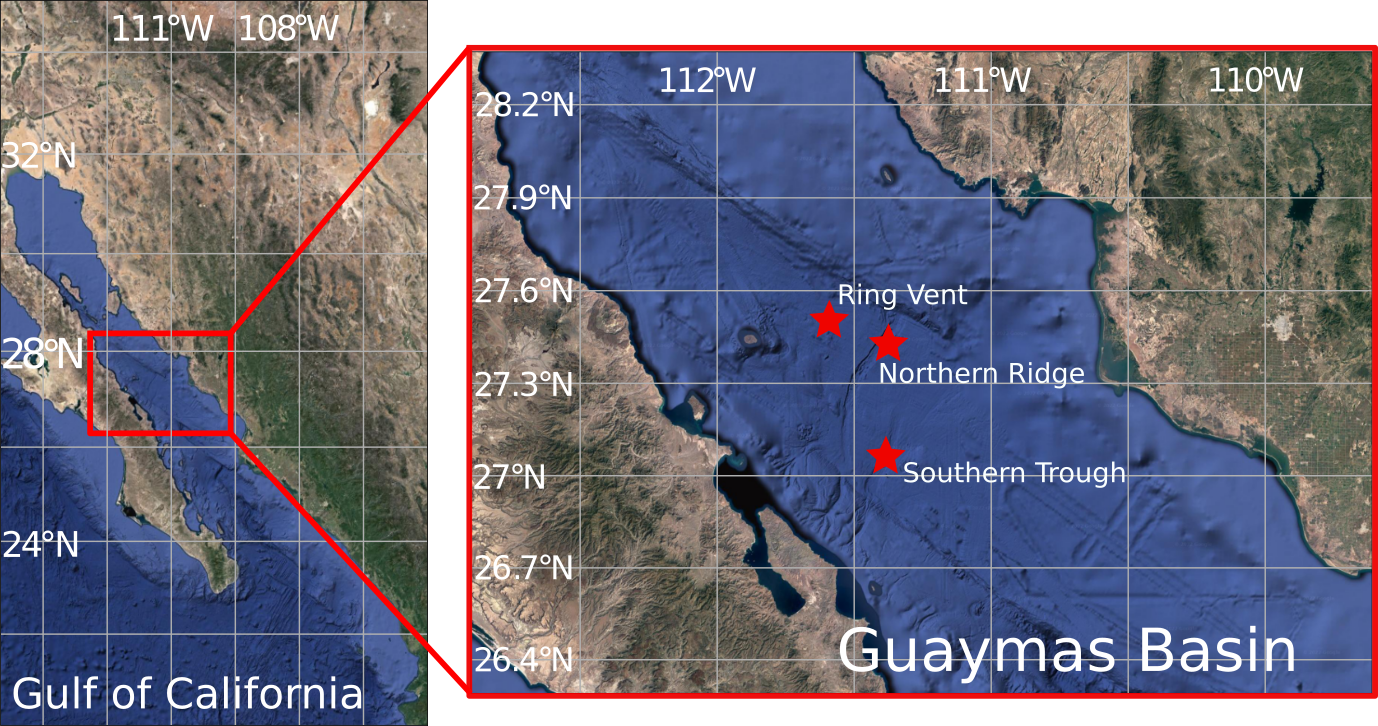
\includegraphics[width=\columnwidth]{figures/ops_guaymas.png}
  \caption[Guaymas Basin, Gulf of California.]{\textbf{Guaymas Basin, Gulf of California.} The Gulf of California and the Guaymas Basin within it are visualized with satellite imagery and composite satellite and open-source bathymetry (as provided by GoogleTiles). The Southern Trough, Northern Ridge, and Ring Vent are marked with stars; the Northern Ridge and Ring Vent were of particular focus during research cruise RR2107.}
  \label{fig:ops_map}
\end{figure}

There are two axial troughs (spreading segments) in the Guaymas Basin, commonly referred to as the Northern and Southern Trough. There has been a long documented history of hydrothermal expressions in the Guaymas Basin, with a particular focus on the Southern Trough\footnote{e.g., \autocite{ondreas2018recent, teske2016guaymas, seewald1994variations, von1985chemistry, lonsdale1985hydrothermal}}. RR2107 was uniquely focused on studying two Northern sites at or near the Northern Trough: Northern Ridge and Ring Vent. Ring Vent is a diffusive off-axis venting site approximately \SI{28}{\kilo\meter} northwest of the Basin spreading center\autocite{teske2019characteristics}. Due to it's nature, ROV \emph{JASON} was primarily used at this site for geochemical surveys. AUV \Sentry studies were instead primarily focused on the Northern Ridge, a recently discovered hydrothermal site\autocite{soule2018exploration, geilert2018formation}, approximately \SI{1850}{\meter} underwater and at the edge of an additionally \SI{300}{\meter} deeper graben. The ridge is approximately \SI{600}{\meter} long and features several tall sulfide structures 10-\SI{25}{\meter} in height with active smoking along their bodies. A smoking ``chimney'' at the northernmost point of the ridge was targeted for autonomous plume-charting, although the entire ridge was studied during RR2107 activities. The chimney vent is composed of a cluster of tens of small orifices ($<$\SI{0.1}{\meter} diameter) that can create up to an approximately \SI{1.5}{\meter} diameter chimney base. The fluid produced is thick with particulate matter and highly-enriched in carbon dioxide, hydrogen, and methane. Measured with a temperature wand on ROV \emph{JASON}, fluid temperature at the vent orifice is estimated to be \SI{340}{\celsius} and the fluid visually ventilates rapidly\footnote{In contrast, the ambient seawater is methane-poor, considerably less turbid, and cold at \SI{4}{\celsius}}. As vent fluids rise and form a plume at this site, the ambient water mixes (entrains) at an unknown rate, and advects by mild deep-water currents estimated to be approximately \SI{0.15}{\meter\per\second} at it's peak during the expedition. Under these conditions, plume expressions could be transported several kilometers from a known source, and would be expected to rise over \SI{200}{\meter} in the water column\autocite{speer1989model}.

The RR2107 expedition had several key objectives: test novel \emph{in situ} instruments to measure dissolved methane\autocite{kapit2021dissolved,kapit2021measurement,michel2022gas}, test novel \emph{in situ} instruments to measure the carbonate cycle, map the heat distribution in shallow sediments above hydrothermal sills\footnote{In extension of, e.g., \autocite{neumann2022heat}}, collect tubeworm and geological specimens, and collect biological samples of microbiota in hydrothermal plume-fluids to re-construct the structure of a plume microbiome. It is typical that research cruises have several science teams working together under an appointed chief scientist to maximize the use of ship assets while at sea, and this cruise was no exception. To enable science operations, AUV \Sentry, ROV \emph{JASON}, and standard oceanographic equipment (i.e., Conductivity-Temperature-Depth (CTD) rosette, Niskin carousel, shipboard acoustics) were available. The deployment of autonomy on the cruise for \Sentry operations was coupled with objectives to test \emph{in situ} instruments and collect microbiota samples. For both of these tasks, charting different regions within a plume is important to test the capabilities of the novel instruments and to collect biological samples from a diversity of plume-conditions.


\section{Challenges for Robots and Autonomy in the Deep Ocean}
\label{sec:ops_challenges}
% No GPS, no satellite, only acoustics, very few observatories, etc.
In the Guaymas Basin setting, or any deep ocean research, there are several unique challenges to deploying robotic platforms in contrast to terrestrial applications. Perhaps the most quintessential of these challenges is the conductive nature of water, and its corresponding attenuation of radio frequencies\autocite{qureshi2016rf}. The natural consequence is that ubiquitous terrestrial technologies leveraged by robots and humans alike, such as global positioning satellites (GPS), imaging satellites, and radio-based wireless communication, are not available for underwater navigation, mapping, or communication. The most common alternative for wireless communication underwater are acoustic waves, which can travel hundreds of kilometers and can be used effectively for ranging (e.g., estimating distance and angle between a source and reflector), but have a significantly reduced data transmission rate\autocite{qureshi2016rf}. Global positioning of an underwater platform is typically done via acoustic ranging with a ship, the ship then having access to GPS to perform an appropriate coordinate transformation for the robot. While accurate, the bit-rate and time-of-flight for information transmission is generally not sufficient for constant localization of a vehicle (let alone also requiring a ship to maintain proximity to a platform, and forgo communicating other types of information), and so many state-of-the-art underwater vehicles use a form of ``dead-reckoning'' to estimate their position with inertial sensors. The use of Doppler velocity loggers (DVL), downward facing acoustic sensors that estimate velocity relative to another object, has improved the overall accuracy of dead-reckoning for near seafloor (within \SI{150}{\meter}) navigation\autocite{stutters2008navigation,liu2022dvl,fong2006evaluation,rigby2006towards}. To us a DVL requires proximity to the seafloor (within tends of meters) in order to provide a ``bottom-lock'' useful for navigation; this further restricts an AUV's navigational freedom.

Beyond navigation and communication, the challenge of working in water necessarily impacts that type of scientific sensing that can also be accomplished. Light, just like radio, is also severely attenuated in water; sunlight typically only penetrates the ocean to about \SI{200}{\meter}, and up to \SI{1000}{\meter} in the best conditions\footnote{Depths between 200-\SI{1000}{\meter} are aptly part of the ocean's ``Twilight Zone''\autocite{martin2020oceans}}. This means that vision based technologies, which have enjoyed significant development in robotics for e.g., autonomous driving tasks, are entirely restricted to either shallow depths or very near seafloor studies, in which light sources carried by a platform might be used\footnote{Of course, navigating in the water column near no other structure is not necessarily a setting for which vision-based navigation may be useful, even if there was light.}. Other common optical-based sensors in robotics, such as Lidar, are similarly difficult to use underwater due to attenuation and refraction. This is not to say that there are no optical sensors that can be used underwater. For short distances, transmitted light between a source and receiver can be used to estimate water turbidity\autocite{bishop1999transmissometer}. Light can also be used to transmit information between a source and a receiver at a higher bitrate than acoustics over modest distances (tens of meters)\autocite{qureshi2016rf,farr2010integrated}. Other sensors may use light, but in creative ways---for instance, oxygen optodes detect luminesence of a chemical reaction that corresponds to a measure of dissolved oxygen\autocite{nicholson2017air}, and laser-based spectrometers have been put in depth-capable housing and use membrane inlets to accept gaseous samples to analyze\autocite{wankel2010new}. While many of these technologies are still in their nascent development phase, perhaps one of the most ubiquitous sensors in oceanography (other than acoustic instruments) is the conductivity-temperature-depth (CTD) probe, which uses induction to measure salinity, resistivity to measure temperature, and a pressure sensor to measure depth\autocite{rudnick2007underway}. With these measurements, computation of density is possible, which is the primary driver of water mass mixing in the ocean. 

No matter the sensor, water-column sensing and mapping in the deep sea relies on collecting point observations and reconstructing fields of interest from these incredibly sparse data.
To address this data sparsity issue, there are several large-scale efforts that contribute to the instrumenting and global understanding of the ocean. Argo, an international network of thousands of small buoyancy-controlled floats which drift in the ocean and take basic \emph{in situ} measurements (e.g., temperature, salinity) of the water column up to \SI{6000}{\meter} in depth is one such example\autocite{roemmich2009argo,jayne2017argo}. With a finer degree of control, small glider networks operated by the e.g., Ocean Observatories Initiative (OOI)\footnote{\url{https://oceanobservatories.org/marine-technologies/gliders/}, \autocite{trowbridge2019ocean}}, offer an opportunity for remote targeting of particular regions or depths to study larger-scale phenomenon. Several highly instrumented ``observatories'', such as Martha's Vineyard Coastal Observatory\autocite{austin2000martha} or the Endurance Array in the Northeast Pacific\autocite{barth2018warm}, also serve an important role for collecting highly temporally resolved data at specific sites. It is certainly the case that there is a lot of ocean data; what has yet to be standardized is how to leverage this data for enabling targeted research studies, particularly with highly capable robotic platforms. Central to this challenge is that despite a wealth of data, the ocean is truly vast; in 10 years of available records from Argo, there are no records of a float in the Guaymas Basin\footnote{As determined via the Euro-Argo data exploration tool, accessed November 20, 2022.}. There are no instrumented arrays in the Gulf of California. And glider or robotics studies conducted there have been part of singular research cruises conducted by disparate research teams, with mixed data discoverability and accessibility. 

While initiatives like the UN Ocean Decade\footnote{\url{https://www.oceandecade.org/}} and the NASA EarthData open science program\footnote{\url{https://www.earthdata.nasa.gov/esds/open-science}} stand to transform the challenge of finding data, practically, oceanographic researchers are prepared to continue to be self-sufficient for any given expedition.
For a roboticist, this requires becoming familiar with prior research at a given site (if available) to contextualize how certain sensors will map to a task at hand, the scientific instruments on a vehicle and their operating principles, and the activities of other science team members to effectively share data within the party. Understanding on all of these axes helps to identify any instrumentation gaps for robotic tasks prior to boarding a vessel (so they can be either rectified by preparing new instrumentation, or the impact mitigated by identifying useful proxies), effectively leverage the expertise of the entire science team to inform missions while underway, and clarifies the design of the post-cruise data products to support science objectives.

\section{The Science Party and Responsibilities}
%Establish how computer scientists fit on a ship.
Before a robot even touches the water, a massive amount of operational overhead is necessary to support deep sea studies. In general, deep ocean research requires using an oceanographic vessel. The R/V \emph{Revelle} is one of several ships in the University-National Oceanographic Laboratory System (UNOLS) network of research ships available through federal support by the United States\footnote{Private research institutions outside of this network, like the Schmidt Ocean Institute, also provide some global-class ships available for deep sea research.}. The R/V \emph{Revelle}, operated by the Scripps Institution of Oceanography at the University of California, San Diego\footnote{\url{https://scripps.ucsd.edu/ships/revelle}}, is a 273 ft vessel constructed in 1996 and completed a mid-life retrofit in 2020. The \emph{Revelle} houses 21 crew and 37 science staff for any expedition. A 4000 sq ft laboratory space dominates one deck of the ship, containing storerooms, a computer lab, a science freezer, and wet lab (among other spaces). The ship is additionally equipped with acoustic surveying equipment, a rosette bay and winch, chemical hoods and storage, dredges, and weather stations in addition to general office equipment. Any additional equipment---AUVs, ROVs, specialized sensing equipment, laboratory equipment, computers---is carried on by the science party.

Captain and crew on a research vessel are responsible for the overall safety of the operations, and are key stakeholders in all operations. Marine technicians are crew members that specialize in the scientific instrumentation and infrastructure on a ship, directly working with the science team to assist with deployments and data curation. The science party itself can be a professionally diverse group of trainees, scientists, and engineers from multiple fields. On RR2107, the science party comprised \Sentry and \emph{JASON} teams (approximately 14 personnel), two teams from Woods Hole Oceanographic Institution (WHOI) comprising engineers, computer scientists, and geochemists (approximately 10 personnel), a team from Harvard University and affiliates in biology, geochemistry, and microgenomics (approximately 4 personnel), and a team from Centro de Investigaci\'on Cient\'ifica y de Educaci\'on Superior de Ensenada (CICESE) comprising geodynamicists (approximately 2 personnel); all teams included graduate students. Everyone on a research vessel not only works together, but must live together for the duration of the expedition. This makes oceanographic research (and any ``expeditionary'' travel) a highly unique working environment\footnote{As late as the 1960s women were barred from working on oceanographic vessels, and this unique working environment can lead to modern inclusivity challenges. Recognition of long-standing challenges to diversity and inclusion in oceanography has inspired new curricula for aspiring chief scientists to design supportive at-sea environments, e.g., \url{https://cobra.pubpub.org/}} in which every member is necessary for making the experience productive and supportive.  

For a field roboticist, being a supportive team member may mean performing more than just \Sentry or \emph{JASON} operations. Literacy in certain data processing and visualization tools, comfort with network protocols and a command line, and hands-on experience working with certain sensors can prove to be extremely useful to other science activities while aboard. Coordinating with other science teams prior to an expedition can be a way to identify areas in which a computer scientist or a roboticist could be helpful. For instance, prior to RR2107, a desire to monitor \Sentry science data while it was underway was expressed. While outside of the direct purview of the autonomy operations, creating a tool that listened to a local network on the ship and displaying data that came over the network in a live visualizer was a relatively straightforward process and provided the science team with a ``real-time'' view of \Sentry operations, informative for other activities. In practice, a field roboticist has a lot of tools that they bring with them on an expedition; there is increasing interest in using more of those tools for oceanographic missions as data infrastructure and use of \emph{in situ} sensors accelerates.  

\section{AUV \Sentry}
AUV \Sentry, operated by the National Deep Submergence Facility (NDSF) at WHOI\autocite{kaiser2016design} is a general purpose platform with depth capability up to \SI{6000}{\meter} (\cref{fig:ops_sentry}). \Sentry is the successor of \emph{ABE}\autocite{yoerger1991autonomous}, the first widely utilized AUV for deep ocean research by the U.S. oceanographic community. \Sentry has completed upwards of 600 dives, and is equipped with three classes of instruments: vehicle sensors, geophysical sensors, and oceanographic sensors. Vehicle sensors are largely those that assist with AUV localization; geophysical sensors include acoustic multibeam, subbottom profiler, and magnetometers, which are useful for collecting bathymetric and sub-seafloor maps. For plume studies, the oceanographic sensors are of primary interest, and include a CTD, optical backscatter (OBS) instrument, oxygen optode, and oxidation reduction-potential (ORP) sensor. Each oceanographic sensor is synced to a shared precision clock on \Sentry, and logged to separate files at the manufacturer recommended sampling frequencies. In addition to the standard sensor suites, \Sentry can accept some novel instrumentation developed by a science party for an expedition. During RR2107, two novel methane sensors were integrated into \Sentry to complement the oceanographic sensors for hydrothermal plume charting\autocite{michel2022gas,kapit2021dissolved,kapit2021measurement}.

\begin{figure}[h!]
  \centering
  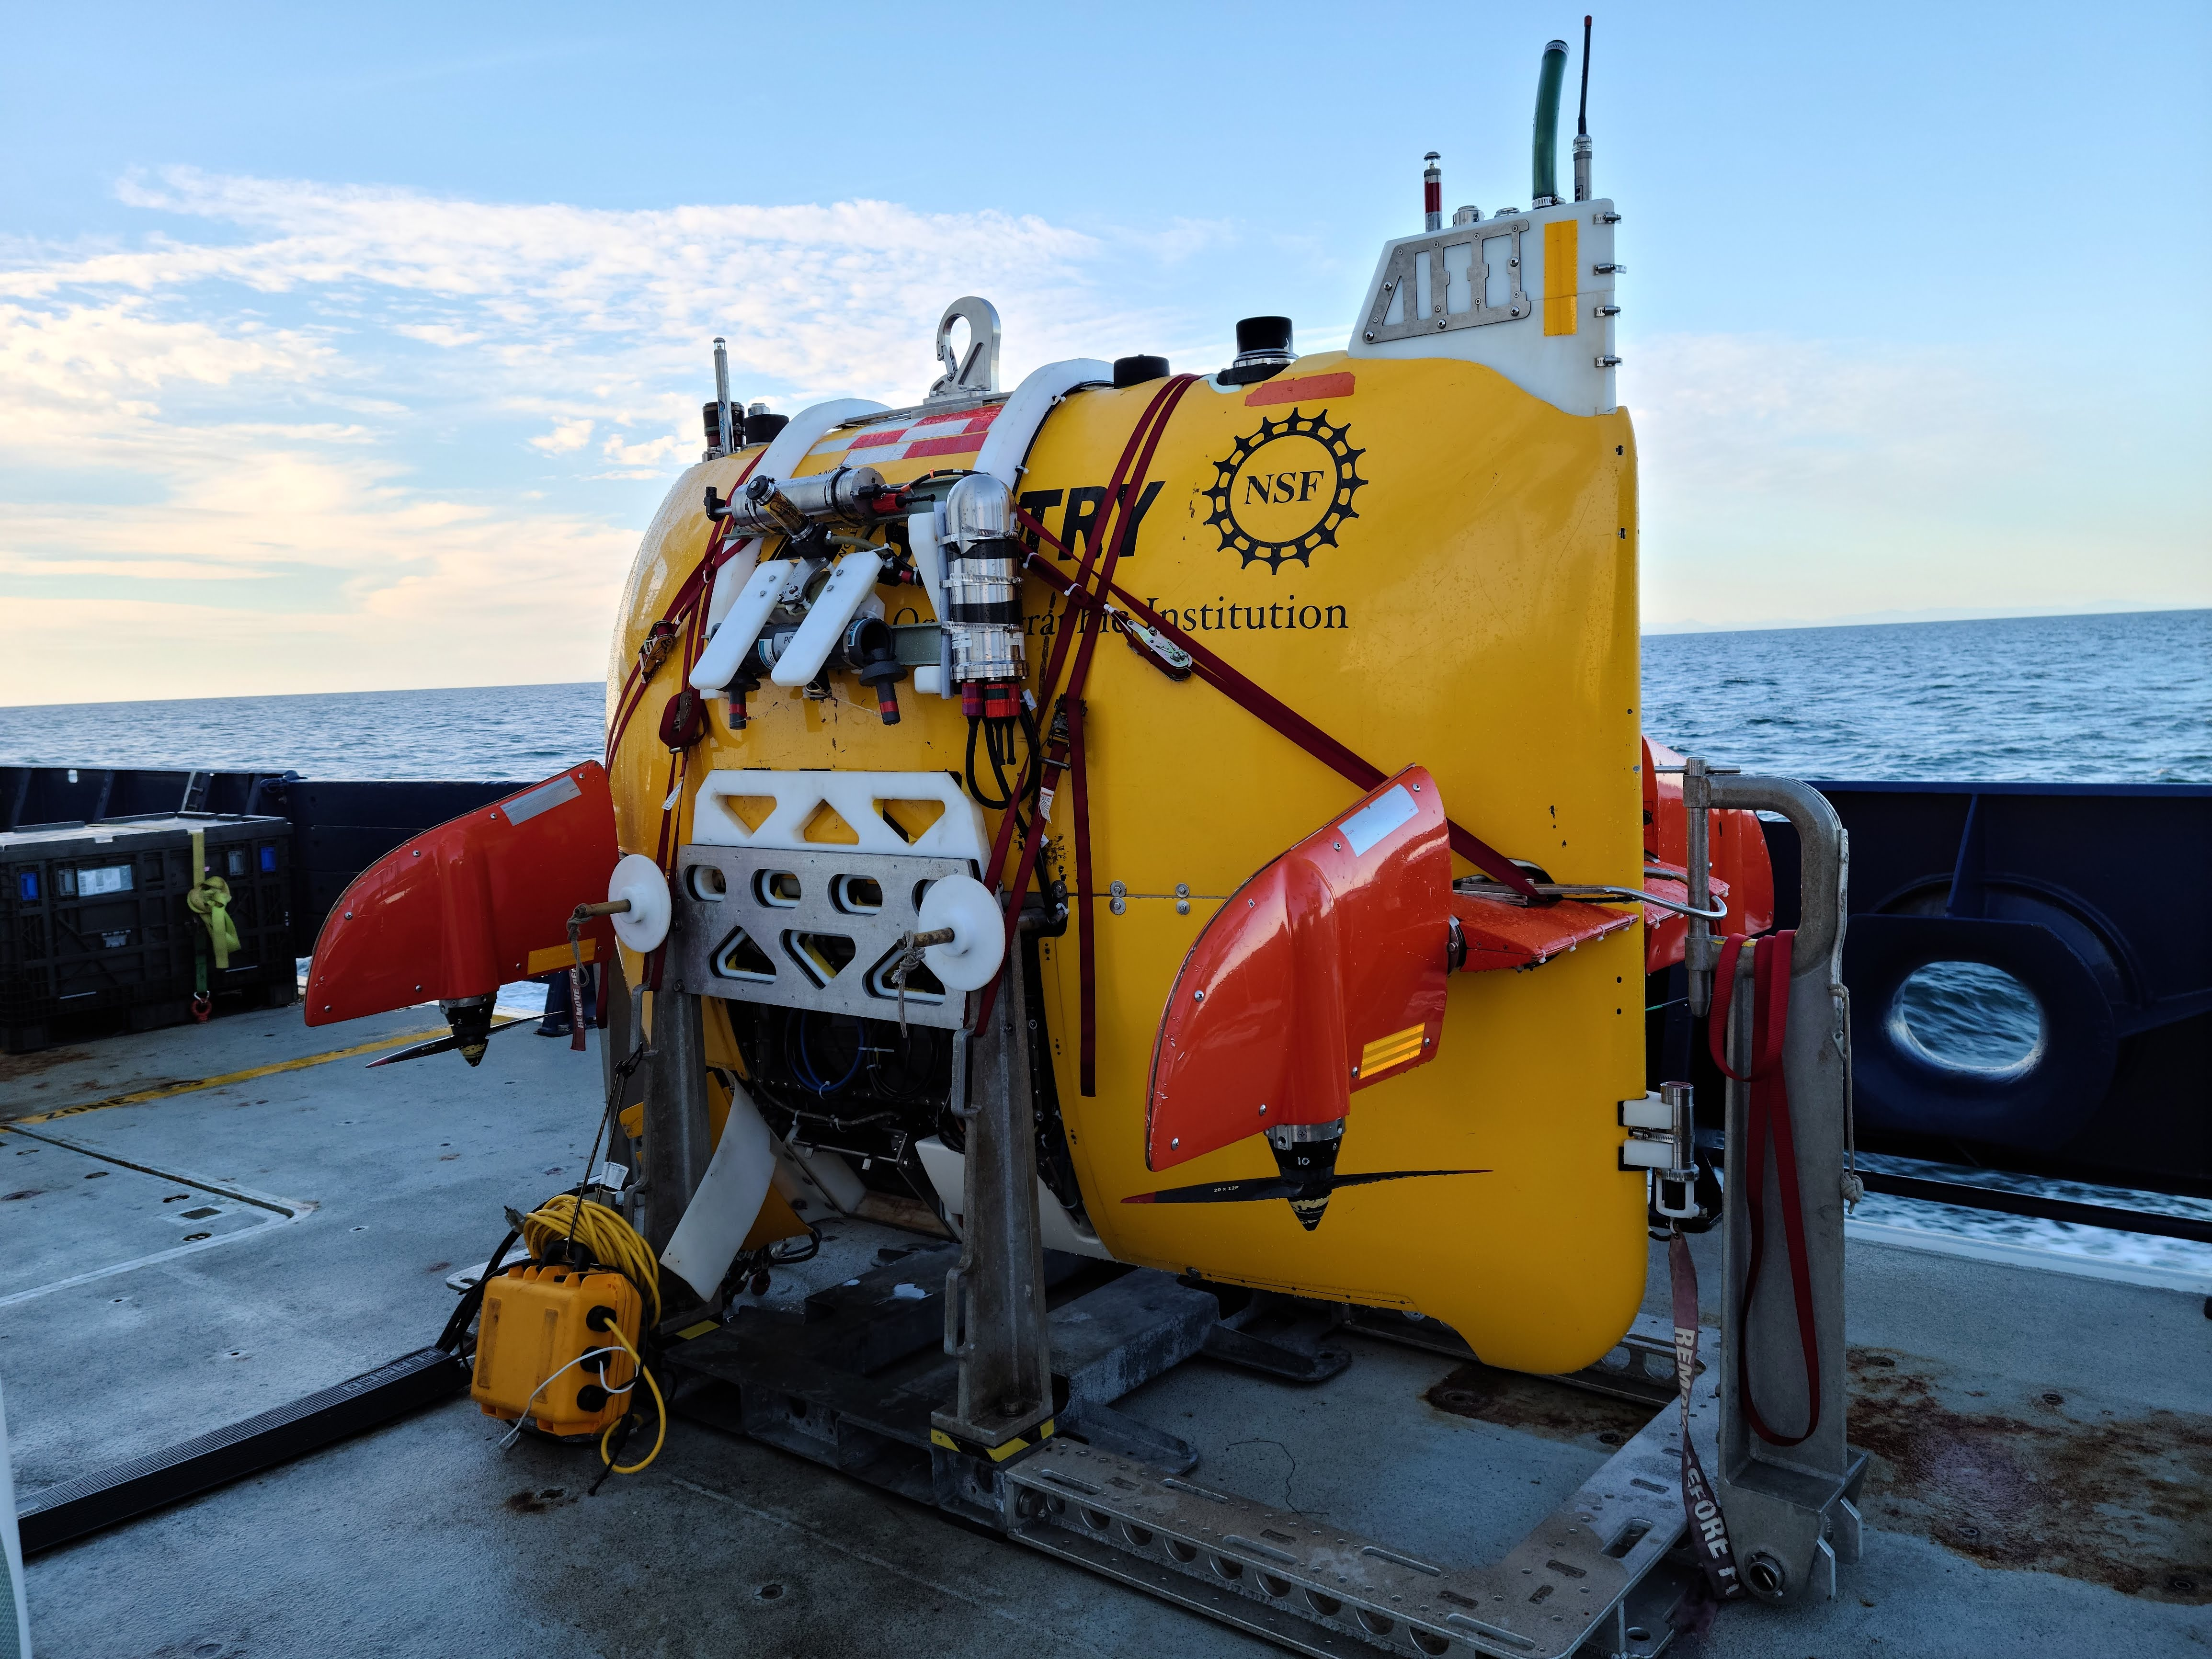
\includegraphics[width=0.8\columnwidth]{figures/ops_sentry.jpg}
  \caption[AUV \Sentry]{\textbf{AUV \Sentry}. A picture of AUV \Sentry on deck of the R/V \emph{Revelle} during RR2107 activities.}
  \label{fig:ops_sentry}
\end{figure}

The \Sentry team for an expedition has an appointed expedition leader, who interfaces directly with the Chief Scientist and any other relevant science parties to plan \Sentry dives. The team is largely responsible for the physical and virtual safety and maintenance of \Sentry during an expedition. As such, the expedition leader is additionally responsible for confirming the safety of every dive plan and managing pre-dive and post-dive checks. Safety confirmation of a dive plan formally requires passing a simulation dive of the plan using a set of scripts maintained by the \Sentry team. This simulation uses bathymetry and marginal environmental estimates to assist in checking a plan for obstacle clearance, in addition to computing possible localization drift (associated with number of turns) among other heuristics. Less formally, the expedition leader has final call on whether a dive is feasible, and may use contextual knowledge of a location or the vehicle state to deny or suggest changes to a plan. For instance, Guaymas Basin has a notably soft seafloor due to sediment deposition. This impacts the quality of DVL estimates, which in turn impacts the quality of \Sentry localization. This lead to adjusting the altitude restriction for \Sentry during RR2107 to reduce risk to the vehicle.


\section{ROV \emph{JASON}}
ROV \emph{JASON}, like AUV \Sentry, is also operated by the NDSF at WHOI\autocite{ballard1993medea,yoerger1986jason,petitt2004power} and has been in operation since the late 1980s (\cref{fig:ops_jason}). Distinct from \Sentry, \emph{JASON} is connected to a ship via a cable which transmits information and power. This allows real-time sensor and visual feedback from the ROV and fine remote control of the vehicle navigation and two manipulator arms. \emph{JASON} is a particularly powerful tool, as it can literally ``put eyes'' on the seafloor, and perform physical sample collection tasks that AUVs cannot, including sediment coring, microbial mat retrieval, macro-flora/fauna and rock sample collection, and water sampling. Standard oceanographic equipment, like CTD, optode, and turbidity sensor are mounted to \emph{JASON} and logged in a similar fashion to \Sentry equipment. \emph{JASON} can additionally accommodate carrying novel equipment brought by a science party, however this equipment must be certified before integration on \emph{JASON} for the desired depth they are to be deployed. 

\begin{figure}[h!]
  \centering
  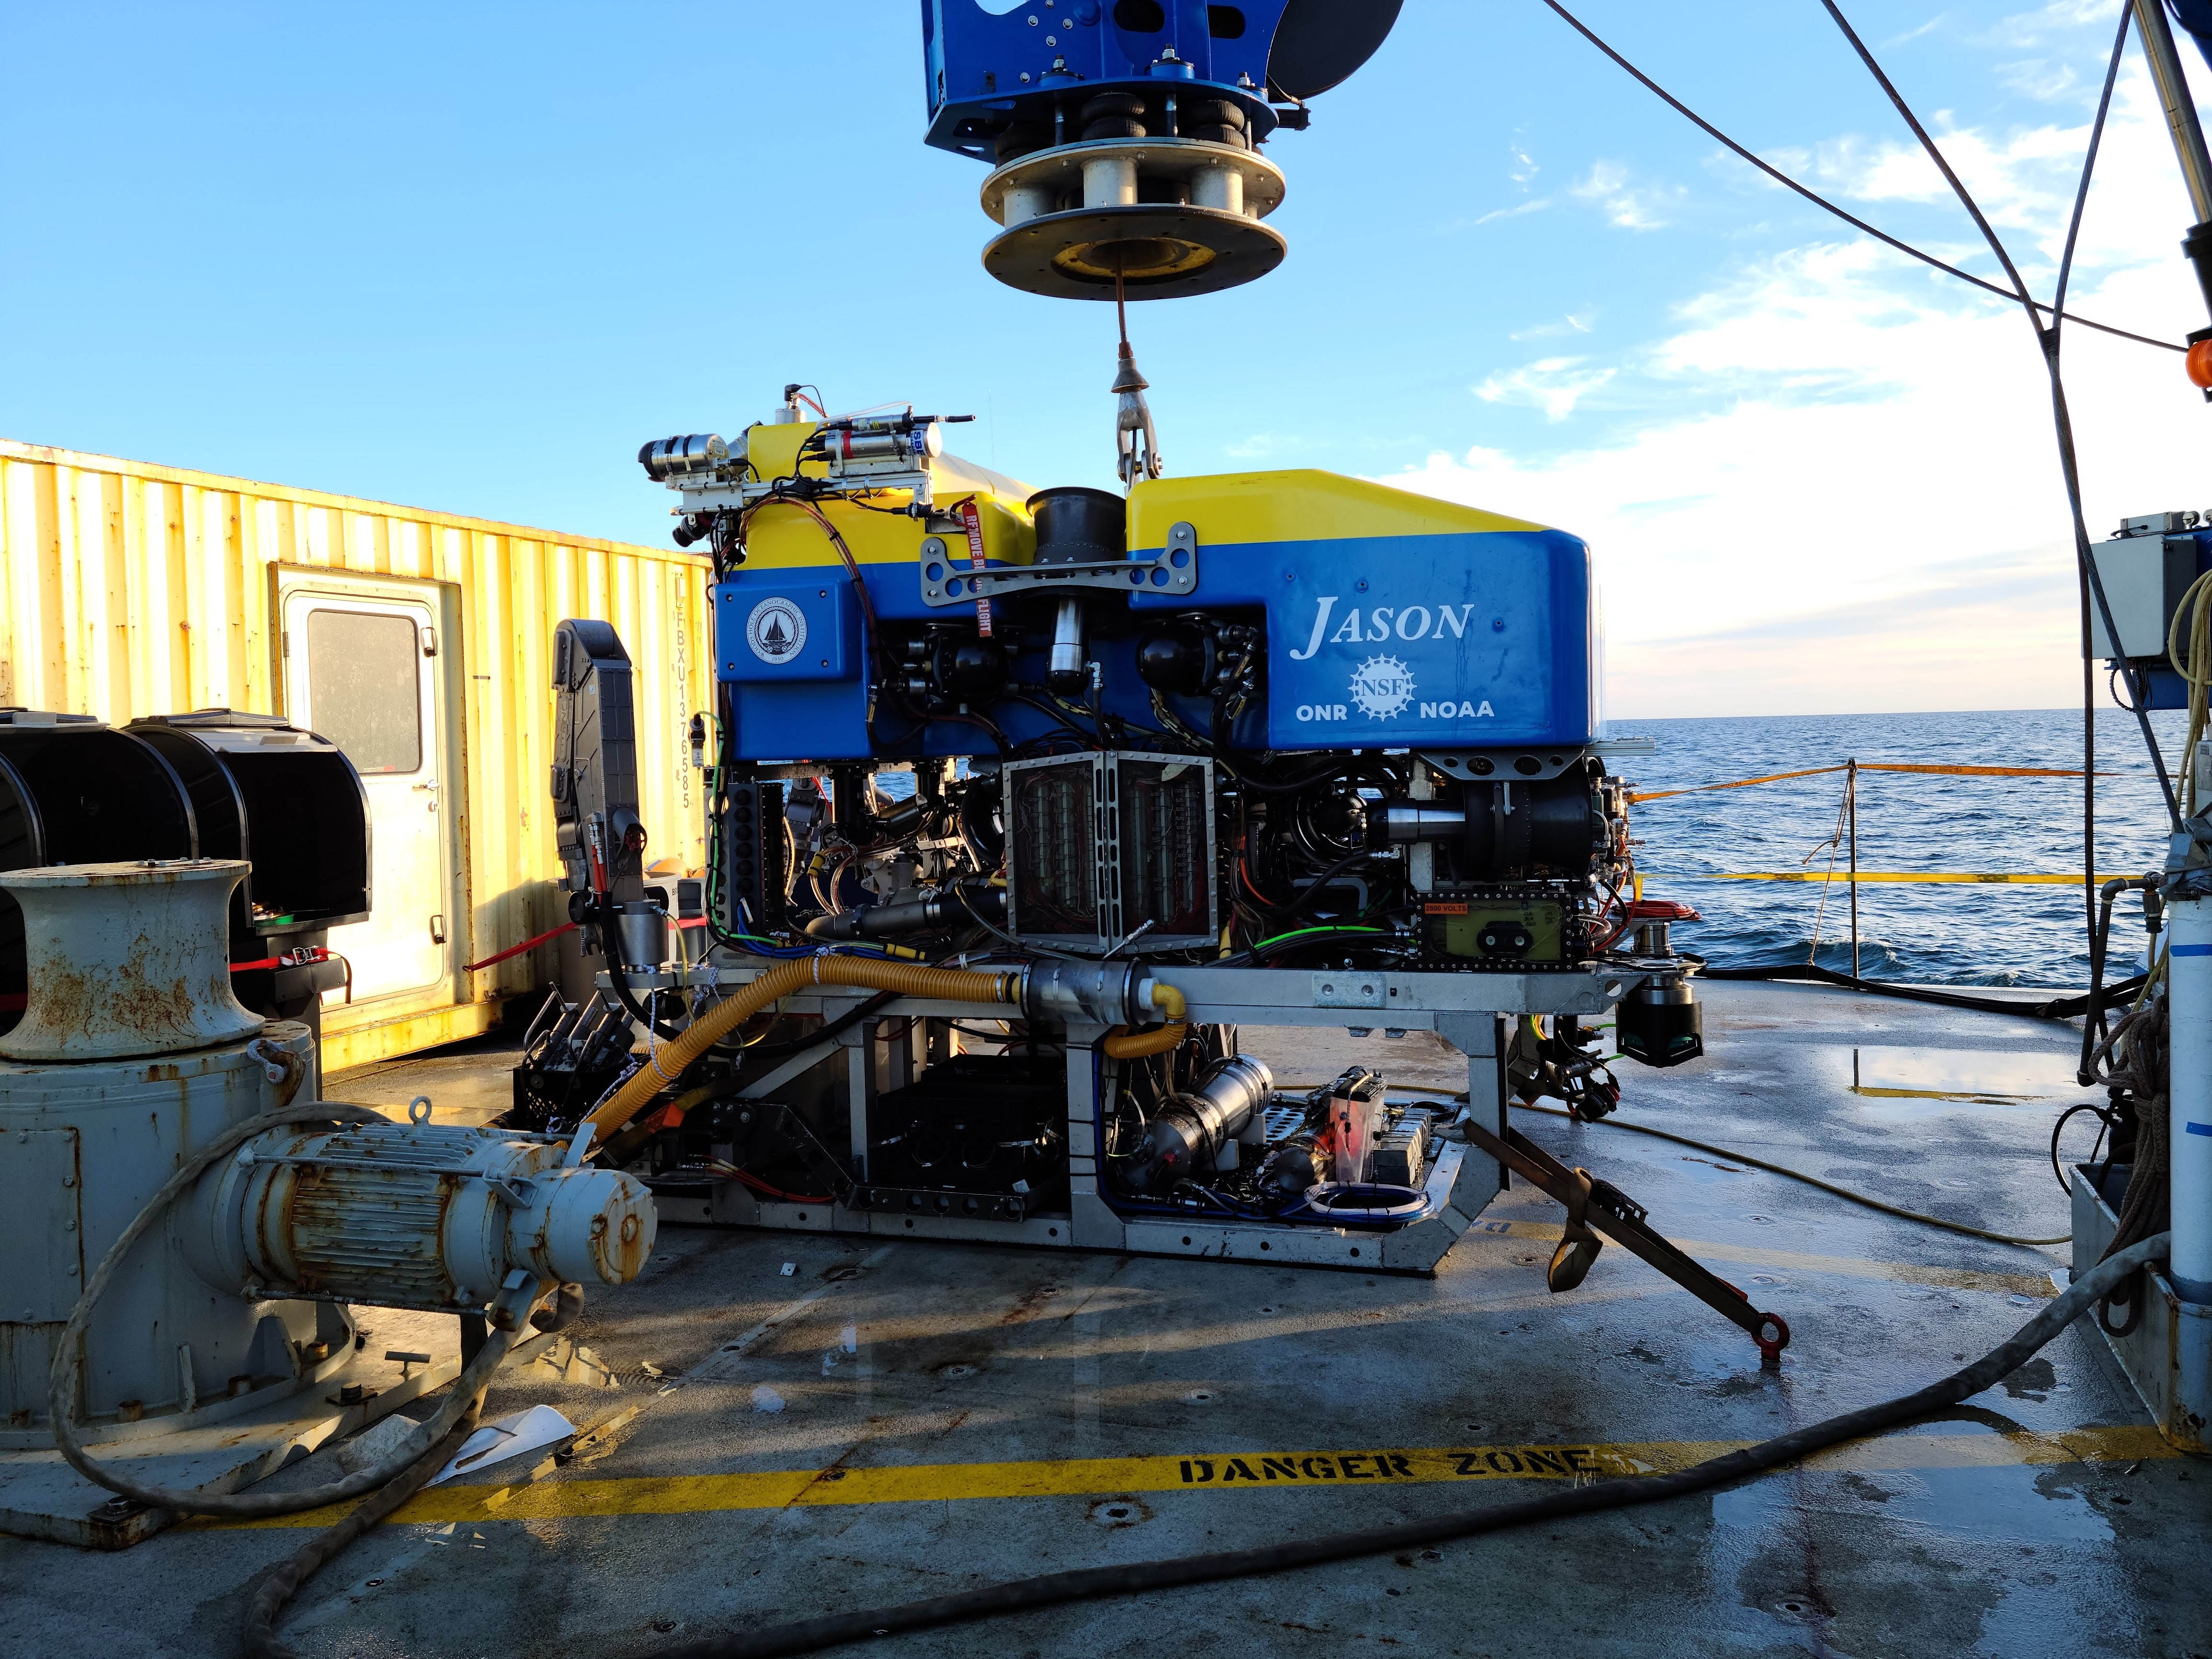
\includegraphics[width=0.8\columnwidth]{figures/ops_jason.jpg}
  \caption[ROV \emph{JASON}]{\textbf{ROV \emph{JASON}}. A picture of ROV \emph{JASON} on deck of the R/V \emph{Revelle} during RR2107 activities.}
  \label{fig:ops_jason}
\end{figure}

While being operated, three \emph{JASON} engineers act as ``pilots'' in rotating shifts throughout a dive (which can be over 24 hrs long). These piloting operations occur in the ``control van'', in which data servers/ship-side data loggers, computer monitors, and annotation stations are set-up. At least three science party members are also required in the control van during operations---a dive science leader and two annotators. The science leader interacts with the pilots and sets the activities for a dive (e.g., collect this rock, collect some video, navigate to a new location). The annotators listen to the science leader and pilots to keep a running log of science activities and any relevant information about a dive as it occurs. The annotated logs are used post-expedition to search through \emph{JASON} data. The science party is responsible for setting a schedule for dive science leaders and annotators. On RR2107, most members of the science party were assigned at least one 4 hour shift in a 24 hour period in which they would be on call for being in the control van if operations were underway.

\paragraph{Autonomy Study Activities}
ROV \emph{JASON} was a rich source of external data to assist with the autonomy study presented in this thesis. In particular, \emph{JASON} could physically observe the target vent and deploy additional sensing equipment to compensate for holes in \Sentry sensing capabilities for the expedition. As described briefly in \cref{chap:field_results}, \emph{JASON} was used to:
\begin{itemize}
  \item Estimate the fluid temperature at a vent orifice with the temperature wand; measured \SI{340}{\celsius}.
  \item Estimate the size of a chimney and vent via still imagery.
  \item Deploy MISO cameras at a vent site, used to estimate the fluid exit velocity at a vent via video.
  \item Deploy current tiltmeters at various locations on the seabed to estimate deep currents at the autonomy test site.
\end{itemize}

While the first two activities are standard for \emph{JASON} studies, the latter two were specific to the operations in RR2107. 
MISO cameras, self-contained depth-capable GoPro devices\footnote{\url{https://www2.whoi.edu/site/miso/}}, were mounted to the brow and one of the arms on \emph{JASON}. Set to record in 4k, the arm-mounted camera was aligned to be approximately parallel with an active vent and used to record 1-5 min videos of turbulent plume fluids. The video was then processed following a \emph{JASON} recovery using particle imaging velocimetry (PIV)\autocite{zhang2019time}, which tracks turbulent ``parcels'' that have high cross-correlation between frames. By tracking many specific parcels over several frames, PIV methods can provide a vector field of velocity estimates, that can then be averaged to provide an estimate of mean flow in a region. Using MatLab's open source \verb|PIVLab|, a representative vent in the basin recorded during \emph{JASON} dive JD1390 at (27.4018606 N, 111.3991182 W, \SI{1809}{\meter} depth) was estimated to have fluid exiting at 0.7-\SI{1.33}{\meter\per\second} (\cref{fig:ops_miso}).

\begin{figure}[h!]
  \centering
  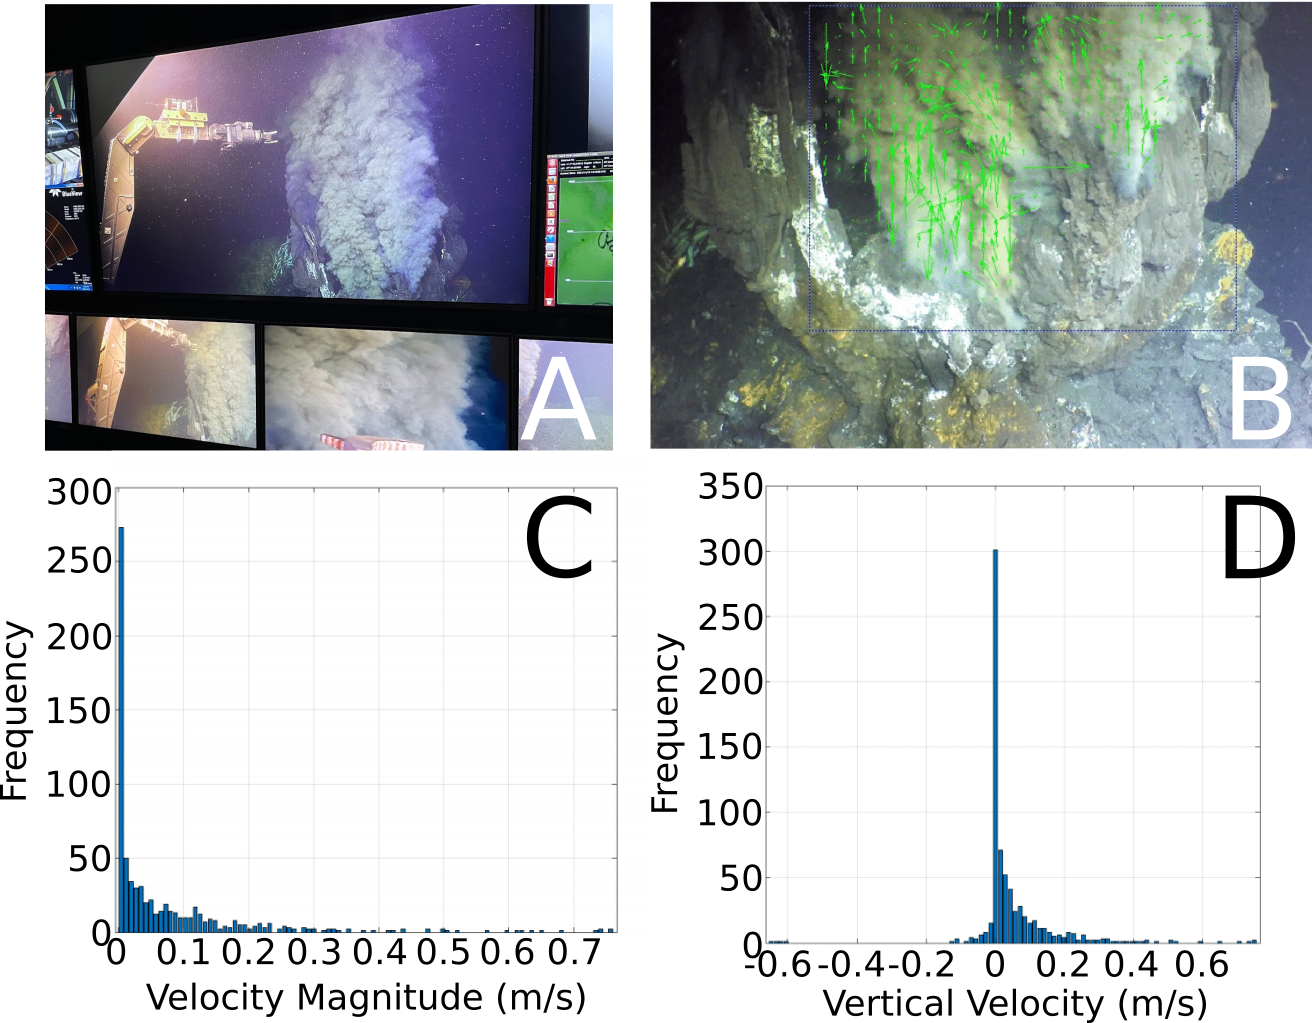
\includegraphics[width=0.8\columnwidth]{figures/ops_miso.png}
  \caption[Exit velocity estimation with WHOI-MISO cameras]{\textbf{Exit velocity estimation with WHOI-MISO cameras.}. A WHOI-MISO camera was mounted on an ROV \emph{JASON} arm and positioned to film exiting plume fluids from a hydrothermal vent (A). The capture video was processed using a PIV technique (B-D), which provides estimates of fluid velocity. The tails of the velocity field distributions may be indicative of exit velocities near orifices, as most of the imaged field is dominated by turbulent mixing within a meter of the orifices.}
  \label{fig:ops_miso}
\end{figure}

Tilt current meters\footnote{\url{https://lowellinstruments.com/}} are mounted to the seafloor by one point and are free to move under crossflow. The pose of the tiltmeter can be directly converted to crossflow magnitude and heading. ROV \emph{JASON} was used to alternately deploy 2 TCM-3 tiltmeters while performing other operations. \cref{tab:ops_tilt} shows information for each deployment. The first deployment of Tiltmeter A was the primary dataset used to generate an estimate of the current function used for the autonomy study. 

\begin{table}[h!]
  \centering
  \begin{tabular}{c|c|c|p{0.3\linewidth}}
      Tiltmeter & Dive Deployed/Recovered & Duration & Location \\
      \hline
      A & JD1389/-- & 28* hrs & (27.4006177 N, 111.3985321 W, \SI{1832}{\meter}) \\
      A & --/JD1390 & 28* hrs & (27.4002362 N, 111.3962494 W, \SI{1854}{\meter}) \\
      B & JD1389/JD1396 & 6 days, 15 hrs & (27.4006177 N, 111.3985321 W, \SI{1832}{\meter}) \\
      A & JD1392/JD1392 & 10 hrs & (27.4149571 N, 111.3873036 W, \SI{1840}{\meter}) \\
      A & JD1393/JD1393 & 20 hrs & (27.5001163 N, 111.6832265 W, \SI{1732}{\meter}) \\
  \end{tabular}
  \caption[Summary of tiltmeter deployments]{\textbf{Summary of tiltmeter deployments.} Two tiltmeters were deployed using ROV \emph{JASON} during RR2107 to estimate the magnitude and heading of deep currents. One tiltmeter was deployed for nearly 1 week, while another was deployed intermittently, so data products self-logged on the instrument could be used for autonomy ops. During the first deployment of tiltmeter A, the tiltmeter was moved to better align logistically with other \emph{JASON} operations.}
  \label{tab:ops_tilt}
\end{table}


\section{CTD Rosette}
A CTD rosette (or just rosette, \cref{fig:ops_rosette}), is a standard piece of oceanographic equipment which is typically an instrumented metal cage connected to a ship via a cable and used to collected vertical transects of the water column. Rosettes can also be towed laterally the water column if lowered and the ship driven in the pattern of the desired transect. Over the cable, data from the instrumentation on a rosette is streamed to a computer terminal on the ship. The depth is controlled by pulling in or releasing cable using a winch. The typical workflow is that one or more science team members are responsible for ``standing watch'' while a rosette is in operation, and communicates to a winch operator (always a crew member) via phone with requests to let out or pull in the cable.

\begin{figure}[h!]
  \centering
  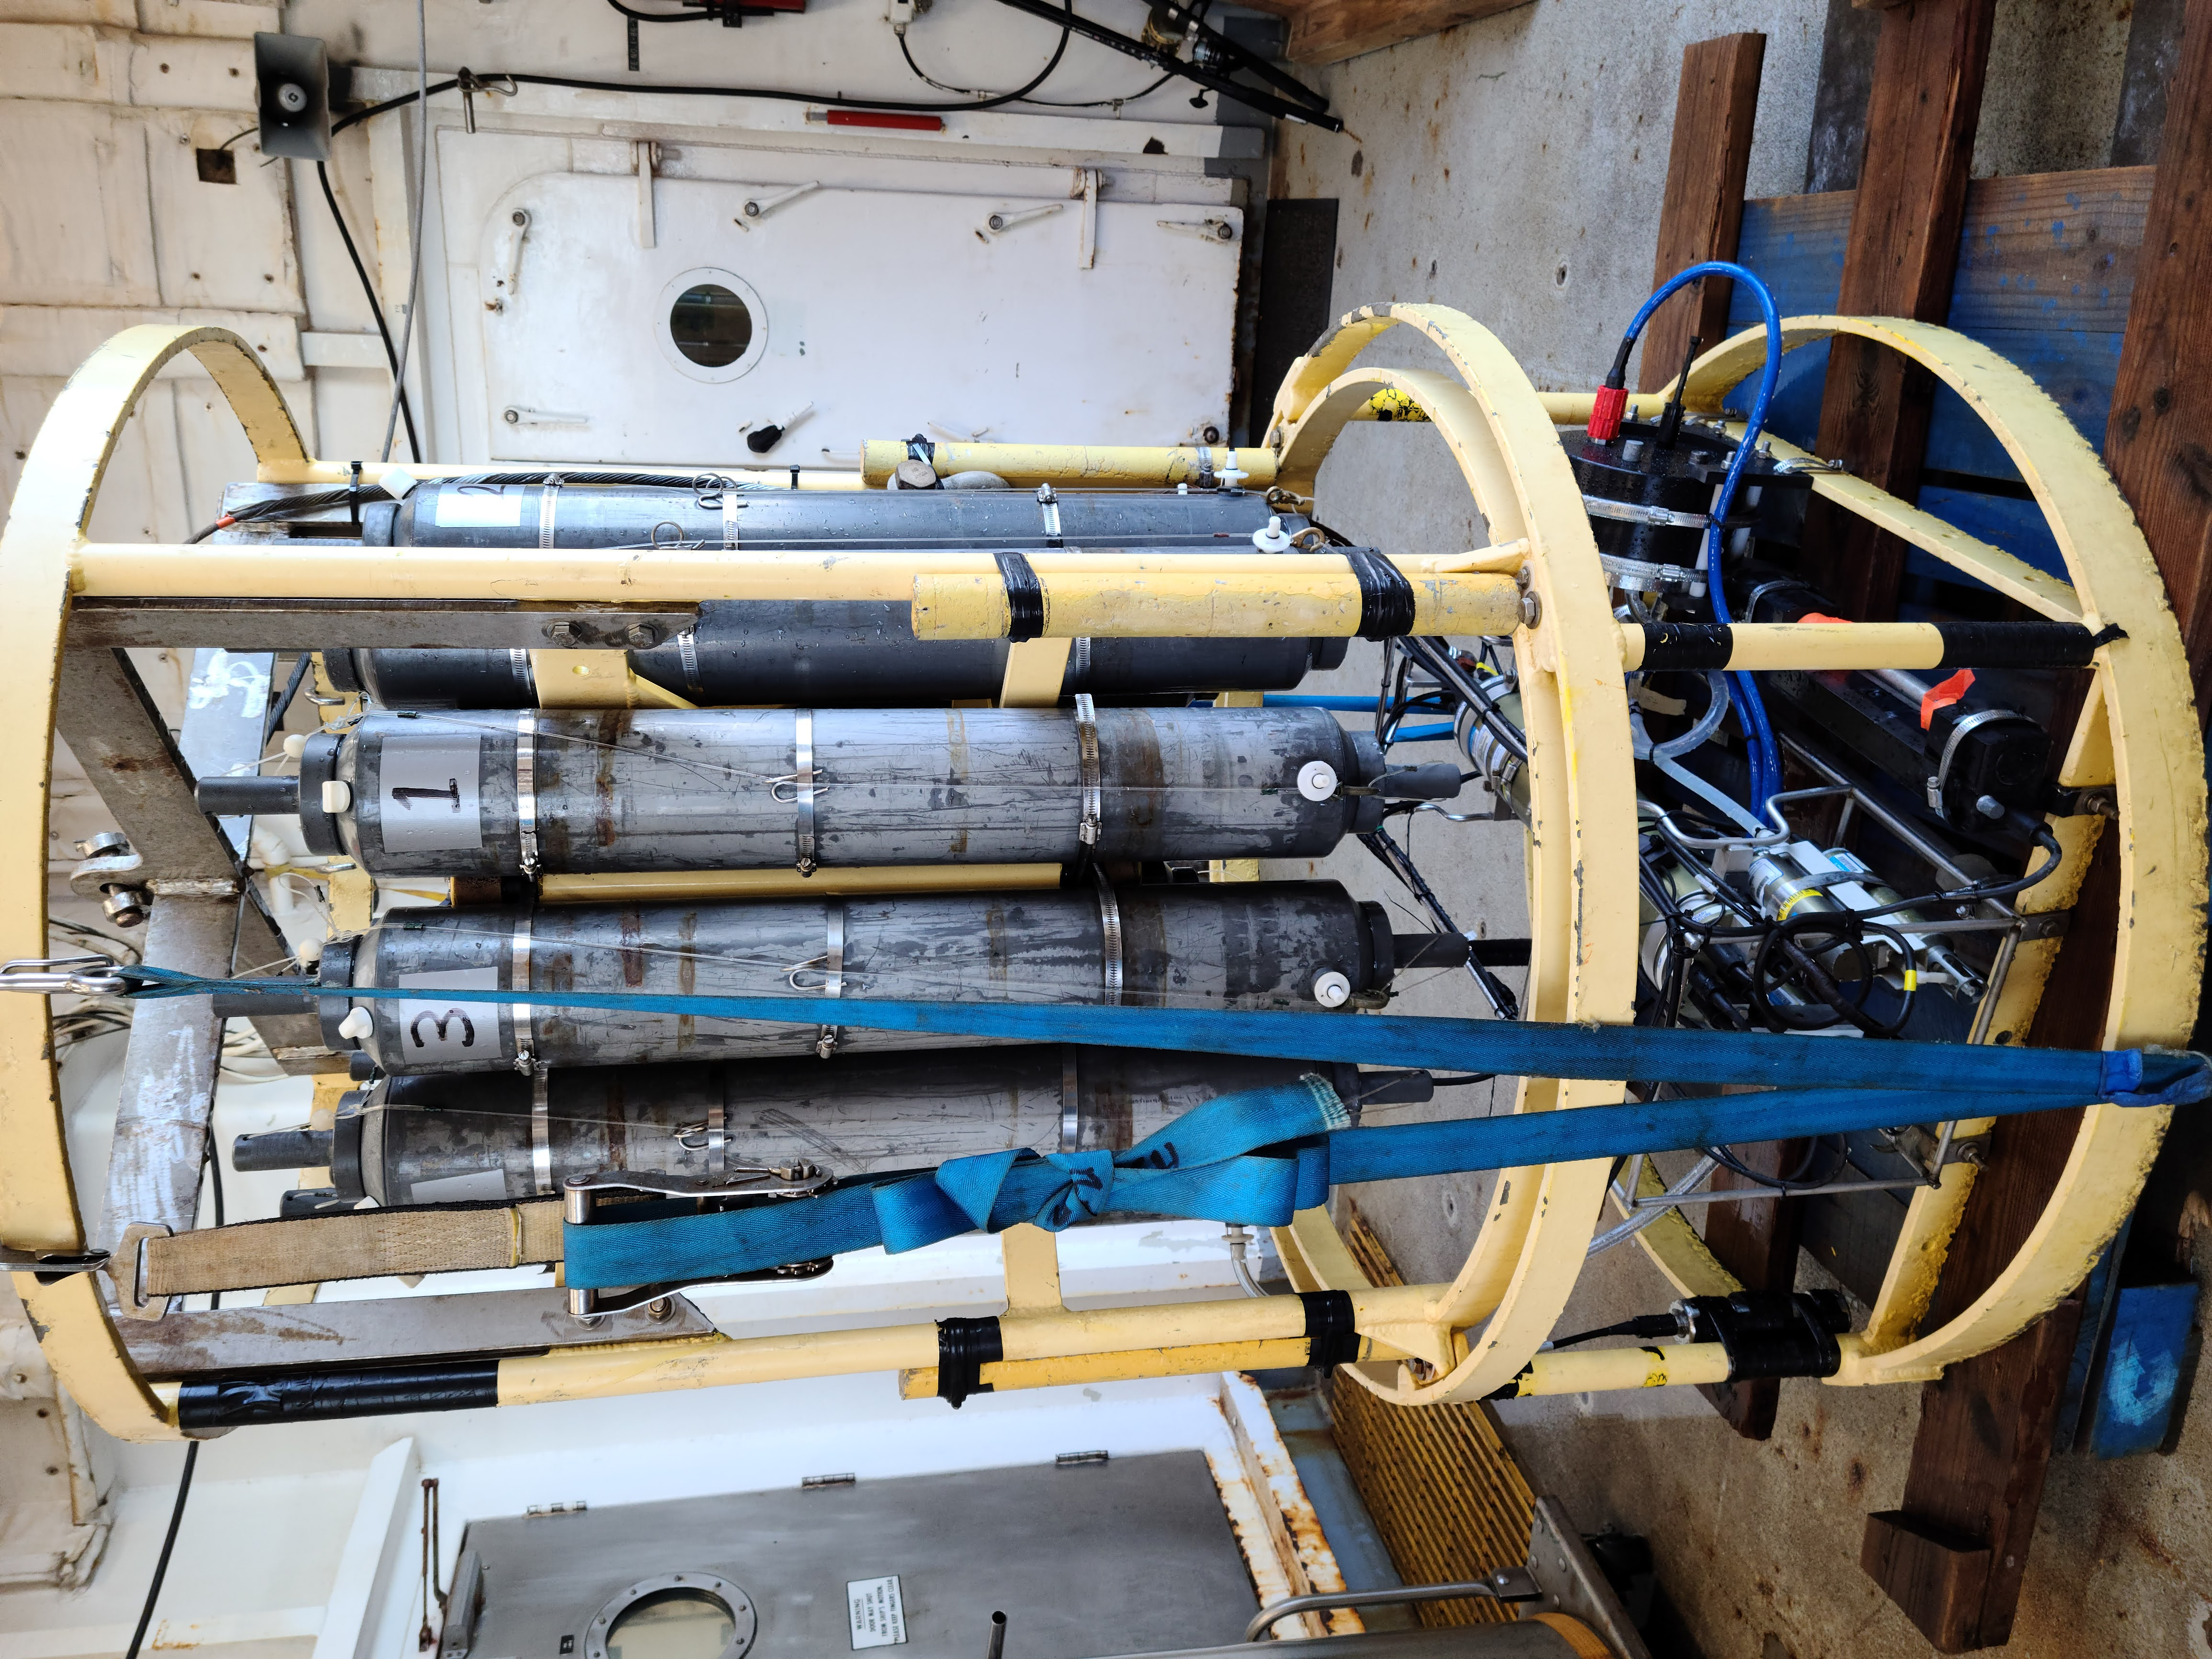
\includegraphics[width=0.8\columnwidth]{figures/ops_rosette.jpg}
  \caption[CTD Rosette]{\textbf{CTD Rosette}. A picture of the rosette in the rosette bay on R/V \emph{Revelle} during RR2107 activities.}
  \label{fig:ops_rosette}
\end{figure}


Equipment available on the rosette for RR2107 included CTD, flourometer, oxygen optode, and transmissometer (turbidity). All data is logged via a shared clock and in a proprietary format by Sea-Bird Scientific\footnote{\url{https://www.seabird.com}}, which was converted to CSV files while aboard the \emph{Revelle}. The rosette also had a 13-bottle Niskin bottle carousel. Niskin bottles are water containers which can be closed (``fired'') to seal water samples for \emph{ex situ} analysis. During rosette operations, Niskin bottles can be closed from the science team computer station by either pre-programming depths before a vertical transect, or by requesting a bottle fire via the monitoring application of the rosette while it is underway. Bottle samples during RR2107 were used to collect microbial samples, dissolved gas samples, and calibrate other \emph{in situ} instrumentation. 11 casts of the rosette were performed, 9 of which were standard vertical profiles. 

\paragraph{Autonomy Study Activities}
Within an analytical model for plume rise, density differences are computed in order to estimate buoyant force, which ultimately drives the estimated neutrally-buoyant layer height.
While standard stratification (density) profiles for the Atlantic and Pacific ocean basins are widely accepted\autocite{speer1989model}, the Guaymas Basin is a unique semi-closed system in the Gulf of California, and a stratification curve for background seawater in this Basin would lend itself to more accurate estimates of plume characteristics. As an AUV descends, it performs a vertical transect that could be used to compute this local stratification curve, however, since in RR2107 operations AUV \Sentry was typically targeted plume-impacted sites, and did not travel lower than an altitude of \SI{30}{\meter} for any operations, using profiles from the rosette would be advantageous. Using a set of subsampled points from every vertical transect collected by the rosette, a Gaussian Process (GP) was fit to the data, and the mean function used as the stratification curve used for autonomy tests.

  % description of the field setting
  \chapter{Discovering Hydrothermalism from Afar}
\label{chap:afar}

\begin{center}
    \begin{minipage}{0.7\textwidth}
      \begin{small}
      I had a blank canvas to fill with extraordinary possibilities, a fascinating jigsaw puzzle to piece together: mapping the world's vast hidden seafloor.\\ \emph{Marie Tharp}
      \end{small}
    \end{minipage}
    \vspace{0.5cm}
\end{center}

To track a spatiotemporal phenomenon requires first being able to sense it. There are two core challenges associated with perceiving hydrothermal plumes: existence (and availability) of technology and interpretation of heterogeneous data streams. With respect to deep-sea capable instrumentation, temperature, pressure, conductivity, and turbidity are all examples of quantities that can be near instantaneously measured by existing state-of-the-art \emph{in situ} sensors. However, for many geochemical quantities such as dissolved greenhouse gases (e.g., carbon dioxide, methane), few (if any) commercial sensors with rapid response times suitable for use on a mobile platform exist. This limitation has had severe impact on the ability for scientists to study phenomena like hydrothermal plumes, as these entities may be difficult to identify only from temperature or conductivity anomalies, but are expected to be significantly geochemically distinctive from background seawater levels of the ocean \autocite{scholz2019shelf,jakuba2007stochastic}. In this chapter, two experimental dissolved methane instruments are used in an ocean trial at a hydrothermal basin. The utility of methane as a signal for the presence of plume waters is compared against other standard oceanographic equipment.

The second challenge, interpreting heterogeneous data streams, is a problem that arises when the quantity of interest is a conceptual entity, rather than an absolute one. Concretely; temperature can be directly observed with a single instrument, but ``plumes'' cannot be directly sensed as they are by definition an aggregation of properties distinct from background seawater. So, to observe ``plumes'' requires interpreting data from multiple heterogeneous sensors in order to identify which robot locations observed plume-derived fluids, and which did not. Heterogeneity in this case refers to the different operating principles and observable quantities that are measured by a suite of scientific sensors. As these sensors may respond to the environment at different time scales, have different sensitivities, and measure quantities which may physically manifest themselves differently in unique spatiotemporal regions of a plume (and may be unique to each plume that is surveyed), it is not straightforward to universally filter these data streams for plume detections. To this end, this chapter presents several methods for detecting ``change-points'' in data streams that can be used to indicate anomalous features in a data stream unique to hydrothermalism, and which can be broadly applied to many different types of field settings.

The content that proceeds from this point is directly adapted from~\cite{preston2022discovering}, which was published in Frontiers Earth Science in 2022. The supplemental information for this publication is also reproduced as Appendix~\ref{app:perception} in this thesis.


\section{Introduction}
Detecting and characterizing seafloor hydrothermal vents is critical in understanding the fundamental interactions among the geochemical and biological processes on the seafloor, and the fluxes that these processes cause to and from the deep ocean. Since the first discovery of deep sea hydrothermalism in 1977 \autocite{corliss1979submarine}, hundreds of hydrothermal venting sites have been discovered and analyzed \autocite{beaulieu2015undiscovered}. These studies reveal that hydrothermal vents play a major role in ocean-scale elemental and micronutrient budgets \autocite{le2019hydrothermal,resing2015basin}, serve as nutrient pumps to the deep ocean \autocite{dick2013microbiology, vic2018dispersion, scholz2019shelf, bell2017hydrothermal}, and sustain abundant and unique (e.g., chemosynthetic) forms of complex life \autocite{grassle1987ecology, georgieva2021history}. Hundreds more vent sites are hypothesized to exist and yet remain undiscovered in the deep ocean \autocite{beaulieu2015undiscovered}, limiting efforts to constrain nutrient and energy budgets of the deep ocean, to assess the magmatic budget hypothesis which estimates the global stock of hydrothermal activity, and to understand these novel ecosystems.  

Exhaustive search of the seafloor is an impractical method for discovering new vents due to the scale of the ocean environment. Instead, adaptive surveying strategies and novel sensing technologies can be combined to detect hydrothermalism far (over \SI{1}{\kilo\meter} laterally) from the plume source using water column observations. Hydrothermal plumes form due to a density difference between background seawater and (often significantly) heated vent fluids. The resulting buoyant force creates a coherent rising stem from the vent (the buoyant stem) and a spreading cloud (the neutrally-buoyant layer) at an isopycnal, when the cooling, mixing, hydrothermally-derived fluids reach equivalent density to the ambient background~\autocite{morton1956turbulent, speer1989model}. The chemical composition of hydrothermal fluids differs greatly from that of background seawater and the plume-derived fluids near an active vent can be detected using most standard properties (i.e., temperature, salinity, chemical composition, turbidity). However, the spatial expression of the buoyant plume stem is typically no more than a few tens of square meters, making the buoyant stem difficult to localize on a survey. As emitted fluids travel further within the plume, the physically and chemically distinctive nature of the hydrothermal water mass is rapidly diluted as the plume entrains background seawater. Throughout this advective evolution of the plume, reactive (non-conservative) tracers can be consumed or transformed. Thus, despite the neutrally buoyant layer having a spatial scale extending for several square kilometers, detecting these plume fluids requires innovation in sensing and data analysis.

In this chapter, we discuss the potential for water column-based hydrothermal plume discovery using standard sensing equipment (e.g., CTD, optode, transmissometer) in concert with two novel \emph{in situ} methane instruments installed onboard an autonomous underwater vehicle (AUV) and a towed rosette. We present results from a field deployment at the northern Guaymas Basin in November 2021 and use these results to inform the planning of informative plume transects and the monitoring of real-time instrument responses. Both towed rosettes and AUVs are well-established tools for hydrothermal plume surveys. Rosettes deployed for hydrothermal plume hunting are typically used in either a vertical transect mode, or cast, performed at regularly spaced spatial waypoints along a ship transect, or a ``towed'' mode, in which the CTD is lowered and pulled through the water by the ship's motion~\autocite{chin1994situ, bennett2013trophic}. AUVs, by virtue of being untethered from the ship, have the ability to finely control location within the water volume, and can typically operate closer to the seafloor than a towed rosette. Standard sensors mounted on either a rosette or AUV can detect different forms of hydrothermalism. High turbidity several hundred meters from the seafloor may be indicative of a neutrally-buoyant plume generated by a black smoker, whereas changes in oxidation-reduction potential and clear waters near the seafloor may be indicative of diffuse flow. Analyzing these sensors individually and in combination can disambiguate these types of hydrothermalism and elucidate plume structure and characteristics of venting sources on the seafloor.

In 2021, an expedition aboard the R/V \emph{Roger Revelle} (RR2107) with AUV \emph{Sentry} and ROV \emph{JASON}, offered a unique opportunity to examine the emission of hydrothermally derived fluids, their buoyant rise, as well as the evolution and fate of the neutrally-buoyant plume in the mid-water. Here, the results of a targeted lateral transect using chemical sensors mounted on AUV \emph{Sentry} and a towed rosette are presented, in addition to the first field demonstration of novel \emph{in situ} methane instruments. Fig.~\ref{fig:schematic} illustrates the overall design of the transect experiment. The results show that methane acts as a reliable indicator of hydrothermal activity in the northern Guaymas Basin on a spatial scale of 1.5-3 km at 100-150 m altitude. Methane performed similarly to standard turbidity sensors in this trial (detection 2.2-3.3 km), more sensitively than oxidation reduction potential, and more clearly than temperature, salinity, and oxygen instruments which readily responded to physical mixing in background seawater. Additionally, the relationships between different sensing modalities are investigated using  cross correlation and time-series regime identification, suggesting how these analyses could be used to assist in survey design for future exploratory missions. 

\begin{figure}[h!]
    \centering
    \includegraphics[width=\columnwidth]{figures/chap3_schematic.jpg}
    \caption[Overview of transect design for hydrothermal discovery.]{\textbf{Overview of general transect design.} Plumes generated by black smoking chimneys at an active hydrothermal ridge in the Northern Guaymas Basin (one example pictured here, taken with an arm mounted MISO camera by ROV \emph{JASON} during RR2107) rise approximately \SI{175}{\meter} in the water column and are advected and turbulently mixed with background seawater. AUV \emph{Sentry} and a towed CTD rosette, both equipped with turbidity, oxygen, temperature, salinity, and methane probes, fly trajectories that aim to intersect the lower and upper neutrally buoyant plume layer, respectively. A comparison of the observations collected by both platforms is then used to demonstrate the efficacy of various sensors and algorithmic detection schemes.}
    \label{fig:schematic}
\end{figure}

\section{Materials and Methods}

\subsection{Site Description}
As introduced in \cref{chap:opsatsea}, the Guaymas Basin is a mid-ocean ridge extensional spreading center system, with the unique characteristic of being heavily overlain with high amounts of organic-rich sediment. While the primary spreading center axis trends southwest to northeast, the axis of the spreading center in the more well-studied southern end does not extend linearly northeastward, with the northern end of the axis offset to the northwest. The subseafloor eruption and emplacement of lava into the heavy sediment overburden gives rise to a unique set of hydrothermal characteristics. Among these, the geochemical composition of the emergent fluids and volatiles is highly enriched in dissolved organic compounds, carbon dioxide (CO$_2$), hydrogen (H$_2$), ammonium (NH$_{4}^{+}$), and methane (CH$_4$) \autocite{seewald1994variations, von1985chemistry}. While the southern end of the basin has been the subject of a long history of geochemical and biological examination \autocite{ondreas2018recent, teske2016guaymas, seewald1994variations, von1985chemistry, lonsdale1985hydrothermal}, hydrothermal activity was only recently documented along the northern end of the basin at a \SI{600}{\meter} long ridge located at a depth of \SI{1850}{\meter}~\autocite{soule2018exploration, geilert2018formation}. Several tall sulfide chimneys 10-25 m in height are located along the ridge, and emit fluids highly-enriched in CO$_2$, H$_2$, CH$_4$ among others (Fig.~\ref{fig:bathy}). The black smoker vents associated with these chimneys consist of clusters of tens of small ($<$\SI{0.01}{\meter\squared}) orifices, emitting turbid fluids heated to over \SI{340}{\celsius}, as observed during RR2107 by ROV \emph{JASON}. In this work, the closest identified chimney to the transect trajectories at (27.407489 N, 111.389893 W) is used as a spatial reference point.

\begin{figure}[h!]
    \begin{center}
    
\includegraphics[width=\columnwidth]{figures/chap3_transect_overview.jpg}
    \end{center}
    \caption[Map of transect experiment extent.]{\textbf{Map of the transect experiment extent.} AUV \emph{Sentry} and a towed rosette were used to perform coincident several kilometer long trajectories in the Northern Guaymas Basin. The rosette was redeployed mid-trajectory in order to empty the Niskin bottles onboard; this split the rosette trajectory into Leg 1 and Leg 2. The trajectories intersected a region of known hydrothermal activity in the northern basin; a bathymetric relief of this region is overlaid on the far right panel. The red star on the bathymetric relief marks the nearest point of identified hydrothermal activity (black smokers) relative to the trajectories (27.407489 N, 111.389893 W), and is used as a reference point in this work. Imagery is provided by the GoogleTiles API in Cartopy. The bathymetric relief is rendered using data collected by AUV \emph{Sentry} during research cruise RR2107.}
    \label{fig:bathy}
    \end{figure}


\subsection{Sampling Platforms and Instruments}
During expedition RR2107, AUV \emph{Sentry} and a towed rosette were deployed to perform a multi-kilometer transect. Two novel \emph{in situ} methane instruments were deployed during the transect, one on \emph{Sentry}, and the other on the towed rosette. Physical water samples collected by the Niskin bottles on the rosette were processed shipboard to measure both methane and ammonium content. To increase the total number of bottle samples that could be collected over the transect, the towed rosette was deployed and recovered twice; we will refer to the rosette transect before the first recovery as ``Leg 1'' and after re-deployment as ``Leg 2.'' AUV \emph{Sentry} was placed in a holding pattern when the rosette was on the ship deck to ensure that spatial measurements between the platforms were temporally comparable.

\subsubsection{AUV \emph{Sentry}}
\label{sec:sentry}
AUV \emph{Sentry} executes pre-set trajectories (encoded as a set of waypoints) once underway. During this transect, a starting point at (27.345152 N, 111.253108 W) and ending point at (27.460812 N, 111.527694 W) were given, and a holding pattern was programmed to be executed when the rosette was on the ship deck for sample retrieval after Leg 1. This holding pattern was centered at (27.39592 N, 111.3674 W) and was a lawnmower (back and forth) pattern of approximate dimensions \SI{225}{\meter} x \SI{225}{\meter} with \SI{15}{\meter} resolution. The standard scientific instrumentation deployed on \emph{Sentry} include an oxygen optode (Aanderaa 4330F), an optical backscatter sensor or OBS (Seapoint Turbidity Meter), an oxidation-reduction potential sensor or ORP (NOAA), a CTD (SeaBird SBE49), and \SI{7000}{\meter} rated pressure sensor (Paroscientific 8B7000-I). The Pythia instrument (described in Sec.~\ref{sec:nopp}) was additionally installed onto \emph{Sentry} for the transect.

\subsubsection{Towed Rosette}
\label{sec:bottles}
During the transect, the rosette was equipped with an ultra-short baseline (USBL) acoustic transceiver to allow the real-time position of the rosette to be tracked with respect to the ship. Scientific instruments mounted on the rosette included a transmissometer (C-Star), a \SI{6000}{\meter} rated CTD (SeaBird SBE 911plus), twelve \SI{10}{\liter} Niskin sampling bottles, and an oxygen optode (Aanderaa). The SAGE instrument (described in Sec.~\ref{sec:sage}) was also fixed to the rosette for the transect. Default instrumentation on the rosette was communicated via the winch cable to the rosette watchstander station in the computer lab onboard the ship. Ship speed was set to $\sim$\SI{0.5}{\meter\per\second} ($\sim$1 knot) to assist in controlling rosette depth and winch tension. Niskin bottles were fired according to a schedule that favored more bottles near the ridge. A scheduled stop approximately \SI{3}{\kilo\meter} from the ridge was used to collect samples from twelve full Niskin bottles and re-deploy the rosette to take an additional twelve bottle samples from the stop to the end of the transect. 

\paragraph{Dissolved Methane Analysis with Laser-Based Spectroscopy}
A Los Gatos Research (LGR) Dissolved Gas Extraction Unit (DGEU) and coupled LGR Greenhouse Gas Analyzer (GGA) were used to measure dissolved methane in seawater collected by Niskin sampling bottles fired during the transect. The DGEU uses a membrane contactor for dissolved gas extraction. Extracted gas is pumped from the DGEU to the GGA which uses off-axis integrated cavity output spectroscopy for making \SI{1}{\hertz}, precise ($<$2 parts per billion) measurements of methane in the measurement range of 0-1000 ppm. Extraction of gas is imperfect by the DGEU, and so an extraction efficiency correction of 2.3-3.3\% was applied (for calibration details, see Appendix~\ref{app:perception:methane}). Methane measurements in ppm were subsequently converted to nanomolar (nM) using coincident salinity and temperature measurements observed by the rosette CTD. Calibration of the GGA was completed using gas standards from Mesa Gas~\autocite{michel2021observations}. During the transect, nine of the twelve bottles from Leg 2 were processed using the DGEU and GGA for methane analysis.

\paragraph{Ammonium Measurement}
Concentrations of ammonium (NH$_4^+$) were determined onboard within 6 hours of collection from the Niskin bottles following the OPA method \autocite{holmes1999simple} in a \SI{1}{\centi\meter} cell using an Aquafluor Field Fluorometer (Turner Designs). Standards were prepared using Milli-Q and surface sea water, and then corrected for matrix effects following \cite{taylor2007improving}. Analytical precision was 5 nM, with a detection limit of 1 nM. Ten of the twelve Niskin bottles were processed in this way during Leg 2 of the rosette transect\footnote{The two bottles not processed for ammonium during this transect were reserved for other water-intensive analyses.}.

\subsubsection{Methane Sensors}
Two novel sensors for \emph{in situ} methane observation were deployed on the rosette and AUV \emph{Sentry}. The Sensor for Aqueous Gases in the Environment (SAGE) was deployed on the rosette and a real-time cavity ringdown spectrometer called Pythia, was deployed on AUV \emph{Sentry} (Fig.~\ref{fig:sensor_mounting}). Both instruments were in active development during this cruise, and so we report all measurements from these instruments as normalized observations (this can be interpreted as a sensor ``saturation'' value) in lieu of calibrated concentrations. For the purposes of the analyses herein, there is no loss of generality in the methods proposed to detect hydrothermalism using these normalized values.

\begin{figure}[h!]
    \centering
    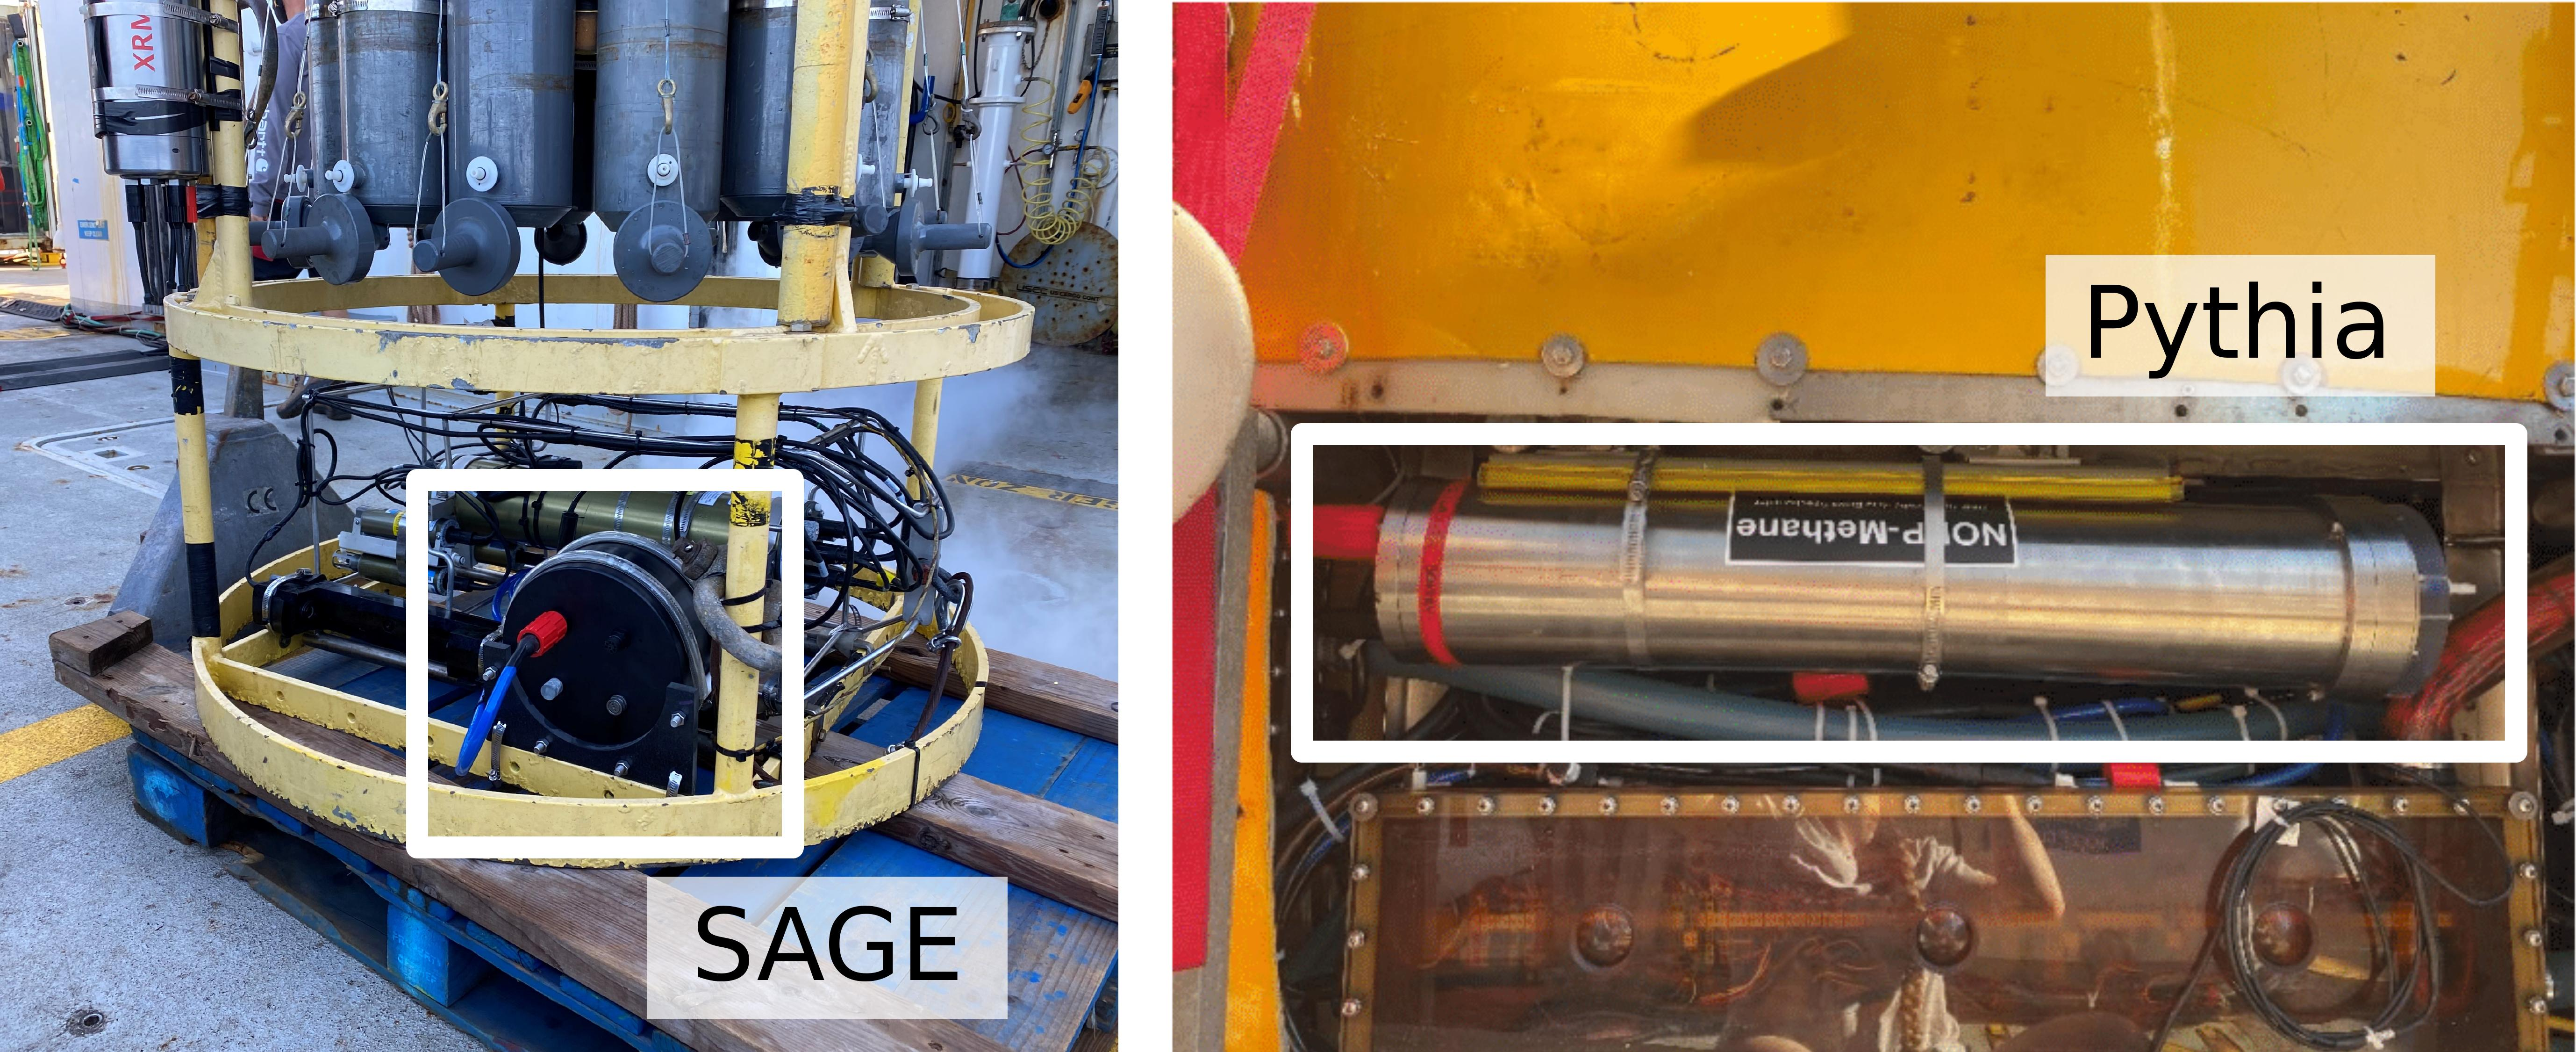
\includegraphics[width=\columnwidth]{figures/chap3_methane_sensor_mounting.jpg}
    \caption[Images of SAGE and Pythia methane instruments.]{\textbf{Images of the SAGE and Pythia methane instruments.} The SAGE and Pythia instruments were mounted on the rosette and AUV \emph{Sentry}, respectively.}
    \label{fig:sensor_mounting}
\end{figure}


\paragraph{SAGE}
\label{sec:sage}
SAGE is a dissolved gas sensing technology developed at the Woods Hole Oceanographic Institution (WHOI), and this expedition served as the first at-sea validation of the sensor's operation. SAGE technology has been previously described in \cite{kapit2021dissolved, kapit2021measurement}. Briefly, SAGE is based on infrared absorption spectroscopy performed on extracted gas from seawater via a gas permeable (and water impermeable) membrane. Once the gas enters the sensor, it fills a hollow-core optical fiber (HCF) which also guides light from a laser source tuned to measure the gas species of interest. The amount of target gas present is determined by measuring the amount of light absorption through the HCF using a photodetector. The prototype version of SAGE deployed on the research cruise was configured to measure methane in the range of 0-10,000 ppm. The resolution of the sensor was $<$1 ppm and the response time for the deployed configuration was approximately 12 minutes. For the scales of observations reported in this chapter (i.e., $<$2\% of the full scale of the observed signal), the instrument was minimally sensitive to temperature. SAGE is \SI{5.5}{\inch} long with a \SI{9}{\inch} outer diameter, and the power requirement was 7 W during this field deployment.

\paragraph{Pythia}
\label{sec:nopp}
Pythia is a novel deep-sea methane sensor developed utilizing real-time cavity ringdown spectroscopy (rt-CRDS) developed by WHOI~\autocite{michel2022gas} and Ring-IR Inc.~\autocite{Harb:12}, and capable of operating to \SI{4000}{\meter} depths. Pythia extracts dissolved gas from sea water using a large (\SI{113}{\centi\meter\squared}) surface area membrane. The extracted sample gas enters an optical cell where it is interrogated by a pulsed mid-infrared Quantum cascade laser (QCL). The laser light is absorbed by methane present in the cell, and the concentration of methane is determined by monitoring the pulsed ringdown signal from the cell using a mercury cadmium telluride (MCT) detector. While the response time of the sensor is slow, on the order of 35 minutes, the sensor is responsive to small ($<$2 ppm) changes in methane; the temperature sensitivity of Pythia has not yet been characterized. Pythia is ideally suited for long dives in environments in which changes to the methane concentration vary over long temporal and spatial scales. Details on the process for normalizing Pythia observations (which are strongly nonlinear and additionally require time correction) are provided in Appendix~\ref{app:perception:norm}. Pythia is \SI{24}{\inch} long with a \SI{4.5}{\inch} outer diameter, and was operated at a power range between 30-50 W during this field deployment.

\subsection{Analytical Procedure}
\label{sec:analytical}
Observations collected by sensors deployed on AUV \emph{Sentry}, including Pythia, were merged into a single dataframe using a common 1 Hz time reference; data were linearly interpolated onto this common time reference if they did not share an exact timestamp. With the exception of the derivative of ORP signal, all data for the purposes of visualization is smoothed using a centered rolling average over 5 minute intervals. Additionally, temperature, oxygen, and salinity measurements are normalized with respect to depth (as these quantities are anticipated to be functions of depth in the weakly stratified deep waters). Depth correction is performed by fitting a linear function to the average observation collected in \SI{20}{\meter} wide depth-bins, and computing the residuals of all data points with respect to this line (see Appendix~\ref{app:perception:depth} for plots of the linear functions). Rosette data is treated in the same fashion as \emph{Sentry} data. Down-cast and up-casts are removed from both \emph{Sentry} and rosette data streams for all visualizations.

\subsection{Transect Design and Execution}
AUV \emph{Sentry} and the rosette were deployed in the basin approximately \SI{16}{\kilo\meter} from the northern hydrothermal ridge structure, at (27.348152 N, 111.253108 W) with a course of \SI{295}{\degree} set to intersect the southern part of the ridge (Fig.~\ref{fig:bathy}). The \emph{Sentry} trackline was placed approximately 200-\SI{300}{\meter} north of the rosette to avoid any risk of entanglement. \emph{Sentry} was set in altitude hold mode, targeting \SI{120}{\meter} from the bottom (this places \emph{Sentry} at a depth of approximately 1750-\SI{1700}{\meter}, and at the top of its altitude-hold range). Rosette depth was targeted to be approximately 1650-\SI{1600}{\meter}, controlled primarily by the speed of the ship and length of the winch cable. These depths were designed based on an estimated model of the neutrally buoyant plume layer, as described in \cref{app:perception:model}. Leg 1 of the rosette trajectory was terminated at a planned stop at (27.393855 N, 111.364637 W), and Leg 2 was resumed at (27.460812 N, 111.527694 W); see Appendix~\ref{app:perception:niskin} for the schedule of bottle samples collected during Leg 2 presented in this manuscript. At the time of the transect, there were no known hydrothermal sites present over the sampling trajectory, save for the northern ridge. Hydrothermal vents in the southern basin were located approximately \SI{40}{\kilo\meter} further south from the transect starting location~\autocite{teske2016guaymas}.

\subsubsection{Modeling to Inform Transect Design}
\label{sec:afar_model}
The selection of heights for the rosette and AUV \emph{Sentry} was informed by a simple buoyancy model of expected plume characteristics on the ridge, and known operational constraints of AUV \emph{Sentry} (i.e., an absolute floor and ceiling of operation above the bottom). Using an adapted plume crossflow model developed by~\cite{tohidi2016highly} (see Appendix~\ref{app:perception:model} for more detailed information) with a nominal current crossflow value of \SI{0.1}{\meter\per\second}, vent temperature of \SI{340}{\celsius}, and estimated background seawater stratification as per~\cite{speer1989model}, a neutrally-buoyant layer was estimated to form between \SI{1570}{\meter} and \SI{1750}{\meter}. The depths for the rosette (1600-1650 m) and AUV \emph{Sentry} (1700-1750 m) were set given this information in order to target both the upper and lower estimated neutrally buoyant layer (NBL), respectively. The NBL was targeted to increase the likelihood of intersecting plume waters during the transect over a broad, multi-kilometer scope. This is in contrast with targeting the plume buoyant stem, which though significantly easier to distinguish from background seawater, may only have an expression on the order of several square meters.

\subsubsection{Real-Time Data Feedback and Watchstanding}
During the transect, data from the standard rosette sensors were available in near-real time at the watchstander station in the shipboard computer lab. This allowed watchstanders to monitor the depth of the rosette and relay requests to the winch operator on deck, and display the data on live-updating visualizers. AUV \emph{Sentry} relayed occasional data packets up to 128 bytes in length at a rate of approximately 0.01 Hz. These data packets were subsequently graphed on a computer monitor that was linked to the \emph{Sentry} network. A total of 600 messages with information about the standard science instruments on \emph{Sentry}, and 583 messages with information from the Pythia instrument were transferred during the transect.

\section{Results}
\label{sec:afar_results}

% Methane Instruments
\subsection{Methane Measured by Spectroscopic Instruments}
\label{sec:methane_results}
Elevated methane was observed over a spatial scale of several kilometers, significantly rising as both AUV \emph{Sentry} and the rosette approached the source of known hydrothermalism on the transect (Fig.~\ref{fig:methane_distance}). As both methane instruments used on this cruise were in active development, methane observations are reported as normalized values from 0 to 1. A normalized value of 0.5 is used as a conservative threshold for classifying elevated methane measurements. Pythia, mounted on \emph{Sentry}, reached and exceeded this threshold for elevated methane starting at approximately \SI{3}{\kilo\meter} from the hydrothermal reference point at (27.407489 N, 111.389893 W); SAGE, flying nearly \SI{50}{\meter} higher in the water column, reached this threshold starting \SI{1.5}{\kilo\meter} away. For a less conservative threshold of 0.3, these spatial detection points are reached 6.8 km and 2.2 km away, respectively. SAGE observed a sharp peak of methane just under \SI{1}{\kilo\meter} from the reference source, with rapid decline of observable methane soon after. In contrast, Pythia reached a methane peak essentially at the \SI{0}{\kilo\meter} reference point, and shows a gradual decline in methane as \emph{Sentry} descends into a graben just north of the hydrothermal ridge; the rosette was pulled from the water at the ridge. The difference in spatial detection patterns indicated by these instruments may be a function of the different sensor modalities/sensitivities, the natural structure of the neutrally-buoyant layer, and the relative position of the two platforms within it. 

\begin{figure}[h!]
    \centering
    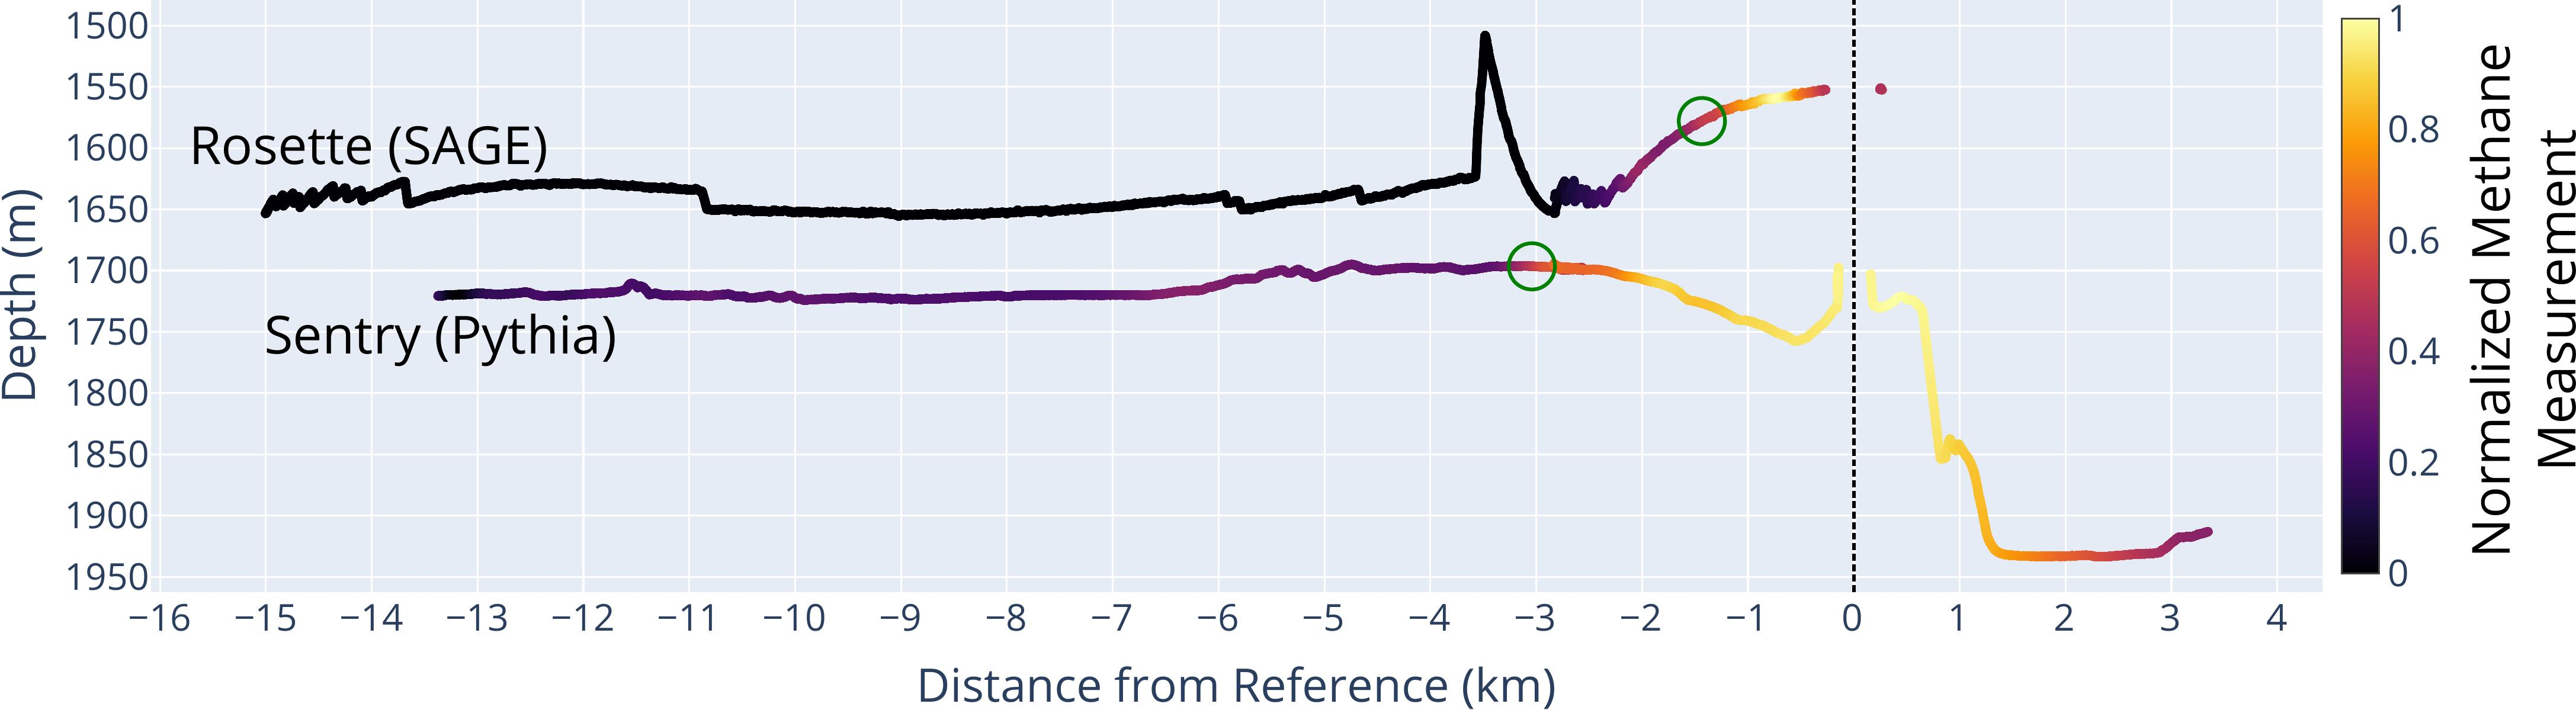
\includegraphics[width=1\columnwidth]{figures/chap3_methane_over_distance.jpg}
    \caption[Methane observations collected over the transect.]{\textbf{Methane observations collected over the transect.} Normalized methane values observed with both SAGE (rosette) and Pythia (\emph{Sentry}) over reference distance from (27.407489 N, 111.389893 W). The transect begins at the left of the plot and proceeds to the right. Strong methane anomalies, defined as points above a conservative threshold of 0.5 normalized values, are present starting \SI{3}{\kilo\meter} from the reference source as observed by Pythia, and \SI{1.5}{\kilo\meter} as observed by SAGE (open green circles).}
    \label{fig:methane_distance}
\end{figure}


% Methane + Ammonium
\subsection{Methane and Ammonium Measured with the Rosette}
Ammonium is a microbial energy source and reduced compound that is produced by the hydrothermal vents at Guaymas Basin. It is expected that ammonium and methane behavior in the basin will behave similarly, providing a ``check'' on the methane trends observed in methane bottle samples, and recorded by SAGE. Focusing primarily on Leg 2 of the rosette transect, there is a correspondence between methane and ammonium elevation in the approach to the hydrothermal ridge (Fig.~\ref{fig:bottles}). Methane samples processed directly from Niskin bottles as outlined in Sec.~\ref{sec:bottles} show a peak methane concentration of 3000-4000 nM (this range is associated with the extremes of calibrated extraction efficiencies valid for the equipment used), approximately \SI{0.75}{\kilo\meter} from the hydrothermal reference point. Ammonium tracks closely with methane, at 3-4 times smaller concentration, reaching a peak of approximately 1000 nM. 

Normalized methane observations by SAGE generally follow the trends shown by the bottle samples, similarly showing a spatial peak at \SI{0.75}{\kilo\meter}. However, by its nature, SAGE yields a significantly more resolved signal; a small, secondary peak is observed by SAGE at \SI{2}{\kilo\meter} from the reference point which is essentially missed by the bottle samples. Additionally, by virtue of operating continuously, there is no need for human interaction (unlike for processing bottle samples, which can require time-intensive \emph{ex situ} analysis). 

\begin{figure}[h!]
    \centering
    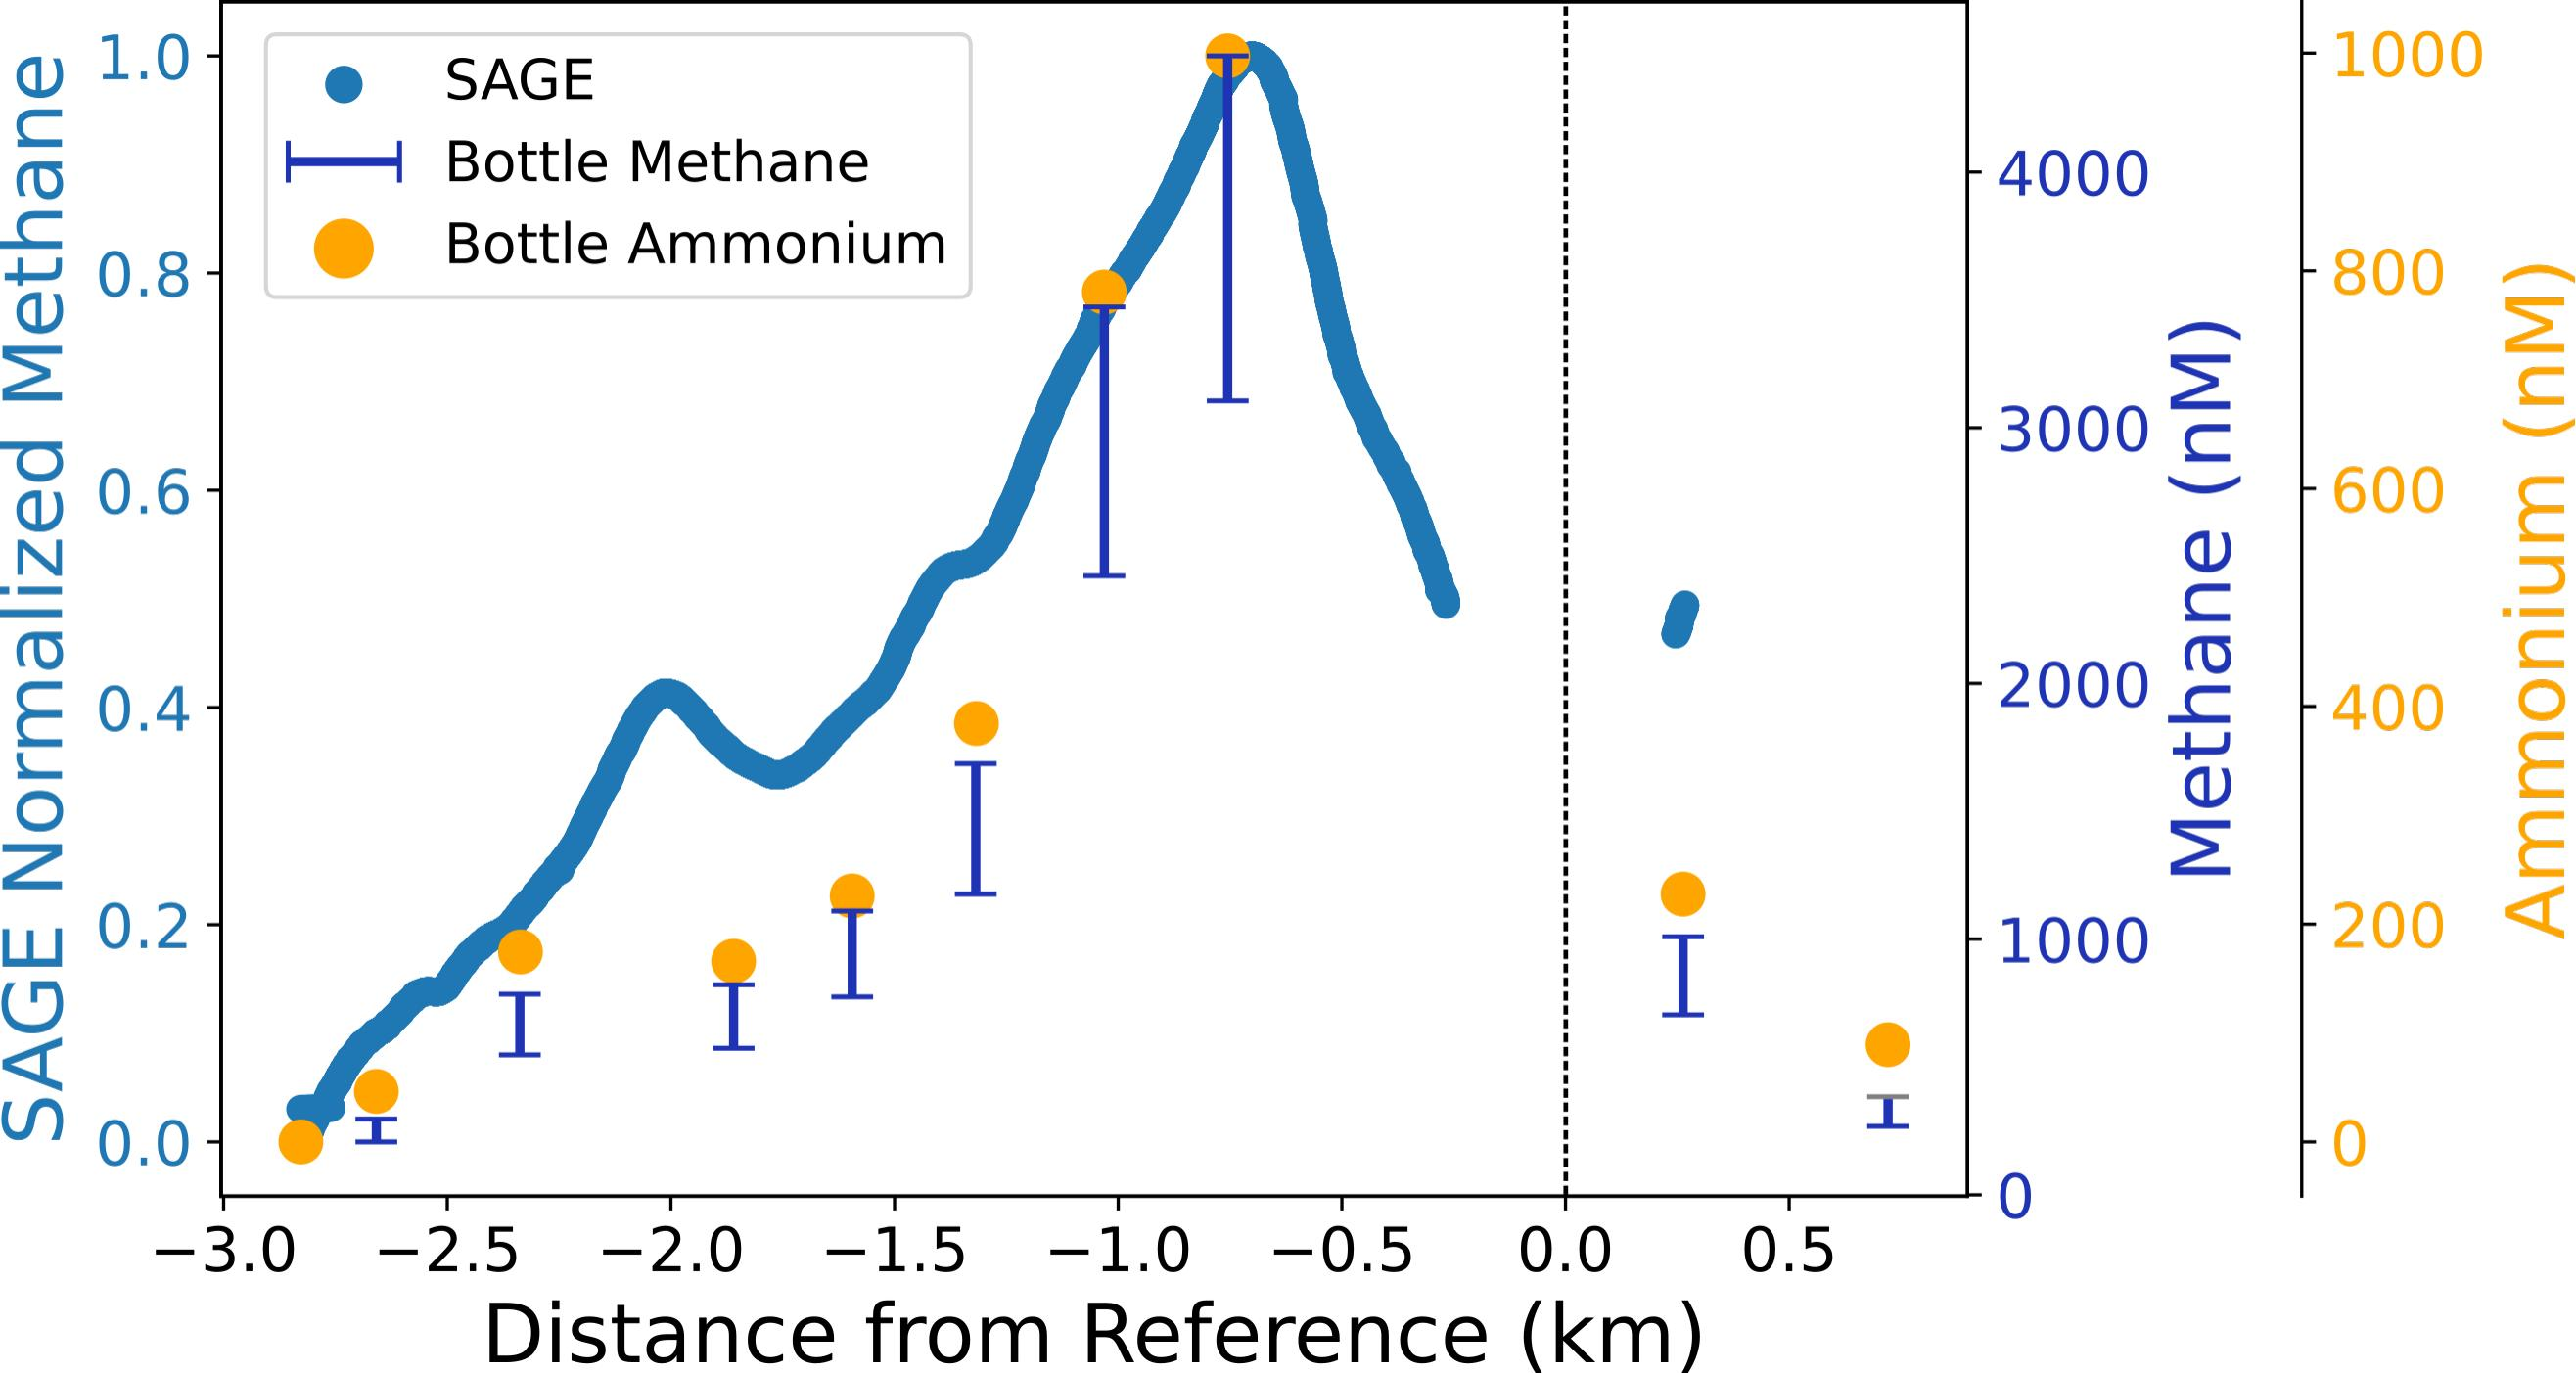
\includegraphics[width=\columnwidth]{figures/chap3_bottle_norm.jpg}
    \caption[Methane observations compared to ammonium concentrations.]{\textbf{Methane observations compared to ammonium concentrations.} Normalized methane measurements by SAGE plotted with methane measurements taken from Niskin bottle samples (as measured by DGEU/GGA equipment) and ammonium measurements. Bottle methane measurements are reported as a range to reflect sensitivity of the measurement procedure to a calibrated extraction efficiency. All measurements trend towards a peak observation of methane and ammonium \SI{0.75}{\kilo\meter} from the reference source. SAGE additionally observes a secondary peak approximately \SI{2}{\kilo\meter} from the source, which is essentially missed by the bottle sample schedule.}
    \label{fig:bottles}
\end{figure}


% Turbidity
\subsection{Turbidity}
\label{sec:turbidity_results}
Turbidity is a commonly used indicator for detecting hydrothermalism from smoking vents; particulate matter produced by smoking vents can remain suspended in the neutrally buoyant layer, acting as a non-conservative tracer for hydrothermalism~\autocite{feely1992tracking}. In the Guaymas Basin, suspended particulates have been shown to be composed of metals like iron, aluminum, and manganese~\autocite{scholz2019shelf} and are primarily mixed into bottom waters from hydrothermal activity. Here, turbidity measurements are reported as normalized values to make direct comparison between the platforms straightforward; in absolute terms, the transmissometer on the rosette reported beam attenuation values between 0-0.2 and the OBS on \emph{Sentry} observed backscatter values between 0.08-0.14. The OBS on \emph{Sentry} encountered an error from the beginning of the dive, potentially caused by a persistent air bubble, until approximately \SI{4.5}{\kilo\meter} from the the ridge reference point; these early measurements are omitted. 

Elevated turbidity (defined by a conservative threshold of 0.5 in the normalized data) was observed with the transmissometer on the rosette starting approximately \SI{2.2}{\kilo\meter} from the reference source and \SI{3.3}{\kilo\meter} with the OBS on \emph{Sentry} (Fig.~\ref{fig:turbidity_distance}). Even with a less conservative threshold (0.3) these detection points only slightly improve to 2.5 km and 3.4 km respectively. With \emph{Sentry}, a rapid decline in turbidity within tens of meters west of the source reference (positive distance in Fig.~\ref{fig:turbidity_distance}) is observed. This may be indicative of the direction of prevailing crossflow (southeast) in the basin, which would directionally bend a buoyant plume stem and advect the neutrally buoyant layer.

\begin{figure}[h!]
    \centering
    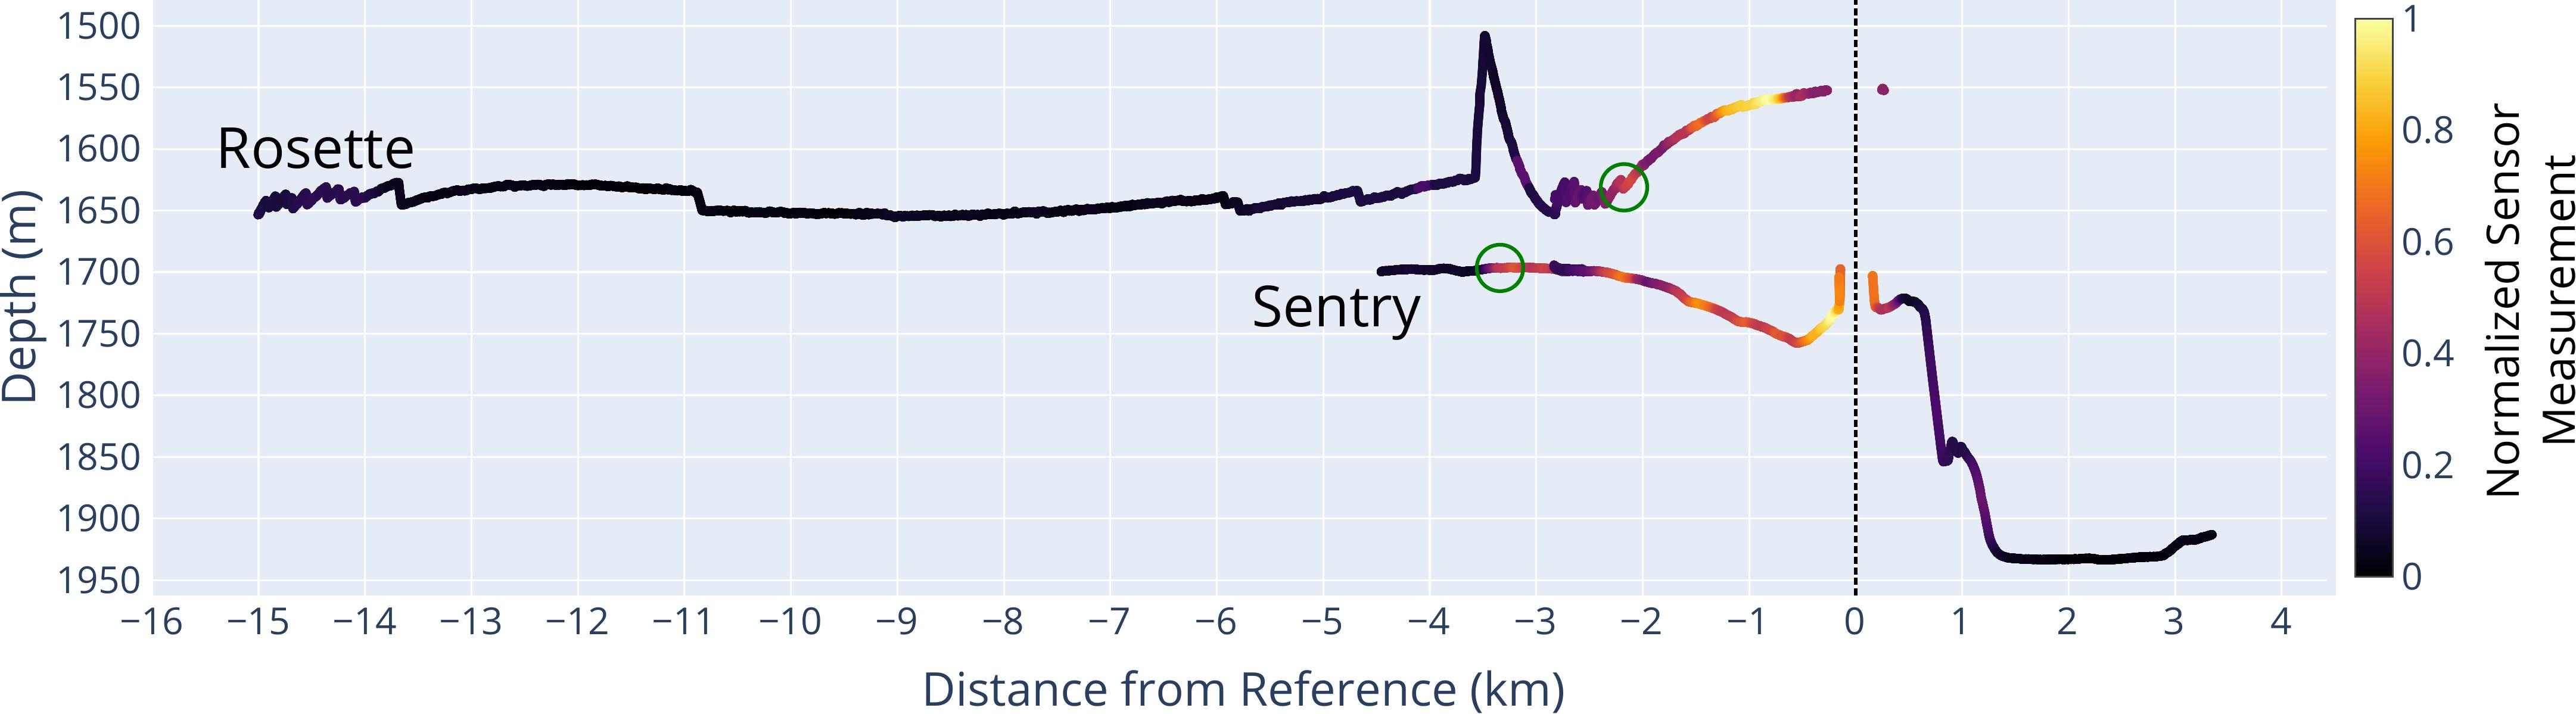
\includegraphics[width=\columnwidth]{figures/chap3_turbidity_over_distance.jpg}
    \caption[Turbidity measurements collected during transect.]{\textbf{Turbidity measurements collected during the transect.} Turbidity observed as beam attenuation on the rosette transmissometer and optical backscatter on AUV \emph{Sentry} instruments. \emph{Sentry} encountered a sensor error until approximately \SI{4.5}{\kilo\meter} from the ridge reference point. After this point, elevated turbidity is detectable throughout the dive, with significant elevations within \SI{3.3}{\kilo\meter} east of the ridge reference point, dissipating within tens of meters to the west. Elevated turbidity is observed by the rosette \SI{2.2}{\kilo\meter} from the ridge reference point to the east.}
    \label{fig:turbidity_distance}
\end{figure}


% ORP
\subsection{Oxidation Reduction Potential}
AUV \emph{Sentry} carries an ORP sensor; there was no comparable sensor on the rosette. ORP sensors are commonly used in hydrothermal plume hunting, and can be a strong indicator of recently emitted hydrothermal fluids. The derivative of ORP (noted here as dORPdt) is particularly used, in which negative dORPdt values typically indicate transition from background water into hydrothermal fluid. During the transect, only one significant dORPdt deviation was observed, within \SI{200}{\meter} from the ridge reference point (Fig.~\ref{fig:orp_distance}). 

\begin{figure}[t!]
    \centering
    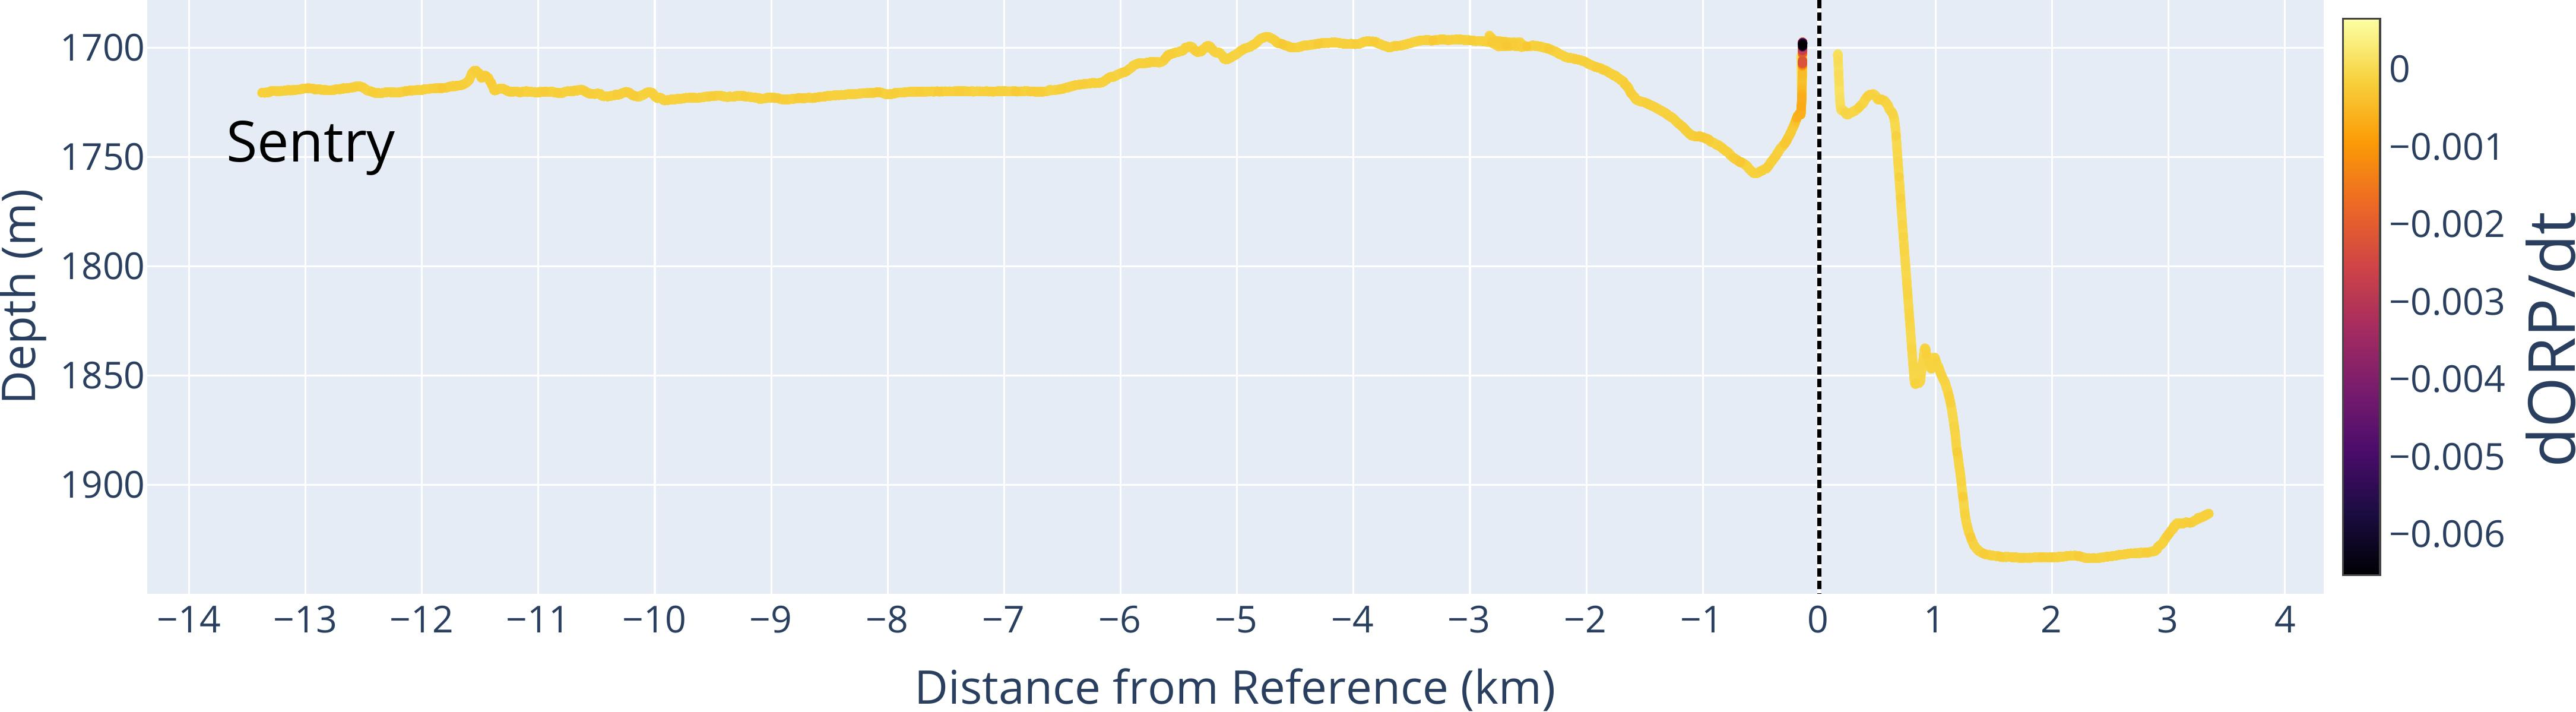
\includegraphics[width=\columnwidth]{figures/chap3_orp_over_distance.jpg}
    \caption[Oxidation-reduction potential measurements collected during transect.]{\textbf{Oxidation-reduction potential measurements collected during transect.} The derivative of ORP observed by data collected on AUV \emph{Sentry}. Negative slopes are indicative of entering hydrothermal fluids. Only one region of the transect demonstrated a significant reaction to ORP, within \SI{200}{\meter} of the reference point.}
    \label{fig:orp_distance}
\end{figure}

% Temp, Salt, O2
\subsection{Temperature, Salinity, and Oxygen}
\label{sec:o2_temp_salt}
Temperature, salinity, and oxygen are expected to be weakly stratified in deep ocean waters, however fluids from hydrothermalism should register as anomalies when present. The magnitude of valid anomalies (i.e., anomalies that positively identify fluids impacted by hydrothermalism) can be exceedingly small; temperature at a vent can be hundreds of degrees Celsius, but anomalies in the water column on the spatial order of only \SI{10}{\meter} can be measured as single degrees, and within a neutrally-buoyant plume on the order of hundreds of meters from the source, only register a few hundredths of a degree~\autocite{yoerger2007autonomous}. 

Temperature, salinity, and oxygen anomalies are computed according to the process described in Sec.~\ref{sec:analytical} and the results are shown in Fig.~\ref{fig:o2_temp_salt}. Salinity anomalies, although apparently coherent, are reported within the empirical sensor noise for the CTD instruments on both the rosette and \emph{Sentry}. Temperature anomalies on the scale of hundredths of a degree are observed throughout the transect, with two key regions of high temperature anomaly, one located 6-12 km from the reference source, and the other within 3 km of the source. Both the rosette and \emph{Sentry} observe these regions; with \emph{Sentry} observing the first anomaly in a narrower margin between 8-11 km from the reference source. The first region of positive temperature anomaly closely corresponds with marginally fresher water; whereas the region of higher temperature anomaly near the source is not consistently matched in salinity (the rosette observes more salinity content, whereas \emph{Sentry} observes neutral or slightly less salinity content). Oxygen is reported as nominal or slightly depleted within the regions of notable temperature and salinity anomaly.

\begin{figure}[h!]
    \centering
    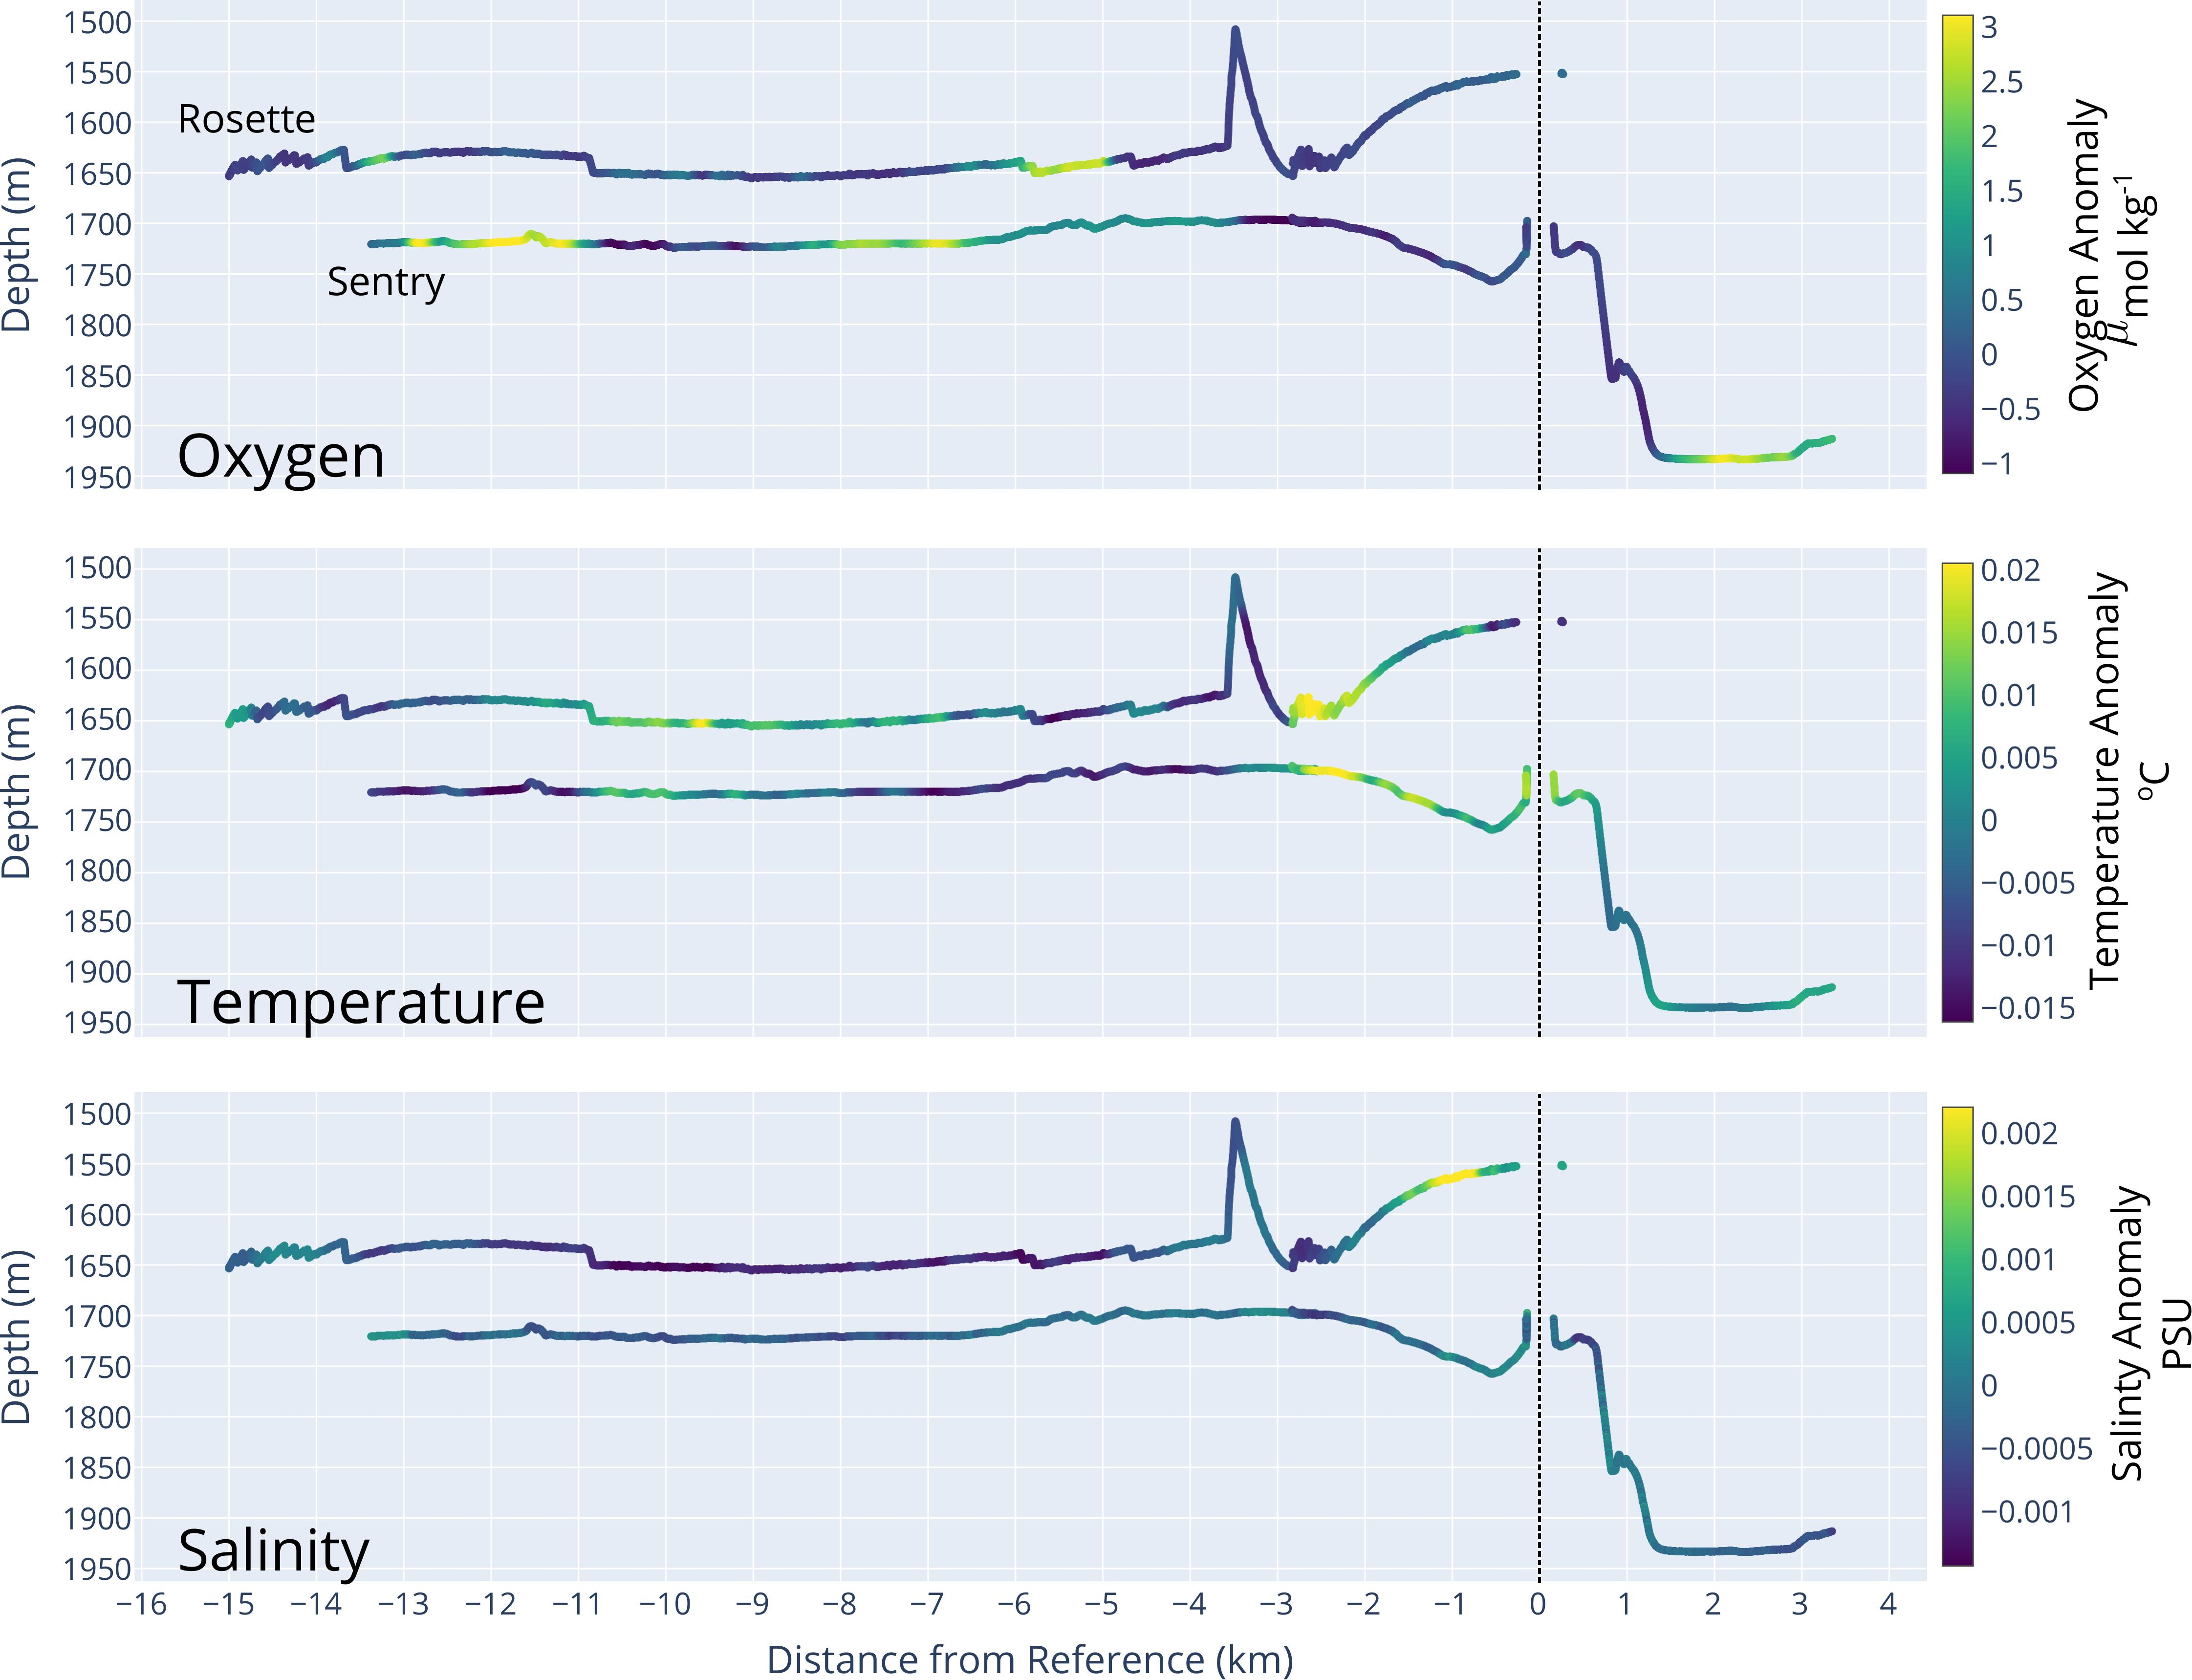
\includegraphics[width=1\columnwidth]{figures/chap3_o2_temp_salt_over_distance.jpg}
    \caption[Depth-corrected oxygen, temperature, and salinity measurements collected during transect.]{\textbf{Depth-corrected oxygen, temperature, and salinity over reference distance.} Two notable regions of high temperature deviation from expected temperature are observed between 6-12 km (rosette; 8-11 km by \emph{Sentry}) and within 3 km of the reference source. The first region of temperature anomaly is closely matched with fresher salinity measurements; whereas salinity is measured as marginally higher near the reference source by the rosette CTD and nominal or lower by the \emph{Sentry} CTD. In both regions, oxygen is nominal or slightly depleted, with regions of notably elevated oxygen at the boundary of these regions.}
    \label{fig:o2_temp_salt}
\end{figure}

The first region of interest, far afield from the plume reference point, appears coherent and has similar detection qualities to the near-reference region; however, given the typical expectation of temperature dissipation from hydrothermal sources, it would be surprising if this first region were connected with hydrothermalism. The shape of the warm, slightly fresher and oxygen depleted intrusion (laterally broad higher in the water column, and appearing to narrow based on the observations taken by the rosette and \emph{Sentry} approximately 50 m offset in altitude) also does not follow expected patterns in a neutrally buoyant plume layer. Lack of significant methane and turbidity observations in this same region, as presented in Sec.~\ref{sec:methane_results} and Sec.~\ref{sec:turbidity_results} respectively, additionally casts doubt on hydrothermalism as a driver for this anomaly. Water mass mixing between the bottom waters, largely sourced from Pacific Deep Waters and the Pacific Intermediate Waters~\autocite{bray1988water} may be an alternative explanation, but is out of scope for this study to investigate. 


\section{Discussion}

\subsection{Sensor Cross-Correlations}
\label{sec:correl}
Successfully detecting hydrothermalism in the deep ocean is a significant challenge, and detection may be most effective using a combination and corroboration of anomalies across multiple sensor inputs~\autocite{jakuba2007stochastic}. Here, the cross-correlation between sensors mounted on each of the platforms is investigated. Both a global and rolling Pearson correlation coefficient were computed, showing overall correlation trends and situation dependent correlation, respectively.

Fig.~\ref{fig:global_corr} shows the global correlation among sensors mounted on the rosette individually over Leg 1 and Leg 2, in addition to sensors mounted on \emph{Sentry}. In the absence of significant geochemical features in a target environment, it is expected that no or only weak correlation will be computed globally, as individual sensor noise (which is independent) will dominate the computation; when geochemical structure is present in the environment, it is expected that weak to strong global correlation will be computed as the environment is imposing a (shared) signal across at least a subset of sensors. This is well illustrated by the cross-correlation matrices for the rosette legs, with global coefficients for Leg 1 reporting no correlation between sensors save for a slightly negative correlation between temperature and oxygen, and for Leg 2 reporting weak to strong correlations between all sensors, with notably strong positive correlation between turbidity and methane. Interestingly, in Leg 2 a negative correlation is reported between temperature and methane, and a positive correlation is measured between methane and oxygen measurements. This runs directly counter to expectations; and also counter with the relationships observed by \emph{Sentry} which marks relationships between methane and temperature as positively correlated, and between methane and oxygen as negatively correlated. 

\begin{figure}[h!]
    \centering
    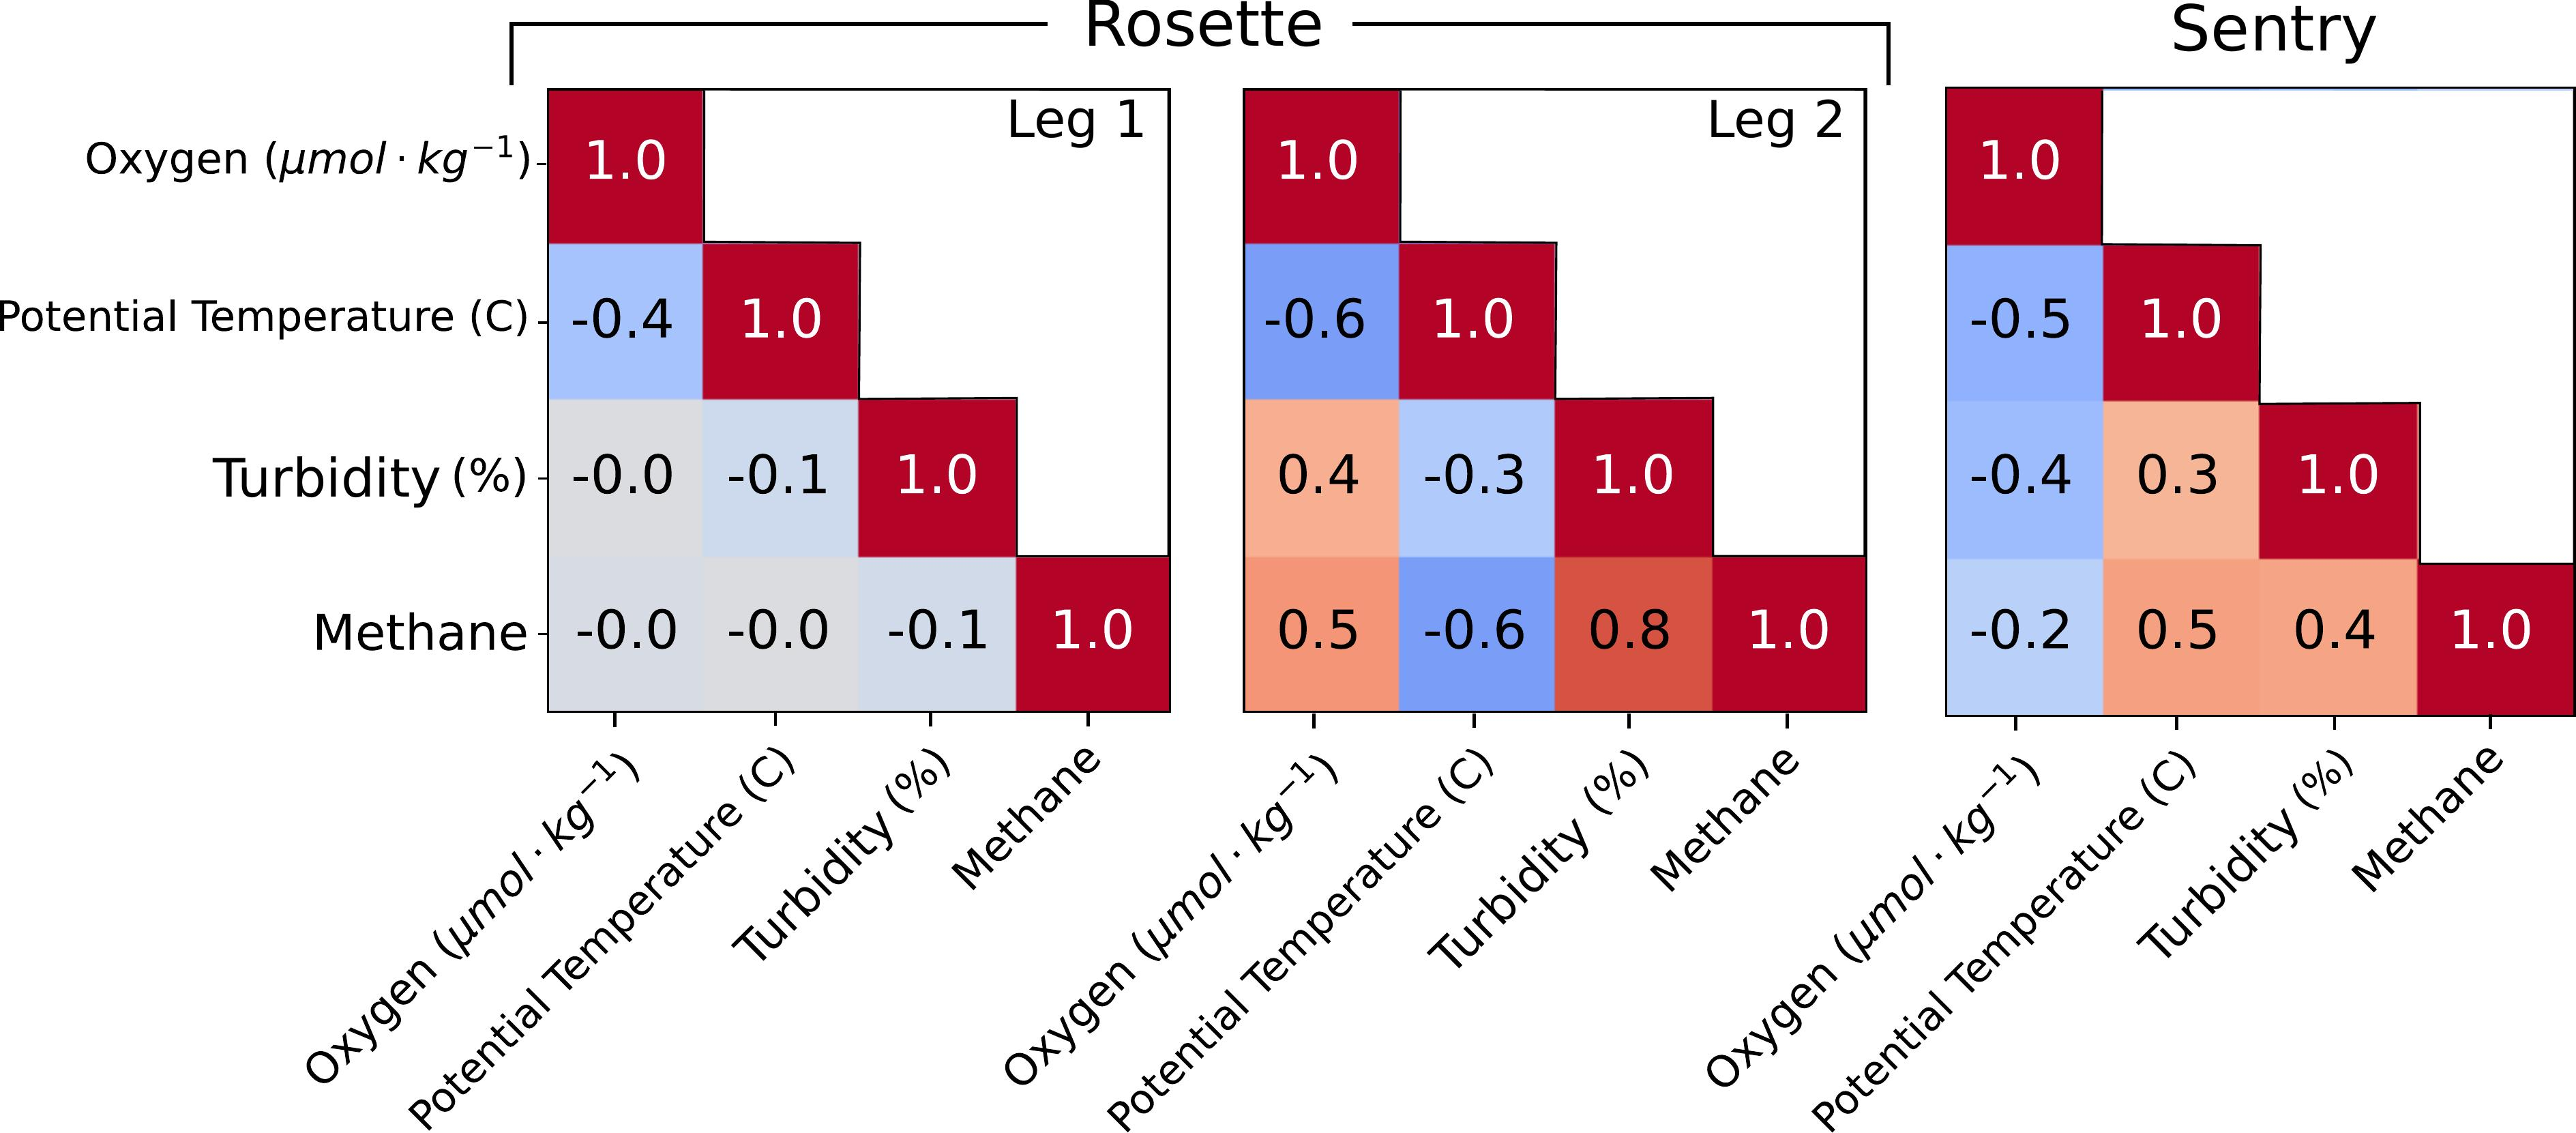
\includegraphics[width=0.9\columnwidth]{figures/chap3_all_global_corr.jpg}
    \caption[Global Pearson correlation coefficients between sensors mounted on the rosette and \Sentry.]{\textbf{Global Pearson correlation coefficient between sensors mounted on the rosette and \emph{Sentry}.} Correlation differences between Leg 1 (far from the reference point) and Leg 2 (near the reference point) are indicative of different sensor correlation behaviors with respect to ambient seawater conditions and hydrothermal fluid interception. \emph{Sentry} correlation coefficients reflect an expected relationship between temperature and methane (positive), methane and oxygen (negative), and turbidity and methane (positive) that may be stereotypically associated with hydrothermal fluids. In contrast, the Leg 2 rosette correlation factors do not meet this expectation, despite showing strong overall correlative structure.}
    \label{fig:global_corr}
\end{figure}

The difference between correlative behaviors between the rosette legs, and also between the platforms generally, motivates a finer study of correlation. Fig.~\ref{fig:rosette_local} shows a rolling correlation coefficient computed over a window of 30 minutes for the rosette. Computing local cross-correlations with respect to time, rather than distance, is mathematically more sound\footnote{In the sense that samples are regularly sampled in time, but irregularly sampled in space.}, and also aligns directly with how cross-correlative monitoring may be used during live exploration missions. Using the correlative ``micro-structure'' of rolling coefficients shows regions of possible interest that are greater than nominal (uncorrelated structure). Looking first at the rosette information, Leg 1 nominal correlation early in the transect is weak or non-existent between most sensors, with exception for oxygen and temperature at around 2:00. Additionally, a coherent region from 04:00-05:00 shows a negative correlation between temperature and turbidity, and positive correlation between temperature and oxygen. In Leg 2, overall more strong, pronounced correlations between sensors are observed, with a distinct period centered in the hour around 10:00 in which correlation between temperature and methane, temperature and turbidity, oxygen and methane, and oxygen and turbidity appear to ``flip'' compared to the periods of time directly before and after this period, potentially indicating a significant anomalous feature. This time period is well aligned with the spatial proximity of the rosette with the reference source.

\begin{figure}[h!]
    \centering
    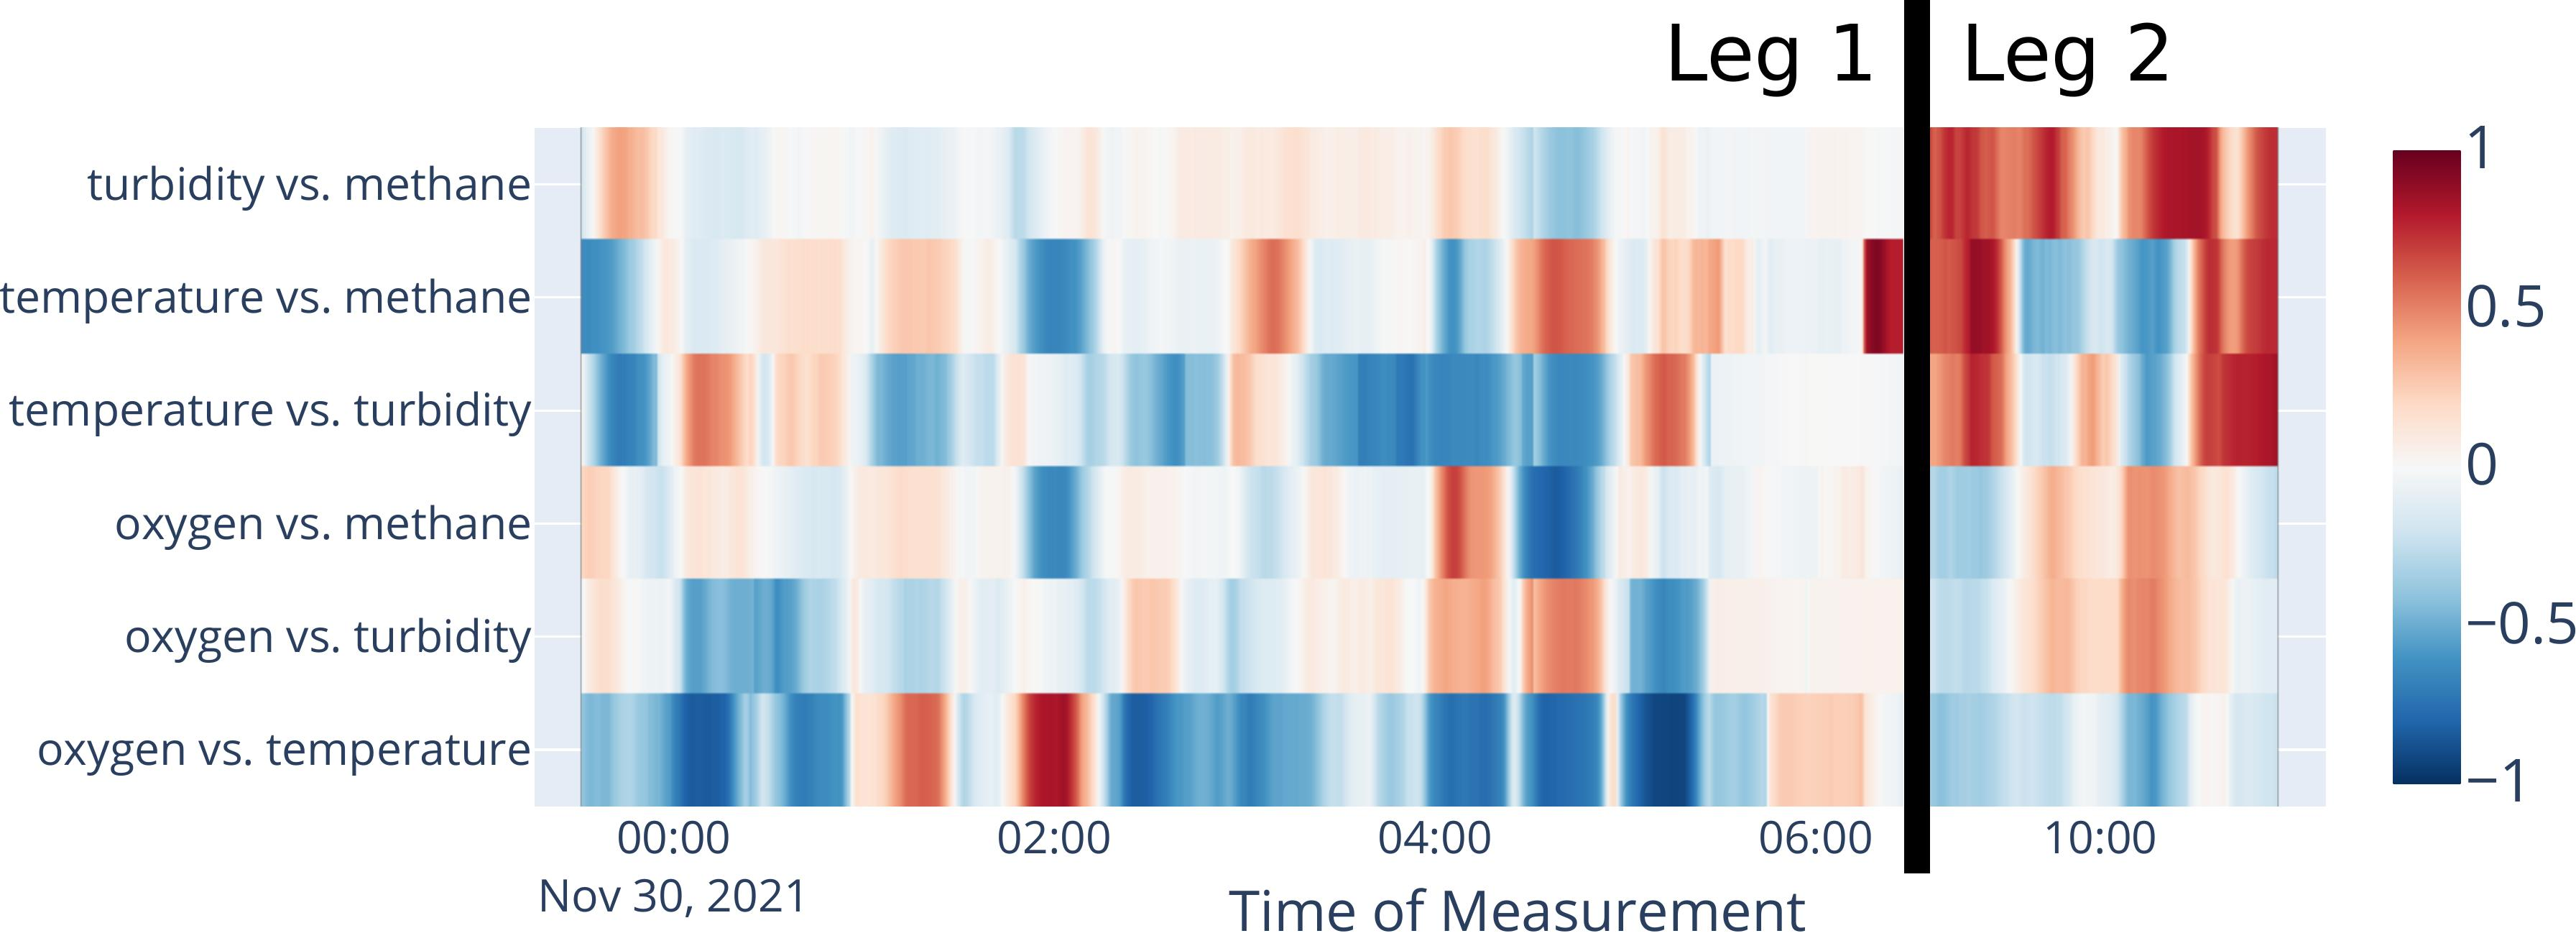
\includegraphics[width=\columnwidth]{figures/chap3_rosette_local_corr_all.jpg}
    \caption[Local (rolling) Pearson correlation coefficients for rosette mounted instruments.]{\textbf{Local (rolling) Pearson correlation coefficients between sensors mounted on the rosette over 30 minute windows.} Several regions of interest at 2:00 (strong temperature-oxygen correlation), 4:00-5:00 (notably coherent region of stronger correlation across multiple sensors), and during Leg 2 (near the venting source) can be picked out and may indicate anomalous water masses.}
    \label{fig:rosette_local}
\end{figure}

Local correlation trends during the \emph{Sentry} transect are reported in Fig.~\ref{fig:sentry_local}, and show an intense relationship between oxygen and temperature throughout the dive, with most of the transect reporting a strong negative correlation, save for two regions of positive correlation at 08:00 and again at 11:00. This strong relationship is also reflected in the relationships of temperature and oxygen with methane, being nearly correlative mirrors with respect to methane. During periods in which the turbidity sensor was operational, a gradual correlative ``flip'' and intensity increase in correlation between turbidity and oxygen around 11:00 may indicate a structured water mass. This time stamp agrees with the spatial proximity of \emph{Sentry} with the reference source.

\begin{figure}[h!]
    \centering
    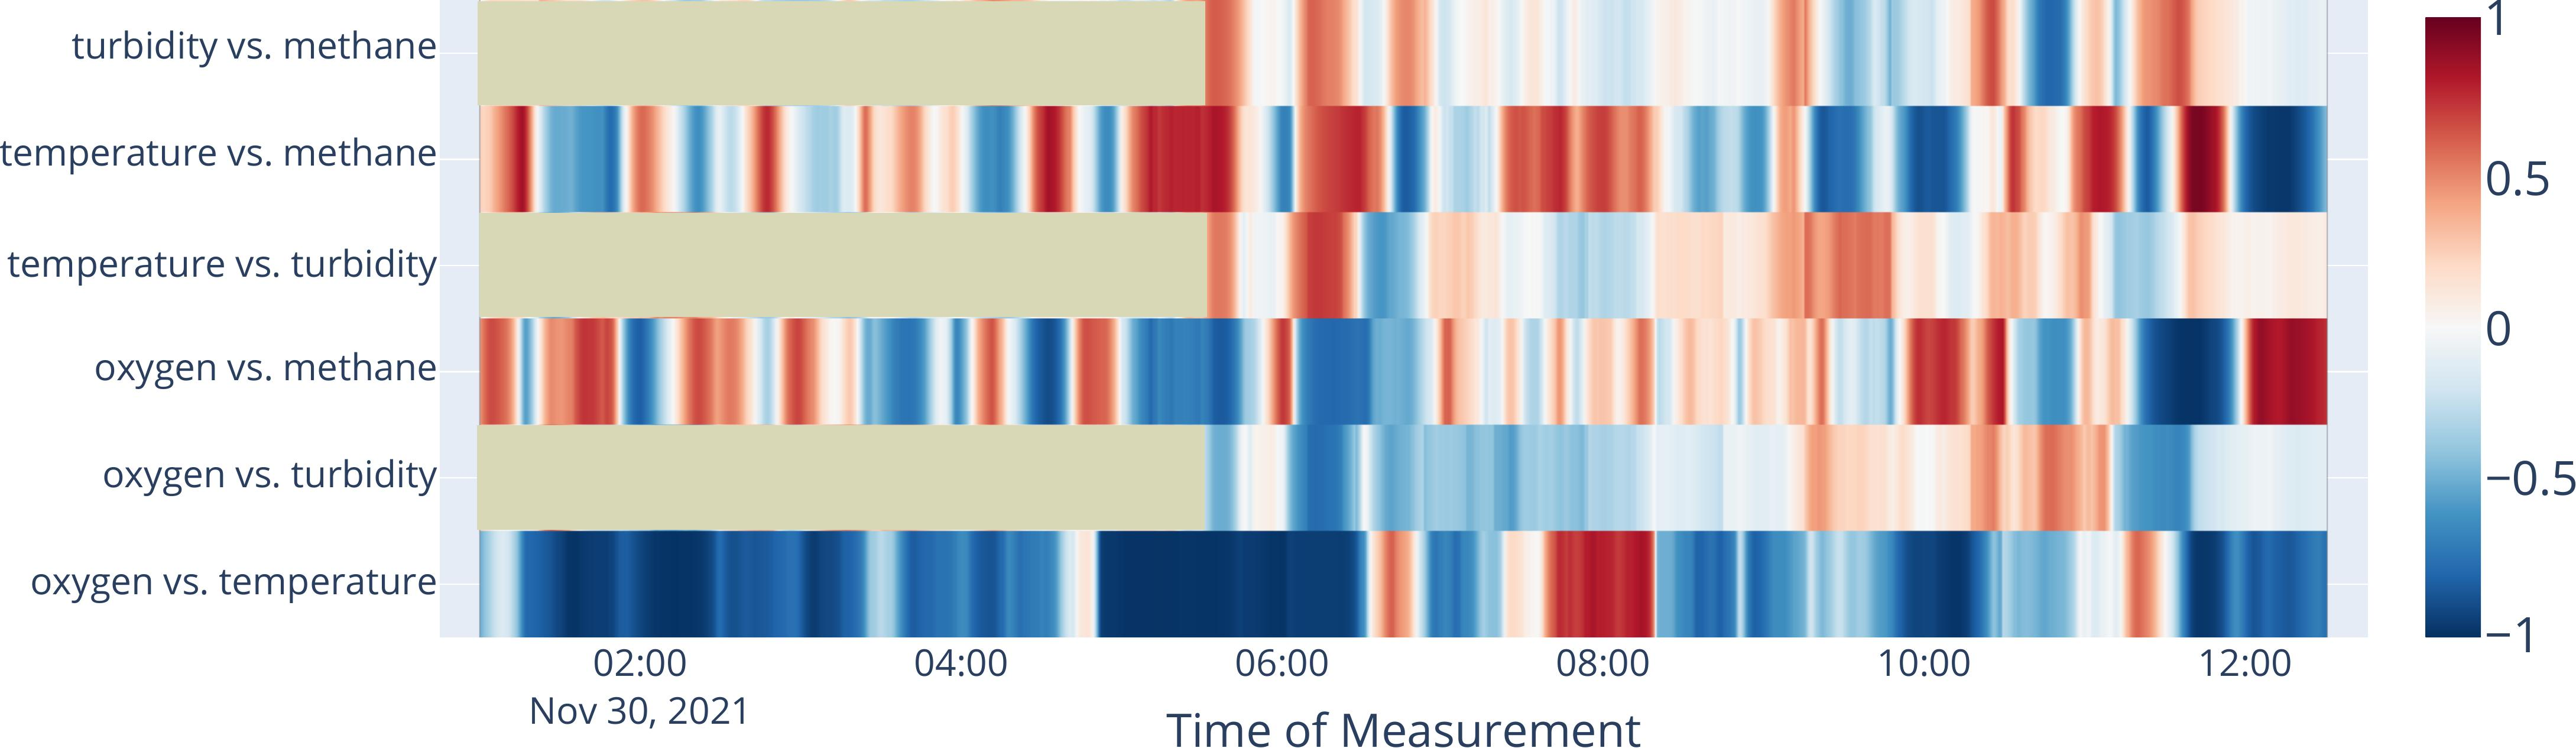
\includegraphics[width=1\columnwidth]{figures/chap3_sentry_local_corr_all.jpg}
    \caption[Local (rolling) Pearson correlation coefficients for AUV \Sentry mounted instruments.]{\textbf{Local (rolling) Pearson correlation coefficient between sensors mounted on AUV \emph{Sentry} over 30 minute windows.} Temperature and oxygen are strongly negatively correlated throughout the dive, with the exception of 08:00 and 11:00. For times in which the turbidity sensor was operational, the oxygen-turbidity correlative relationship slowly flips from negative to positive, with a peak positive correlation at 11:00. 11:00 agrees with the time that \Sentry was near the reference source vent.}
    \label{fig:sentry_local}
\end{figure}

Correlation alone is not sufficient evidence for the presence of hydrothermal fluids. For instance, some of the coherent regions of positive or negative correlation with methane any time during Leg 1, or early in the \emph{Sentry} transect, are misleading, as the overall methane content of the water was exceedingly small or essentially background. Rolling correlations, coupled with absolute thresholds as reported in \cref{sec:afar_results}, may together be useful tools for indicating transition into new water masses, their absolute properties of which could be used to more closely classify the types of water masses. This correlative study also demonstrates that correlations in expectation (e.g., temperature and methane being positively correlated in hydrothermal fluid) may be reductive assumptions of the complexities of plume evolution within a water column, supporting similar findings e.g., by~\cite{cowen2002methane}. For instance, aging plume waters in the neutrally buoyant layer may long have settled to a temperature indistinguishable from background, but still be particulate and possibly gas rich. This motivates additional study of the ``classes'' of hydrothermal fluids and their classifying characteristics, which could in turn be used to support studies of microbial evolution and nutrient consumption in plume fluids, or sediment and particulate transport modeling.

\subsection{Hydrothermalism Detection via Time-Series Regimes}
As indicated by Sec.~\ref{sec:correl}, changes in correlative \emph{structure} may be a more useful signal than absolute correlation alone. This notion can be codified as regime changes, which detect inflection points for which a series of observations collected in time may change in typical value, oscillation frequency, or pattern. Here, regime changes are computed over 30 minute detection windows using linearly penalized segmentation \autocite{killick2012optimal} (PELT) as implemented in the \verb|ruptures| Python library \autocite{truong2020selective} with a radial basis function detection kernel.
PELT is a linear-time offline algorithm for selecting changepoints that incrementally performs binary segmentation on a time-series (based on a cost function defined by the detection window and basis function) until all segments are self-consistent; these segments are regimes. In the included figures, we visualize regimes using alternating red and blue color blocks.

In Fig.~\ref{fig:rosette_regimes} regimes across the entire rosette transect over multiple sensors is illustrated. One initial observation is that the water-mixing anomaly that occurs early in the transect (Sec.~\ref{sec:o2_temp_salt}) appears to be detected as regime changes in potential temperature, oxygen, and even a correspondence in lowered beam attenuation. Similarly, regime changes in turbidity and methane are early indicators of significant elevation of both of these factors as the rosette intersects with hydrothermal fluids later in the transect. Interestingly, a regime change in oxygen and temperature is evident immediately following the first small peak in methane and turbidity in the absolute measurement data. These peaks, in addition to these regime changes, may together be indicative of mixing plume sources from other hydrothermal vents located along the ridge (that must travel further than fluids from our reference point) or the mixing of aging plume waters with more recently emitted fluids.

\begin{figure}[h!]
    \centering
    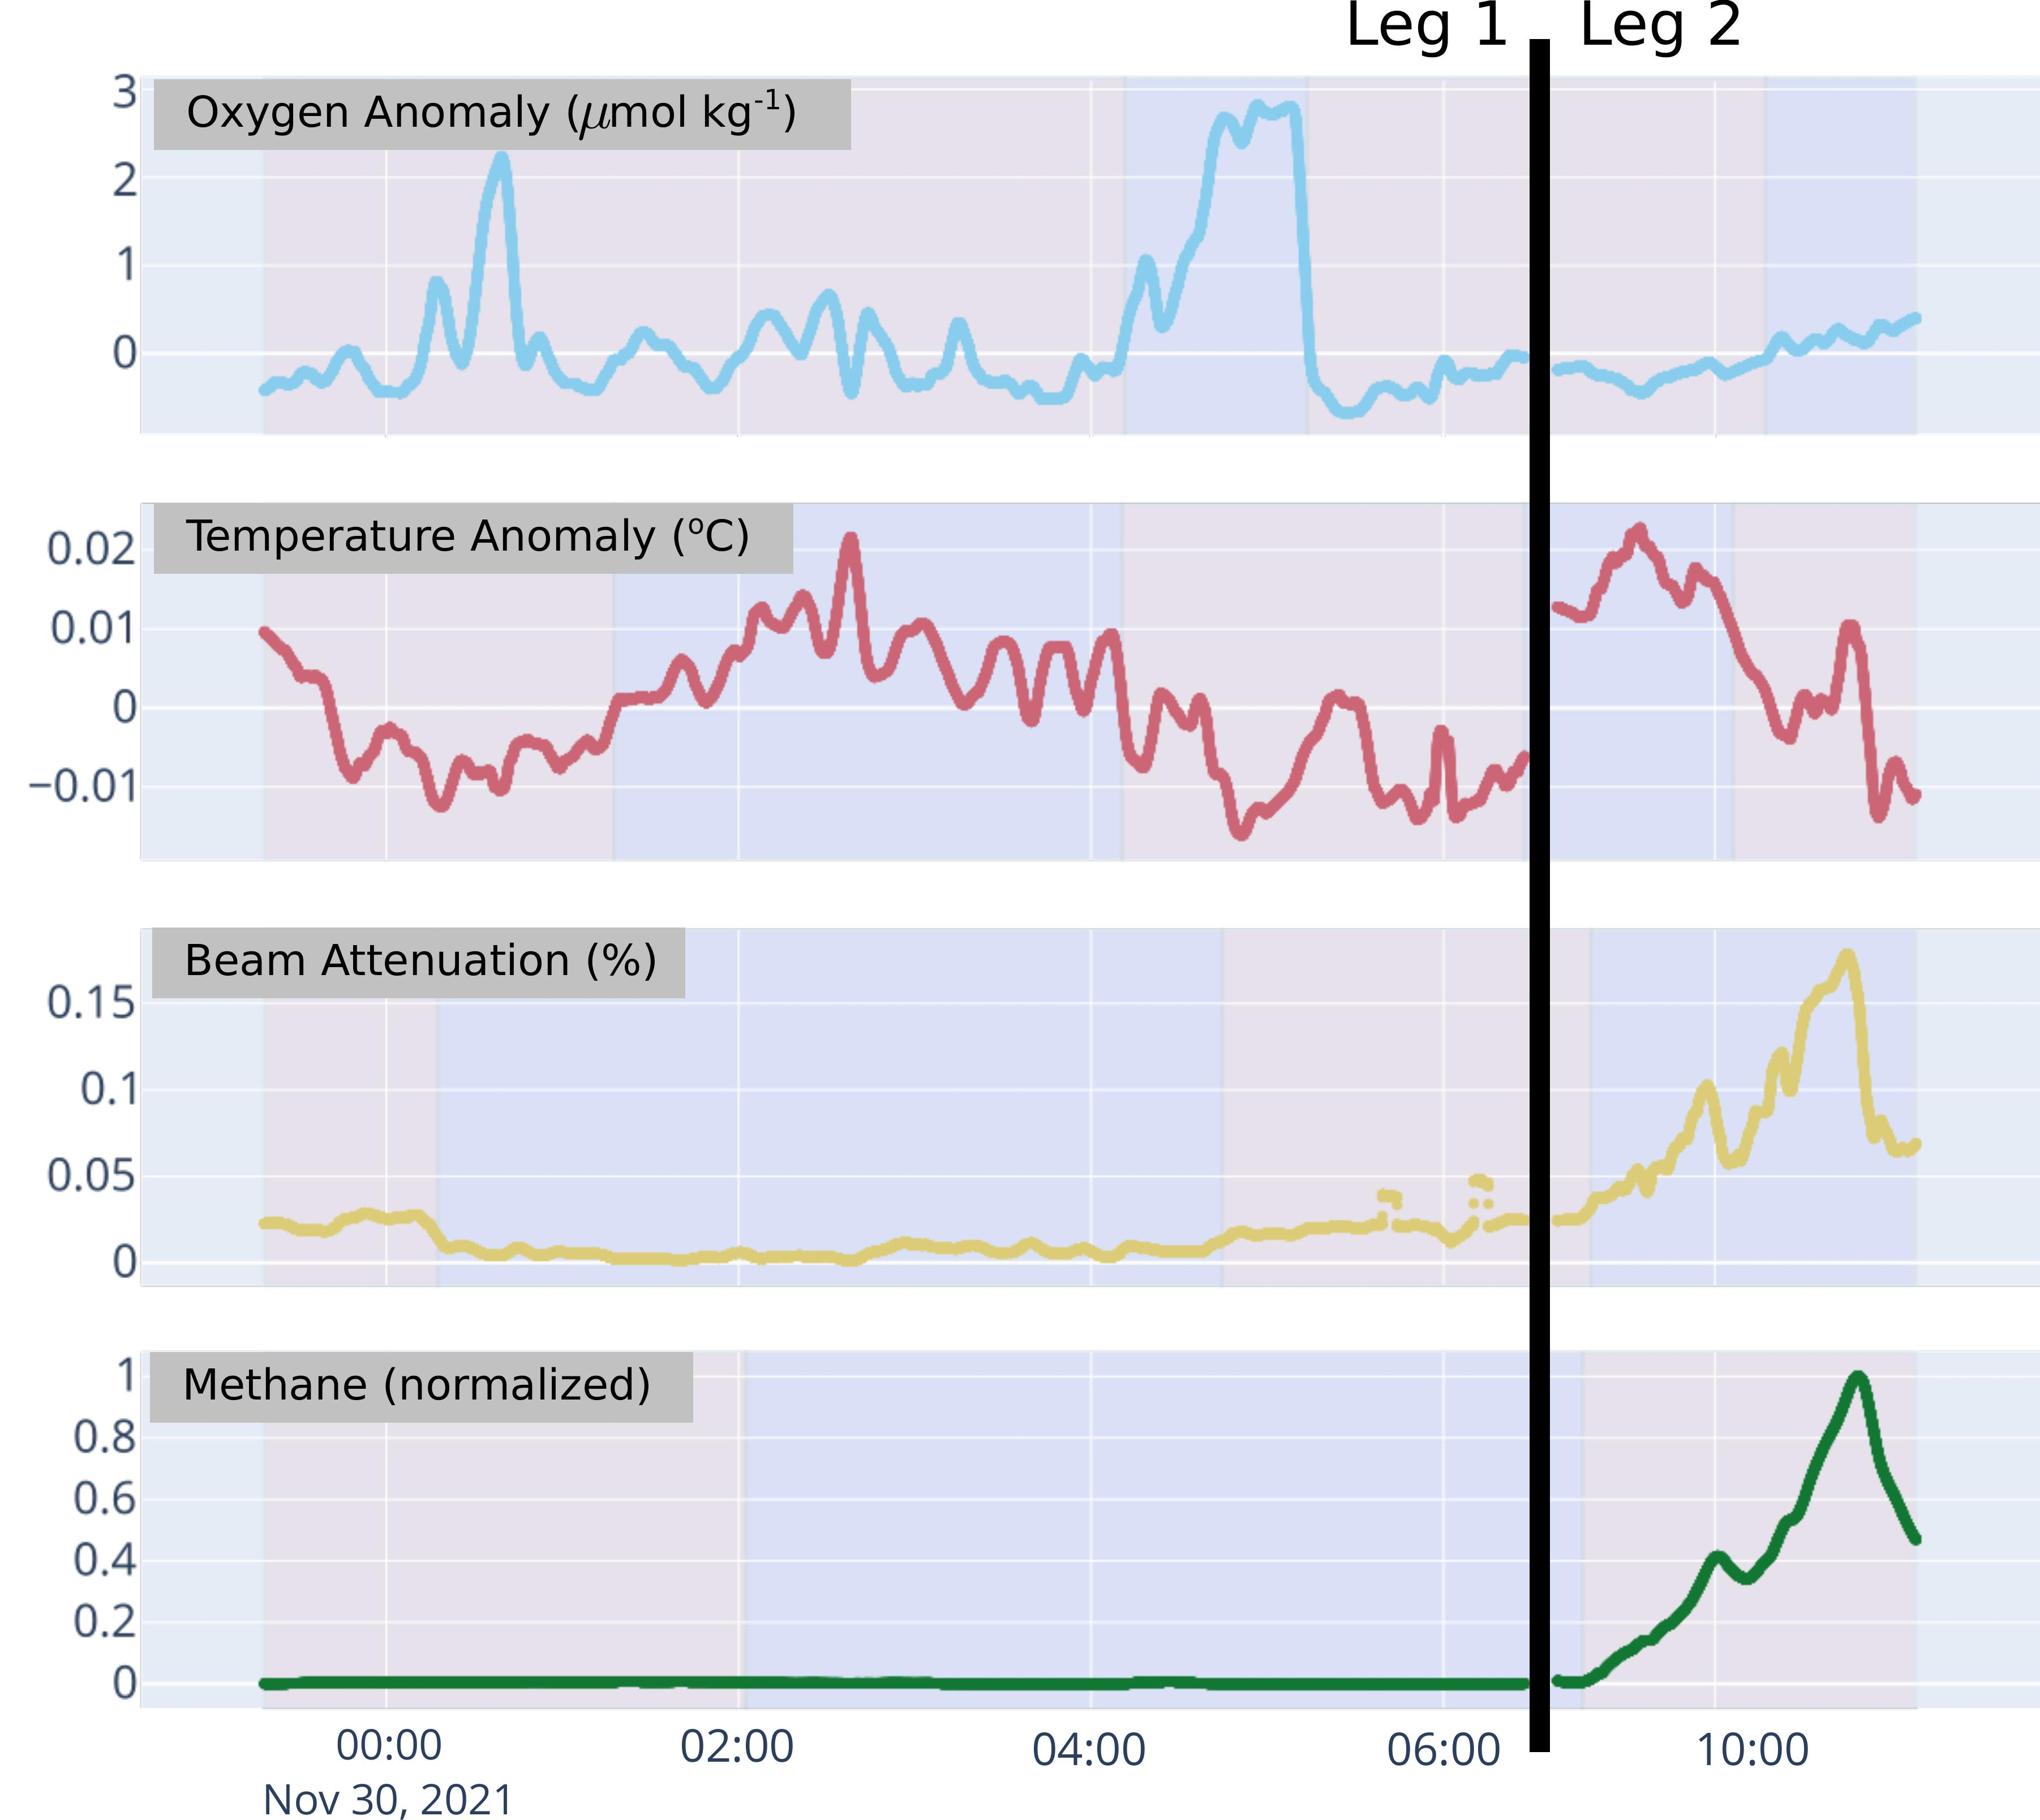
\includegraphics[width=1\columnwidth]{figures/chap3_rosette_regimes.jpg}
    \caption[Regime changes in rosette observations.]{\textbf{Regime changes in rosette observations.} Regimes, indicated as alternating blue and red regions, detected during the rosette transect with a 30 minute detection window.}
    \label{fig:rosette_regimes}
\end{figure}


With instruments mounted on \emph{Sentry}, in Fig.~\ref{fig:sentry_regimes}, clear ``steps'' of methane observed by Pythia each mark a regime in that data stream. Some of these steps are nearly coincident with regime changes in turbidity, temperature, and oxygen (particularly the steps at 06:30 and 09:30).  

\begin{figure}[h!]
    \centering
    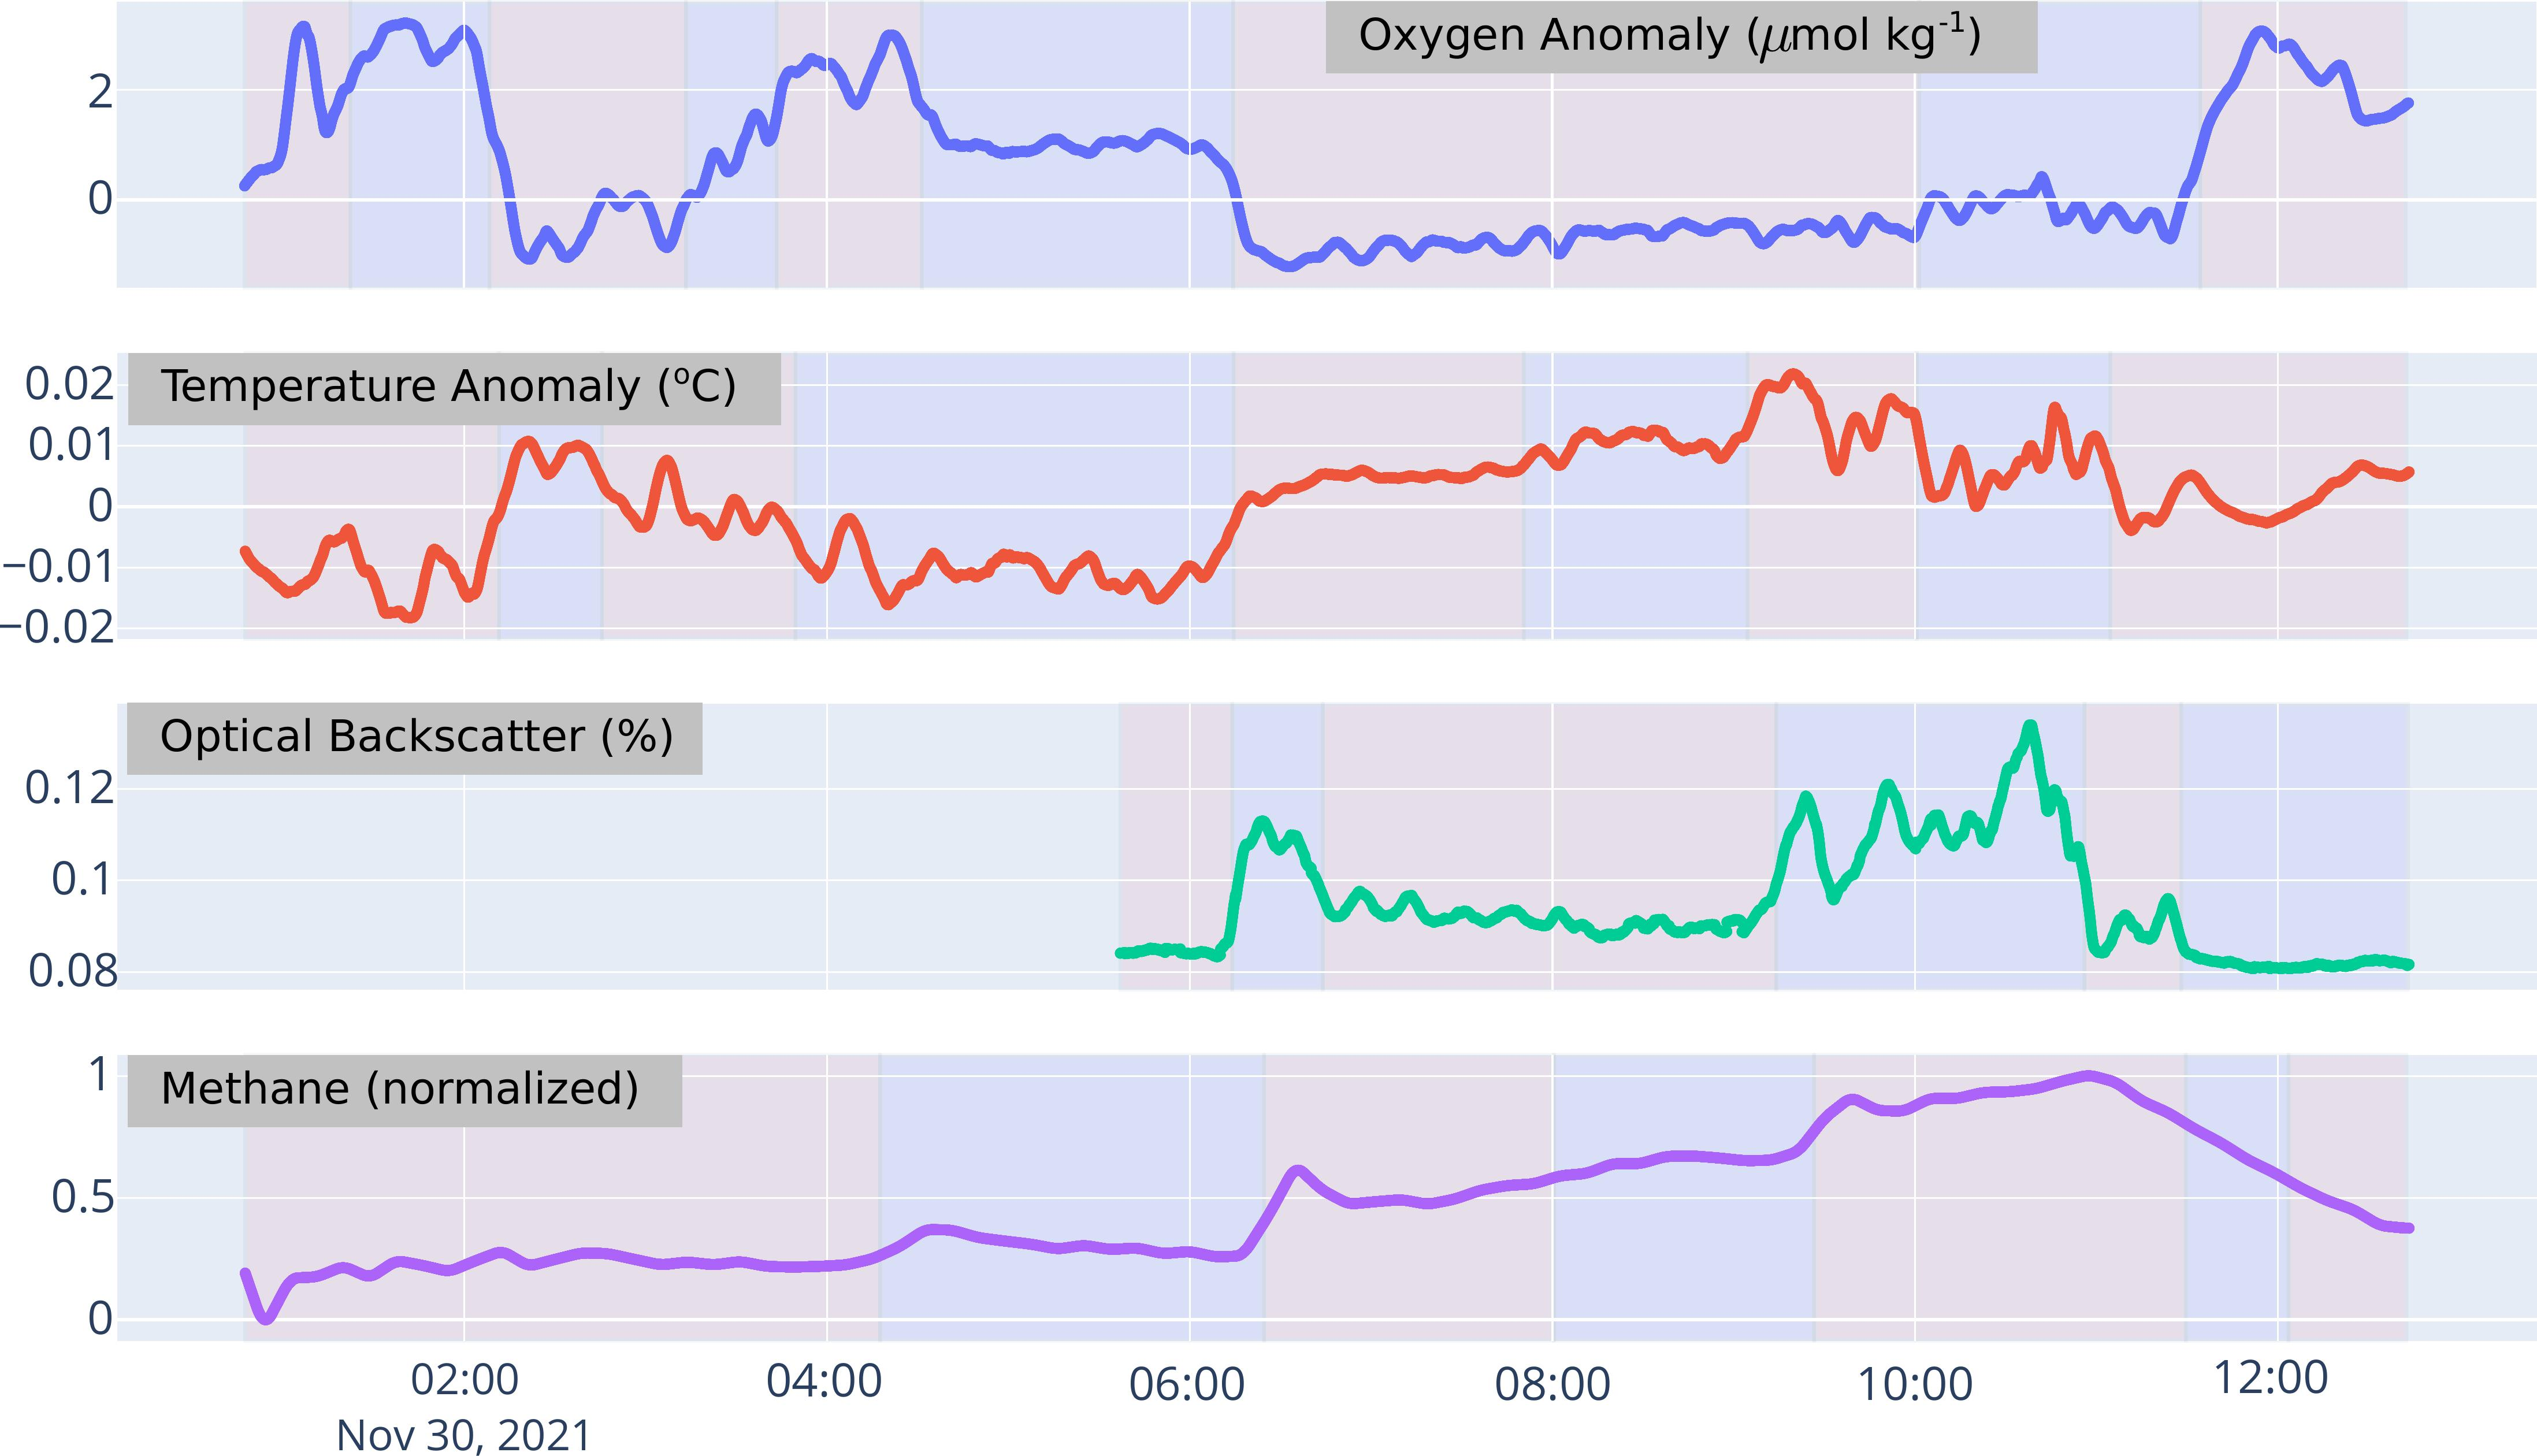
\includegraphics[width=1\columnwidth]{figures/chap3_sentry_regimes.jpg}
    \caption[Regime changes in AUV \Sentry observations.]{\textbf{Regime changes in AUV \Sentry observations.} Regimes, indicated as alternating blue and red regions, detected during the AUV \emph{Sentry} transect with a 30 minute detection window.}
    \label{fig:sentry_regimes}
\end{figure}

Regimes can be mathematically identified in streaming data, making this a potentially useful method to adopt for real-time hydrothermalism discovery. Coupled with absolute measurements by sensing instruments and rolling correlative structure, identifying water masses across multiple data streams can be done live from streaming data on the ship. The simplicity of the computation and the nature of these analysis techniques as data reduction methods (e.g., regimes can be reported as a single time stamp; cross-correlations over strategic sensor pairs could be reported as a single float) additionally make computing these measures onboard an AUV and reporting them back to watchstanders under data-limited transmission protocols (e.g., acoustic pings) feasible. 


\subsection{Methane in Deep Sea Exploration}
AUV and sensor deployments during expedition RR2107 served as an initial proving ground for the SAGE and Pythia \emph{in situ} methane instruments for deep sea exploration, and the utility of methane as a potential tracer for hydrothermalism discovery. During this transect both instruments observed significantly elevated methane over a span of several kilometers from a known hydrothermal source in Guaymas Basin. Methane proved to be a strong predictor for hydrothermalism that was not easily confounded by physical oceanographic events (e.g., mixing), giving it an advantage over oxygen, temperature, and salinity. Indeed, in this trial, each of the oxygen, temperature, and salinity instruments were impacted by an unknown physical feature not driven by hydrothermalism, but registered as similar scales of expected anomaly. Methane was also shown to be more expressive than ORP, which only registered a possible anomaly long after significant methane measurements were observed. Turbidity was a similarly useful and expressive feature of hydrothermalism in this basin, with similar detection scales to methane during this transect. Notably, for less strict detection criteria (i.e., thresholds) on detection, methane significantly outperformed turbidity in terms of detection scale (positive identification up to 6.8 km away, in contrast to 3.4 km for turbidity). Turbidity and methane together make for a strong pairing for hydrothermalism discovery. While neither one alone is a ``universal'' proxy for hydrothermal activity---not all hydrothermalism of interest produces particulate heavy smoke (i.e., diffuse flow fields) nor do all vents produce significantly elevated methane---they are complementary indicators which can assist in deep sea exploration for anomalous water masses derived from hydrothermalism. 

Collecting high resolution measurements of methane during this transect highlighted the rich structure of dissolved gasses in a neutrally buoyant plume layer over multiple kilometers, with multiple peak detections being possibly indicative of mixing novel and aging hydrothermal fluids, the contribution of multiple sources of hydrothermalism, or complicated internal mixing causing spatiotemporal multimodal distributions of dissolved gas ``pockets'' throughout the layer. Bottle samples collected on the research cruise verified the presence and general trend of methane observed by the instruments, but failed to resolve several features that may be of scientific interest. This motivates the use of \emph{in situ} methane sensors for future studies of hydrothermal fluids in the water column. 


\subsection{Enabling Better Decision-Making for Hydrothermalism Discovery}
Enabling the interpretation of real-time sensor data and adapting scientific missions accordingly are critical future skills for scientific expeditions and exploration in the deep sea. In preparation for this transect, a simple physical model was used to inform the design of the trajectory and monitored progress with live data displays for both the rosette and AUV \emph{Sentry}. While real-time data display for rosettes is now considered standard for oceanographic research, streaming capabilities of scientific data from autonomous platforms like \emph{Sentry} is a relatively new capability. This display infrastructure enabled the science team to make note of the OBS sensor error on \emph{Sentry} while performing the transect, caught a power and logging failure of the Pythia logger upon deployment (which, if left unresolved, would have meant an absence of all methane data associated with \emph{Sentry} for this analysis), and made real-time control and decision-making about the rosette positioning and bottle firing possible. While data presented here was analyzed after the mission, several of these analyses, including rolling correlation and regime detection, could be performed from streaming observations. As a whole, the techniques in this chapter present an opportunity for advancing technical infrastructure on a research vessel in order to enhance decision-making capabilities of the science party and engineering teams, both logistically to better diagnose instrument operation \emph{in situ} and scientifically to enhance data collection.

Real-time data collection and processing could have further implications for embodied intelligence as a tool for scientific expeditions. Using models, inference methods, and streaming data, autonomous agents like AUV \emph{Sentry} could be made capable of performing adaptive decision-making for sample collection. Hydrothermalism discovery has long been a motivating use case for intelligent autonomy at sea \autocite{yoerger2007autonomous, jakuba2007stochastic, branch2020demonstration, wang20203}. This transect experiment demonstrates the utility of simple models for tractable, intelligent planning, motivates the possibility of using methane as an additional, reliable data source for performing autonomous behaviors (e.g., adaptive sampling, tracking), and presents the opportunity to embed simple analytical methods for classifying hydrothermal fluids from sensor streams. Being able to both map the source of hydrothermal plumes with ROVs and chart the evolving nature of fluids in the mid-water with AUVs, would enable an advancement of scientific inquiries that could be pursued with respect to hydrothermalism in the deep ocean. Such queries include the detailed structure of multiple-source plume collision, directly measuring \emph{in situ} the 4D structure of mixing in neutrally buoyant plumes and buoyant plume stems, assessing biological activity supported by plume fluids, tracing the fate of dissolved gasses, and more. This work demonstrates that detection of hydrothermal sources is possible on the scale of several kilometers even from relatively small hydrothermal vents that are present in Guaymas Basin, and has taken initial steps to demonstrate core data infrastructure that can improve human decision-making in hydrothermalism discovery; future work and engagement will be focused on advancing these tools to enable the next generation of scientific inquiry in the deep ocean.
  % Frontiers Paper
  \chapter{Physically-Informed Uncertainty Models for Spatiotemporality}
\td{Need new intro for this section}


\section{Methodology}
\label{sec:methods}
Key to a physically informed model are the observations available and the model selection itself...\td{pithy introduction to the method here}


\subsection{Plume Detection: Treatment of Robotic Science Sensors}
\label{sec:sensor_models}
The observational data available from AUV \Sentry are continuous measurements from multiple science sensors. These data must first be processed into a data stream the can be used to train the \PHUMES model. In the hydrothermal charting task, there is no single sensor that can be used directly as a proxy for whether a parcel of fluid was hydrothermally derived \autocite{jakuba2007stochastic,preston2022discovering}. This lack of exact sensing is due to the variable values of temperature, chemistry, and particulate matter that persist within a plume structure. In the buoyant stem of a plume, positive temperature anomalies may be several degrees warmer compared to ambient seawater; however in the neutrally-buoyant plume layer, these anomalies may be on the scale of sensor noise (only a few hundredths of a degree). Chemistry anomalies may persist longer within a plume, but are subject to unknown and variable rates of microbial digestion or chemical reaction with the environment. Moreover, some chemical signatures may not specifically fingerprint hydrothermal anomalies, and could be equally indicative of other water-mass mixing events in the deep ocean. Finally, some oceanographic properties (e.g., temperature) vary in the water column as a function of depth, and so data must be detrended with respect to position in the water column. Taken together, the environmental complexity requires developing a sensing strategy that can fuse observations from multiple science sensors onboard \Sentry into a data product that indicates whether the robot encountered hydrothermal plume fluids. 

We elect to process the heterogeneous sensor stream into a binary measurement stream, drawing on the work in \autocite{jakuba2007stochastic}, to indicate whether \Sentry was in a plume or in background seawater\footnote{Access to a binary measurement for plume hunting has long been assumed in related work e.g.,  \autocite{tian2014behavior,saigol2009information}}. For this study, \td{back reference the previous chapter more here} we use a conductivity probe (salinity), temperature probe (temperature), oxidation-reduction potential (ORP) instrument (relative ``reactivity'' of water), optical backscatter (OBS) instrument (turbidity), optode (oxygen), and experimental spectroscopic instruments Pythia \autocite{michel2022gas,Harb:12} and SAGE \autocite{kapit2021dissolved,kapit2021measurement} (dissolved methane) to compute a binary measurement. Sensors are internally logged at variable rates, but interpolated and sub-sampled to a fixed 1 Hz frequency with a shared clock time for the purposes of directly comparing the instruments. Each of these sensors has its own physical characteristics and response to the chemistry of plume water. For example, ORP exhibits a large negative spike when first encountering plume water followed by a slow hysteresis back to a nominal values. Measurements of salinity, temperature, and oxygen are expected to be influenced not only by plume water, but background physical mixing in the ocean; turbidity, ORP, and methane are signals strongly associated with hydrothermalism because they are not persistent in background seawater. To account for the different ways in which sensors respond to plume waters, each sensor is processed individually to detect plume masses in each stream (see \cref{tab:sentry_instruments}). Weights are assigned to each sensor based on their individual reliability for identifying plume water, as determined by the science party and consulted experts in preparation for the research expedition. Observations are then classified as plume water or background water using corroboration across sensors: weighted detections for each sensor are summed together and we use a detection threshold to identify an observation as plume or background. A total corroboration score of 4 or more was used to classify an observation as plume. An example of this sensor applied to real \Sentry detections is shown in \cref{fig:detection_example}.

\begin{table}[h!]
    \centering
    \begin{tabular}{c|p{0.6\linewidth}|c}
        Quantity & Positive Plume Detection Criteria & Weight  \\
        \hline
        Salinity & Detrended practical salinity outside 3 standard deviations of the entire time series & 1 \\
        Temperature & Detrended temperatures above the 75th percentile of entire time series & 2 \\
        ORP & Detections less than -0.005 & 2 \\
        OBS & Optical attenuation above the 75th percentile of entire time series & 2 \\
        Oxygen & Detrended concentrations outside one-hour rolling computation of 3 standard deviations & 1 \\
        Methane & Normalized concentration above 0.3 & 2
    \end{tabular}
    \caption{\textbf{Instruments on AUV \Sentry and the criteria used to identify plume fluids for each instrument.} The weight is used to indicate relative trustworthiness of a plume detection for each sensor, and is used in a corroboration scheme that sums detections across sensors in order to make a final determination on whether an observation location contained a parcel of plume fluid or consisted of background seawater. Detrended data removes depth-related cross-sensitivity from the measurements; for example, temperature is stratified in the deep ocean, so to ignore the impacts of depth changes in the data stream, those effects are removed by ``detrending'' the data stream.}
    \label{tab:sentry_instruments}
\end{table}

\begin{figure} [h]
    \centering
    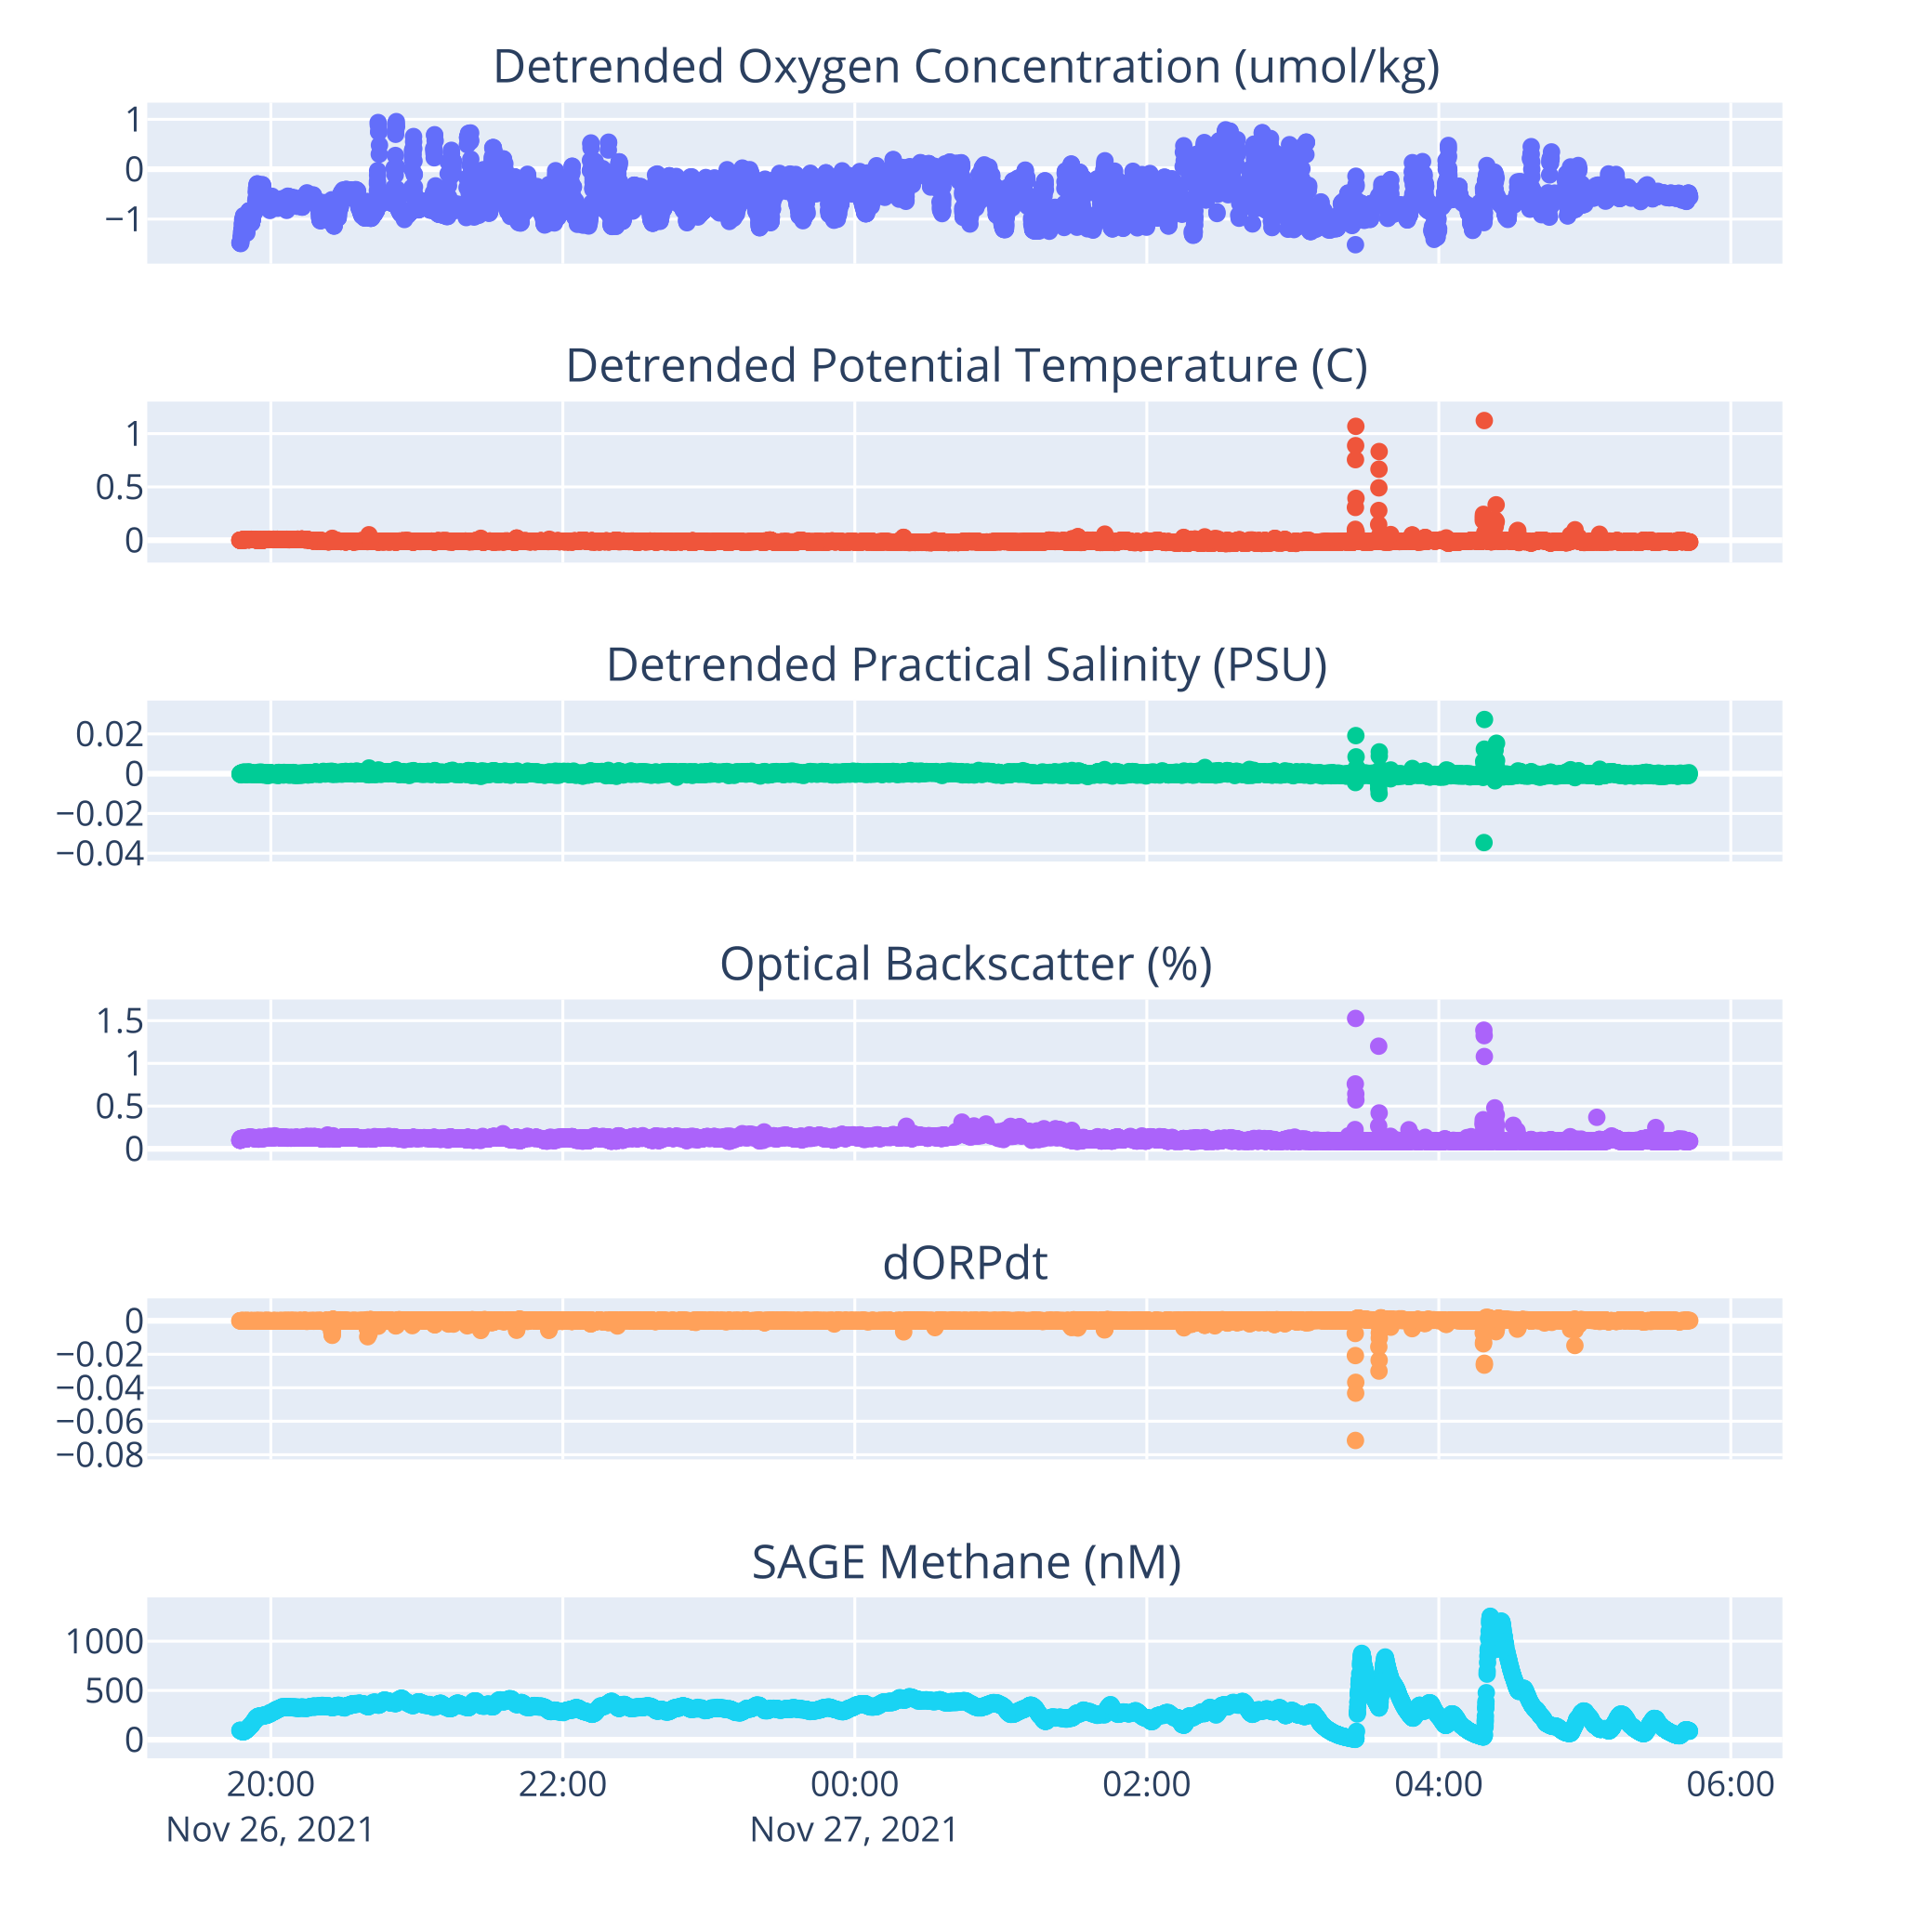
\includegraphics[width=0.45\columnwidth]{figures/binary_example_time.png}
    \hspace{.1in}
    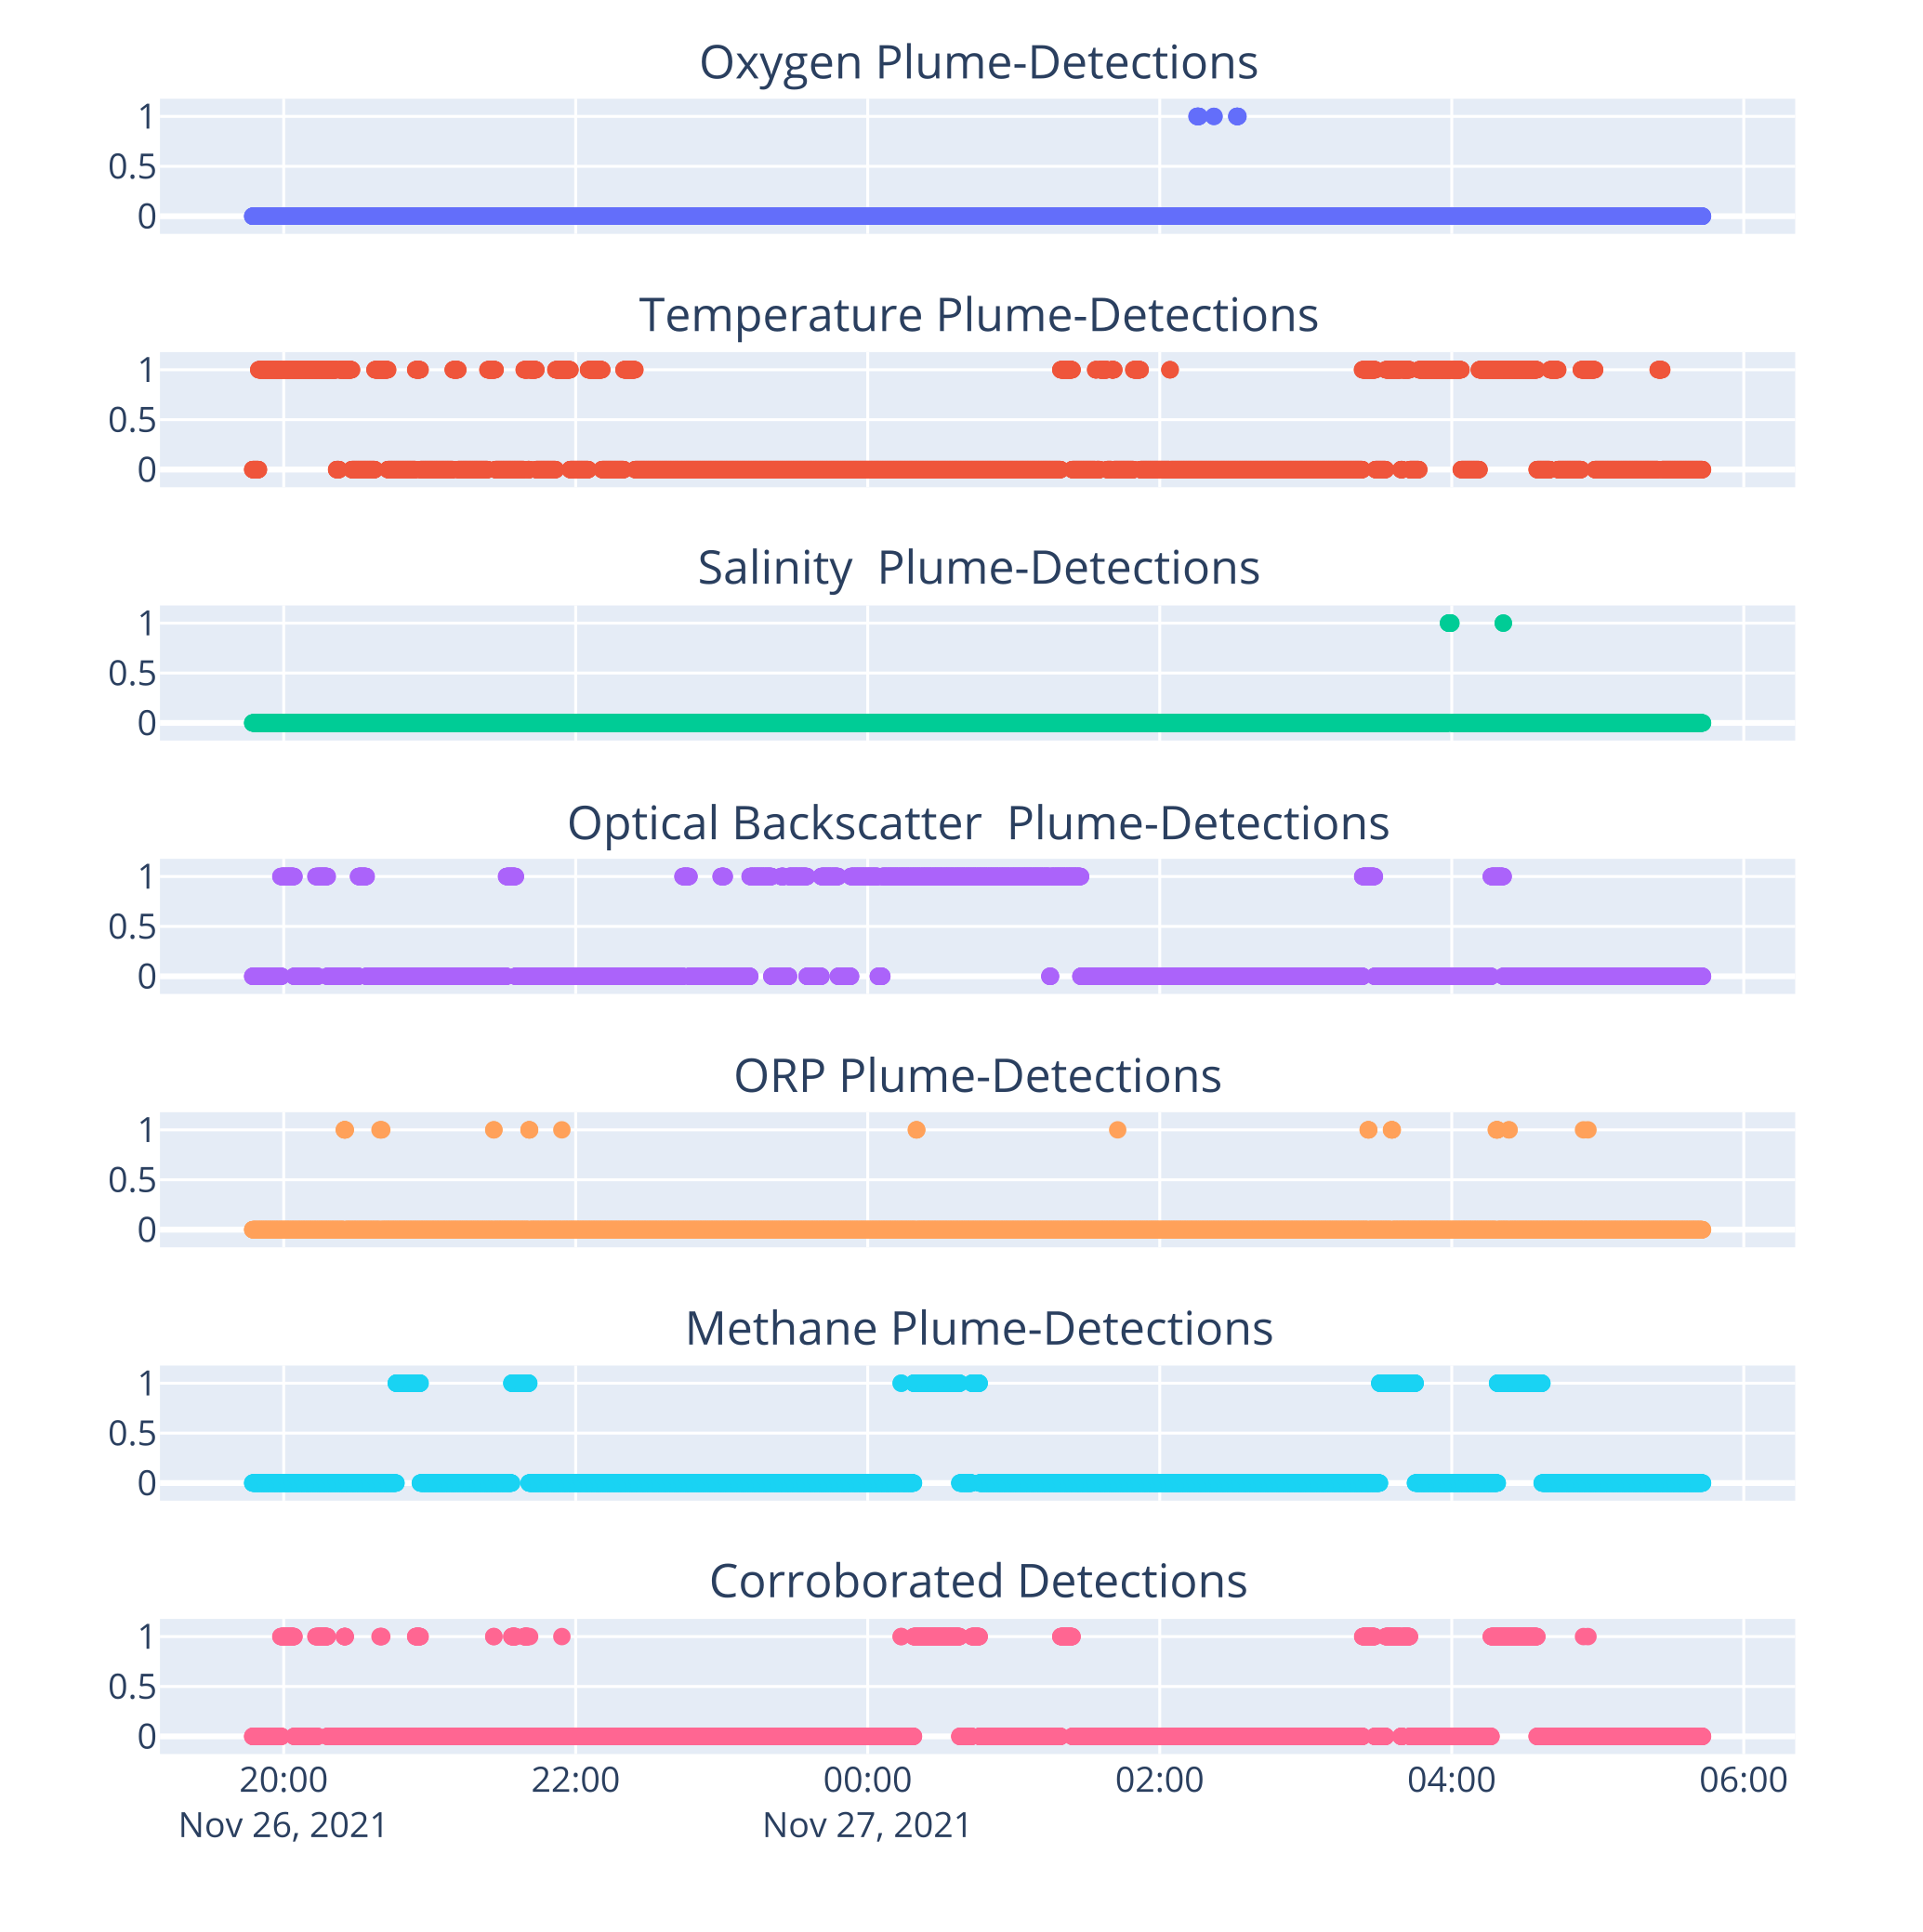
\includegraphics[width=0.45\columnwidth]{figures/binary_example_detections.png}
    \caption{\textbf{Example time series (left) and associated detections (right) over the AUV \Sentry sensor suite.} Oxygen, temperature, and salinity measurements are detrended using a linear transformation fit to depth vs. value plots. The time series demonstrates two types of plume detections. The first are ``obvious detections'' in which most sensors register strong anomalies (this happened twice toward the end of the deployment) and are most strongly associated with buoyant-stem derived fluids. The second are ``persistent-plume detections'' in which the robot traverses through water that is slightly more turbid, warm, or chemical-rich than background water over potentially long horizons (this happened early in the deployment and in the middle). Such detections are most strongly associated with neutrally-buoyant layers. The conservative corroboration detector successfully identifies both forms of plume water.}
    \label{fig:detection_example}
\end{figure}

% This approach for processing complex sensor observations into binary plume detections was initially developed by \autocite{jakuba2007stochastic}; our method is an adaptation of the process using recommendations in this previous work and in consultation with the science team we were directly collaborating with for this study. 
The result of our sensor model is to convert multiple, time-stamped sensor observations $s_{t, i} \in \R, \, i = 1, \dots, S$ to a time-stamped binary plume-detection $z_{p, t} \in \{0, 1\}$. These binary plume detections are then used to update our plume model and plan robot trajectories, as described in the following sections. The accuracy of this sensor model is currently uncharacterized, as there is no available ground truth in a field setting by which to verify the assigned classifications. Qualitatively, the classifications were reviewed by the science team and verified for their alignment with expert opinions on which label to assign.


%%%%%%%%%%%%%%%%%%%
% External Sensing 
%%%%%%%%%%%%%%%%%%
\subsection{External Sensing: Leveraging All Available Information}
\label{sec:external_current}
We deployed several sensing packages during the research cruise to collect relevant information about the state of temporally evolving crossflow $\x_c$ and ambient seawater properties. We leverage these external measurements within our \PHUMES instance in two ways. First, we characterize the background seawater stratification near a target site using a ship-board rosette\footnote{A rosette is often a metal frame on which oceanographic sensors and a carousel of water sampling containers are mounted. It is attached to a ship via a cable, and can be lowered and raised via a winch in vertical transects of the water column, or can be towed by a moving ship horizontally through the water column.} which takes vertical profiles of the water column. The empirical stratification function for Guaymas Basin is used within the physically-informed layer of \PHUMES and treated as a constant throughout the expedition. Second, we learn the crossflow transition function $T_c$. Critically there was no sensor on \Sentry during our expedition that could be used to measure the \emph{in situ} current magnitude and heading. While it may be possible to estimate $T_c$ solely from the binary observations of the plume, access to an external bottom-mounted tiltmeter on the seafloor during this expedition significantly relieved the burden of this inference process. These auxiliary sensors are introduced and discussed in detail in \cref{sec:field_description}. 

% For the former (1), measurements from a temperature and salinity sensor mounted to a ship-board rosette were used to define the depth-dependent density, temperature, and salinity stratification curves of the field site (Guaymas Basin) water column. The stratification curve is a function that describes the changes in density over depth in the ocean, and has implications for how a hydrothermal plume will interact with background seawater. 

% We learn $T_c$ (or, more precisely, the function $h$ by which $T_c$ is defined) by fitting a Gaussian process (GP) with composite radial-basis-function and periodic kernel functions to point observations of crossflow magnitude and heading observed by the tiltmeter. Approximately 3 days of observations were available for training. Crossflow parameters $\x_c$ in $\Ss$ were set with the expected mean of the trained GP. At present, a crossflow sensor is in development for \Sentry using existing acoustic technology onboard the robot; in such a configuration, estimating $T_c$ could be done simultaneously with the plume-charting task.

% PHUMES
\subsection{\PHUMES: Physically-informed Probabilistic Forecasts}
\label{sec:phumes}
\PHUMES is a modeling approach that can generate predictions of the distribution of a spatiotemporally evolving state from a history of sparse state-space observations. To quickly learn a predictive model of a spatiotemporal phenomenon, \PHUMES leverages access to analytical scientific simulators (when available) codified as systems of ordinary differential equations (ODEs). These simulators reduce the dimensionality of the inference problem from the full-state of the environmental phenomenon (e.g., a 4D volume in space and time with binary phenomenon measurement) to the dimensionality of the initial conditions and parameters of the simulator (which can then be used to populate the full-state for planning purposes). The use of ODE systems, as opposed to high-fidelity numerical simulators using partial differential equations (PDEs), is intentional; the computational requirement of most PDE systems used to model environmental phenomenon at the scales studied during expeditionary missions is intractable. In contrast, ODE systems are less well-resolved, but summarize the structure of an evolving phenomenon in a useful way for positioning a robot to encounter plume fluids and that can be enhanced by a generic probabilistic formulation wrapping the ODEs.

For hydrothermal plume charting, we use a time-averaged model of buoyant plume evolution through a weakly stratified fluid under crossflow as described in \autocite{tohidi2016highly} with modifications for seawater as adapted from \autocite{xu2012deep}, which for notational simplicity refer to as function $f(\cdot, \cdot)$. The crossflow ``bends'' the buoyant stem of the plume, and reduces the effective rise height of the plume by introducing more mixing. Using a modified cylindrical coordinate system in which $s$ represents a point along the axis described by the plume centerline and $\theta$ describes the vertical angle from the base of the plume, our \PHUMES simulator takes the form:

\begin{equation}
    \frac{dQ}{ds} = Q\sqrt{\frac{2(1+\lambda^2)}{M\lambda}}(\alpha|\frac{M}{Q} - U_a\cos\theta| + \beta|U_a\sin\theta|)
\end{equation}
\begin{equation}
    \frac{dM}{ds} - U_a\cos\theta\frac{dQ}{ds} = \frac{FQ}{M}\sin\theta 
\end{equation}
\begin{equation}
    U\sin\theta\frac{dQ}{ds} + M\frac{d\theta}{ds} = \frac{FQ}{M}\cos\theta
\end{equation}
\begin{equation}
    \frac{dF}{ds} = -QN^2\sin\theta
\end{equation}
\begin{equation}
    x_a = \int_0^s\cos\theta ds
\end{equation}
\begin{equation}
    h_a = \int_0^s \sin\theta ds
\end{equation}

where $U_a = U_a(z)$ is the ambient crossflow velocity, $Q = Q(s,\theta)$ represents the plume specific volume flux, $M = M(s, \theta)$ is the specific momentum flux, $F = F(s, \theta)$ is specific buoyancy flux, $N$ is the Brunt-V\"ais\"al\"a frequency, $\lambda$ is the ratio of the minor and major axis that define the plume cross-sectional ellipse, $x_a$ and $h_a$ represents the Cartesian transform of $s$ and $\theta$ within the plume's frame of reference, and $\alpha$ and $\beta$ are vertical and horizontal entrainment coefficients. To convert abstract notions of buoyancy and momentum flux to more readily interpretable and observable vent characteristics (e.g., vent area, fluid exit velocity), we can use the following relationships:

\begin{equation}
    Q_0 = \lambda u_0 \frac{A_0}{\pi}
\label{eq:heat_flux}
\end{equation}
\begin{equation}
    M_0 = Q_0 u_0
\label{eq:momentum_flux}
\end{equation}
\begin{equation}
    F_0 = g10^{-4}(T-T_0)Q_0
\label{eq:buoyancy_flux}
\end{equation}

\noindent where $A_0$ is the vent area, $u_0$ is the initial fluid velocity leaving the vent, $T$ is the temperature of fluid at the vent, and $T_0$ is the temperature of ambient seawater at the depth of the vent (note that temperature is the dominant component of density, $\rho$, for deep-sea hydrothermal plumes). Indeed, temperature, area, and exit velocity compose a sufficient set of parameters for representing the initial conditions of any particular plume and plume envelope calculation; these quantities, in addition to the mixing coefficients, form our set of $\x_p$ in $\Ss$ in the plume-charting POMDP. Correspondingly, $U_a$ and the global heading of the crossflow, $\Theta_a$ (not directly modeled in these equations, but can be trivially applied to $x_a$ and $x_h$ to convert plume-reference coordinates to global coordinates), form the parameters in $\x_c$ in $\Ss$.

With the simulator defined, we can now pose a specific inference problem: from observations of plume or background waters, what are the generating initial conditions (vent area, vent fluid temperature, vent fluid exit velocity) and seawater properties (horizontal mixing coefficient, vertical mixing coefficient, global current heading, and global current magnitude)? This allows us to place probability distributions over $\x_p$ and $\x_c$, over which we initially place an uninformative prior, $\Pi(\x_p)$ and $\Pi(\x_c)$ and aim to learn the posterior distributions $\Pi(\x_p | \Zz)$ and $\Pi(\x_c | \Zz)$ \footnote{We effectively separate inference over $\x_p$ and $\x_c$ given the observation model available; indeed we assume that observations of crossflow can be treated as independent of observations of plume detections. This is strongly supported in the practical deployment of \Sentry, when an external sensor was necessary to observe crossflow. If instead the sensors were co-located on \Sentry, inference over the joint posterior $\Pi(\x_p, \x_c | \Zz)$ could be done instead.}.

\begin{figure}[h!]
    \centering
    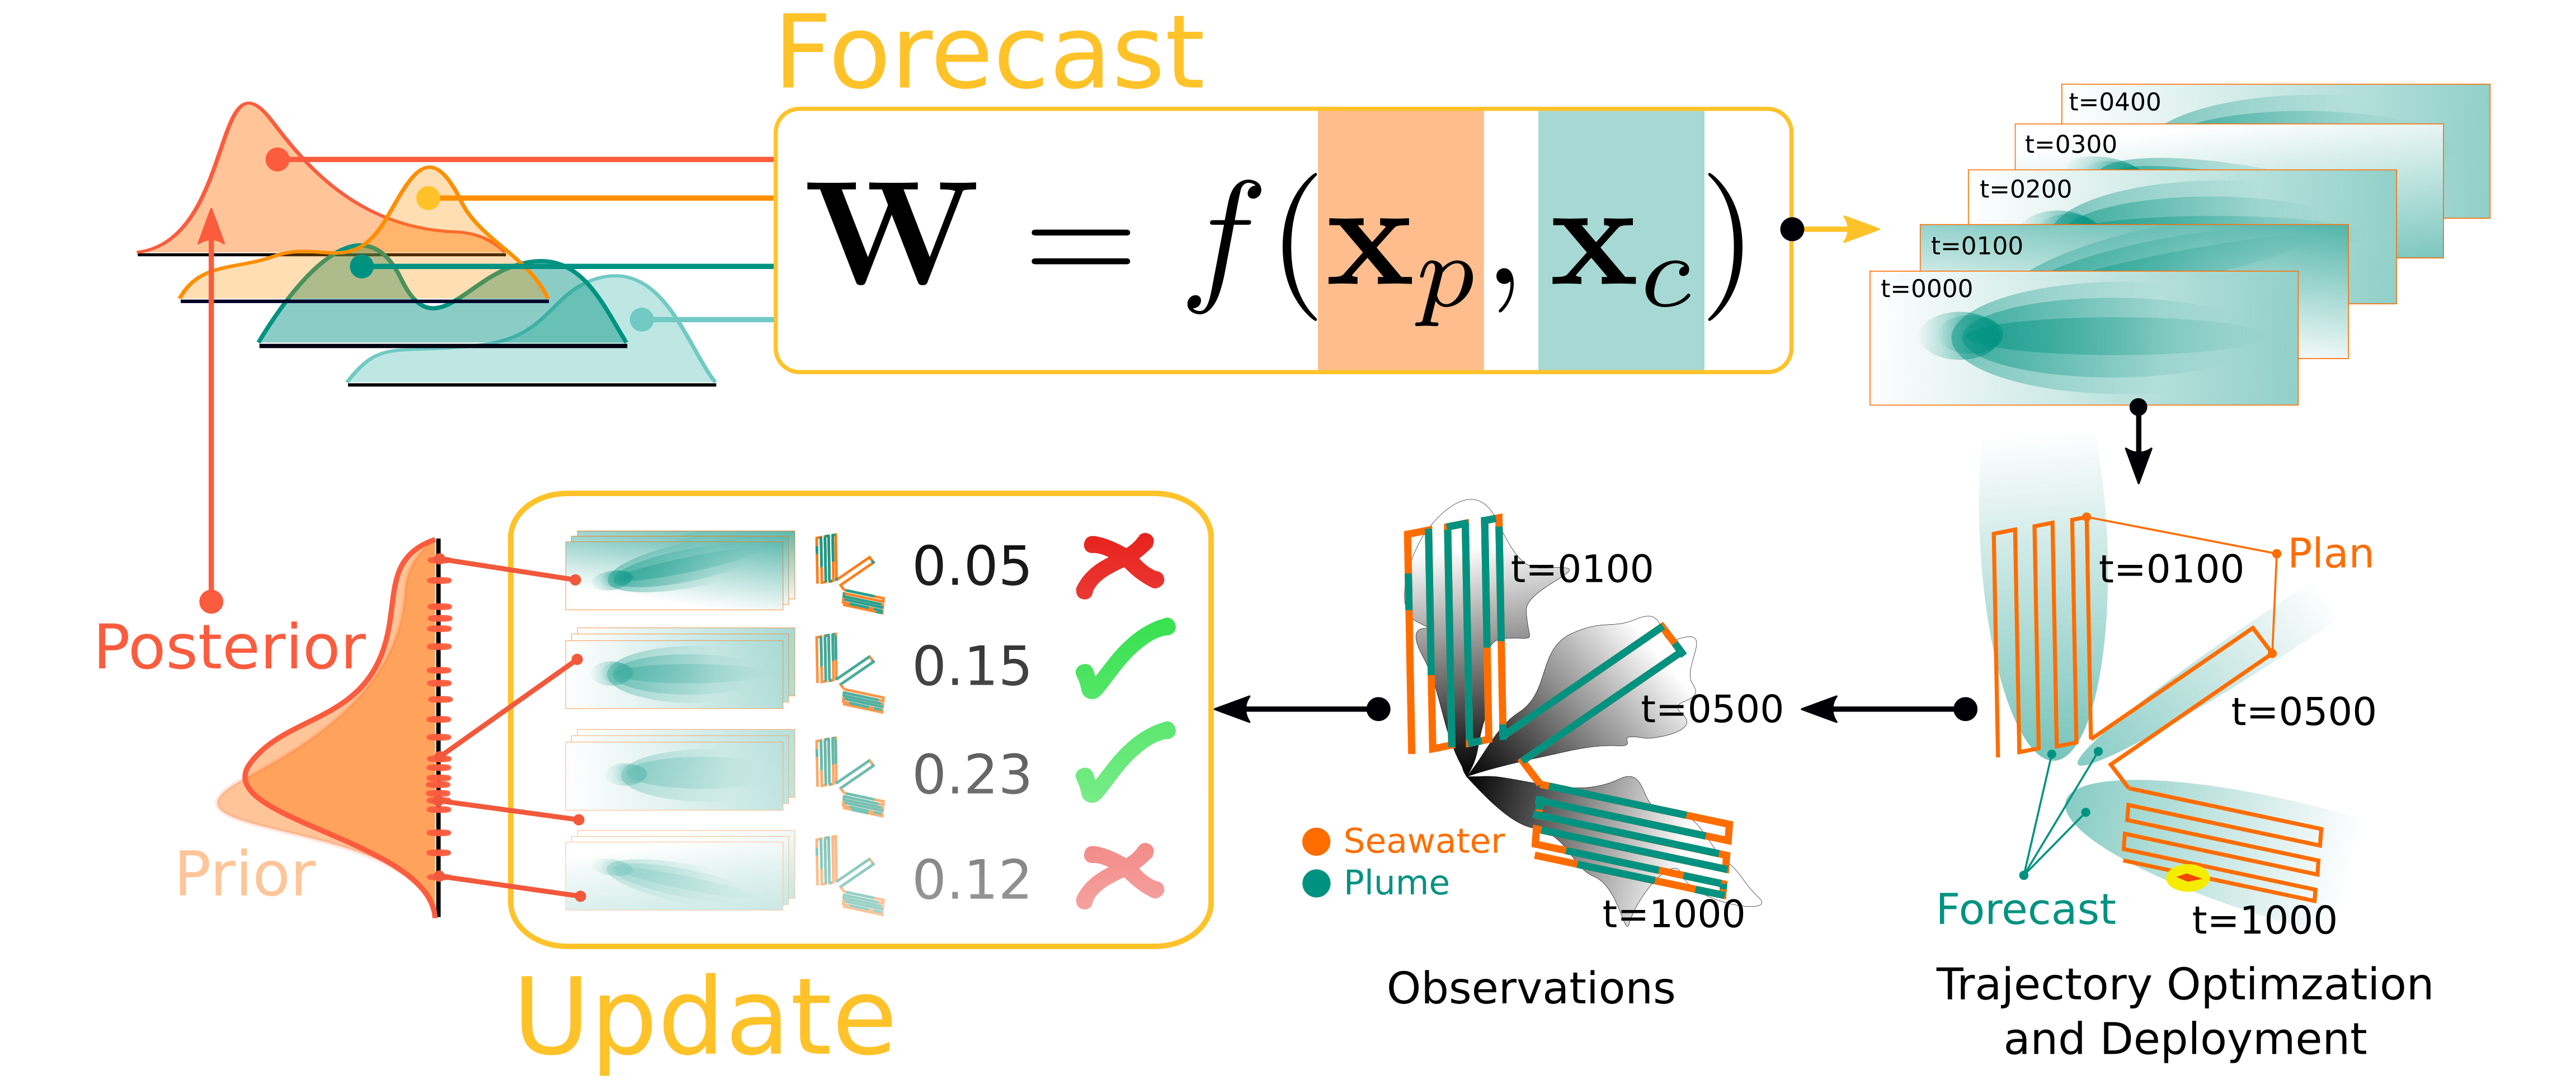
\includegraphics[width=1\columnwidth]{figures/phumes_diagram.png}
    \caption{\textbf{\PHUMES}: \phumes. \PHUMES is a model for forecasting the evolution of a spatiotemporal distribution trained on partial observations. \PHUMES generates forecasts by leveraging an embedded analytical model $f(\cdot, \cdot)$ that approximates the physics-driven evolution of a target distribution. This model is seeded with many samples from distributions placed over initial conditions, physical parameters, or temporal functions (such as $\x_p$ and $\x_c$ here). The composite result of this process is a forecast $\mathbf{W}$ that consists of a mean and variance of phenomenon occupancy in a 3D volume over snapshots of time. This forecast is provided to a trajectory optimizer which sets a deployment trajectory that is executed by a robot. The deployment generates a series of observations, which are then used to update the distributions of the generating distributions via MH-MCMC, which compares the gathered observations with the simulated observations of samples from the generating distributions. The resulting posterior update over the generating distributions is then used for the next planning iteration.}
    \label{fig:phumes}
\end{figure}

\PHUMES consists of two key phases: forecasting (forward simulation) and updating (inverse problem) (\cref{fig:phumes}). In the forecasting step, samples from the distributions of the initial conditions and seawater properties seed the simulator which is solved many times to create a set of plume-envelope samples in the full state space of the target phenomenon (and trajectory optimizer). Time is discretized over domain-specific key points, and any parameters reliant on time are sampled at those discrete points. The set of composite samples at each time is a ``forecast'' that is essentially a series of snapshots of the phenomenon. Precisely, \PHUMES generates a time-indexed $t \in \mathbb{T}$ composite estimate of the distribution of plume fluid in a 3D volume $\overbar{\mathbf{W}}$ by forward simulating time-dependent $M$ samples of the states $x_{p,t}^{(m)} \sim \Pi(\x_p(t))$ and $x_{c,t}^{(m)} \sim \Pi(\x_c(t))$ through the plume simulator $f(\cdot, \cdot)$:

\begin{equation}
    \overbar{\mathbf{W}}_t = \frac{1}{M}\sum_{m=1}^{M} f(x_{p,t}^{(m)}, x_{c,t}^{(m)}) \hspace{1cm} \forall t \in \mathbb{T}.
\end{equation}

The complete forecast $\overbar{\mathbf{W}}_t$ is then used by a trajectory optimizer to approximate the reward function $R([\x_p, \x_c, \x_r]^T, a) = \indic{\texttt{in\_plume}(\x_p, \x_c, \x_r, a)} \approx \indic{\texttt{in\_plume}(\overbar{\mathbf{W}}, a)}$. Equivalently, $\mathbf{W}$ is the robot's belief $b$, and as it consists of a set of samples, any statistical measure (the maximum \emph{a posteriori} estimator (MAP), maximum likelihood estimator (MLE), median, etc.) can be computed. For instance, the variance of the forecast $\mathbf{S}^2_W$ can be computed and used within an information-theoretic reward function (e.g., upper confidence bound), as contingent on the design of a downstream planner. 

After the trajectory optimizer yields a plan, \Sentry is deployed. For a single deployment, upwards of 20,000 observations may be available (each deployment is a minimum of 6 hrs in duration, up to 24 hrs, and sensor measurements are logged at 1 Hz). Using the filter described in \cref{sec:sensor_models}, AUV \Sentry provides observations of binary plume detections. Other sensors of opportunity described in \cref{sec:external_current} provide continuous crossflow magnitude and heading observations. These observations are collated into the sensor model $\Zz$.

At the update step of \PHUMES, the probability distributions over $\x_p$ and $\x_c$ are updated from observations $\Zz$. To find $\Pi(\x_c|\Zz)$ we use GP models for crossflow magnitude and heading as described in \cref{sec:external_current}. The GP kernel parameters are updated using a maximum-likelihood update following typical procedures \autocite{Rasmussen2004}. For $\Pi(\x_p | \Zz)$, we use a random-walk Metropolis-Hastings Markov Chain Monte Carlo (MH-MCMC) method \autocite{metropolis1953equation} to perform the update. Simulations of deployments are generated by solutions to the numerical model $f(\cdot, \cdot)$ seeded with samples from $\x_p$ and $\x_c$. The output of the simulations is directly compared via a likelihood model with the binary observations of plume waters collected by \Sentry. To handle binary measurements, we compute the Brier score \autocite{brier1950verification} over the set of real observations $\Zz$ and set of predictive probabilities $\rho(\cdot)$ of the corresponding simulated observations: $\frac{1}{|\Zz|}\sum_{i=1}^{|\Zz|} (\Zz^{(i)} - \rho(f(x_p, x_c)^{(i)}))^2$. In practice, the predictive probabilities $\rho(\cdot)$ are set according to a false positive rate (the observation is a 1, and the simulation is a 0) and false negative rate (the observation is a 0, and the simulation is a 1) established in consultation with instrument experts on the science team; they are set to 0.1 and 0.3, respectively. With the likelihood model applied, an acceptance criteria of the likelihood and evaluated priors over samples of $\x_p$ is defined, and samples probabilistically accepted or rejected accordingly. As MH-MCMC inference method is a chaining procedure, each sample of $\x_p$ selected is informed by the last, and the cumulative distribution of all accepted samples is guaranteed to converge to the true underlying distribution for each of the elements in $\x_p$ for long enough chains. The posterior distribution $\Pi(\x_p | Z)$ is set as the new sampling distribution for the next forecast to be generated.

\subsection{Available Oceanographic Instrumentation}
\label{sec:ops_sensors}
Observations from external sensors, summarized in \cref{tab:ext_sensors} and visualized in \cref{fig:ext_sensors}, were incorporated into the initial conditions, temporal functions, and seawater properties that define the analytical model in \PHUMES as described in \cref{sec:external_current}. Vent characteristics (i.e., vent area, vent fluid velocity, fluid temperature at the vent) were measured by ROV \emph{JASON} during other field operations in the expedition. \emph{JASON} carried a camera system and temperature wand. Measuring temperature with an ROV is precise, and so we directly use the observation of temperature by \emph{JASON}, \SI{340}{\celsius}, as the initial condition for vent fluid temperature in the \PHUMES model trained with at-sea data. Vent area and vent fluid velocity are measured with cameras onboard ROV \emph{JASON}. Using a \SI{10}{\centi\meter} spaced set of laser points that \emph{JASON} can toggle on and off \emph{in situ}, the vent area is extrapolated from an estimate of vent diameter from pixel-to-distance conversion in still images. Using this method, an area of approximately \SI{1.7}{\meter\square} was estimated, and used to center a uniform distribution over vent area to be updated with \PHUMES. Vent exit velocity was estimated by applying particle imaging velocimetry (PIV) \autocite{zhang2019time} to 4K video of the turbid fluids at the vent. PIV methods track turbulent parcels that have high cross-correlation values between frames of a video. By tracking many parcels over several frames, PIV yields a vector field of velocity estimates that can be averaged to establish a mean estimate for a region. Using \verb|PIVLab|, an open-source \verb|MATLAB| library \autocite{thielicke2021particle,thielicke2014pivlab,thielicke2014flapping}, we estimated a fluid exit velocity of \SI{0.7}{\meter\per\second}, and similarly use this as the center of a uniform prior placed on exit velocity for \PHUMES to update.

\begin{table}[h!]
    \centering
    \begin{tabular}{c|c|c|c}
        Platform & Instrument & Data Product & \PHUMES Incorporation \\
        \hline
        ROV \emph{JASON} & Camera & Vent Area &Informs prior over vent area \\
        ROV \emph{JASON} & Camera & Fluid Exit Velocity & Informs prior over fluid exit velocity \\
        ROV \emph{JASON} & Temperature wand & Vent Temperature  & Sets temperature initial condition \\
        Rosette & CTD probe & Water Column Stratification & References for analytical model \\
        Tiltmeter & Accelerometer & Current magnitude, heading & Use trained GP in forecast sampling \\
    \end{tabular}
    \caption{\textbf{Summary of auxiliary data.} External equipment and opportunistic data available from other operations during the field expedition that was used to inform the \PHUMES model within \PHORTEX used for at-sea trials.}
    \label{tab:ext_sensors}
\end{table}

In addition to \emph{JASON}, vertical profiles from a rosette of ambient seawater background salinity and temperature were available. As reference density and density stratification for a body of water are parameters of the analytical model (in order to compute buoyancy flux for the hydrothermal fluid), these profiles were used directly for this purpose. As the data had small amounts of noise, we fit simple Gaussian Process (GP) models with radial-basis function (RBF) kernels to each of temperature and salinity from a conductivity-temperature-depth (CTD) probe on the platform using \verb|GPytorch| (100 iterations, learning rate 0.1), and use the trained mean function within \PHUMES.

Finally, a tiltmeter (an instrument that is fixed to the seafloor on one end, and is allowed to tilt under the effects of crossflow) was available and deployed on the seafloor for three days during the cruise. Data collected from this instrument can be used to compute crossflow magnitude and heading. We observed a maximum crossflow magnitude of approximately \SI{0.1}{\meter\per\second}, and both magnitude and heading appeared to be semi-cyclic, following a pattern established by tidal charts produced by Centro de Investigaci\'on Cient\'ifica y de Educaci\'on Superior de Ensenada (CISESE) for the time period of the expedition\footnote{Charts available from: \url{www.predmar.cicese.mx/calendarios}}. Time-varying currents of magnitudes between 0.1-\SI{0.5}{\meter\per\second} sweeping from the northwest to southwest were previously reported in \autocite{scholz2019shelf}, corroborating our observations. We similarly trained a GP with RBF kernel for each of current magnitude and heading using \verb|GPytorch| (magnitude model: 100 training iterations, learning rate 0.5; heading model: 200 training iterations, learning rate 0.1), and used the trained GP within the sampling framework for \PHUMES to generate forecasts. 

\begin{figure}[h!]
    \centering
    \includegraphics[width=1\columnwidth]{figures/external_sensors.png}
    \caption{\textbf{Auxiliary data products used in \PHUMES.} External equipment (ROV \emph{JASON}, tiltmeter, and rosette) provided opportunistic data products during the field expedition that were incorporated into \PHUMES. The ROV \emph{JASON} was used to determine prior estimates for the plume source parameters. The rosette collected vertical temperature and salinity profiles which are used to compute stratification in the basin. A GP is trained over the data, and the mean is visualized in the lower right panel. The tiltmeter records data of current magnitude and heading; a GP was trained over both functions and is visualized in the lower left panel. Heading is reported in compass-rose orientation.}
    \label{fig:ext_sensors}
\end{figure}

\section{Experimental Results: Simulation and Field Trials}
\label{sec:experiments}

% Environment
\subsection{Simulation Experiments}
We investigate the performance of \PHORTEX in a simulated environment designed to replicate the field deployment closely. In the simulation, a point robot is tasked with collecting spatially and temporal diverse samples of an advecting plume. Each simulation is a three-dive series in which \PHORTEX starts with an uninformative prior over $\x_p$ and executes an initial naive survey (as would occur in a realistic field scenario), then iteratively updates \PHORTEX with collected observations and uses the the trajectory optimizer discussed in \cref{sec:to} to perform two more dives. We perform 10 three-dive simulations for each sampling/planning altitude of \SI{100}{\meter} and \SI{150}{\meter} in the same environment. Each single dive in the three-dive sequence is designed to be 12 hrs of simulated time, on a scale similar to the field deployment missions. 

In the simulator, the underlying analytical model in \PHUMES is used to generate a ground-truth environment that closely matches the conditions of the real-world vent using available data. The simulated environment has vent conditions of \SI{300}{\celsius}, 34.608 PSU salinity, \SI{0.8}{\meter\squared} orifice area, and \SI{0.6}{\meter\per\second} initial fluid velocity. The simulated environment sets the mixing coefficients to 0.15 and 0.2 for horizontal and vertical mixing, respectively. The current function sweeps a generated plume from due North to due East over the course of 12 hours of simulation time, and the magnitude cyclically varies with a beginning and end point of \SI{0.11}{\meter\per\second} and minimum at \SI{0.04}{\meter\per\second}. The generating current functions and snapshots of the true environment are provided in \cref{fig:sim_env}.

\begin{figure}[h!]
    \centering
    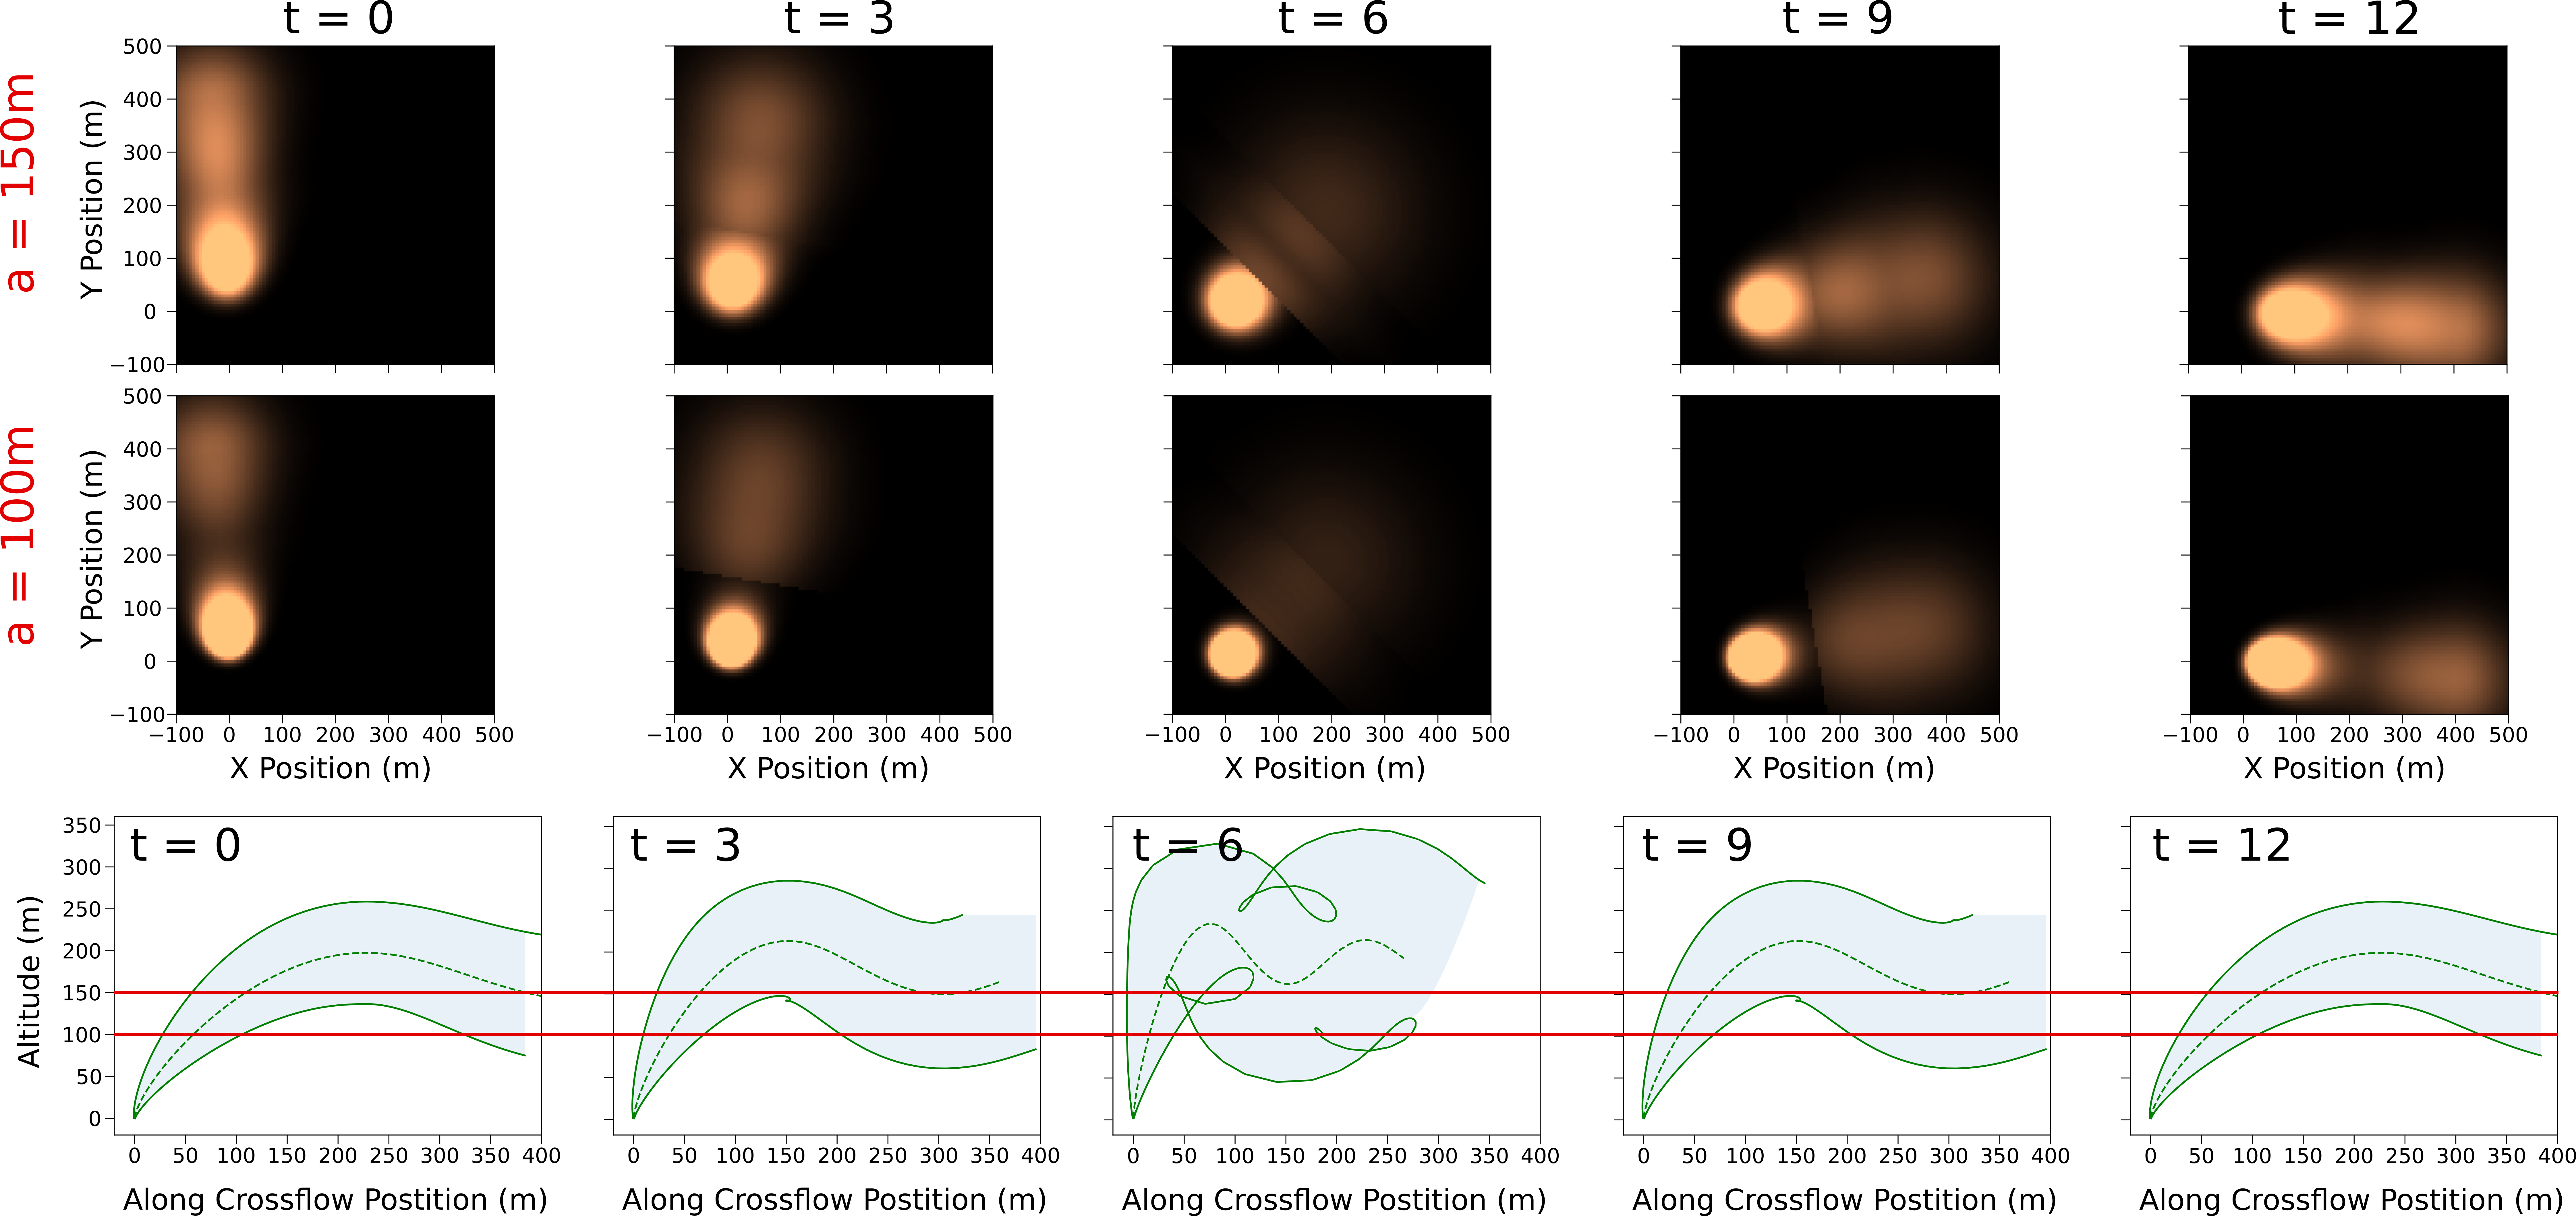
\includegraphics[width=1\columnwidth]{figures/sim_env.png}
    \caption{\textbf{Simulated field trial environment.} Generated environment for simulation trials at different snapshots for altitudes of \SI{100}{\meter} and \SI{150}{\meter}. As the current magnitude and heading changes, the plume expression changes shape and location over 12 hours. Plume intensity is shown in orange in the top plots. The bottom plots show a vertical cross-section of the plume envelope, along the crossflow direction, at different points in the tidal cycle, with the \SI{100}{\meter} and \SI{150}{\meter} horizontal planes marked.}
    \label{fig:sim_env}
\end{figure}

In these experiments, the \PHUMES model must estimate the vent area, vent fluid velocity, and both mixing coefficients from plume observation in the water column, starting with uninformative priors over each of these targets. A noisy current magnitude and heading function is provided to \PHUMES for use in the forecasting and updating step, as would typically be available from, for example, an auxiliary tiltmeter sensor (\cref{sec:aux_sensors}). For the \PHUMES update, 150 samples from an MH-MCMC chain are used to approximate the posterior distributions over the inference targets (this excludes an initial 50 samples of burn-in). In the first simulated dive, the robot executes a base-case uniformed lawnmower trajectory, placed to intersect the sweeping movement of the current. This trajectory is \SI{15}{\meter} in resolution, and covers a \SI{500}{\meter} by \SI{500}{\meter} area, with no rotation. For the second and third dives, trajectories are optimized using \PHORTEX for the 12-hour mission and consist of four, 3-hour long chained lawnmowers. Each lawnmower in the chain has a fixed resolution of \SI{10}{\meter}, and the height, width, origin, and orientation of each lawnmower are optimized to collect the most reward based on a plume forecast using the maximum \emph{a posteriori} (MAP) sample returned by the \PHUMES model for the four inference targets. The robot travels at approximately \SI{0.5}{\meter\per\second}, collecting binary observations every meter that is traveled. 

% Quality for this task is defined as collecting a high-proportion of in-plume samples over the course of a dive, revisiting a plume over the course of a dive, and collecting in-plume samples as far from the vent as the robot drives. 
\subsection{Simulation Experiments: Results}
\cref{fig:sim_traj_example} shows example planned trajectories and \cref{fig:sim_traj_perform} shows the distribution of each of the metrics of interest presented in \cref{sec:eval_metrics}---proportion in plume, spatial utilization, temporal utilization---for the three dives at each altitude tested in the trials. These results demonstrate that the \PHORTEX optimized trajectories significantly outperform the naive baseline, collecting over twice the proportion of samples in-plume, at least doubling the number of hours that the robot spends in a plume, and improving spatial utilization to nearly 100\% from 60-70\%. 

\begin{figure}[h!]
    \centering
    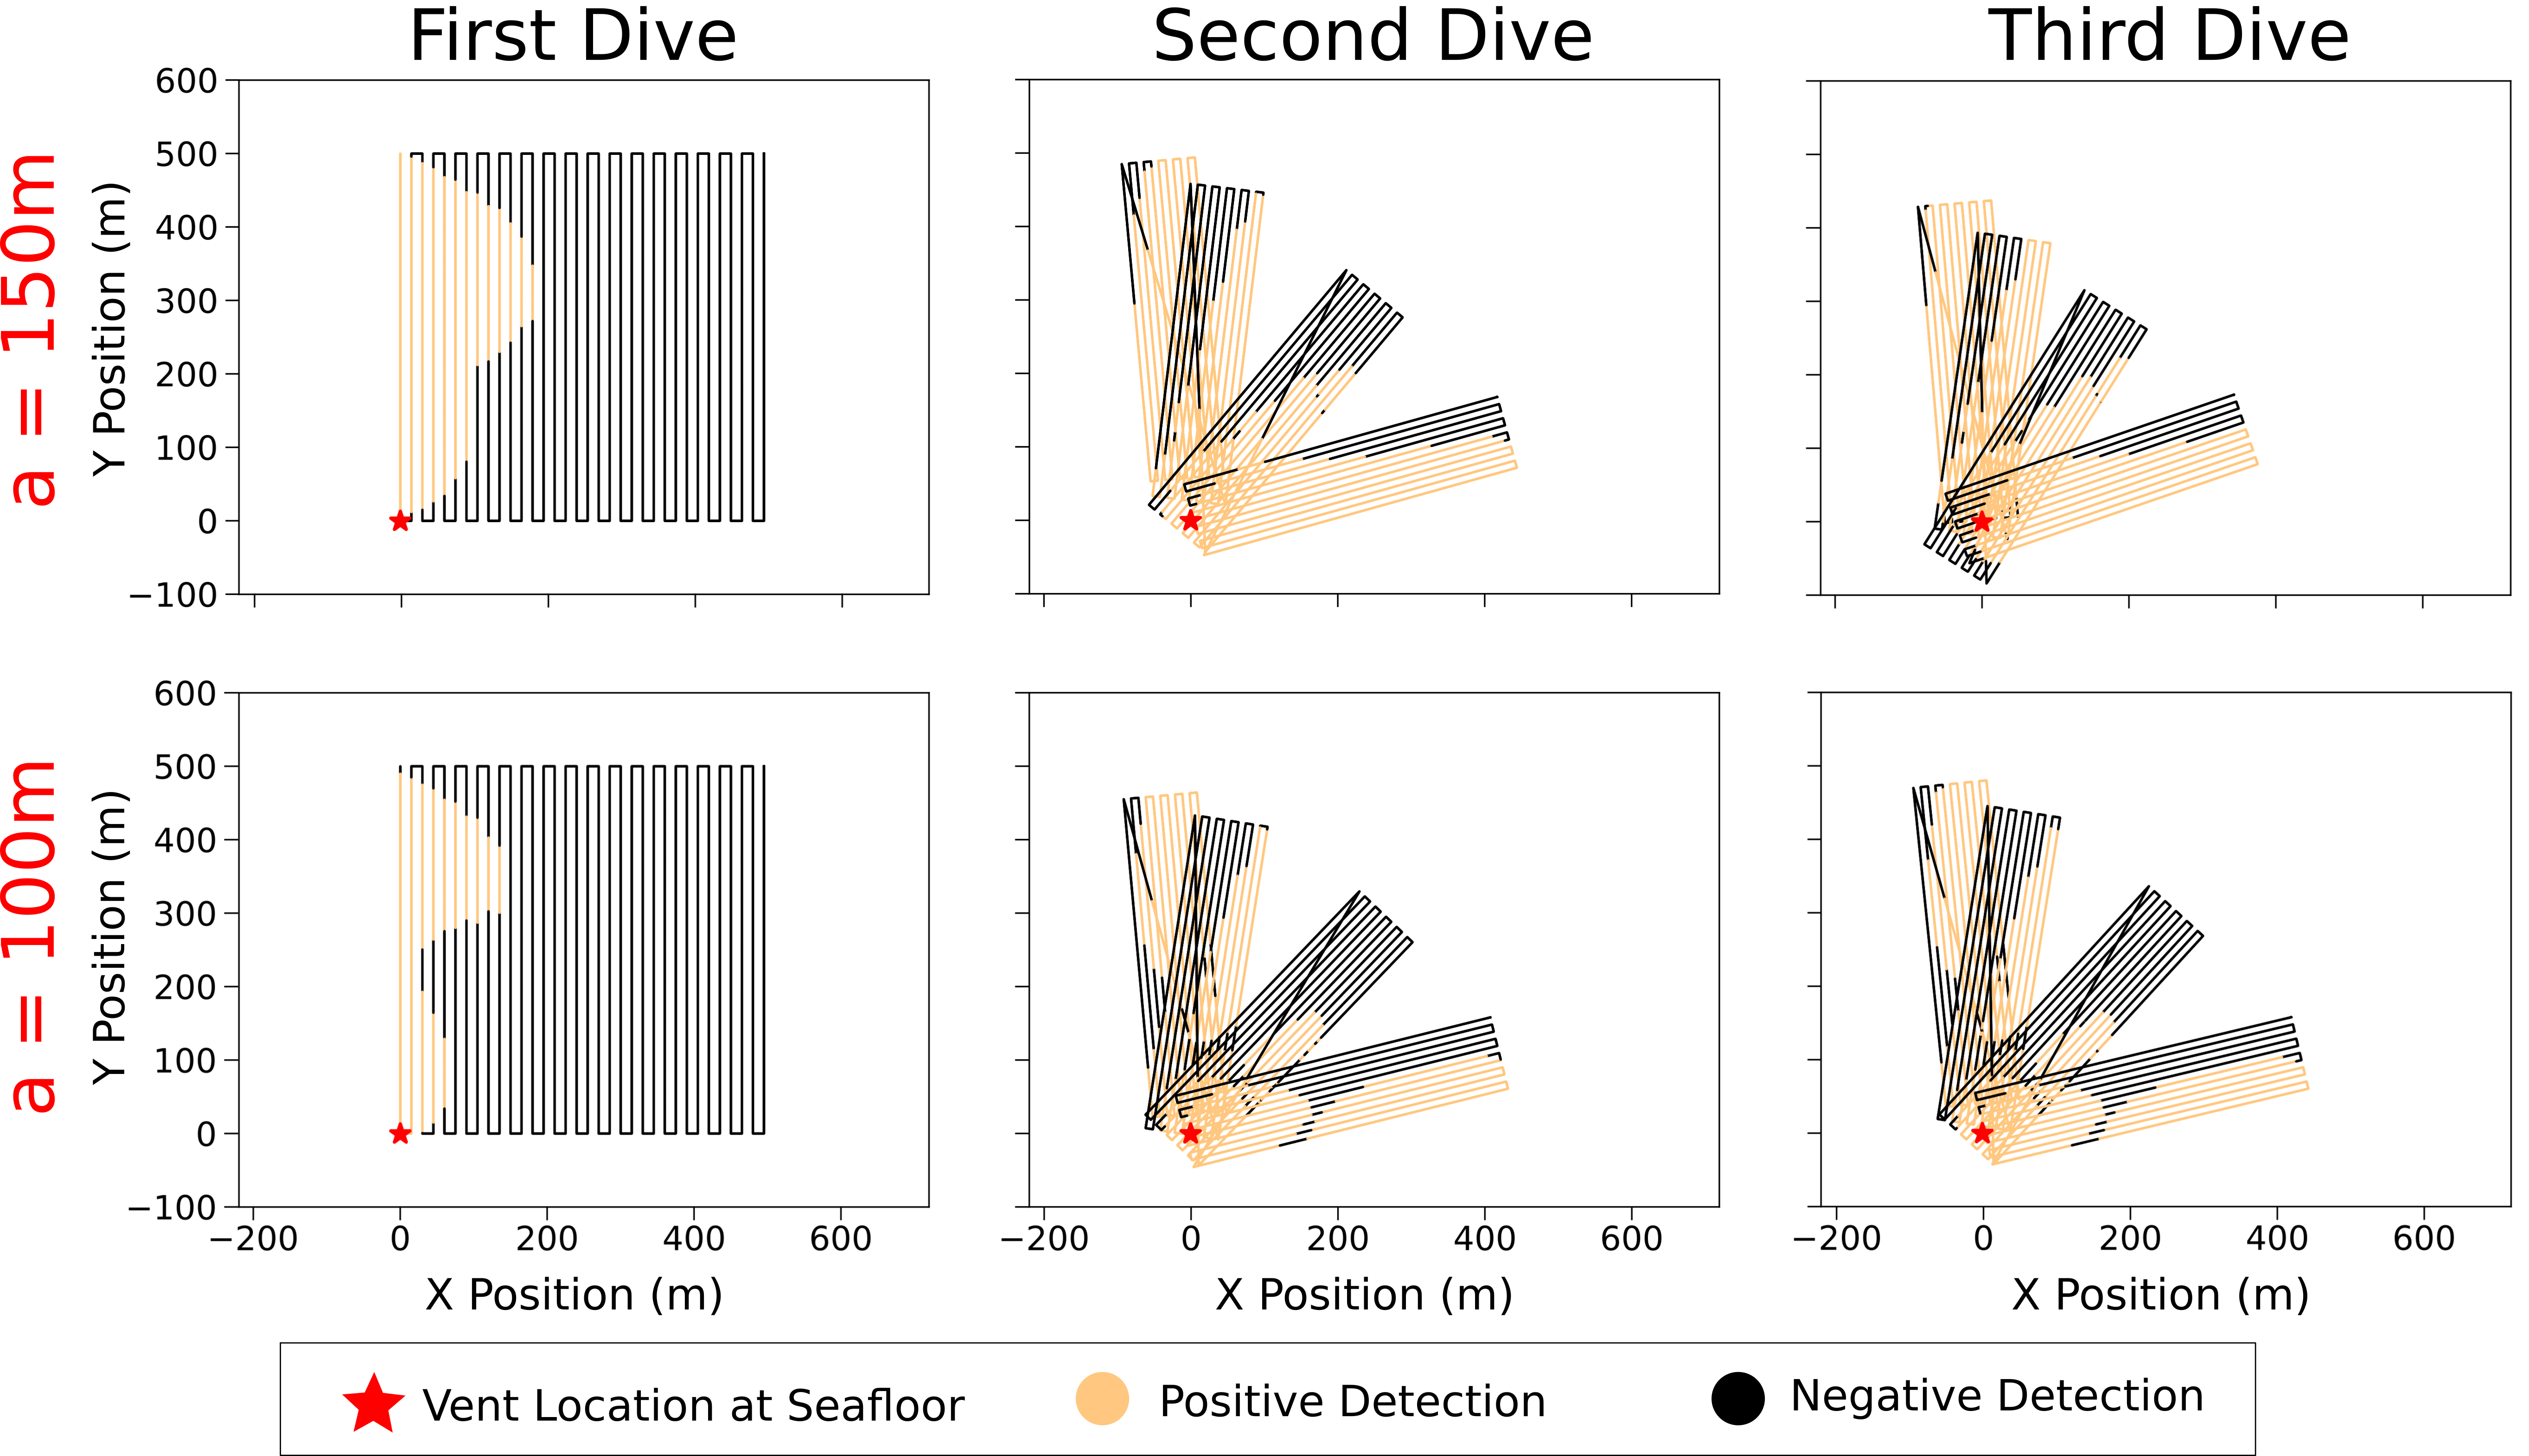
\includegraphics[width=0.85\columnwidth]{figures/sim_traj.png}
    \caption{\textbf{Naive and \PHORTEX-designed trajectories.} Trajectory examples for altitudes of \SI{100}{\meter} and \SI{150}{\meter}. The first dive is always a naive lawnmower; the second and third dive are \PHORTEX designed trajectories. \PHUMES is incrementally trained after each dive on the binary plume detections shown in this plot, which are sampled every meter traveled along the trajectory.}
    \label{fig:sim_traj_example}
\end{figure}

\begin{figure}[h!]
    \centering
    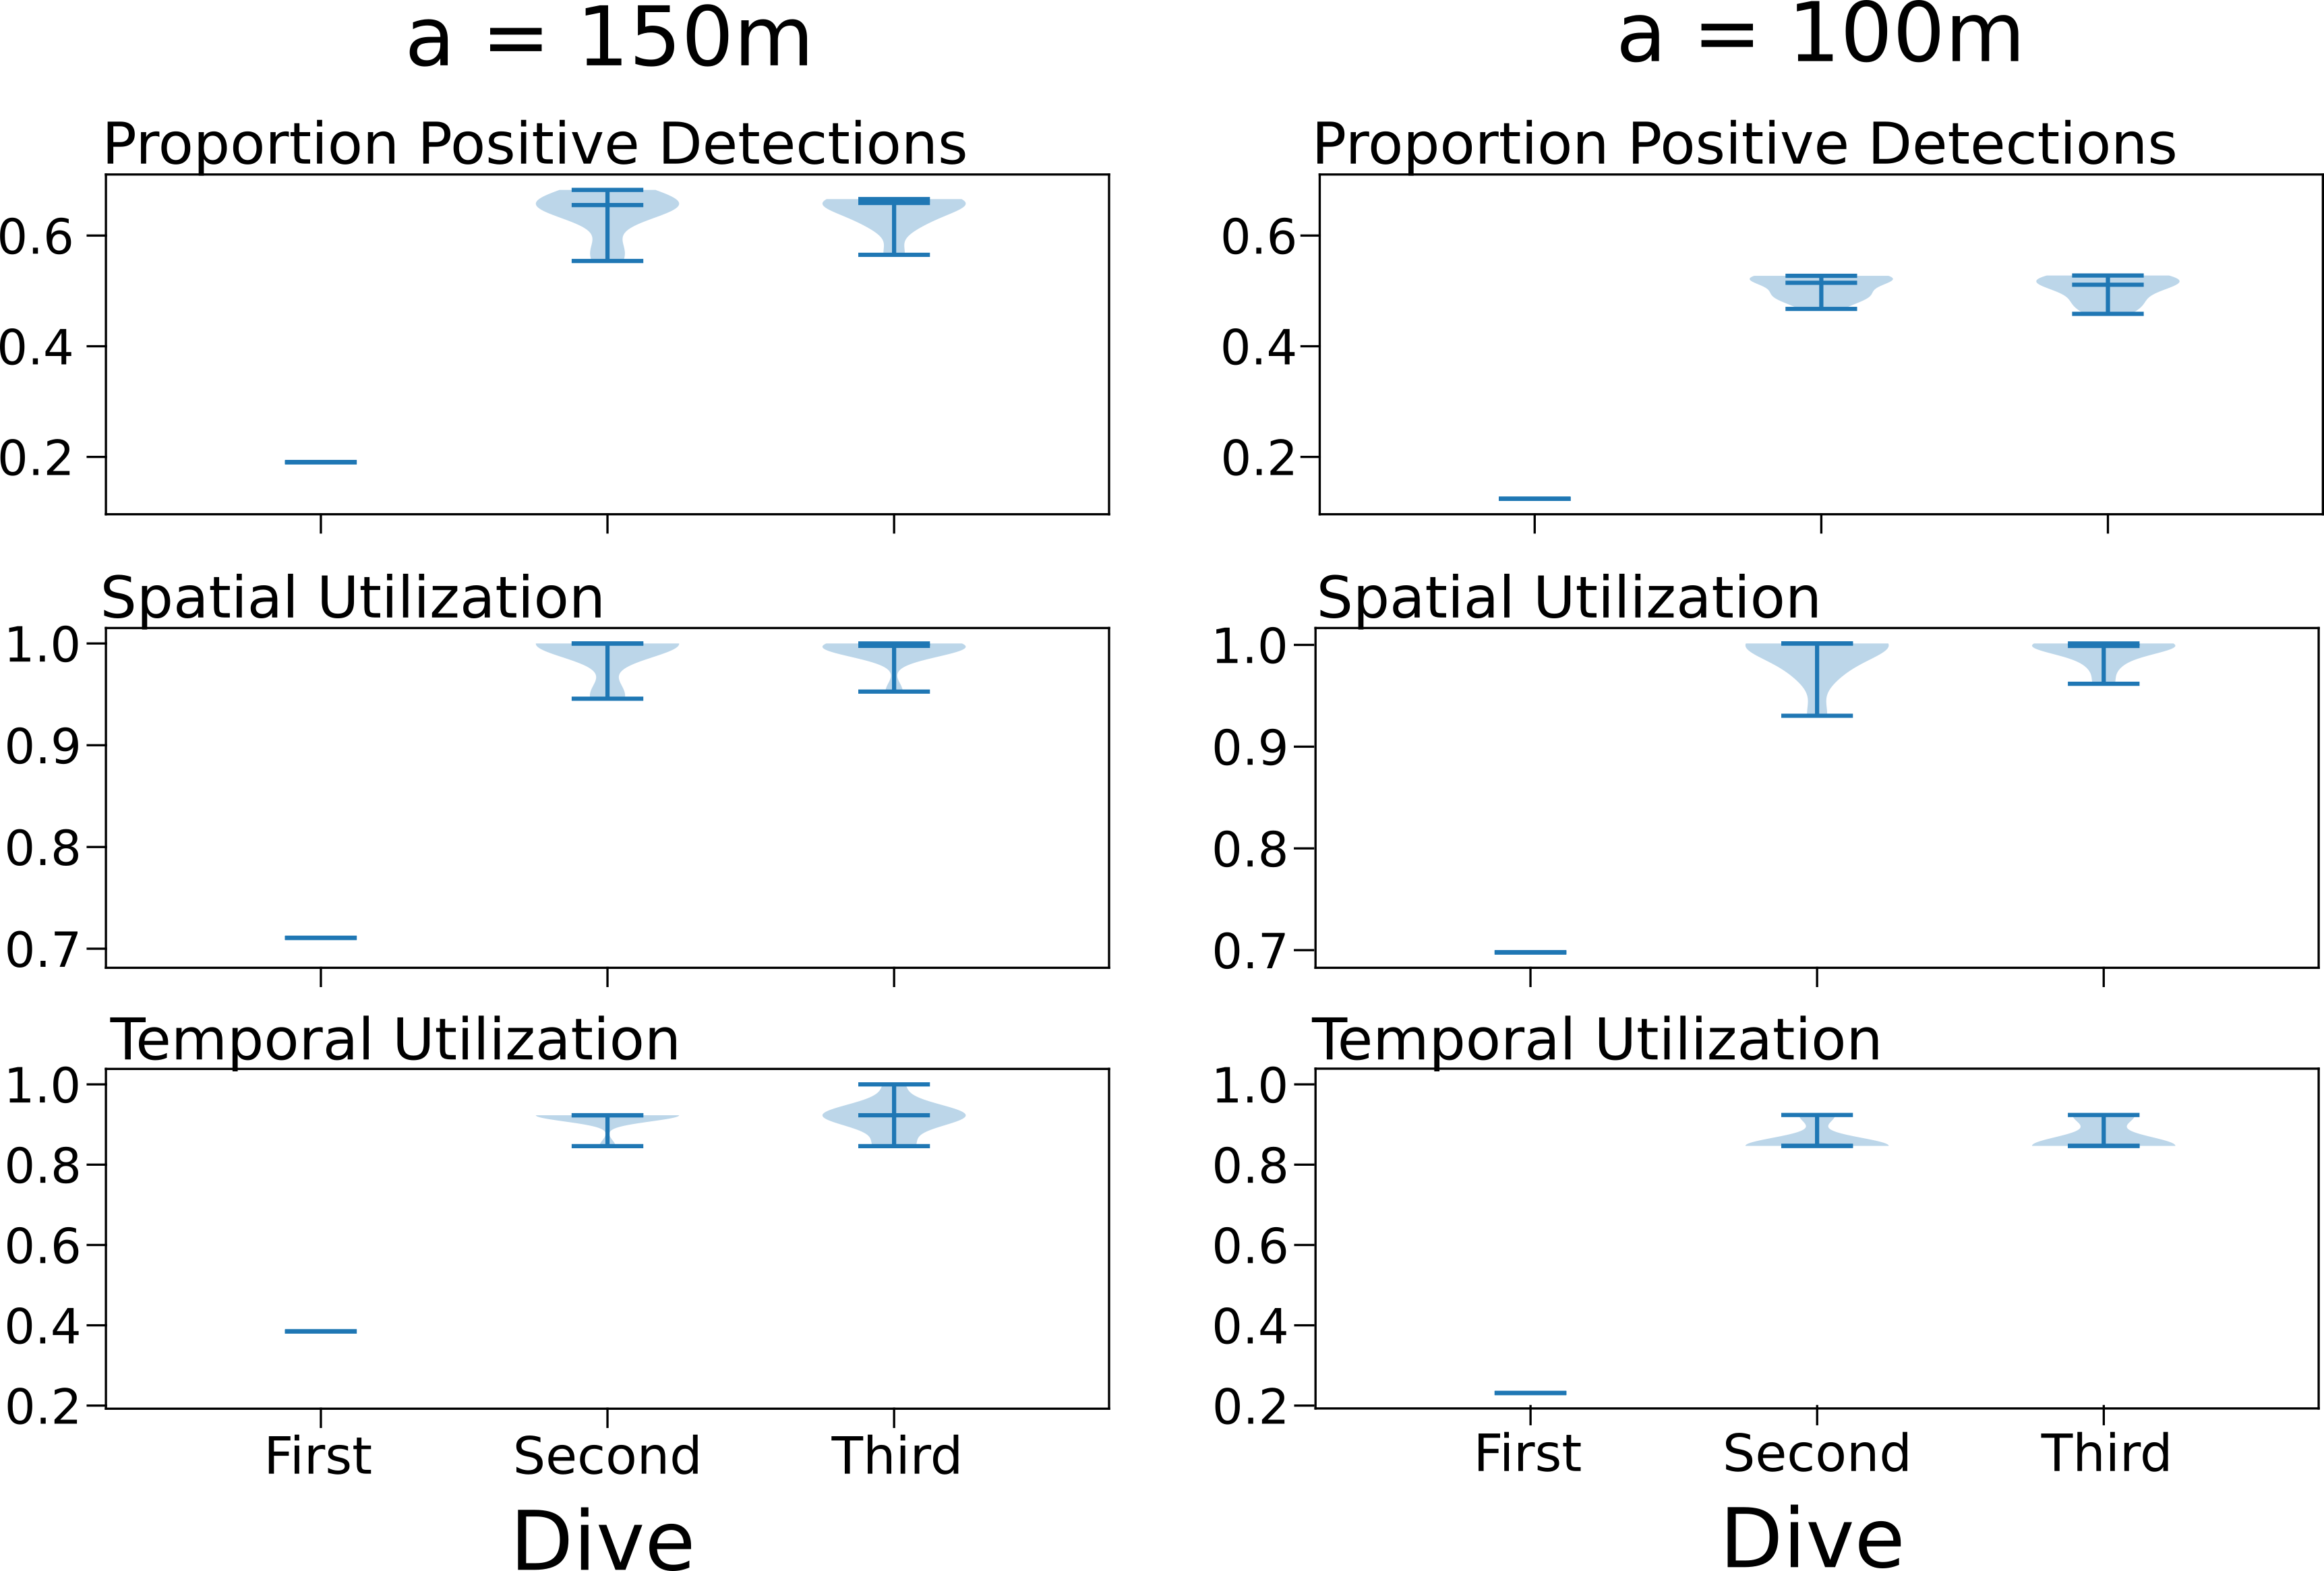
\includegraphics[width=0.75\columnwidth]{figures/sim_traj_performance.png}
    \caption{\textbf{Evaluation of the \PHORTEX trajectories.} The three-dive sequence, consisting of a naive lawnmower followed by two rounds of \PHUMES model training and \PHORTEX trajectory optimization, are evaluated for proportion of positive plume detections, spatial utilization, and temporal utilization (\cref{sec:eval_metrics}). The \PHORTEX-designed dives show a clear improvement in all three metrics, gathering more spatially and temporally diverse observations of the dynamic hydrothermal plume. Iterative rounds of \PHORTEX model-training and trajectory optimization continue to collect a high proportion of scientifically valuable observations.}
    \label{fig:sim_traj_perform}
\end{figure}


\paragraph{\PHUMES Model Validation}
The performance of \PHORTEX stays consistently high in the second and third dives, suggesting that \PHUMES quickly learns a sufficient model for planning from the small number of samples collected by the naive trajectories. To further understand the model learned by \PHUMES, we first qualitatively inspect the models learned by \PHUMES in two exemplar trials with data collected at \SI{100}{\meter} and \SI{150}{\meter} altitude during the initial naive survey of the first dive, as presented in \cref{fig:sim_model}. In the naive survey, less than 20\% of all detections are positive detections, and all detections only occur in the first 3 hours of the 12 hour mission. At an altitude of \SI{100}{\meter}, the robot essentially ``skims'' the bottom of the neutrally-buoyant plume; at \SI{150}{\meter}, the robot is consistently within the range of the neutrally-buoyant plume. Despite these altitude differences models learned in this example show remarkably similar characteristics---a predicted centerline no more than \SI{25}{\meter} off from the true environment's centerline, and a width that nearly completely envelopes the true plume distribution, which is promising for the context of planning missions. This is in contrast with an illustrative sample from the uninformative prior, which can arbitrarily produce plume structures that are significantly different in form from the true generating environment. It is also worth noting that despite training data only being available for 3 hours of the 12 hour simulated dive, the predictive quality of the model learned forecasts to an unseen time (t=9hrs) remains high. This largely demonstrates the advantage of using an embedded dynamics model in order to generate predictions of the state space to unseen times.

\begin{figure}[h!]
    \centering
    \includegraphics[width=\columnwidth]{figures/sim_mod.png}
    \caption{\textbf{Illustration of model learning.} Snapshots of the true generating environment are compared with an arbitrary sample from the prior distribution over \PHUMES parameters and the learned models from data collected by naive lawnmowers in both \SI{100}{\meter} and \SI{150}{\meter} simulation trials. In these two exemplar experiments, model learning performance is comparable between the \PHUMES models trained on data from different altitudes. The learned model, in comparison to the baseline sample, demonstrates a lower neutrally buoyant stem height, and is wider, and better explaining the data collected at the two sampling heights. Snapshots at different times show that the learned parameters robustly predict future shapes of the plume, even when trained on partial data available from the naive lawnmowers.}
    \label{fig:sim_model}
\end{figure}

To the quantify performance of the plume forecast generated by the MAP parameter sample after each trial, we compute the intersection over area (IoA) and intersection over union (IoU) between the true environment and each of the learned models after the naive and first \PHORTEX designed dives (\cref{fig:sim_phumes_perform}). A set of 10 parameter samples from the uninformative priors over the inference targets are used to generate an initialization performance distribution to show the breadth of forecast quality before any training. IoA (or recall) provides a number from 0-1 that expresses how many samples in the learned model are shared with the true generating environment. This number does not penalize false positives in the model: a value of 1 implies that all points in the model are contained by the environment, and a 0 implies that there are no points contained in the true environment. IoU (or precision) also provides a number from 0-1 that now penalizes false positives: a value of 1 implies perfect alignment between the model and environment, and a 0 implies no alignment. The comparison of these numbers helps to contextualize the performance of model learning. 

In \cref{fig:sim_phumes_perform}, we see that the learned models have a narrower performance window than the baseline samples, and that they generally exhibit very high IoA (up to 1), and a higher IoU (up to 0.9) than the baseline models (up to 0.75). With a high IoA, we can be confident that the learned models are placing value in areas for which there is plume, and with a higher IoU, we can be confident that the structure of the predicted regions with high value align well with the true environment. Taken together, a very high IoA with medium to high IoU suggest that trajectories planned with the \PHORTEX-trained models are very likely to plan for and successfully execute intersections with the targeted plumes, which is advantageous for our scientific task. We do not see a degradation of performance with different observations available between dives, suggesting that from very little data (a single naive dive), we can train an immediately useful model. Additionally, we note that there is a distinct difference in the distribution shapes of IoA and IoU between the altitudes across these trials. In particular, training from samples at \SI{150}{\meter} appears to be more consistently highly performant (IoA mode is at or near 1; IoU distributions skew towards 0.8) than at the lower altitude, which has a more distributed performance characteristic (with IoA skewed just about 0.8, and IoU centered just above 0.6). This has interesting implications for choosing deployment altitudes in practical missions, within the constraints of robot abilities (for instance, AUV \Sentry cannot swim over a certain altitude and maintain good localization, thus constraining what parts of a plume may be accessible in field deployments). We leave as future work the finer scale characterization of informativeness of different plume regions for model recovery in scientific settings.


\begin{figure}[h!]
    \centering
    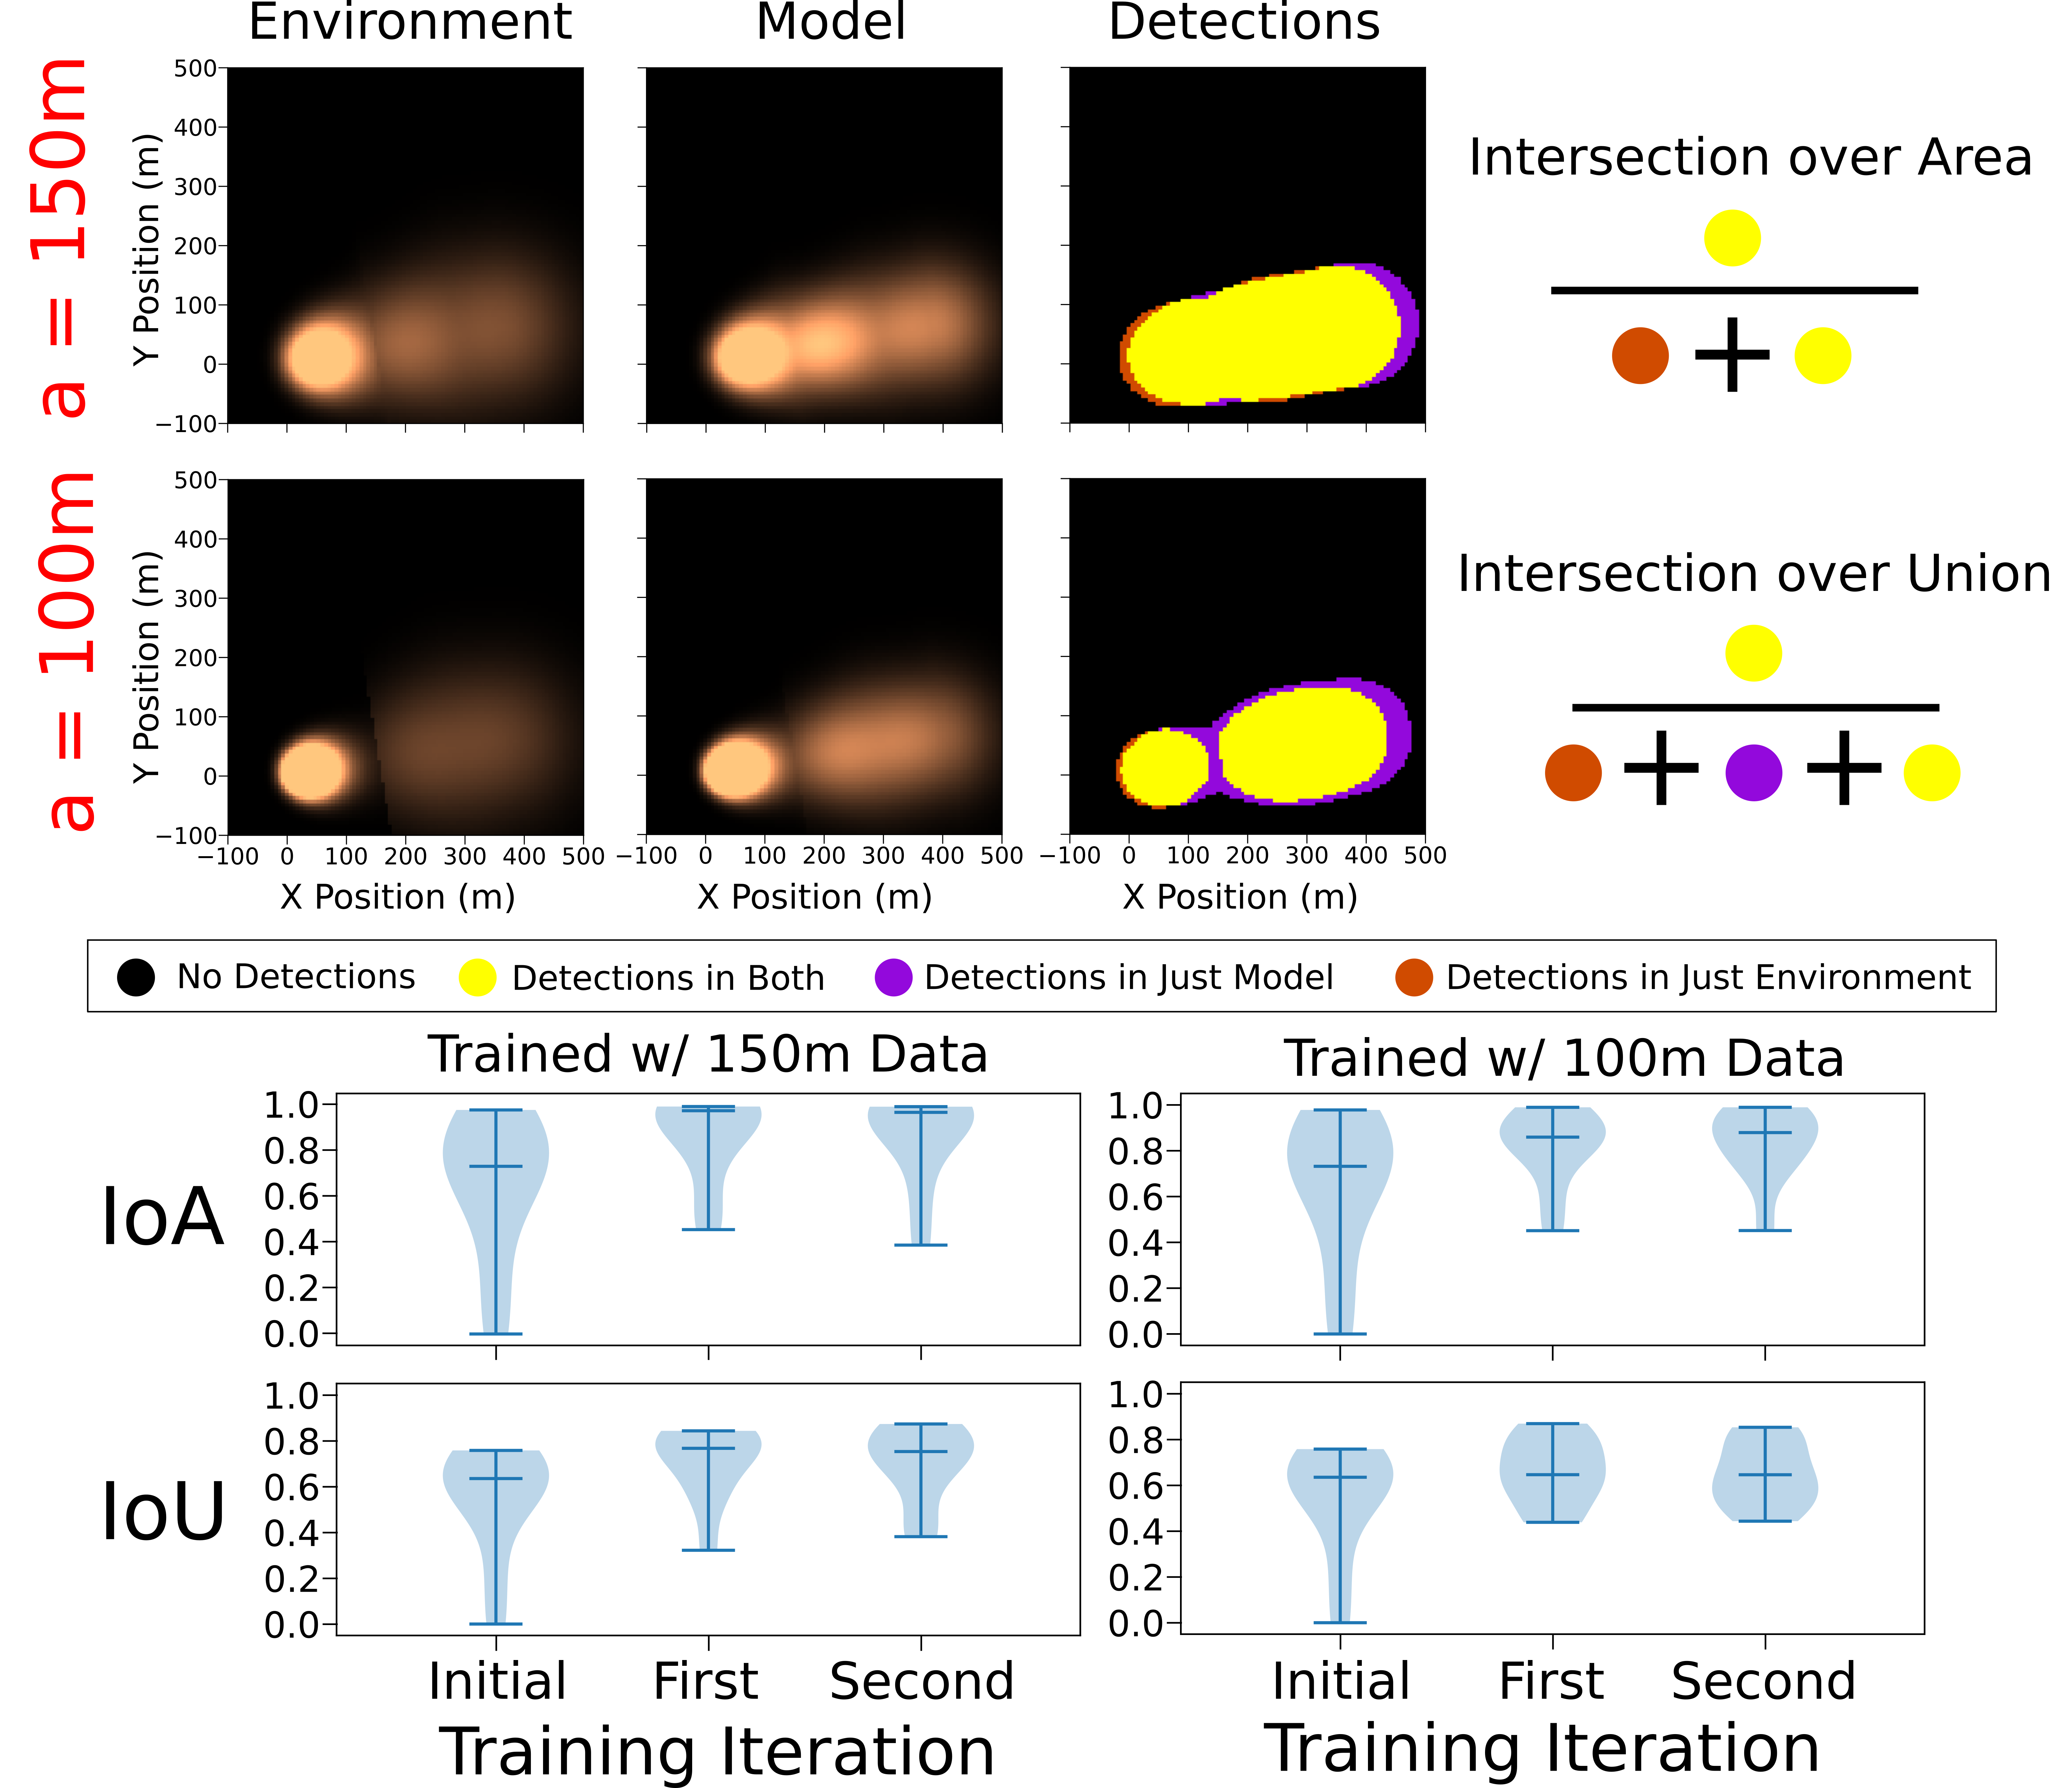
\includegraphics[width=0.9\columnwidth]{figures/sim_mod_performance.png}
    \caption{\textbf{Intersection over Area (IoA) and Intersection over Union (IoU) of trained models.} For each of trials trained from data at \SI{100}{\meter} and \SI{150}{\meter} altitudes, we compute the average IoA and IoU (using the method illustrated at the top) for a set of initial model samples (Initial), \PHUMES trained on the naive dive (First), and \PHUMES trained on the follow-up \PHORTEX-designed dive (Second). In general, we see the each of the iterative trained dives maintains similar performance; with high IoA and medium-to-high IoU that is consistently higher than initialized samples. Trials trained on data from \SI{150}{\meter} tend to have more performant model estimates (IoA near 1, IoU skewed above 0.8) compared to those trials trained on data from \SI{100}{\meter}.}
    \label{fig:sim_phumes_perform}
\end{figure}

% \begin{itemize}
%     \item We will first demonstrate \PHORTEX within the simulator we've created for generating plume funnels. We will show how \PHUMES converges to estimates of the true underlying distributions of initial conditions and parameter settings with and without noise. We will ideally show a graph that is RMSE of params versus mission iteration, and show a steep drop in error with steady improvement are iterations increase (fewer than 10 iterations will be graphed). 
%     \item We will additionally show performance on several key metrics, including reward versus iteration, total in-plume samples/accumulated reward under different model settings (e.g., number of samples in \PHUMES MCMC chain, prior uncertainty), and model mean and variance with each iteration. 
%     \item We will then show how sensitive trajectory optimization settings/chains are to collected reward, intending to show the advantage of using chains over a single highly-resolved lawnmower, at minimum.
%     \item If there is interest/time, we will then show how \PHORTEX performs in a numerically realistic simulator (as provided by our collaborator at University of Washington) and compute similar statistics as those indicated above. This addition would be used to demonstrate the complex real-time structure of plume snapshots, and show how the method generalizes to this setting. \VP{note that this is only if there is time; currently planning on only using the field results to demonstrate this, and may save simulation work for later tag-along conference/workshop paper}.
% \end{itemize}


\subsection{Field Trials with \PHORTEX at Sea}
In November 2021, \PHORTEX was used to design trajectories for AUV \Sentry at the Northern Guaymas Basin in the Gulf of California. Four deployments of AUV \Sentry were available to study the hydrothermal site. These deployments represent a planning spectrum, from fully human-designed surveys to fully \PHORTEX designed. We label the four deployments as follows:
\begin{itemize}
    \item \textbf{Dive H-Multi}: human designed, multi-task survey. This was the first deployment of \Sentry and the survey was designed to both attempt to find plume fluids and to bathymetrically map the local basin area (the map of which would be used as part of the safety check protocol for future deployments). This dive is representative of a standard nested strategy, in which progressively more targeted (finer resolution) surveys are used to study areas of interest. The dive was designed by a human expert who only had access to the approximate location of the target vent. The deployment lasted 21.3 hrs and collected 76,604 observations total.
    \item \textbf{Dive H-Plume}: human designed, plume-charting survey. This was the second deployment of \Sentry and the survey was hand-designed by the science party onboard the vessel to find and sample plume fluids. The science party had access to the performance of \Sentry in Dive H-Multi. The strategy was to sweep the basin above areas with known hydrothermal vents, and fly out into the basin in the direction that the plume fluids would be expected to advect. The deployment lasted 21 hrs and collected 75,430 observations total.
    \item \textbf{Dive HP-Plume}: hybrid human and \PHORTEX plume-charting survey. This was the third deployment of \Sentry and the survey consisted of trajectories designed by \PHORTEX trained by observations collected only in Dive H-Multi. Two of the trajectory primitives designed by \PHORTEX were replaced by ``naive'' lawnmowers placed over the known vent at two different times in the deployment. The deployment lasted 22.2 hrs and collected 79,792 observations total. Of these, 8.2 hrs and 29,438 observations were collected via the naive strategy.
    \item \textbf{Dive P-Plume}: \PHORTEX plume-charting survey. This was the fourth and last deployment of \Sentry. The survey was fully designed by \PHORTEX using observations only from Dive H-Multi, several days prior to this dive. The deployment lasted 9.9 hrs and collected 35,755 observations total. This deployment is notably much shorter than the other deployments due to increasing time constraints as the expedition was coming to a close. This deployment also used \Sentry in a ``depth-hold'' mode: whereas in all other dives \Sentry's depth followed the basin terrain, in this experiment the robot held an absolute depth.
\end{itemize}

\subsection{Field Trials with \PHORTEX at Sea: Results}
Using the metrics introduced in \cref{sec:eval_metrics}, we evaluate each of the four dives executed at sea to chart the space-time dynamics of a real hydrothermal plume as presented in \cref{tab:field_results} and visualized in \cref{fig:field_results}. Each dive took place at different times in the tidal cycle, on different days, and often at different altitudes in the water column, and thus the total plume samples available to collect during each dive is variable. With this in mind, we present and evaluate each dive quantitatively, and additionally qualitatively examine each as a case study for how different sampling paradigms perform in the real-world. There is no ground-truth available for the deep sea plume-charting problem; we evaluate each \Sentry dive assuming that the binary detections produced by the method in \cref{sec:sensor_models} are honest representations of the presence or absence of hydrothermally-derived fluids in the basin. 

The results of the field deployment in \cref{tab:field_results} demonstrate that \PHORTEX performs comparably to science expert-designed trajectories in the proportion of samples that are collected during dives, and importantly improves upon the spatial utilization (increasing both the range of the most distal plume detection and effectively utilizing of the entire explored range). This is most evident in the HP-Plume dive, in which the human designed portion is a naive lawnmower placed ``on top'' of the vent; the \PHORTEX-designed trajectory collects samples over twice as far from the plume source. Absolute temporal utilization is similar to human surveys; however the distribution of detections within the temporal utilization windows is improved --- for human surveys, detections tend to be ``bunched'' to either the first half (as in H-Plume) or second half (as in H-Multi). We see this most sharply in HP-Plume, in which 90\% of positive detections collected by the human-designed survey occurred only in the second of the two lawnmowers, from hours 20-23. In contrast, \PHORTEX designed trajectories collected detections more uniformly over the entire dive.  \cref{fig:field_results} shows the qualitative structure of each dive and showcases the diversity in the resulting datasets.

% Evaluating the efficacy of human- and \PHORTEX-designed trajectories in charting the space-time dynamics of a real-world hydrothermal plume is challenging. Unlike the simulation experiments, there is no ground-truth plume chart available and evaluating the counterfactual --- if \PHORTEX had gone here instead, how many more observations of the plume would have been collected? if we had used a naive planner instead of \PHORTEX for this deployment, how many fewer observations of the plumes would we have?--- is not straightforward. Due to operational constraints and the value of ship time, using an entire deployment of \Sentry to implement a lower-performing baseline is prohibitively wasteful; each deployment attempts to make the best use of available data to accomplish the task of plume charting.  In the remainder of the section, we evaluate each \Sentry dive using the metrics introduced in \cref{sec:eval_metrics}, assuming that the binary detections produced by the method in \cref{sec:sensor_models} are ground-truth detections and non-detections. 

% We look at several key metrics for each deployment: proportion of positive plume observations, utilization of spatial extent, and utilization of temporal dive window. The first metric, proportion of positive plume observations, is simply the number of observations collected in a dive that were classified as in-plume by the binary sensor model we describe in \cref{sec:sensor_models}. The second metric attempts to show how spatially effective the design of the survey was by first showing the absolute range that positive detections were made as a measure of distance from the chimney vent location and second showing how that range fit with the overall design of the survey. For example, if detections were made up to 300 m away from the vent, but the robot traveled up to 1 km away, then the survey spent too much time outside of the detectable plume region and would not be as effective as a survey that only traveled 200 m away but stayed well within the detectable plume range. Finally, the last metric is a measure of how effective the survey was at \emph{staying in} or \emph{revisiting} a plume over time. Given the duration of these missions, it is important to use the entire mission window for the task at hand; moreover temporally ``diverse'' observations are of scientific interest generally. We report the proportion of dive hours with at least 10\% or more positive detections.



\begin{table}[h!]
    \centering
    \begin{tabular}{c|c|c|c|c|c}
        Dive & Duration & Total Obs. & Prop. In-Plume & Spatial Util. & Temporal Util.  \\
        \hline
        H-Multi & 21.3 hrs & 76,604 & 22.3\% & \SI{300}{\meter} (19\%) & 9-17,20-21 (52\%) \\
        H-Plume & 21 hrs & 75,430 & 10.9\% & \SI{900}{\meter} (64\%) & 2,5-8,10-11,15-16 (43\%) \\
        \hline
        HP-Plume & 22.2 hrs & 79,792 & 41.8\% & \SI{600}{\meter} (100\%) & 1-3,5,7,11-23 (81\%) \\
        HP-Plume (H) & 8.2 hrs & 29,438 & 42.3\% & \SI{250}{\meter} (100\%) & 5,7,20-23 (75\%) \\
        HP-Plume (P) & 14 hrs & 50,354 & 41.5\% & \SI{600}{\meter} (100\%) &  1-3,11-20 (93\%)\\
        \hline
        P-Plume & 9.9 hrs & 35,755 & 12.8\% & \SI{450}{\meter} (100\%) & 1,5,8,9 (40\%)
    \end{tabular}
    \caption{\textbf{Per-dive statistics for field trials of \PHORTEX.} The spatial utilization is reported as both the most distal plume detection (measured from the plume origin) and the ratio of the most distal plume detection over the farthest distance that the robot traveled from the plume origin. Temporal utilization shows both which hours contain at least 10\% positive plume detection and what fraction of the total deployment duration contained such detections. The deployment HP-Plume is broken further into human designed (H) and \PHORTEX designed (P) portions for direct comparison.}
    \label{tab:field_results}
\end{table}

\begin{figure}[h!]
    \centering
    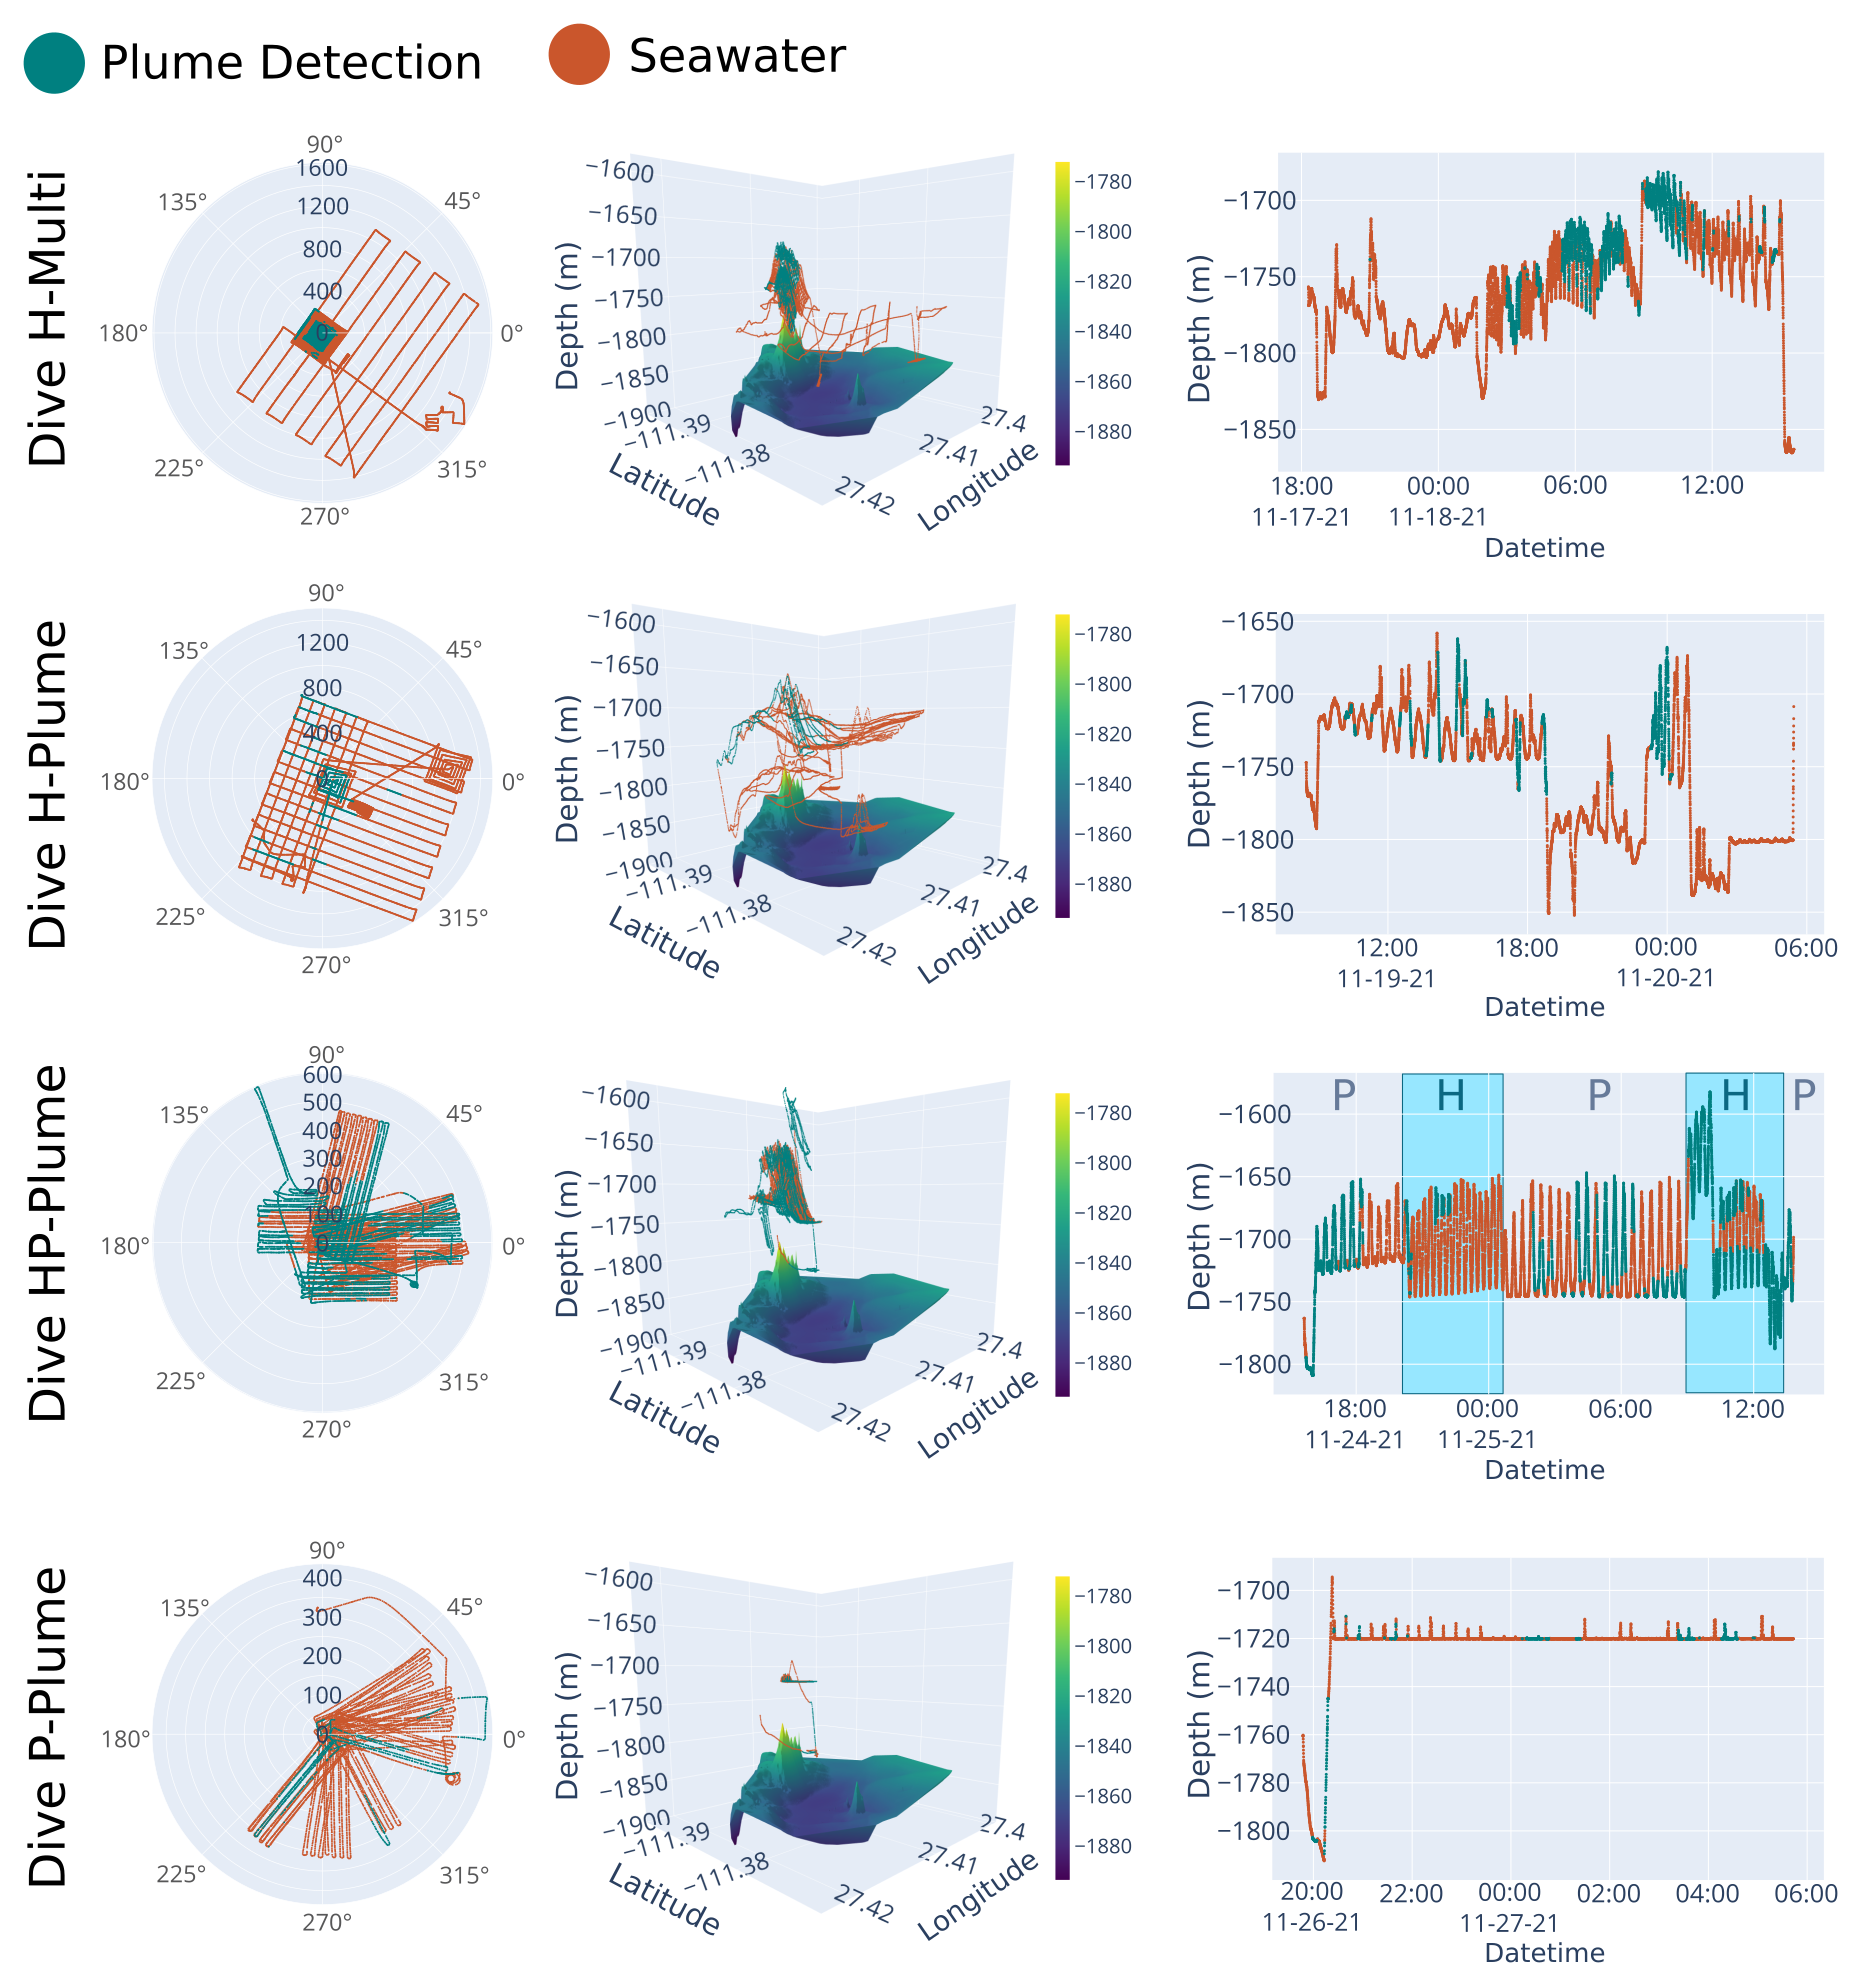
\includegraphics[width=1.0\columnwidth]{figures/detections_data.png}
    \caption{\textbf{The four field dives of AUV \Sentry.} All data is plotted according to its detection identity (in-plume or seawater). The first column shows a top-view of the dive trajectories in polar coordinates, in which angle and radius is computed relative to the chimney coordinate of the vent of study. In the center column, the 3D path of the vehicle over the rendered bathymetric terrain is provided. All but Dive P-Plume were dives conducted in altitude-hold mode with \Sentry, and so the trajectories show obvious changes in elevation; in contrast Dive P-Plume was held in depth-hold mode, so most observations are gathered within a depth-plane. The final column shows a time series versus depth of the detections collected. In Dive HP-Plume the portions of the dive that were human-designed and \PHORTEX-designed are labeled with H and P, respectively. As can be seen in the Dive HP-Plume time series, the two human-designed trajectories have significantly different performance, despite being in locally similar regions of the spatial domain. }
    \label{fig:field_results}
\end{figure}

In this field deployment, we demonstrate that \PHORTEX is a useful and practical tool for plume-charting. The performance of trajectories designed with \PHORTEX are comparable to those designed by human experts with key improvements in spatial and temporal utilization. It is further worth highlighting that \PHORTEX was trained only on data collected during the first dive, H-Multi, and reasonable performance during P-Plume using week-old training data emphasizes the long-range forecasting ability of the approach. Practically, the automated nature of \PHORTEX operationally alleviates significant decision-making burden on a science team and the trajectory-design burden on the \Sentry team; the ability to ingest data from external sensors and previous \Sentry missions, and produce trajectories that can be seamlessly ingested by the safety checking system without human intervention is of considerable benefit in the field. Moreover, the intermediate products of \PHORTEX, such as \PHUMES forecasts, are useful for other tasks in field operations, such as deploying other instruments or prioritizing instrument deployment order based on temporal changes in the environment by virtue of yielding rich context easily interpretable by the science team. 

% Similarly, \PHORTEX is trained on significantly less data than what the human experts had access to throughout the cruise; this emphasizes the advantage of the model-based, data-aggregation approach in \PHUMES. 

\paragraph{\PHUMES Validation with Basin Observations}
While there is no external ``ground-truth'' that we can use to evaluate the performance of \PHORTEX, we can compare the \PHUMES model trained on external and binary \Sentry observations with snapshots of the vertical distribution of turbidity near the hydrothermal ridge to get a sense for the utility of the \PHUMES model. After training, \PHUMES estimated the fluid exit velocity from the target chimney to be \SI{0.58}{\meter\per\second}, the vent area to be \SI{0.82}{\meter\squared}, and the vertical and horizontal mixing coefficients to be 0.15 and 0.19, respectively. Simulating these conditions with an initial vent temperature of \SI{340}{\celsius} and salinity of 34.908 PSU under a nominal crossflow of \SI{0.11}{\meter\per\second}, we compare the time-averaged plume height and width with the turbid intrusion that is observed in vertical casts of a shipboard rosette. The rosette was lowered and raised through the water column using a cable and winch on the ship; several vertical transects were collected over the course of the research cruise at the target autonomy site in addition to other sites throughout the basin. In \cref{fig:field_valid} we show two vertical transects, one conducted about \SI{100}{\meter} from a known vent, and one conducted \SI{600}{\meter} from the same vent. We see that within the model regions for predicted plume intrusions in the water column, strong turbid signals are observed in both vertical transects. This is indicative that the learned \PHUMES model is capable of uncovering the structure of the hydrothermal plume and lends confidence that the model is informative for planning sample trajectories that will intersect with plume fluids.

\begin{figure}[h!]
    \centering
    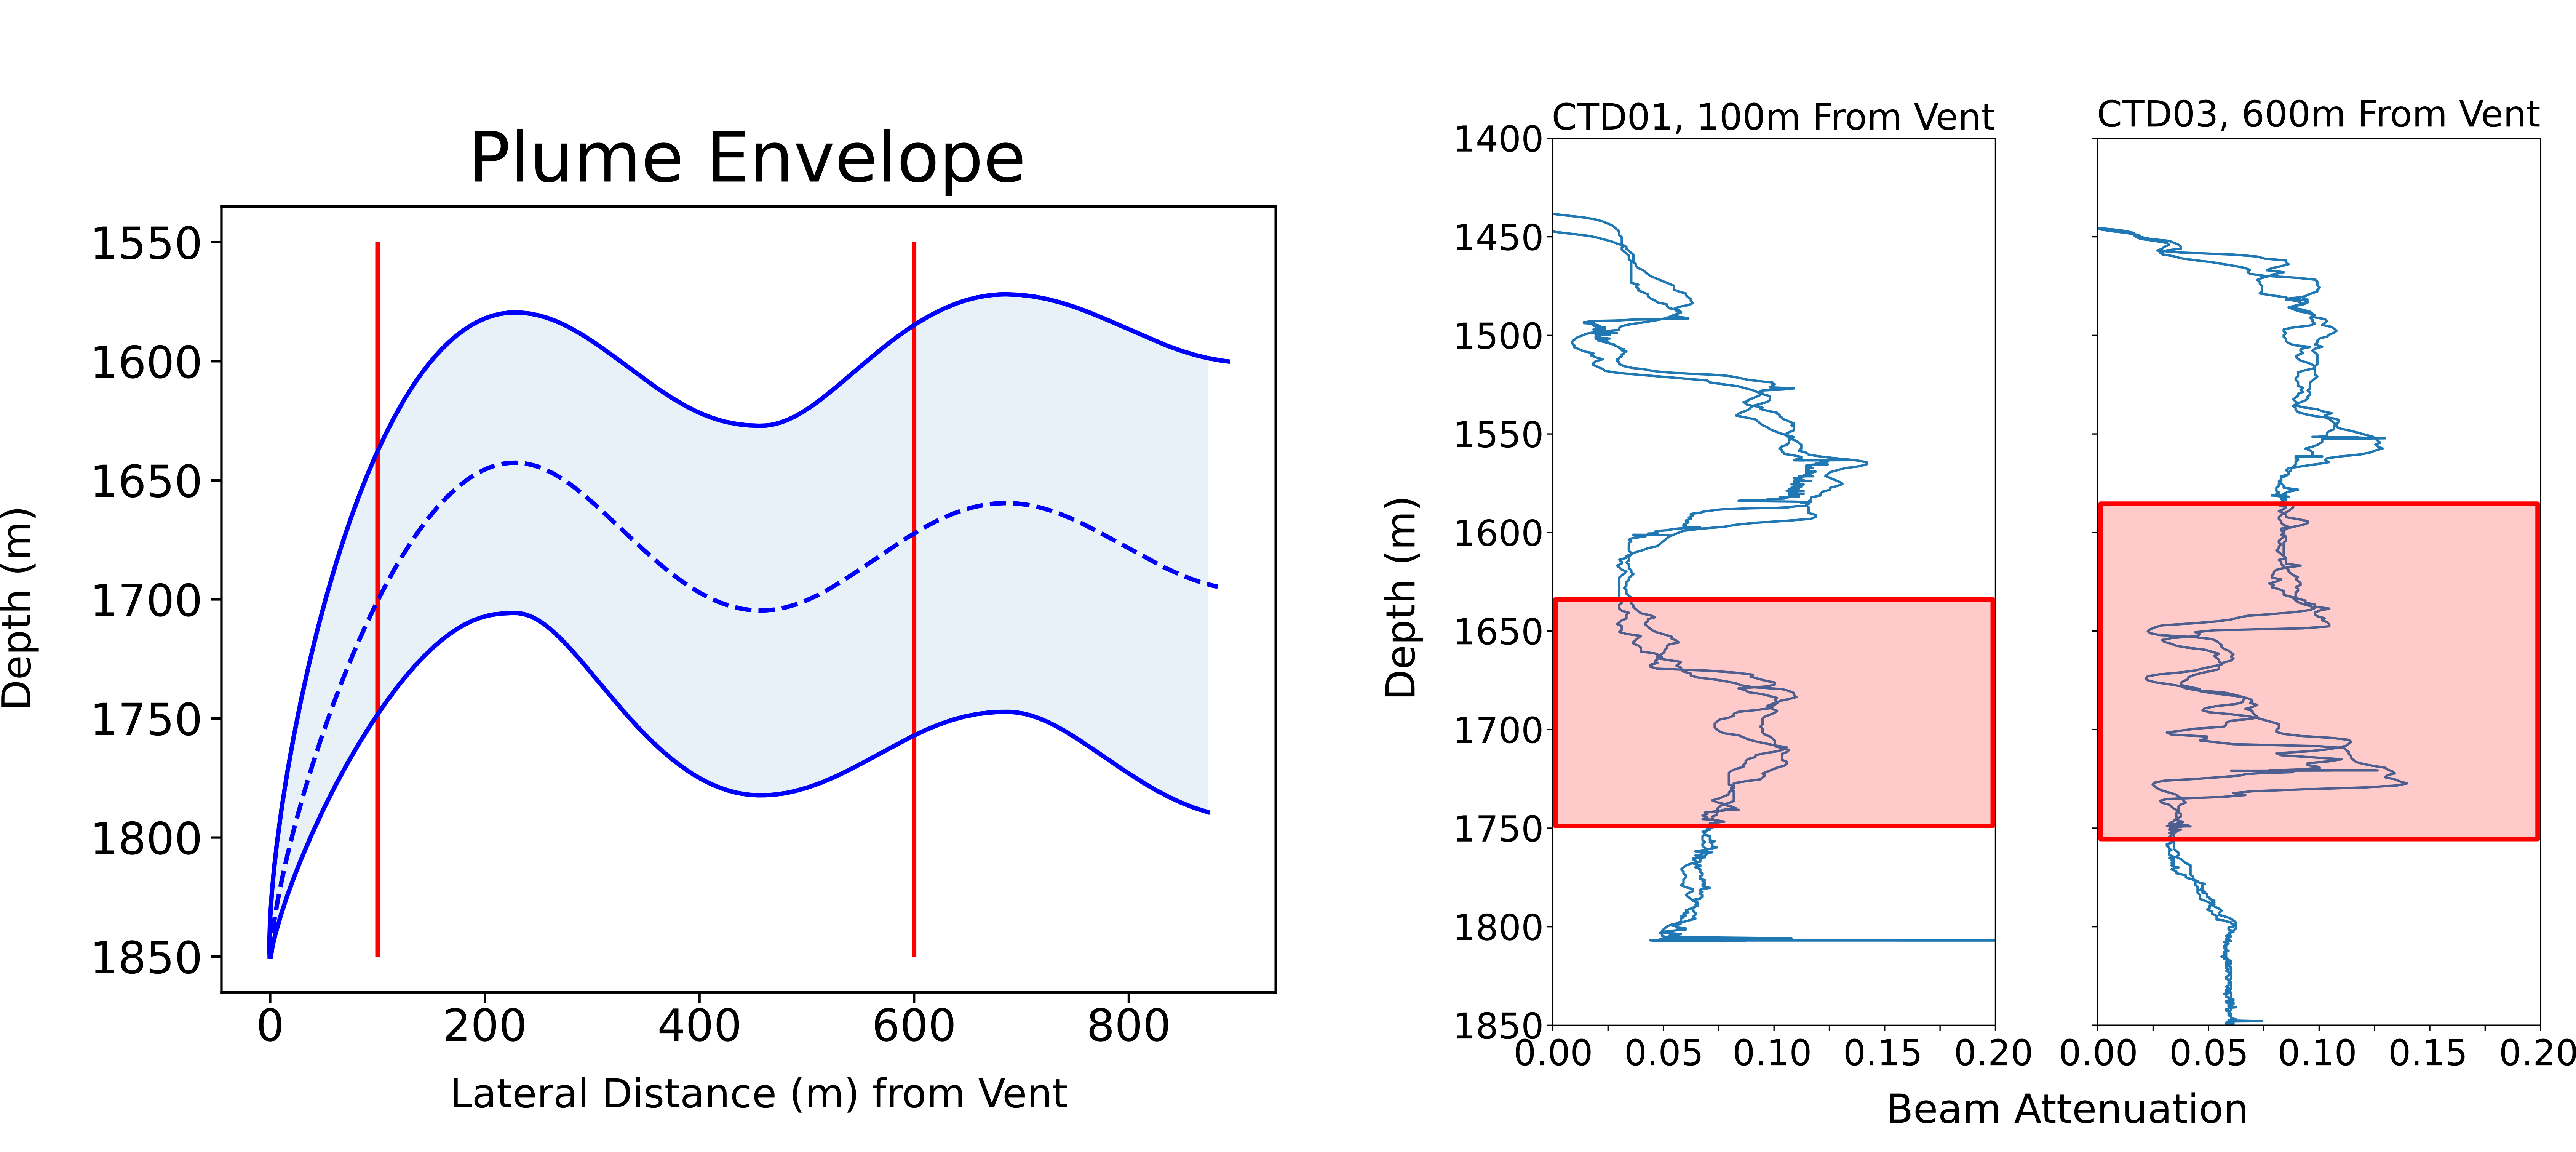
\includegraphics[width=1\columnwidth]{figures/field_validation.png}
    \caption{\textbf{Validation of \PHUMES model trained at sea.} We compare the nominal plume estimate from \PHUMES trained on at-sea data and \Sentry observations with vertical transects of turbidity from shipboard rosette. The plume envelope is the average plume estimated by \PHUMES for a nominal crossflow of \SI{0.12}{\meter\per\second}. Vertical red lines mark \SI{100}{\meter} and \SI{600}{\meter} laterally from the originating vent, for which vertical CTD casts were conducted. The region that the model estimates containing the lowest plume intrusion in the water column is highlighted on the turbidity transects. There is agreement between the model estimate and the transect data on the location of this turbid layer.} 
    \label{fig:field_valid}
\end{figure}


% \td{Note that this section is under construction! An overview of what this section will entail is below!}

% \begin{itemize}
%     \item This section will primarily present 4 trials that we performed while at sea -- 1 designed completely by hand, 2 partially designed by a person and by \PHORTEX, and one completely designed by \PHORTEX. The intent is to show the ``planning spectrum'' from fully-human to fully algorithmic, and comment on the form of these plans and their relative efficacy. Note that because the conditions between each iteration are different, the iterations are themselves not necessarily directly comparable (as in, claiming that one is ``better'' than another may be...bold) so we will be primarily focused on general metrics across all dives.
%     \item The Planning Spectrum: \begin{itemize}
%         \item We will show each of the 4 dives from fully human-designed to fully algorithmically designed. We will point out how the form factor between the lawnmowers/lawnmower chains differ, highlighting in particular how algorithmic chains tend to be strongly impacted by estimated crossflow, causing the trajectories to ``fan'' out; whereas human design trajectories tend to be conservatively placed centered at a known source.
%         \item We will show each of the four dives in both space and time; this will allow us to mark-up the figures and show where and when detections were made. We will ideally show that algorithmic trajectories tend to have more evenly distributed detections throughout a dive. We will also hopefully show that algorithmic trajectories tend to have more ``far afield'' positive detections of plumes.
%     \end{itemize}
%     \item Quantitative Results: \begin{itemize}
%         \item Some quantitative results we will share for each dive will include proportion of total samples in plume, proportion of total samples within/outside a certain radius from a known vent, RMSE of estimates vent characteristics by \PHUMES (train a naive \PHUMES model from observations collected by each dive, how to the dives inter-compare? How does it compare with estimates from ROV \emph{JASON}? How does a per-dive iteration look?)
%     \end{itemize}
% \end{itemize}
  % observations + PHUMES part of JFR paper
  % \chapter{Physically-Informed Operational Robotic Trajectories for Scientific Expeditions}
\label{chap:phortex}

\begin{center}
    \begin{minipage}{0.7\textwidth}
      \begin{small}
        Now it would be very remarkable if any system existing in the real world could be exactly represented by any simple model. However, cunningly chosen parsimonious models often do provide remarkably useful approximations...For such a model there is no need to ask the question ``Is the model true?''. If ``truth'' is to be the ``whole truth'' the answer must be ``No''. The only question of interest is ``Is the model illuminating and useful?''.\\ \emph{George Box}
      \end{small}
    \end{minipage}
    \vspace{0.5cm}
\end{center}


On expeditions, quality observations of water column properties and their anomalies are strong evidence used by a science party to strategically plan research activities---deployment of certain instrumentation or platforms (where, when, why), allocation of resources to different projects, and scheduling for high-stakes one-off missions. \cref{chap:afar} showed how to parse scientific instrumentation data for hydrothermal plume identification by domain experts to assist in data discoverability and interpretation. These tools provide descriptive snapshots of what was observed during a mission, but rely on the science experts to extrapolate these snapshots into future mission states. This chapter directly addresses how to recover a predictive model of plume state from partial observations collected from heterogeneous sensors, and formulates an automated routine for leveraging this predictive model to design dense charting surveys with AUV \Sentry. %Content from this chapter is directly adapted from~\cite{preston2022physically}.

\section{Introduction}
Transient, dynamic phenomena---deep-sea hydrothermal plumes, algal blooms, warm core eddies, lava flows---are of interest in many disciplines of observational science. \emph{Expeditionary science} encapsulates the observational sciences that require \emph{in situ} sample collection of environmental phenomena for scientific discovery and model development. In such cases, the environmental targets are typically impossible to observe using remote sensing (e.g., satellites) either due to desired spatial and temporal resolution, environment adversity (e.g., the deep sea, within closed structures), or the nature of the scientific target of interest and corresponding sensing equipment (e.g., building a taxonomy of algae requires physically processing water samples). Expeditionary science is, by definition, conducted in partially-observable and often dynamic environments; thus performing useful and effective data collection in expeditionary science poses a challenge for human and autonomous decision-makers alike.

In this chapter, mapping the space-time dynamics of deep-sea hydrothermal plumes using an autonomous mobile robot is studied. Deep-sea hydrothermal plumes are a source of chemicals and particulates that play a significant role in biogeochemical cycling in the deep ocean \autocite{le2019hydrothermal,resing2015basin,dick2013microbiology, vic2018dispersion, scholz2019shelf}. Understanding the fate of chemicals and particulates in hydrothermal plumes is of significant interest to biogeochemists and physical oceanographers; however, directly studying plumes in the water column is a substantial challenge. Chiefly, deep-sea plumes have complex dynamics in space and time---advective forces (e.g., deep currents, topographic updrafts), diffusion, and turbulent mixing act on plumes as they rise through the water column. A robot tasked with charting a plume must be able to forecast where and when it will intersect with different regions of the plume in order to collect useful observations of its spatiotemporal structure, but the underlying dynamics of a plume are uncertain as these forces are generally unobserved. The problem is exacerbated by the inherent challenge of sensing a plume using chemical sensors --- the chemical distribution of a plume can only be observed with point sensors and no single point measurement is sufficient to locate the plume.

In addition to the technical challenges of determining a sensing strategy for a highly uncertain and dynamic phenomena, the deep-sea environment ($>$\SI{200}{\meter} depth) can only be accessed by depth-capable equipment that are often significantly constrained by operational and safety policies. For example, autonomous underwater vehicles (AUVs) in this setting are typically restricted to execute preset trajectories hand-designed by human scientists (e.g.,~\cite{camilli2010tracking}). In this mode, the AUV cannot react to measurements while executing the set trajectory. Such ``open-loop'' trajectories can result in sparse measurements of a target phenomenon, such as a dynamic plume, or can miss short-lived events entirely \autocite{flaspohler2019information, preston2019adaptive}. However, this open-loop concept of operations remains the state-of-the-art in practical deep-sea science because preset trajectories are easy to encode, do not require extensive on-platform computing resources, and result in predictable robot actions that can easily be supervised. Here, constraints introduced by a specific robot, the AUV \emph{Sentry}, are considered. \Sentry is operated by the National Deep Submergence Facility (NDSF) at the Woods Hole Oceanographic Institution (WHOI) \autocite{kaiser2016design} and by operational policy is typically only permitted to execute pre-determined regular trajectories like ``lawnmower'' patterns or spirals, making online adaptation impossible. %However, given the cost of scientific field operations and the value of the data collected, it is critical to improve the efficacy of robots like \Sentry as scientific tools. 

Enabling depth-capable robots such as \Sentry to perform expeditionary science and study spatiotemporal phenomena using preset, non-adaptive behaviors requires an autonomy system that can design fixed trajectory patterns strategically to maximize desirable intersections with a dynamic phenomena. To strategize effectively, this autonomy system should learn to forward-simulate the dynamics of the target environment over a long-horizon from a small history of robot deployments and plan subsequent deployments using these predictions. This is fundamentally a \emph{sequential decision-making problem}, and is closely related to informative path planning (IPP) problems, in which a robot selects behaviors according to an information-theoretic reward function using a probabilistic belief of the environment. Existing methods in IPP (e.g.,~\cite{Hitz2017,hollinger2013sampling,flaspohler2019information,levine2010information,binney2012branch}), the related field of experimental design and optimal sensor placement (e.g.,~\cite{Krause2008,wang2019reinforcement}), and general decision-making under uncertainty (e.g.,~\cite{sunberg2018online, somani2013despot,kocsis2006bandit,Silver2010}) have demonstrated that sequential decision making can be applied to sampling scenarios in which online, adaptive behaviors are possible, the phenomenon of interest is static, and/or there is an opportunity to train the belief model from many trials, multiple sensors, or highly adaptive trajectories. The assumptions made in each of these typical scenarios is violated in the expeditionary science sampling problem, and this chapter proposes an autonomy framework, \PHORTEX: \phortex, that addresses each of these constraints with the set of algorithmic choices made for the observational model, belief representation, and planner within the framework (\cref{fig:intro_summary}). 


\begin{sidewaysfigure}
    \centering
    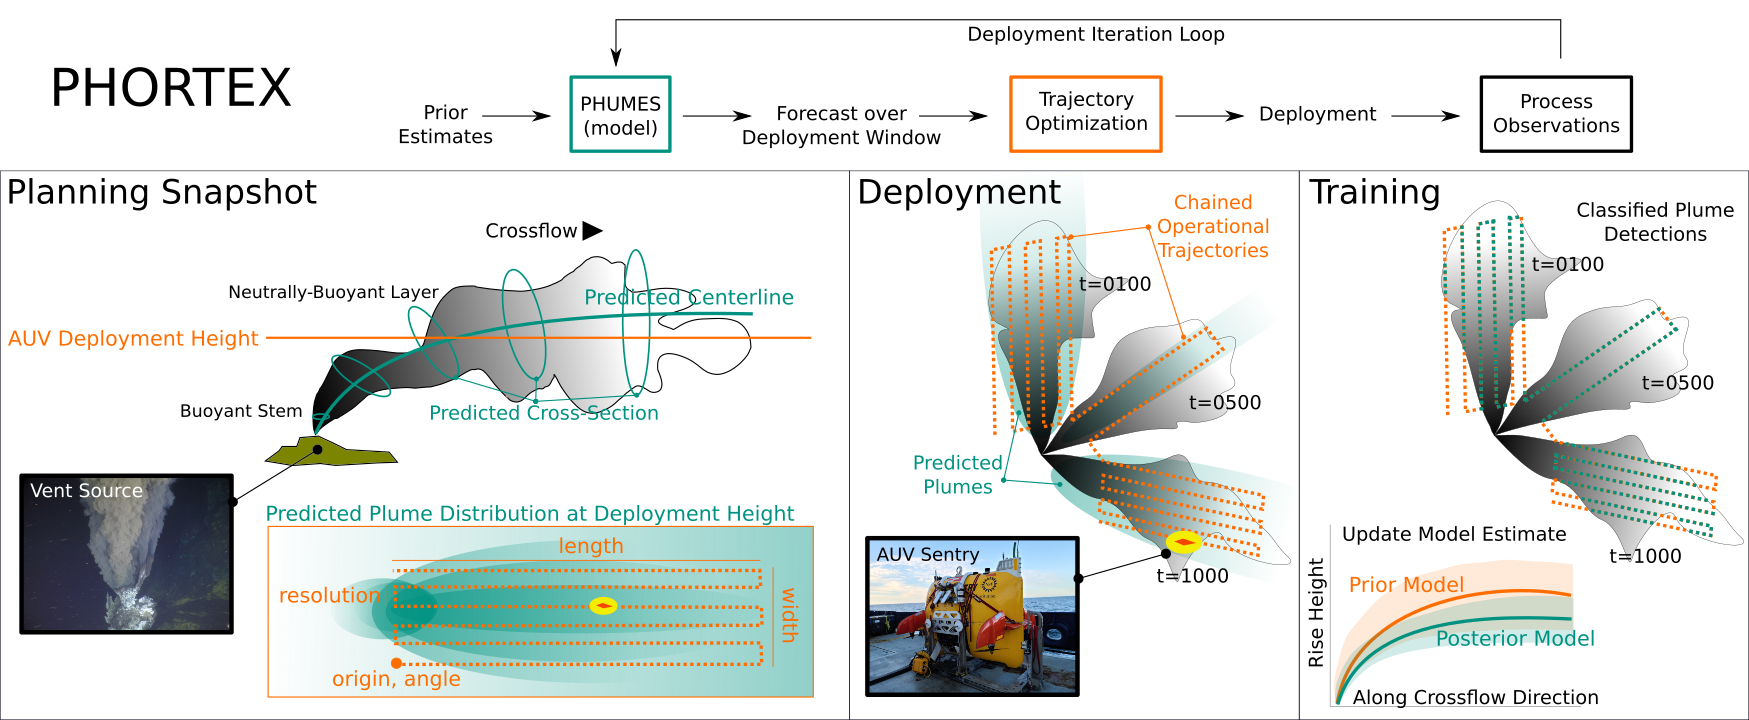
\includegraphics[width=\columnwidth]{figures/summary_intro_figure.png}
    \caption[An overview of \PHORTEX: \phortex.]{\textbf{An overview of PHORTEX: \phortex.} Over the course of an expedition, AUV \Sentry may be deployed several times. In preparation for a deployment, the belief model \PHUMES: \phumes is used to generate a probabilistic forecast of temporally-evolving plume centerlines and cross-sections from estimates of vent characteristics and fluid crossflow (e.g., current) which can be either seeded with prior information from scientific knowledge, data of opportunity from other deployed sensing equipment, or previous \Sentry deployments. A trajectory optimizer is given the forecasts and for a given altitude that \Sentry can operate, modifies the parameters of a ``lawnmower'' trajectory primitive (height, width, origin, orientation) to maximize expected in-plume samples. Several lawnmowers are chained together to form a complete deployment trajectory and ``chase'' the moving plume distribution throughout the deployment area. \Sentry executes the trajectory and following a \emph{Sentry} deployment, observation locations are classified as binary plume detections from analysis of several science sensors. This product is then used to update the \PHUMES model of plume centerline and cross-section over time. The new \PHUMES model is then used to plan the next deployment of \Sentry.}
    \label{fig:intro_summary}
\end{sidewaysfigure}


%%%%%%%%%%%% Contributions
\subsection{Contributions}
In this chapter, the autonomy system \PHORTEX is formulated to solve the hydrothermal plume charting problem under operational constraints imposed by a state-of-the-art AUV, \Sentry. \Sentry, by policy, can only execute pre-defined trajectories while underway, and can only be deployed a small number of times during a given expedition. As modern IPP, plume-hunting, and front-tracking techniques strongly rely on underway adaptive behaviors, these frameworks are extended for \Sentry by formulating a \emph{deployment-by-deployment} sequential decision-making problem which treats each pre-defined deployment of \Sentry as a single action in sequence with few steps. Each deployment action is defined as a chain of operationally-approved trajectory primitives (i.e., lawnmower patterns), which are parameterized by a small number of characteristics including their relative size, resolution, and position, and are optimized to collect the most number of expected in-plume detections.

To represent the robot's knowledge (belief) in order to optimize a given chain for tracking a target plume, a probabilistic model \PHUMES: \phumes is introduced, which provides long-horizon forecasts of plume state. As very few deployments of AUV \Sentry are possible during an expedition, \PHUMES must overcome the challenge of sample-efficient dynamics learning from sparse, partial observations. To do so, the existence of well-characterized analytical models for buoyant plume dynamics used in ocean and atmospheric sciences is leveraged to embed a numerical simulator into a Bayesian filtering framework. The use of this simulator creates a strong inductive bias for the dynamics learning problem for a given field site. There are several advantages to this scheme: the forecasts generated by \PHUMES are driven by a set of physically-meaningful parameters (e.g., vent temperature, crossflow magnitude) which are interpretable by the science team and over which the science team may have useful prior knowledge; the \PHUMES framework can easily accept data or information external to \Sentry deployments that map to the physically-meaningful parameters; and forecasts that are generated support computation of many summary statistics (e.g., mean, variance), providing flexibility for defining reward functions for the trajectory optimization scheme.

Simulations demonstrate that \Sentry using \PHORTEX can collect more spatially and temporally diverse plume-derived fluid samples as compared with classical surveying approaches. The diversity of samples corresponds to observing more unique regions of a plume structure, and has important, positive implications for scientific inquiry to be performed on the dataset collected by \Sentry in post-expedition analyses, to be further discussed in \cref{chap:field_results}. 

The rest of this chapter is organized as follows: in \cref{sec:problem} the hydrothermal plume charting sequential decision-making problem is formally presented as a partially-observable Markov decision process (POMDP). \PHORTEX and \PHUMES, the algorithmic contributions for approximately solving the hydrothermal plume charting POMDP are presented in \cref{sec:methods}. \cref{sec:experiments} provides a description of a simulated deployment and experimental results are discussed in both \cref{sec:phortex_perform} and \cref{sec:phumes_perform}. In \cref{sec:phortex_future} future work related to the contributions of this chapter are discussed, and in \cref{sec:phortex_conclusion} some closing remarks are provided. 

\subsection{Advancing Hydrothermal Studies with Robots}
\label{sec:phortex_charting}
Hydrothermal vents, as described in \cref{sec:charting-plumes} and \cref{sec:rw_plumes}, produce warm, chemistry rich fluids that rise rapidly into the water column until reaching a point of neutral buoyancy with the ambient water, where the plume then spreads out in a neutrally-buoyant layer. When studying hydrothermal plumes, recovering location of the venting source, reconstructing the shape of the plume structure, and estimating energetic and chemical flux (e.g., heat output into the ocean), are key objectives.

A wealth of prior work has primarily focused on localizing hydrothermal venting plume sources (e.g.,~\cite{jakuba2007stochastic, mcgill2011robot, nakamura2013discovery, paduan2018discovery, mason2020evaluation, wang20203, kim2020discovery,ferri2010novel}) using a variety of equipment such as ship-based acoustics, towed instrument rosettes, remotely-operated vehicles (ROVs), human-occupied vehicles (HOVs), and autonomous underwater vehicles (AUVs). Specialized seafloor equipment is subsequently deployed at the inferred venting site to e.g., estimate bulk chemical or nutrient flux from the vent or characterize the driving magmatic system underneath the crust. Generally, vent localization approaches use detections of anomalous water masses (as determined from \emph{in situ} sensors) in the water column to constrain the location of a seafloor vent. The localization methods can be fully offline, in which surveys by vehicles like \Sentry with no adaptive capacity are post-processed and vent locations are inferred \autocite{jakuba2007stochastic,nakamura2013discovery}, or they can be fully online, in which autonomous gliders with adaptive capabilities utilize e.g., gradient descent to seek a plume source \autocite{wang20203}. In \autocite{branch2020demonstration}, an autonomous glider tasked with localizing a vent source adaptively chains uniform coverage trajectories with increasingly fine resolution as the robot position converges on an estimated vent location. This chaining is emulated in \PHORTEX, however the selection of trajectories is done completely offline before AUV \Sentry is deployed. Online strategies for hydrothermal plume hunting almost universally employ glider-type robot platforms, which are typically smaller, payload-limited, and less depth-capable than vehicles like \Sentry. 90\% of known vent fields are deeper than \SI{200}{\meter} in the ocean, and over 75\% are deeper than \SI{1000}{\meter} \autocite{beaulieu2013authoritative}. Gliders widely accessible to the research community are typically not rated deeper than \SI{1000}{\meter}, which means that deep-sea research is reliant on vehicles like \Sentry and demand advances in offline-suited planning techniques.

Also relevant to this study is ``plume hunting'' research in robotics, which has been equivalently styled as odor mapping, odor localization, source localization, and source seeking. In these works, the source emits a substance (e.g., gas, radio, acoustic, odor) and through partial observations of the emitted substance, the source is discovered using techniques that can be divided broadly into biologically-inspired heuristic search (e.g.,~\cite{reddy2022olfactory,chen2019odor}) or adaptive IPP (e.g.,~\cite{salam2019adaptive}). Biological or heuristic techniques, including gradient-based algorithms like chemotaxis \autocite{morse1998robust}, or algorithms that directly mimic a particular animal \autocite{edwards2001representing}, tend to be reactive and myopic. In contrast, adaptive IPP can be nonmyopic, and algorithmically tends to embed knowledge (either heuristically or rigorously) about flow-fields (i.e., advection and diffusion) to assist in plume localization. Such techniques also live on a spectrum, from algorithms that resemble biologically-inspired approaches like infotaxis \autocite{vergassola2007infotaxis} to methods that use model order reduction techniques to encode complex numerical models (e.g., Navier-Stokes equations) into a belief model to better treat complex data \autocite{peng2014dynamic}.

While source discovery remains an important area of research, in this chapter the focus is on how science can be advanced at the hundreds of vents that have been successfully identified. Thus, a complementary problem to source discovery is posed: \emph{given a venting source, what impact do the venting fluids have on the local environment?} In this framing, rather than using detections of a plume as a means of source localization, the detections themselves are the valuable data product for scientific inquiry. By placing instruments throughout an evolving plume structure over multiple length- (meter to kilometer) and time- (hours to days) scales to collect dense in-plume measurements, previously intractable questions with respect to microbial lifecycle and transport, carbon cycling, and anomalous water mass formation, can be approached. Work that has used robots to map or chart plume-like structures has been presented as the ``front-tracking'' problem \autocite{li2014multi,chen2019odor}. In this problem, two water masses converge (such as the warm hydrothermal fluid and the cold background seawater), and the goal is to use a robotic vehicle to track the edge of these water masses or stay within a single type of water mass. The importance of both multirobot collaboration and online decision-making in these schemes is essential to their efficacy; the research in this chapter is the first to present a water mass tracking solution within an offline optimization strategy with a single agent, and the first to attempt this for the hydrothermal charting problem.


%%%%%%%%%% Logistics
\subsection{Closing the Loop: Expedition Logistics}
Oceanographic research expeditions are an undertaking that requires the coordination and collaboration of a science party, external engineering teams that maintain and operate the scientific equipment used during studies, and the captain and crew aboard a research vessel (on which everyone lives and works during operations). Deep-sea ($>$\SI{200}{\meter} depth) capable robotic platforms used in oceanic research are assets independently maintained from a ship, and typically requested on a per-expedition basis. AUV \Sentry may be deployed on tens of expeditions in a given year, with up to 250 days at sea \autocite{kaiser2016design}. Safety of both people and equipment are held to the highest importance. Further, the critical role of \Sentry in oceanographic research drives the strict operational policies that dictate \Sentry deployments to prevent vehicle loss or damage.

It is with this context that \Sentry deployments are designed by the science party and ultimately approved by the \Sentry engineering team. In a typical workflow, the science party may provide a set of coordinates or waypoints they generate based on bathymetric maps, prior knowledge, or previous data (when available). The \Sentry team designs survey trajectories based on these coordinates and respecting basic operational constraints of the vehicle (e.g., speed, minimum/maximum altitude from the seafloor). With approval of the \Sentry team, science party, and captain, the survey is then executed. A single ``dive'' of \Sentry is multiple hours (typically not less than 5 hours, and under 24 hours). At the conclusion of a dive, \Sentry is recovered from the ocean and data products containing hundreds of thousands of point measurements from multiple heterogeneous sensors are made available to the science team within a few hours after \Sentry returns to the deck. Depending on the length of the dive, 12-18 hours of vehicle cycling time (e.g., recharging, instrument maintenance, preparation for the next deployment) are required. Based on the length of an expedition and other ongoing research activities, \Sentry may be deployed only a handful of times.

The complexity of these basic operations for \Sentry alone, in addition to the burden of coordinating several other ongoing scientific projects happening simultaneously, day-to-day operational changes, and unforeseen discoveries and hurdles, make performing ``closed loop science'' with robot platforms a challenge while at sea. For hydrothermal plume monitoring, a combination of sensor streams need to be used to make confident plume detections \autocite{jakuba2007stochastic}, but information about the exact tidal state, state of the venting source, and background sea characteristics are typically not provided in these products, and can require fusing data from other instruments deployed on a cruise, if available. The planning challenge is further exacerbated when the design of a new mission requires not just deep analysis of the collected data, but forecasting the implications of those data onto a new day, new site, or new objective. 

\PHUMES and \PHORTEX aim to alleviate the burden of closing the loop onboard a research vessel for AUV operations by generating interpretable phenomenon forecasts informed from diverse data streams and trajectories that can be verified by science party members and approved by \Sentry engineers. Algorithmically, the formulation of \PHORTEX as a sequential decision-making framework produces trajectories which are informed by previous observations, thus literally behaving like a closed-loop controller for robot actions. %Through a real field mission to the Gulf of California to chart hydrothermal plumes in the northern Guaymas Basin, we demonstrate how \PHORTEX can be practically deployed for plume charting.

\section{Problem Formulation}
\label{sec:problem}
During scientific expeditions, the objective of a robot is to collect useful measurements, as defined by a given task (e.g., reduce uncertainty over a quantity, find the global optimum in a distribution, track a moving target). For hydrothermal plume charting, the goal is to map or ``chart'' the spatiotemporal structure of a buoyant plume using a dynamically constrained AUV. Such a chart enables scientists to infer relevant scientific properties of generating vents (e.g., chemical flux) and to create detailed models of deep-sea interactions and nutrient cycling. This section describes how general problems in expeditionary science can be formulated as sequential decision-making problems, the specific constraints of AUV \Sentry and how they influence the sequential decision-making problem, and finally presents a formal description of hydrothermal charting as a partially observable Markov decision process. 

\subsection{Scientific Expeditions as a Sequential Decision-Making Problem}
Expeditionary science requires a robot to make a sequence of decisions to collect scientifically useful measurements of an unknown, partially-observable spatiotemporal environment under operational constraints. Generally, the expeditionary science decision-making problem can be formulated as a partially observable Markov decision process (POMDP). Let $\mathcal{P}(\cdot)$ denote the space of probability distributions over the argument. A finite horizon POMDP can be represented as tuple: $(\Ss, \A, T, R, \Zz, O, b_0, H, \gamma)$, where $\Ss$ are the states, $\A$ are the actions, and $\Zz$ are the observations. At planning iteration $t$, the agent selects an action $a \in \A$ and the transition function $T: \Ss \times \A \to \mathcal{P}(\Ss)$ defines the probability of transitioning between states in the world, given the current state $s$ and control action $a$. The transition function governs both how the state of the robot will evolve, given a chosen action, and the potentially stochastic evolution of the underlying spatiotemporal environment. After the state transition, the agent receives an observation according to the observation function $O: \Ss \times \A \to \mathcal{P}(\Zz)$, which defines the probability of receiving an observation, given the current state $s$ and previous control action $a$. The reward function $R: \Ss \times \A \to \reals$ serves as a specification of the task, assigning the states of the world that are useful for a given scientific objective high reward and others low reward. A POMDP is initialized with belief $b_0 \in \mathcal{P}(\Ss)$ --- an initial probability distribution over state --- and plans over horizon $H \in \integers^+$ with discount factor $\gamma \in [0, 1]$.

As the robot moves through the world, it selects actions and receives observations. Since the state of the world is not directly observable in a POMDP, the robot maintains a probability distribution over possible states (i.e., belief) and must update this distribution each time it takes an action and receives an observation. Given the transition and observation models, the belief can be updated directly using a Bayes filter \autocite{sarkka2013bayesian}:
\begin{align}
    \tau(b_{t-1}, a_{t-1}, z_t) = b_t
        &\defeq \mathcal{P}(S_t \mid a_0, z_0, \dots, a_{t-1}, z_{t-1}, z_t) \\
        &= \frac{\int_{s \in \Ss} O(s, a_{t-1}, z_t) T(s, a_{t-1}, s')b_{t-1}(s')}{\int_{s' \in \Ss} O(z \mid s', a_{t-1}) \int_{s \in \Ss} T(s' \mid s, a_{t-1})b_{t-1}(s)}
    \label{eq:bayes_tau}
\end{align}

\noindent where $\tau(b,a,z)$ is the updated belief after taking control action $a$ and receiving observation $z$ (Eq.~\ref{eq:bayes_tau}). Unfortunately, \cref{eq:bayes_tau} is often intractable to compute directly and an approximate Bayesian inference procedure is required to represent the belief (e.g., a Kalman filter \autocite{welch1995introduction}, a particle filter \autocite{Silver2010}, or variational methods \autocite{wainwright2002environmental,kucukelbir2017automatic}). 

Due to the stochastic, partially observable nature of current and future states, the realized reward in a POMDP is a random variable. Optimal planning is defined as finding a horizon-dependent policy $\{\mathcal{P}_t^*: \mathcal{P}(\Ss) \to \A\}_{t=0}^{H-1}$ that maximizes expected reward: $\mathbb{E} \Big[ \sum_{t=0}^{H-1} \gamma^t R\big(S_t, \mathcal{P}_t(b_t)\big) \mid b_0 \Big]$, where $b_t$ is the updated belief at time $t$, conditioned on the history of actions and observations. The recursively defined horizon-$h$ optimal value function $V^*_h$ quantifies, for any belief $b$, the expected cumulative reward of following an optimal policy over the remaining planning iterations: $V_0^{*}(b) = \truemax_{a \in \A} \mathbb{E}_{s \sim b}[R(s, a)]$ and
\begin{align}
    &V_h^{*}(b) =  \max_{a \in \A} \mathbb{E}_{s \sim b}[R(s, a)] + \gamma \int_{z \in \Zz} \mathcal{P}(z \mid b, a) V_{h-1}^*(\tau(b, a,z)) \ \text{d}z,
    \label{eq:value}
\end{align}
\noindent for $h \in [1, H-1]$.

The optimal policy at horizon $h$ is to act greedily according to a one-step look ahead of the horizon-$h$ value function. However, \cref{eq:value} is intractable for large or continuous state, action, or observation spaces and thus the optimal policy must be approximated. Much of the art of practical decision-making uncertainty is making well-designed algorithmic and heuristic choices that enable efficient and robust planning algorithms. %In the remainder of this section, we introduce the plume charting POMDP with AUV \Sentry and in \cref{sec:methods}, we describe the specific algorithmic choices that enable \PHORTEX to approximately solve it.  



\subsection{Scientific Decision-Making with AUV \emph{Sentry}}
There are several levels at which an AUV can behave autonomously. At the lowest level, an AUV is given navigation waypoints and executes a closed-loop controller and state estimator to drive to that waypoint; this type of autonomy is commonly implemented and executed on AUV platforms. AUV \emph{Sentry} is capable of autonomously navigating between given waypoints using a closed-loop controller and a state estimator that uses acoustic ranging between the robot and the ship to set latitude, longitude, and depth coordinates. More sophisticated autonomy systems that are aware of scientific objectives can build upon this waypoint controller to enable sophisticated autonomous behavior. 

\textit{Underway} or online autonomy is one such sophisticated controller: after a waypoint is reached, an autonomy system chooses the next waypoint for a vehicle to target. When operating with underway autonomy, an AUV can act in ``closed-loop'', using observations of the environment in real-time to inform subsequent waypoints while underway. Underway autonomy has the potential to greatly increase the utility of the collected data. For example, the AUV may serendipitously encounter plume water while navigating to a waypoint; an underway autonomy system could then attempt to follow chemical gradients to the plume center. However, at present, \emph{Sentry} is not capable of underway decision-making. The lack of underway abilities is both a logistical and policy constraint. Logistically, the robot is computationally limited and solving a POMDP online often requires significant onboard computational resources. \Sentry relies on a high-latency acoustic link to communicate with the ship, meaning that data from \emph{Sentry} cannot be streamed to an external computing resource on the ship for decision making (science data communication between ship and robot is 0.02 Hz assuming no packet loss, and only a subset of sensor data can be made available in any given packet). Additionally, by policy, \Sentry trajectories are rigorously vetted before each dive using bathymetric maps of the target region and dynamics validation schemes. Risk aversion to avoid losing or damaging \Sentry leads to the policy that underway plan changes cannot be part of normal operating procedures.


Thus, to enable sequential decision-making with \Sentry requires the use of \emph{deployment-by-deployment} autonomy. Unlike underway decision-making, deployment-by-deployment autonomy does not modify the AUV trajectory in real-time, but instead leverages the ``down-time'' between robot deployments to post-process data with shipboard computers, update a belief model about the environment, and plan a new fixed trajectory for the next deployment. This form of autonomy honors the strong requirement that each deployment must pass through a rigorous safety and validation check, while enabling adaptive search behavior based on accrued knowledge between deployments. Each planning ``step'' or iteration in the POMDP framework is an entire deployment of \Sentry. Although deployment-by-deployment autonomy is less flexible and reactive than underway autonomy, it is a very useful and practical form of autonomy for many applications of scientific robots (e.g., extra-planetary rovers, intermittent monitoring systems) and already fits into the typical way in which science data is used on ships (now it is just the autonomous system making decisions, rather than a person on the science team). %In the following section, the implications of this constraint are codified within a POMDP framework.

\subsection{Charting Hydrothermalism as a POMDP}
\label{sec:pomdp}
The plume charting POMDP can be formalized as follows: 

\paragraph{The state space $\Ss$} The state space of the plume-charting POMDP consists of the joint continuous states of the environment (i.e., the plume) and the robot. The environment state will be represented by a $d$-dimensional vector of continuous plume parameters $\x_p \in \R^d$ and a current vector $\x_c \in \R^2$ that contains the heading and velocity of the prevailing crossflow, which vary in time. The robot state will be represented by a vector $\x_r \in \R^3$ that represents the latitude, longitude, and depth of the robot.

\paragraph{The action space $\A$} The action space of the plume-charting POMDP consists of sequences of parameterized lawnmower pattern (i.e., back-and-forth uniform coverage) trajectory primitives. The selection of the lawnmower as the base primitive was given by \Sentry operators. By chaining lawnmower trajectories together during a deployment, a relatively expressive action set is available. Each trajectory primitive is parameterized by a set of $b$ real-valued parameters $\theta \in \Theta \subseteq \R^b$. These parameters include scale (height and width that describe the rectangle in which the lawnmower is contained), resolution (the absolute distance between tracklines of the lawnmower), and global position (latitude-longitude-depth coordinate and planar angle of the origin of the primitive). The robot's action set then consists of sequences of parameterized trajectories, i.e., $\A = \{\theta_1,...,\theta_n\}$, $n \in \Z^+$. The number of trajectory objects $n$ and the altitude or depth for which a trajectory will be executed for a given chain is fixed \emph{a priori} to planning. 

\paragraph{The transition function $T$} The transition function $T(s, a, s')$ will be decomposed into a plume transition $T_p$, a current transition $T_c$, and a robot transition function $T_r$.
\begin{itemize}
	\item The plume state parameters $\x_p$, e.g., venting characteristics like plume exit velocity or vent temperature, are assumed to be constant and therefore the plume transition function $T_p$ is given by: $T_p(\x_p, a, \x_p') = \delta_{\x_p = \x_p'} \, \forall a \in \A, \x_p, \x_p' \in \R^d$. Although it is possible for plume parameters to vary on a timescale relevant to a robotic deployment (over the course of hours \autocite{chevaldonne1991time}), the overall impact to gross features of plume rise height, bend angle, and cross-sectional area is essentially negligible, which is reflected in the form of the transition function provided.
	\item The current transition function $T_c$ is more complex and driven by tidal cycles, local bathymetry, and deep sea currents. A deterministic current transition function will be estimated $T_c(\x_c, a, \x_c') = \delta_{\x_c' = h(\x_c)} \, \forall a \in \A, \x_c, \x_c' \in \R^2$, where the function $h$ evaluates the future current magnitude and heading from the present current state, from point observations of current magnitude and heading from a sensor that is not part of the robot (described in detail in \cref{sec:external_current}). 
	\item The robot transition function $T_r$ assumes that the robot's waypoint controller is deterministically able to execute a planned trajectory: $T_r(\x_r, a, \x_r') = \delta_{\x_r' = g(\x_r, a)}$, where the function $g$ evaluates the goal waypoint of the trajectory given by $a$. Although there is some uncertainty in the robot's transition, in practice localization and control are generally well-resolved for state-of-the-art AUVs and pose uncertainty contributes minimally to the robot's task execution compared with uncertainty about the plume state.
\end{itemize}


\paragraph{The reward function $R$} The reward function for the plume-charting POMDP encodes the robot's objective to produce a comprehensive map of the plume. This objective is approximated by rewarding the robot for collecting observations of ``plume fluids'', i.e., water that is expected to be derived from hydrothermal vents as indicated by the belief of the environmental state $R([\x_p, \x_c, \x_r]^\top, a) = \indic{\texttt{in\_plume}(\x_p, \x_c, \x_r, a)}$. 
%This reward function encourages the robot to align it's lawnmower trajectories with the the plume envelope and placing constraints on the minimal size of the a lawnmower trajectory ensured that a diversity of in-plume and out-of-plume samples were collected. Although this is greatly simplified heuristic reward function, it comparatively inexpensive to compute compared to some information theoretic rewards, that would more directly measure uncertainty reduction in, e.g., plume parameters, and worked well in practice. Further, because of the severe constraint requiring the use of lawnmower primitives, the use of this reward function does not severely reduce the collection of notionally ``diverse'' samples of plume expression which might be uncertain according to the model.

\paragraph{The observation space $\Zz$} The robot carries a variety of scientific and navigational sensors. Here, a sensor model that fuses and converts complex, continuous scientific observations into a simplified measurement of plume content in a given fluid parcel $z_p \in \{0, 1\}$ is used, discussed in \cref{sec:sensor_models}. By performing this filtering step, the dimensionality and complexity of the observation space is significantly reduced. Outside of the robot, another sensor provides independent observations of current magnitude $z_g \in \mathbb{R}^+$ and heading $z_h \in \{(-\pi, \pi]\}$. Thus the observation space $\Zz$ consists of multiple observations of $z_p$, $z_g$, and $z_h$.

\paragraph{The measurement function $O$} The measurement function encodes the relationship between the plume parameters and heterogeneous scientific sensors on the robot, the prevailing current with the external sensing system deployed by the science party, and the robot location with the navigation equipment aboard the vehicle and ship. A sensor model described in \cref{sec:sensor_models} is used to process scientific sensor data into a measurement that indicates whether a fluid parcel was derived by a plume, and \PHUMES (\cref{sec:phumes}) is utilized to map both current data and the simplified plume measurement to plume parameters. It is assumed that the robot position is fully-observable and exactly reported by the navigation equipment. 

\paragraph{The horizon $H$ and discount factor $\gamma$} In deployment-by-deployment autonomy, the horizon $H$ can be set to be equal to the total number of deployments to be conducted during an expedition and the discount factor $\gamma$ set to $1.0$. However, practically, the state of \Sentry at the end of one deployment often has little or no impact on its achievable reward in the subsequent deployment due to the constrained nature of deployments and the ability for \Sentry to be released or recovered from a ship at arbitrary coordinates. Under this assumption, the discount factor can be set to zero $\gamma=0$ to break the finite-horizon sequential decision-making problem into a sequence of horizon-$1$ planning problems. This reduces the capacity of the planner to reason about long-term, multi-dive information gathering actions, but, as seen in the following sections, computationally simplifies the planning problem.



\section{Methodology}
\label{sec:methods}
To solve the plume-charting POMDP described in \cref{sec:pomdp}, this section presents \PHORTEX, which first utilizes a physically-informed probabilistic model (\PHUMES) to generate forecasts of spatiotemporal distributions of plume fluids and then optimizes chains of trajectory primitives (e.g., lawnmowers) to maximize the total number of observations of those plume fluids. \PHORTEX iteratively improves the performance of these trajectory chains for each deployment of AUV \Sentry using the history of collected observations from the robot's heterogeneous science sensors.


\subsection{Sensor Model for Science Observations}
\label{sec:sensor_models}
In hydrothermal vent hunting literature, it is often assumed that binary measurements which indicate the presence or absence of plume-derived fluids are available for an inference framework (e.g.,~\cite{tian2014behavior,saigol2009information}). In this chapter, this same assumption is applied, and \cref{chap:field_results} provides details of practically deriving this measurements from field data. The result of such a sensor model is to convert multiple, time-stamped sensor observations $s_{t, i} \in \R, \, i = 1, \dots, S$ to a time-stamped binary plume-detection $z_{p, t} \in \{0, 1\}$. These binary plume detections are then used to update \PHUMES and plan robot trajectories, as described in the following sections. 

Although rather spatially expressive, binary observations are generally difficult to use for estimating temporally evolving crossflow $\x_c$ or characterizing ambient seawater properties, which are quantities useful in formulating a predictive model of dynamics. To alleviate the burden on the binary detections, access to external information available opportunistically from standard science party activities is assumed to estimate these quantities for use in \PHUMES. This assumption is well-founded by the ubiquity of current-sensing and water-profiling instruments in oceanographic field settings. What was available during field work in the Guaymas Basin is described in \cref{chap:field_results}, and here assume access to a noisy model of crossflow magnitude and heading, and a noisy profile of density stratification of the water column to be incorporated in \PHUMES, described in the following section. 

\subsection{\PHUMES: Physically-informed Probabilistic Forecasts}
\label{sec:phumes}
\PHUMES is a modeling approach that can generate predictions of the distribution of a spatiotemporally evolving state from a history of sparse state-space observations. To quickly learn a predictive model of a spatiotemporal phenomenon, \PHUMES leverages access to analytical scientific simulators (when available) codified as systems of ordinary differential equations (ODEs). These simulators reduce the dimensionality of the inference problem from the full-state of the environmental phenomenon (e.g., a 4D volume in space and time with binary phenomenon measurement) to the dimensionality of the initial conditions and parameters of the simulator (which can then be used to populate the full-state for planning purposes). The use of ODE systems, as opposed to high-fidelity numerical simulators using partial differential equations (PDEs), is intentional; the computational requirement of most PDE systems used to model environmental phenomenon at the scales studied during expeditionary missions is intractable. In contrast, ODE systems are less well-resolved, but summarize the structure of an evolving phenomenon in a useful way for positioning a robot to encounter plume fluids and that can be enhanced by a generic probabilistic formulation wrapping the ODEs.

For hydrothermal plume charting, a time-averaged model of buoyant plume evolution through a weakly stratified fluid under crossflow can be used. The model described in~\cite{tohidi2016highly} with modifications for seawater as adapted from~\cite{xu2012deep} is used in this research, which for simplicity in notation will be referred to as function $f(\cdot, \cdot)$. The crossflow ``bends'' the buoyant stem of the plume, and reduces the effective rise height of the plume by introducing more mixing. Using a modified cylindrical coordinate system in which $s$ represents a point along the axis described by the plume centerline and $\theta$ describes the vertical angle from the base of the plume, the \PHUMES simulator takes the form:

\begin{equation}
    \frac{dQ}{ds} = Q\sqrt{\frac{2(1+\lambda^2)}{M\lambda}}(\alpha|\frac{M}{Q} - U_a\cos\theta| + \beta|U_a\sin\theta|)
\end{equation}
\begin{equation}
    \frac{dM}{ds} - U_a\cos\theta\frac{dQ}{ds} = \frac{FQ}{M}\sin\theta 
\end{equation}
\begin{equation}
    U\sin\theta\frac{dQ}{ds} + M\frac{d\theta}{ds} = \frac{FQ}{M}\cos\theta
\end{equation}
\begin{equation}
    \frac{dF}{ds} = -QN^2\sin\theta
\end{equation}
\begin{equation}
    x_a = \int_0^s\cos\theta ds
\end{equation}
\begin{equation}
    h_a = \int_0^s \sin\theta ds
\end{equation}

\noindent where $U_a = U_a(z)$ is the ambient crossflow velocity (equivalently $T_c$ in the POMDP formulation), $Q = Q(s,\theta)$ represents the plume specific volume (or heat) flux, $M = M(s, \theta)$ is the specific momentum flux, $F = F(s, \theta)$ is specific buoyancy flux, $N$ is the Brunt-V\"ais\"al\"a frequency, $\lambda$ is the ratio of the minor and major axis that define the plume cross-sectional ellipse, $x_a$ and $h_a$ represents the Cartesian transform of $s$ and $\theta$ within the plume's frame of reference, and $\alpha$ and $\beta$ are vertical and horizontal entrainment coefficients. To convert abstract notions of buoyancy and momentum flux to more readily interpretable and observable vent characteristics (e.g., vent area, fluid exit velocity), the following relationships can be used:

\begin{equation}
    Q_0 = \lambda u_0 \frac{A_0}{\pi}
\label{eq:heat_flux}
\end{equation}
\begin{equation}
    M_0 = Q_0 u_0
\label{eq:momentum_flux}
\end{equation}
\begin{equation}
    F_0 = g10^{-4}(T-T_0)Q_0
\label{eq:buoyancy_flux}
\end{equation}

\noindent where $A_0$ is the vent area, $u_0$ is the initial fluid velocity leaving the vent, $T$ is the temperature of fluid at the vent, and $T_0$ is the temperature of ambient seawater at the depth of the vent\footnote{Temperature is the dominant component of density, $\rho$, for deep-sea hydrothermal plumes} (where $T_0$ is provided by access to empirical stratification curves provided by external water profiles collected by the science party). Indeed, each of temperature, area, and exit velocity compose a sufficient set of parameters for representing the initial conditions of any particular plume and plume envelope calculation; these quantities, in addition to the mixing coefficients, form the set of $\x_p$ in $\Ss$ in the plume-charting POMDP. Correspondingly, $U_a$ and the global heading of the crossflow, $\Theta_a$ (not directly modeled in these equations, but can be trivially applied to $x_a$ and $x_h$ to convert plume-reference coordinates to global coordinates), form the parameters in $\x_c$ in $\Ss$.

With the simulator defined, a specific inference problem is posed: from observations of plume or background waters, what are the generating initial conditions (vent area, vent fluid temperature, vent fluid exit velocity) and seawater properties (horizontal mixing coefficient, vertical mixing coefficient, global current heading, and global current magnitude)? To answer this question, probability distributions over $\x_p$ and $\x_c$ can be placed, initialized with uninformative priors $\mathcal{P}(\x_p)$ and $\mathcal{P}(\x_c)$, and the posterior distributions $\mathcal{P}(\x_p | \Zz)$ and $\mathcal{P}(\x_c | \Zz)$ estimated\footnote{The inference over $\x_p$ and $\x_c$ can be separated given the observation model available. If instead the sensors were co-located on \Sentry, inference over the joint posterior $\mathcal{P}(\x_p, \x_c | \Zz)$ could be done instead.}.

\begin{figure}[h!]
    \centering
    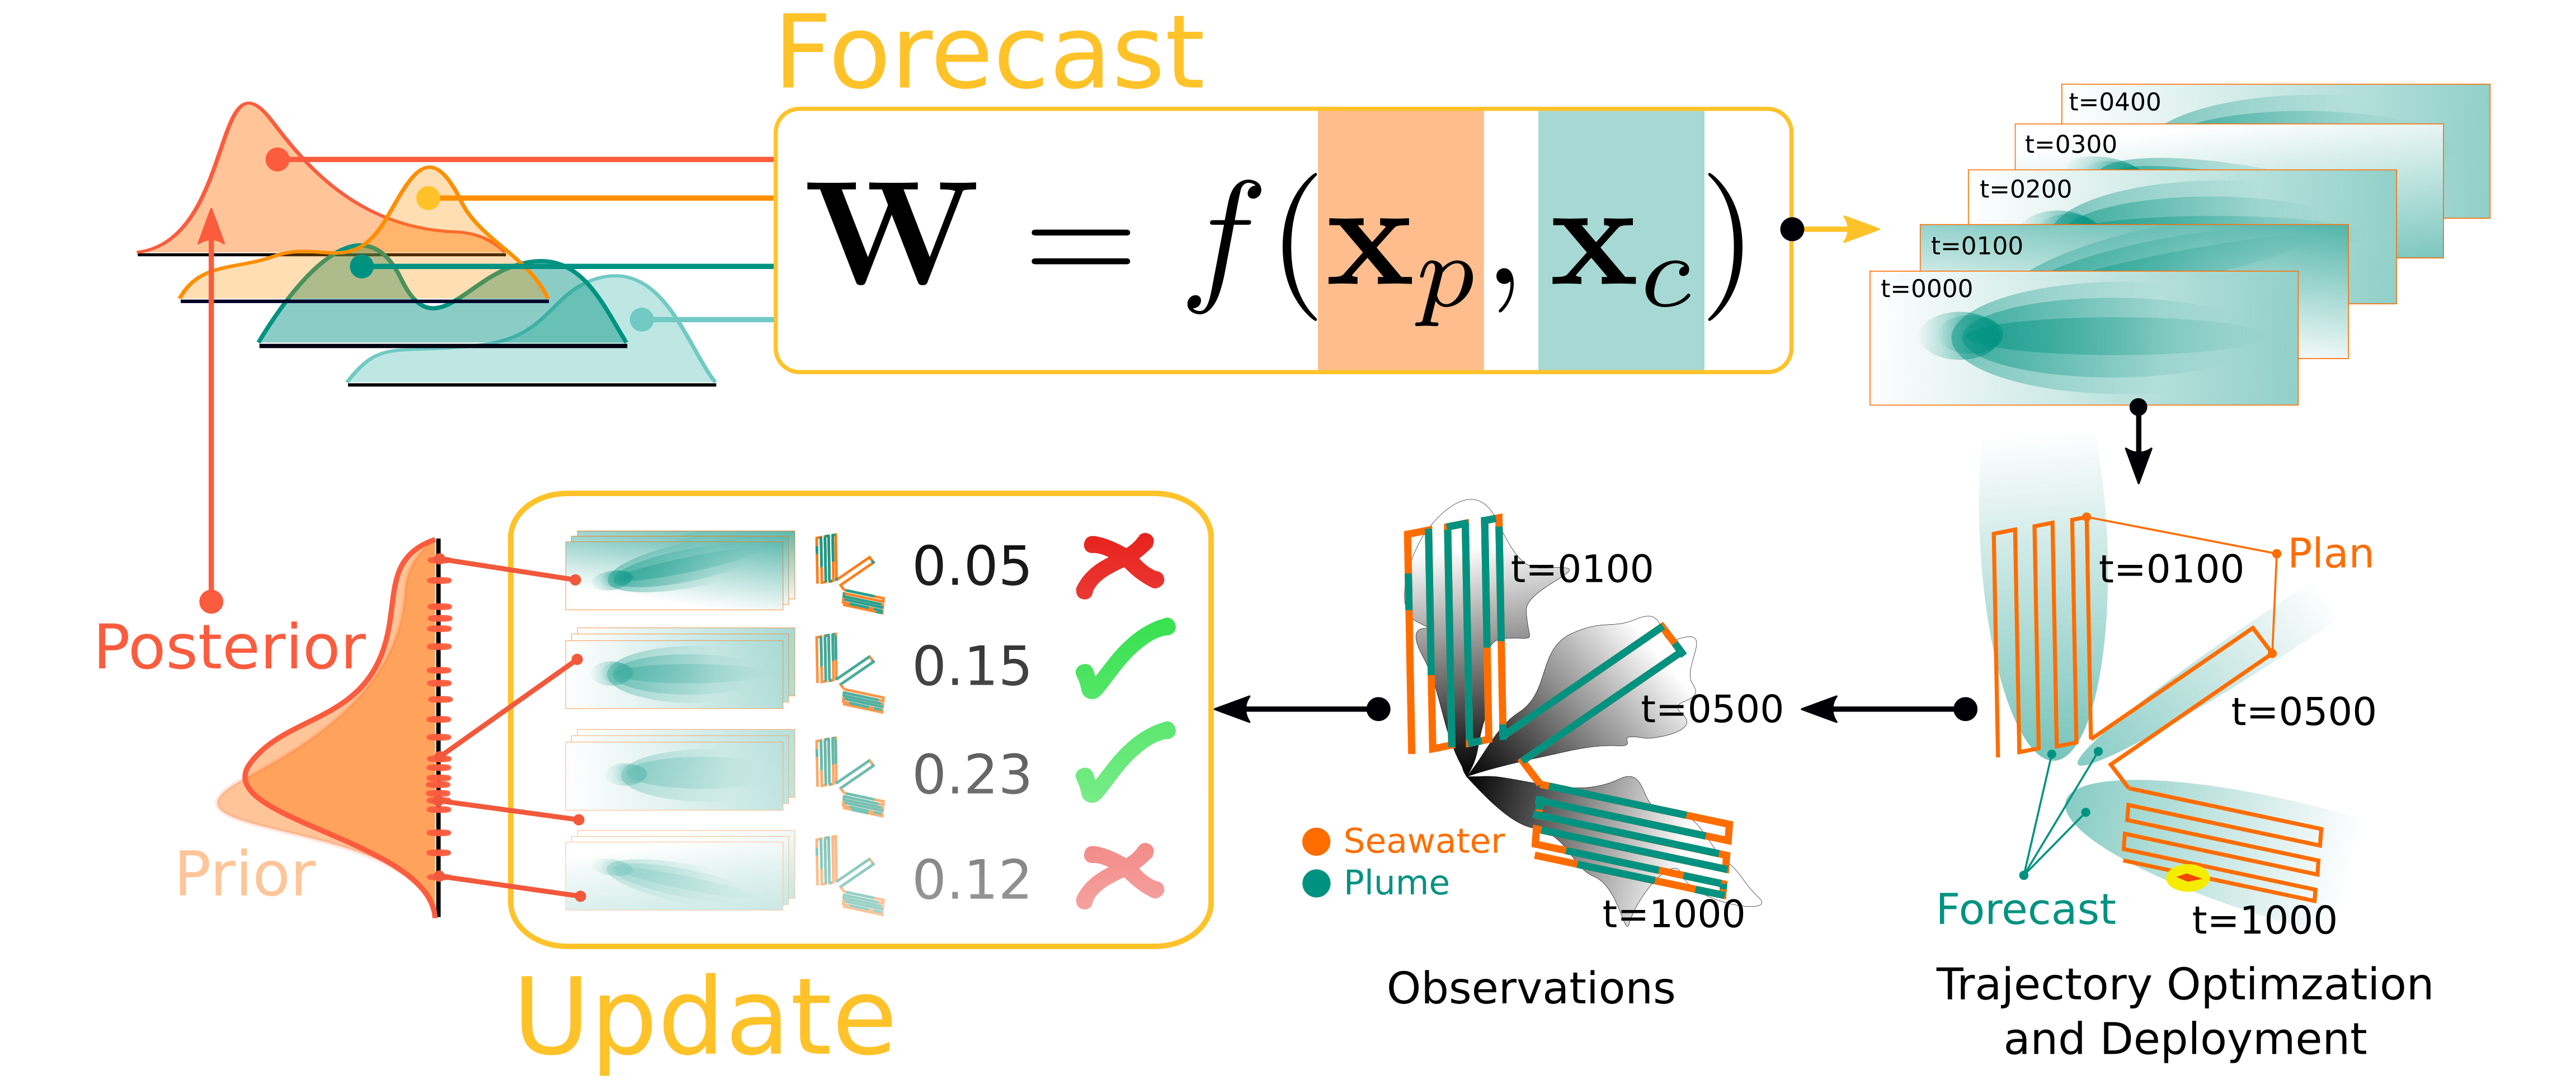
\includegraphics[width=1\columnwidth]{figures/phumes_diagram.png}
    \caption[\PHUMES: \phumes]{\textbf{PHUMES: \phumes}. \PHUMES is a model for forecasting the evolution of a spatiotemporal distribution trained on partial observations. \PHUMES generates forecasts by leveraging an embedded analytical model $f(\cdot, \cdot)$ that approximates the physics-driven evolution of a target distribution. This model is seeded with many samples from distributions placed over initial conditions, physical parameters, or temporal functions (such as $\x_p$ and $\x_c$ here). The composite result of this process is a forecast $\mathbf{W}$ that consists of a mean and variance of phenomenon occupancy in a 3D volume over snapshots of time. This forecast is provided to a trajectory optimizer which sets a deployment trajectory that is executed by a robot. The deployment generates a series of observations, which are then used to update the distributions of the generating distributions via MH-MCMC, which compares the gathered observations with the simulated observations of samples from the generating distributions. The resulting posterior update over the generating distributions is then used for the next planning iteration.}
    \label{fig:phumes}
\end{figure}

\PHUMES consists of two key phases: forecasting (forward simulation) and updating (inverse problem) (\cref{fig:phumes}). In the forecasting step, samples from the distributions of the initial conditions and seawater properties seed the simulator which is solved many times to create a set of plume-envelope samples in the full state space of the target phenomenon (and trajectory optimizer). Time is discretized over domain-specific key points, and any parameters reliant on time are sampled at those discrete points. The set of composite samples at each time is a ``forecast'' that is essentially a series of snapshots of the phenomenon. Precisely, \PHUMES generates a time-indexed $t \in \mathbb{T}$ composite estimate of the distribution of plume fluid in a 3D volume $\overbar{\mathbf{W}}$ by forward simulating time-dependent $M$ samples of the states $x_{p,t}^{(m)} \sim \mathcal{P}(\x_p(t))$ and $x_{c,t}^{(m)} \sim \mathcal{P}(\x_c(t))$ through the plume simulator $f(\cdot, \cdot)$:

\begin{equation}
    \mathbf{W}_t = f(x_{p,t}^{(m)}, x_{c,t}^{(m)}) \hspace{1cm} \forall t \in \mathbb{T}.
\end{equation}

The complete forecast $\mathbf{W}_t$ is the robot's belief $b$, and since it consists of a set of samples, any statistical measure (the maximum \emph{a posteriori} estimator (MAP), maximum likelihood estimator (MLE), median, etc.) can be computed and used downstream by a trajectory optimizer to approximate the reward function $R([\x_p, \x_c, \x_r]^T, a) = \indic{\texttt{in\_plume}(\x_p, \x_c, \x_r, a)} \approx \indic{\texttt{in\_plume}(\Phi(\mathbf{W}), a)}$, where $\Phi(\cdot)$ is some statistical computation. For instance, the variance of the forecast $\mathbf{S}^2_W$ and mean $\overbar{\mathbf{W}}$ can be computed and used within an information-theoretic reward function (e.g., upper confidence bound), as contingent on the design of a downstream planner. 

After the trajectory optimizer yields a plan, \Sentry is deployed within several hours of the plan generation (following a safety check by the engineering team). For a single deployment, upwards of 20,000 observations may be available (each deployment is a minimum of 6 hrs in duration, up to 24 hrs, and sensor measurements are logged at 1 Hz). Using the filter described in \cref{sec:sensor_models}, AUV \Sentry provides observations of binary plume detections. Other sensors of opportunity described in \cref{sec:external_current} provide continuous crossflow magnitude and heading observations. These observations are collated into the sensor model $\Zz$.

At the update step of \PHUMES, the probability distributions over $\x_p$ and $\x_c$ are updated from observations $\Zz$. To find $\mathcal{P}(\x_c|\Zz)$ GP models are trained for crossflow magnitude and heading from external sensor data as referenced in \cref{sec:external_current}. The GP kernel parameters are updated using a maximum-likelihood update following typical procedures \autocite{Rasmussen2004}. For $\mathcal{P}(\x_p | \Zz)$, a random-walk Metropolis-Hastings Markov Chain Monte Carlo (MH-MCMC) method \autocite{metropolis1953equation} is used to perform the update. Simulations of deployments are generated by casting the traversed path over solutions to the numerical model $f(\cdot, \cdot)$ seeded with samples from $\x_p$ and $\x_c$. The output of the simulations is directly compared via a likelihood model with the binary observations of plume waters collected by \Sentry. To handle binary measurements, the Brier score \autocite{brier1950verification} is computed over the set of real observations $\Zz$ and set of predictive probabilities $\rho(\cdot)$ of the corresponding simulated observations: $\frac{1}{|\Zz|}\sum_{i=1}^{|\Zz|} (\Zz^{(i)} - \rho(f(x_p, x_c)^{(i)}))^2$. In practice, the predictive probabilities $\rho(\cdot)$ are set according to an expected false positive rate and false negative rate for instantaneous sensor measurements established in consultation with instrument experts on the science team; they are set to 0.1 and 0.3, respectively. With the likelihood model applied, an acceptance criteria of the likelihood and evaluated priors over samples of $\x_p$ is defined, and samples probabilistically accepted or rejected accordingly. As MH-MCMC inference method is a chaining procedure, each sample of $\x_p$ selected is informed by the last, and the cumulative distribution of all accepted samples is guaranteed to converge to the true underlying distribution for each of the elements in $\x_p$ for long enough chains. The posterior distribution $\mathcal{P}(\x_p | Z)$ is set as the new sampling distribution for the next forecast to be generated.

While formulated here for a single instance of a plume, it would be trivial to extend \PHUMES for inference over or simulation of the generating parameters of multiple co-located vents by jointly updating parameter vectors for each vent. For scalability, choosing a different chaining procedure to accelerate search through a higher dimensional state space at the update step (for instance, Hamiltonian Monte Carlo \autocite{duane1987hybrid}), could be advantageous.


\subsection{Trajectory Optimization with Fixed Patterns}
\label{sec:to}
Given the hydrothermal plume-charting POMDP model introduced in \cref{sec:problem} and the probabilistic plume predictions generated by \PHUMES, how to select trajectories for AUV \Sentry that will effectively map the spatiotemporal dynamics of the evolving plume may be considered. %A specific planning problem is first defined by re-writing the POMDP value function, \cref{eq:value}, in terms of the elements of the hydrothermal POMDP; then, we introduce a sequence of approximations that allow the value function to be feasibly optimized to select high-reward actions.

In each deployment, the planner must select an action in the form of a chained lawnmower trajectory (\cref{fig:traj_opt}). A chained lawnmower is defined by the number, $n \in \Z^+$, of lawnmower trajectories in the chain and the parameters of each individual lawnmower trajectory, $\theta_i \in \Theta$ for $i = 1, \dots, n$. These parameters include the height, width, resolution, origin, and orientation of the pattern and are sufficient to completely specify a lawnmower trajectory. The set $\Theta$ is defined to enforce that the lawnmower trajectories are contained within a pre-defined, rectangular safe region and that each lawnmower obeys a time-based budget constraint. As previously mentioned, this constrained action set is dictated by the operational practices of AUV \Sentry; lawnmower trajectories result largely in \Sentry traveling in straight lines with few, intermittent turns, which is a beneficial paradigm for the navigational sensors used onboard (i.e., acoustic Doppler Velocity Logger (DVL), inertial sensors). Using lawnmower trajectories has the additional benefit of biasing the vehicle to collect spatially diverse datasets that scientists are accustomed to analyzing. 

\begin{figure}[h!]
    \centering
    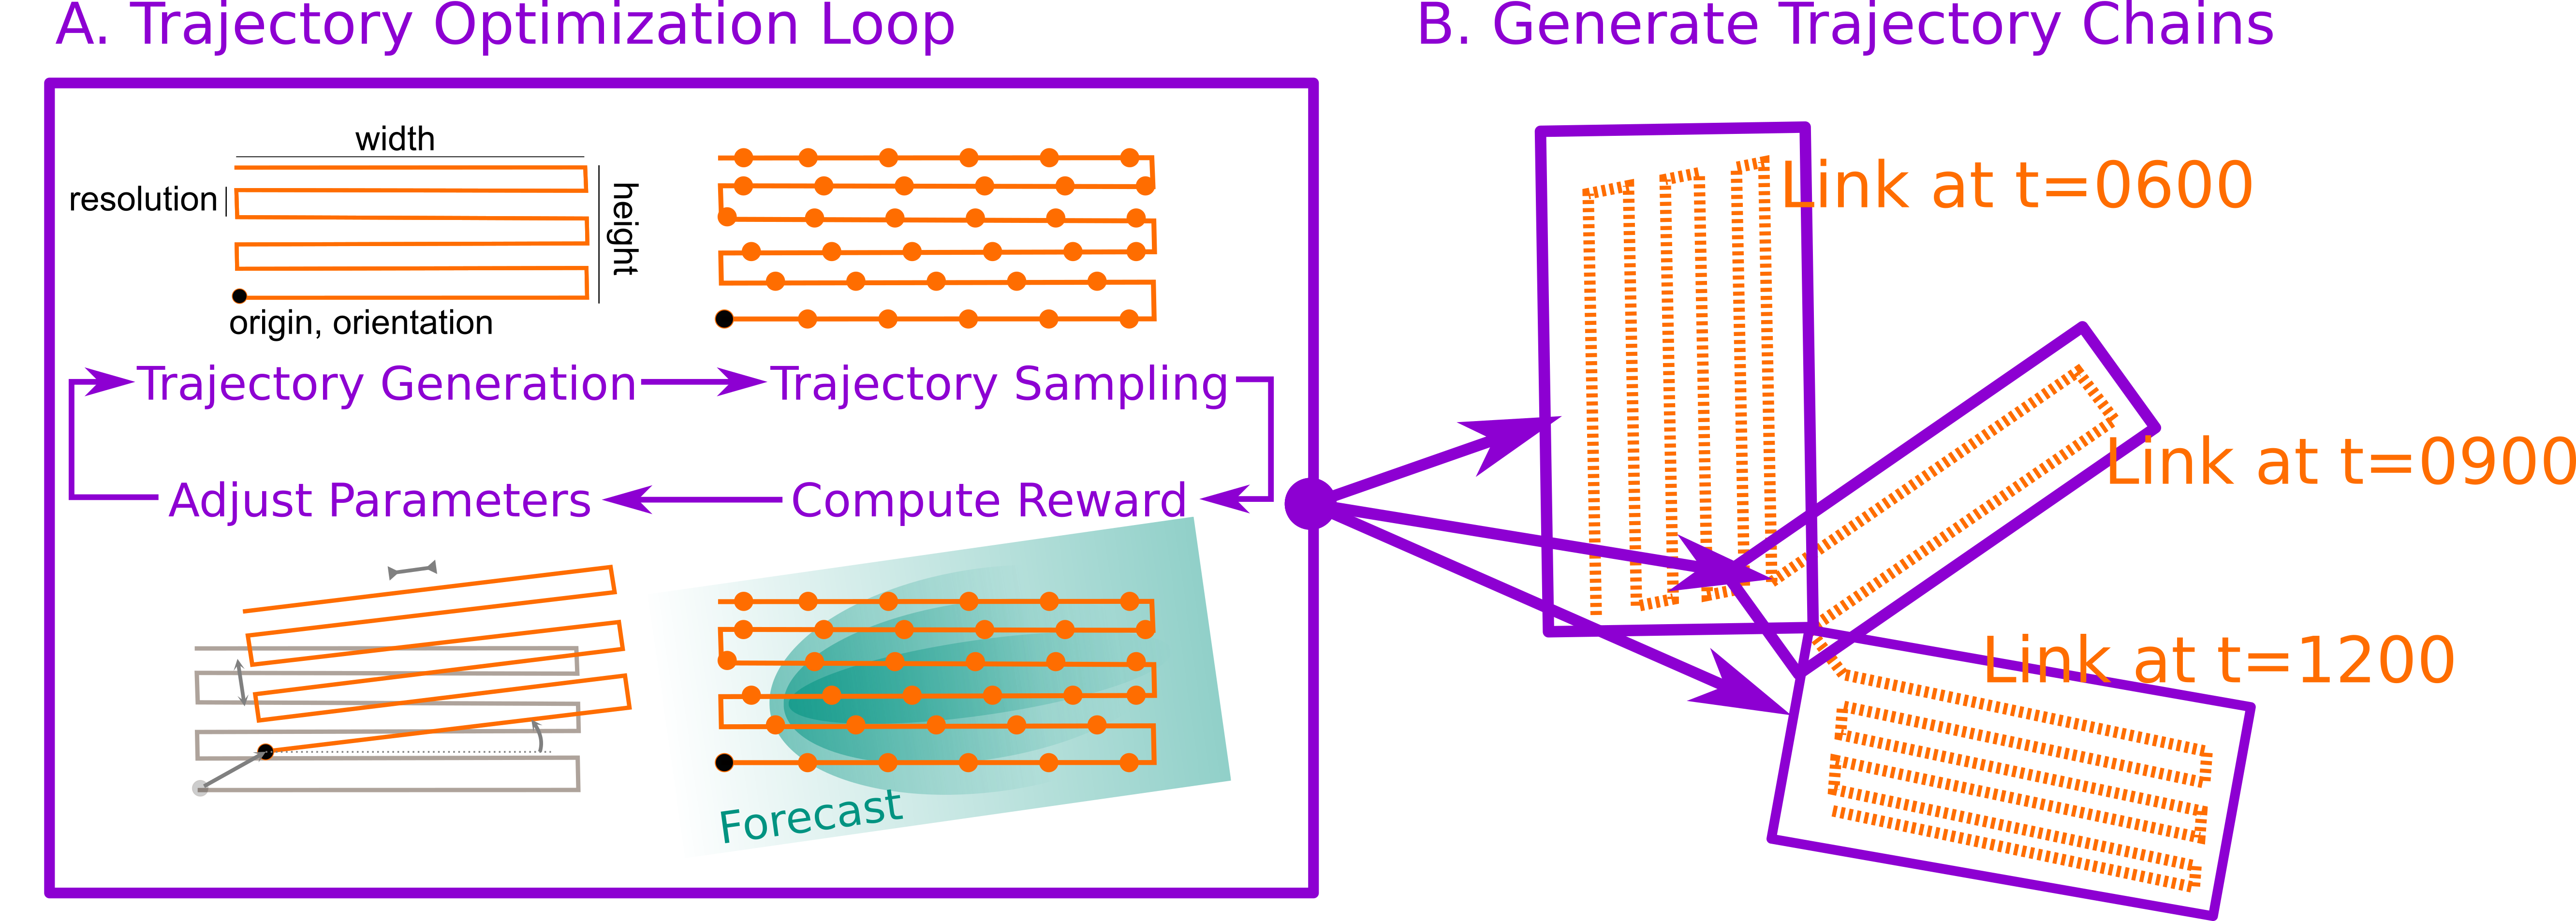
\includegraphics[width=1\columnwidth]{figures/phortex_to.png}
    \caption[Trajectory optimization in \PHORTEX.]{\textbf{Trajectory Optimization in PHORTEX.} The trajectory optimizer leverages the \PHUMES simulator to select high-reward chains of parameterized lawnmower trajectories. (A) The optimization loop for a single lawnmower object, parameterized by height, width, resolution, origin, and orientation. To evaluate the reward of a specific parameter setting, (1) the lawnmower trajectory object is generated using the specified parameters; (2) the trajectory is uniformly sampled along its length to produce a set of sample locations; (3) the reward of those sample locations is computed using the \PHUMES model forecasts of the plume envelope; and (4) the lawnmower parameters are adjusted using gradient-based constrained optimization. (B) This core trajectory optimization loop is used to select parameters for each of a chain of $N$ lawnmowers executed at varying times during the deployment.}
    \label{fig:traj_opt}
\end{figure}

The general POMDP value function defined in \cref{eq:value} is reformulated for the elements of the plume-charting POMDP:
\begin{align}
     V_h^{*}(b) &=  \max_{\{\theta_1, \dots, \theta_n, n \mid \theta_i \in \Theta, n \in \Z^+\}} \mathbb{E}_{[\x_{p}, \x_{c}, \x_{r}]^\top \sim b}[R([\x_{p}, \x_{c}, \x_{r}]^\top, \{\theta_1, \dots, \theta_n\})],
    \label{eq:approx_value}
\end{align}
\noindent for $h \in [0, H-1]$ and where each $\theta_i \in \Theta$ parameterizes one of the lawnmower trajectories in a length-$n$ sequence of chained trajectories, and $b$ is the planner's belief about the state of the plume, currents, and robot. In this equation, the first of two important planning approximations made by \PHORTEX is evident. As mentioned in \cref{sec:problem}, the discount factor $\gamma$ is set to zero, removing the second, recursive portion of the value function. This approximation significantly reduces the complexity of approximating the POMDP value function, allowing each deployment to be optimized myopically. As deployments of AUV \Sentry are intermittent, time constrained, and start/end on a ship at arbitrary coordinates, the sequence of deployments are largely decoupled; decisions made in one deployment have very little impact on the achievable reward of the next.
%Practically, this approximation only slightly compromises planner performance. Deployments of AUV \Sentry are constrained to start and end at the static location of the ship and the duration of each deployment is fixed by the operational constraints of the scientific expedition. This result of these operational constraints is that sequential deployments are largely decoupled: decisions make in a deployment have very little impact on the achievable reward of the next deployment. 

Solving \cref{eq:approx_value} still involves selecting the number of chains $n$ and the joint optimization of all $n$ lawnmower trajectories in the chain. For a standard parameterization of a lawnmower (height, width, resolution, origin, orientation), this results in a challenging high-dimensional, non-convex, constrained optimization problem in which the dimensionality of the optimization problem changes with the number of lawnmowers selected in the chain. In a typical 15-hour deployment of AUV \Sentry that uses $n=15$, one-hour chained lawnmowers, this results in a 90-dimensional, non-convex joint optimization problem, which must then further be optimized over the number of lawnmowers $n$. Optimization is additionally complicated because evaluating the reward function is computationally expensive, requiring \PHUMES to produce a prediction of plume probability for the locations sampled by a given lawnmower, and by a lack of analytical gradients for the reward function with respect to the lawnmower parameters (gradients are instead computed numerically). 

To simplify the planning problem further to address chaining optimization, a second approximation is necessary. If the number of chained lawnmowers is given, i.e., $n=N$, then is it possible to decompose the joint optimization of all chains in a trajectory into $N$-independent optimization problems. This approximation breaks a high-dimensional, joint optimization problem into a sequence of much lower-dimensional optimization problems, and is a reasonable approximation if the travel cost between subsequent lawnmowers is not significant. 

The final \PHORTEX value function, with the two approximations described, is given by the following:
\begin{align}
     V_h^{*}(b) &\approx  \max_{\theta_1 \in \Theta} \dots \max_{\theta_N\in \Theta} \mathbb{E}_{[\x_{p}, \x_{c}, \x_{r}]^\top \sim b}[R([\x_{p}, \x_{c}, \x_{r}]^\top, \{\theta_1, \dots, \theta_N\})],
    \label{eq:approx2_value}
\end{align}
\noindent for $h \in [0, H-1]$.

\cref{eq:approx2_value}, which defines multiple, independent, non-convex, constrained optimization problems, is solved using a trust-constrained method in the \texttt{scipy} optimization library for a fixed number of iterations \autocite{conn2000trust}. To evaluate the reward function $R(\cdot)$, a trajectory sampler operator is defined $\mathbf{G}: \Theta \to \R^{3 \times k}$ that takes a trajectory parameter vector as input and produces a set of locations in $\R^3$ that will be sampled when the robot executes the trajectory, where $k$ is the number of sampled points. In practice, the trajectory sampler $\mathbf{G}$ produces the lawnmower specified by $\theta$ and then sub-samples uniformly along its length with a fixed spacing. These sample points can then be compared with the plume forecast $\mathbf{W}$ produced by \PHUMES to count the number of sample points that are contained within the inferred plume.


\section{Simulation Experiments}
\label{sec:experiments}
The performance of \PHORTEX is investigated in a simulated environment designed to replicate the field deployment closely. In the simulation, a point robot is tasked with collecting spatially and temporal diverse samples of an advecting plume. Each simulation is a three-dive series in which \PHORTEX starts with an uninformative prior over $\x_p$ and executes an initial naive survey (as would occur in a realistic field scenario), then iteratively updates \PHUMES with collected observations and uses the the trajectory optimizer discussed in \cref{sec:to} to perform two more dives. Ten three-dive simulations for each sampling/planning altitude of \SI{100}{\meter} and \SI{150}{\meter} are performed in the same environment. Each single dive in the three-dive sequence is designed to be 12 hrs of simulated time, on a scale similar to the field deployment missions (over 50 acres, or \SI{0.25}{\kilo\meter\squared}). 

In the simulator, the underlying analytical model in \PHUMES is used to generate a ground-truth environment that closely matches the conditions of a single real-world vent using available data. The simulated environment has vent conditions of \SI{300}{\celsius} temperature of water at the vent opening, 34.608 PSU salinity of water at the vent opening, \SI{0.8}{\meter\squared} orifice area of the vent, and \SI{0.6}{\meter\per\second} initial fluid velocity at the vent opening. The simulated environment sets the mixing coefficients to 0.15 and 0.2 for horizontal and vertical mixing, respectively. The current function sweeps a generated plume from due North to due East over the course of 12 hours of simulation time, and the magnitude cyclically varies with a beginning and end point of \SI{0.11}{\meter\per\second} and minimum at \SI{0.04}{\meter\per\second}. The generating snapshots of the true environment are provided in \cref{fig:sim_env}.

\begin{sidewaysfigure}
    \centering
    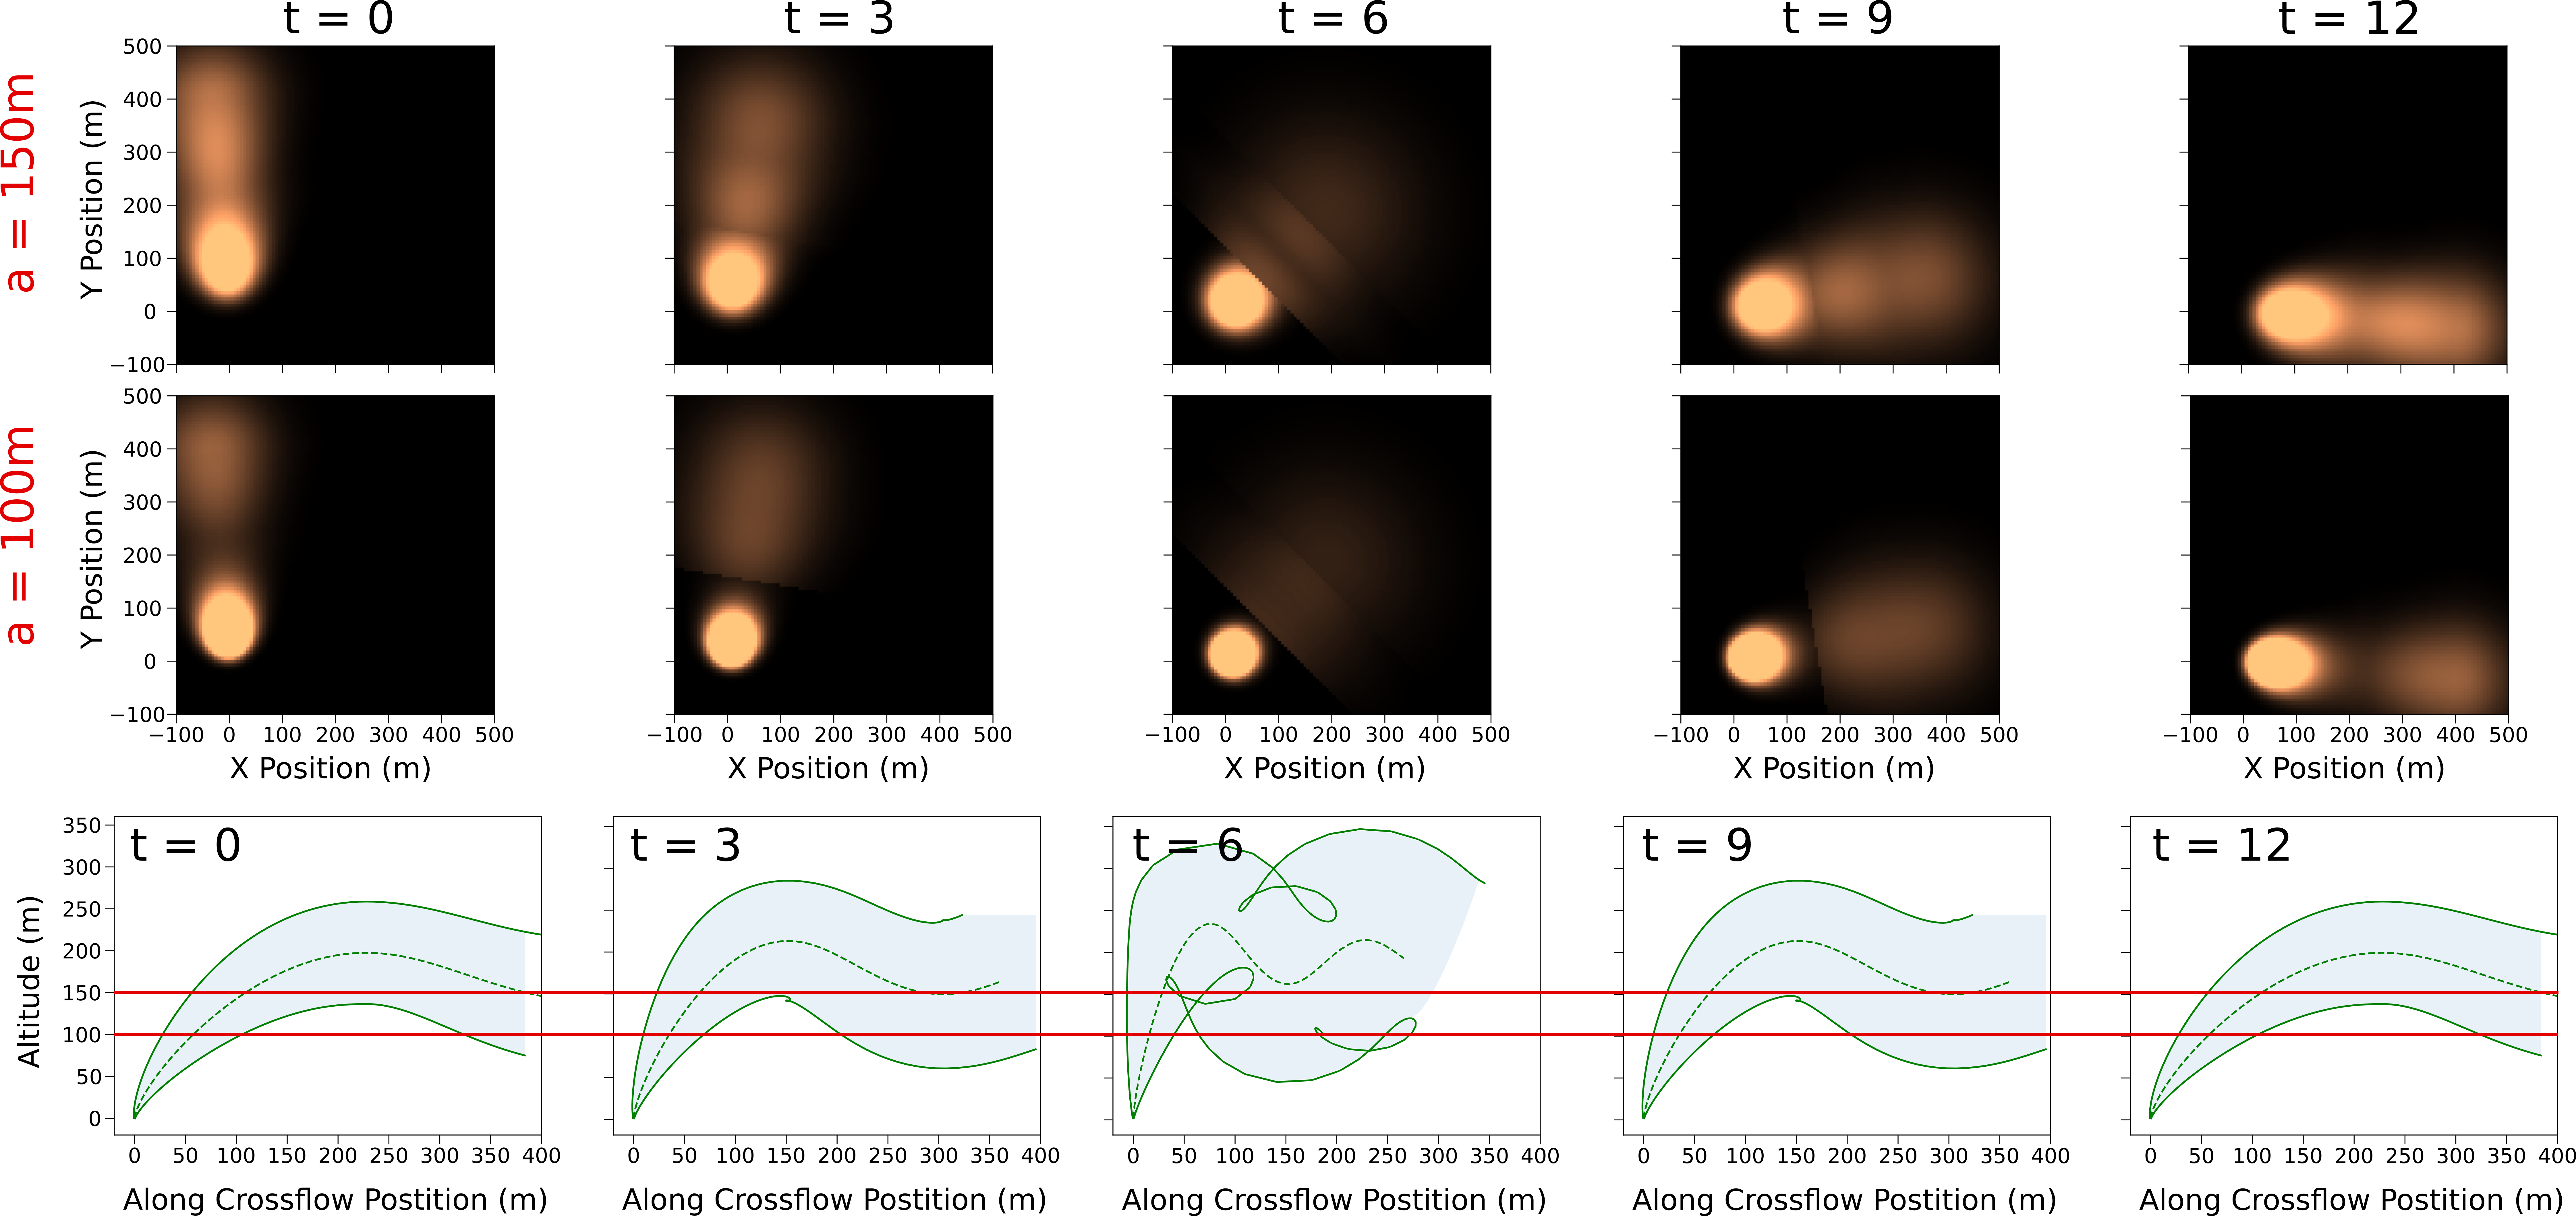
\includegraphics[width=1\columnwidth]{figures/sim_env.png}
    \caption[Simulated field trial environment.]{\textbf{Simulated field trial environment.} Generated environment for simulation trials at different snapshots of time (in hours) for altitudes of \SI{100}{\meter} and \SI{150}{\meter}. As the current magnitude and heading changes, the plume expression changes shape and location over 12 hours. Plume intensity is shown in orange in the top plots. The bottom plots show a vertical cross-section of the plume envelope, along the crossflow direction, at different points in the tidal cycle, with the \SI{100}{\meter} and \SI{150}{\meter} horizontal planes marked.}
    \label{fig:sim_env}
\end{sidewaysfigure}

In these experiments, the \PHUMES model must estimate the vent area, vent fluid velocity, and both mixing coefficients from plume observation in the water column, starting with uninformative priors over each of these targets. A noisy current magnitude and heading function is provided to \PHUMES for use in the forecasting and updating step, as would typically be available from sensors of opportunity in the field. For the \PHUMES update, 150 samples from an MH-MCMC chain are used to approximate the posterior distributions over the inference targets (this excludes an initial 50 samples of burn-in). In the first simulated dive, the robot executes a best-case uninformed lawnmower trajectory, placed to intersect the sweeping movement of the current. This trajectory is \SI{15}{\meter} in resolution, and covers a \SI{500}{\meter} by \SI{500}{\meter} area, with no rotation. For the second and third dives, trajectories are optimized using \PHORTEX for the 12-hour mission and consist of four, 3-hour long chained lawnmowers\footnote{Chain-lengths were dictated by computational constraints placed on the framework to mimic realistic field scenarios, in which only a few hours may be available for plan creation. For more detail on the chaining performance of \PHUMES, see \cref{app:phortex}.}. Each lawnmower in the chain has a fixed resolution of \SI{10}{\meter}, and the height, width, origin, and orientation of each lawnmower are optimized to collect the most reward based on a plume forecast using the maximum \emph{a posteriori} (MAP) sample returned by the \PHUMES model for the four inference targets. The robot travels at approximately \SI{0.5}{\meter\per\second}, collecting binary observations every meter that is traveled.

\subsection{Evaluation Metrics}
\label{sec:eval_metrics}
The scientific objective of \Sentry in the field trial is to collect observations of a deep-sea hydrothermal plume that have broad coverage in time and space, and thus are useful downstream for characterizing the space-time dynamics of the plume and other related phenomena (i.e., chemical flux, consumption). To evaluate the performance of \PHORTEX for deep-sea plume charting in both simulation and field trials, three key metrics that measure how well \Sentry collects such samples are:
\begin{itemize}
    \item \textbf{Proportion of positive plume observations:} the number of observations collected in a dive that are classified as in-plume by the binary sensor model (\cref{sec:sensor_models}). This metric captures how effectively the robot targeted the plume during a deployment.
    \item \textbf{Spatial utilization:} the most distal plume detection and the ratio between the most distal plume detection and the longest distance that the robot traveled from the plume source. This metric captures the spatial coverage of the plume achieved by the robot and the spatial efficiency of the deployment. For example, if detections were made up to \SI{300}{\meter} away from the vent, but the robot traveled up to \SI{1}{\km} away, then the survey spent too much time outside of the detectable plume region and would not be as effective as a survey that only traveled \SI{200}{\meter} away but stayed well within the detectable plume range. 
    \item \textbf{Temporal utilization:} the proportion of hours in the dive with at least 10\% or more plume detections. This metric quantifies how effective the robot was at \emph{staying in} or \emph{revisiting} the plume over time. Given the long duration of these missions, it is important to use the entire mission window for the task at hand; moreover temporally diverse observations are of scientific interest.
\end{itemize}


% Quality for this task is defined as collecting a high-proportion of in-plume samples over the course of a dive, revisiting a plume over the course of a dive, and collecting in-plume samples as far from the vent as the robot drives. 
\section{\PHORTEX Performance}
\label{sec:phortex_perform}
\cref{fig:sim_traj_example} shows example planned trajectories and \cref{fig:sim_traj_perform} shows the distribution of each of the metrics of interest presented in \cref{sec:eval_metrics}---proportion in plume, spatial utilization, temporal utilization---for the three dives at each altitude tested in the simulated trials. These results demonstrate that the \PHORTEX optimized trajectories significantly outperform the uninformed baseline, collecting over twice the proportion of samples in-plume, at least doubling the number of hours that the robot spends in a plume, and improving spatial utilization to nearly 100\% from 60-70\%. For analysis of the convergence characteristics of the optimizer, see \cref{app:phortex}. 

\begin{sidewaysfigure}
    \centering
    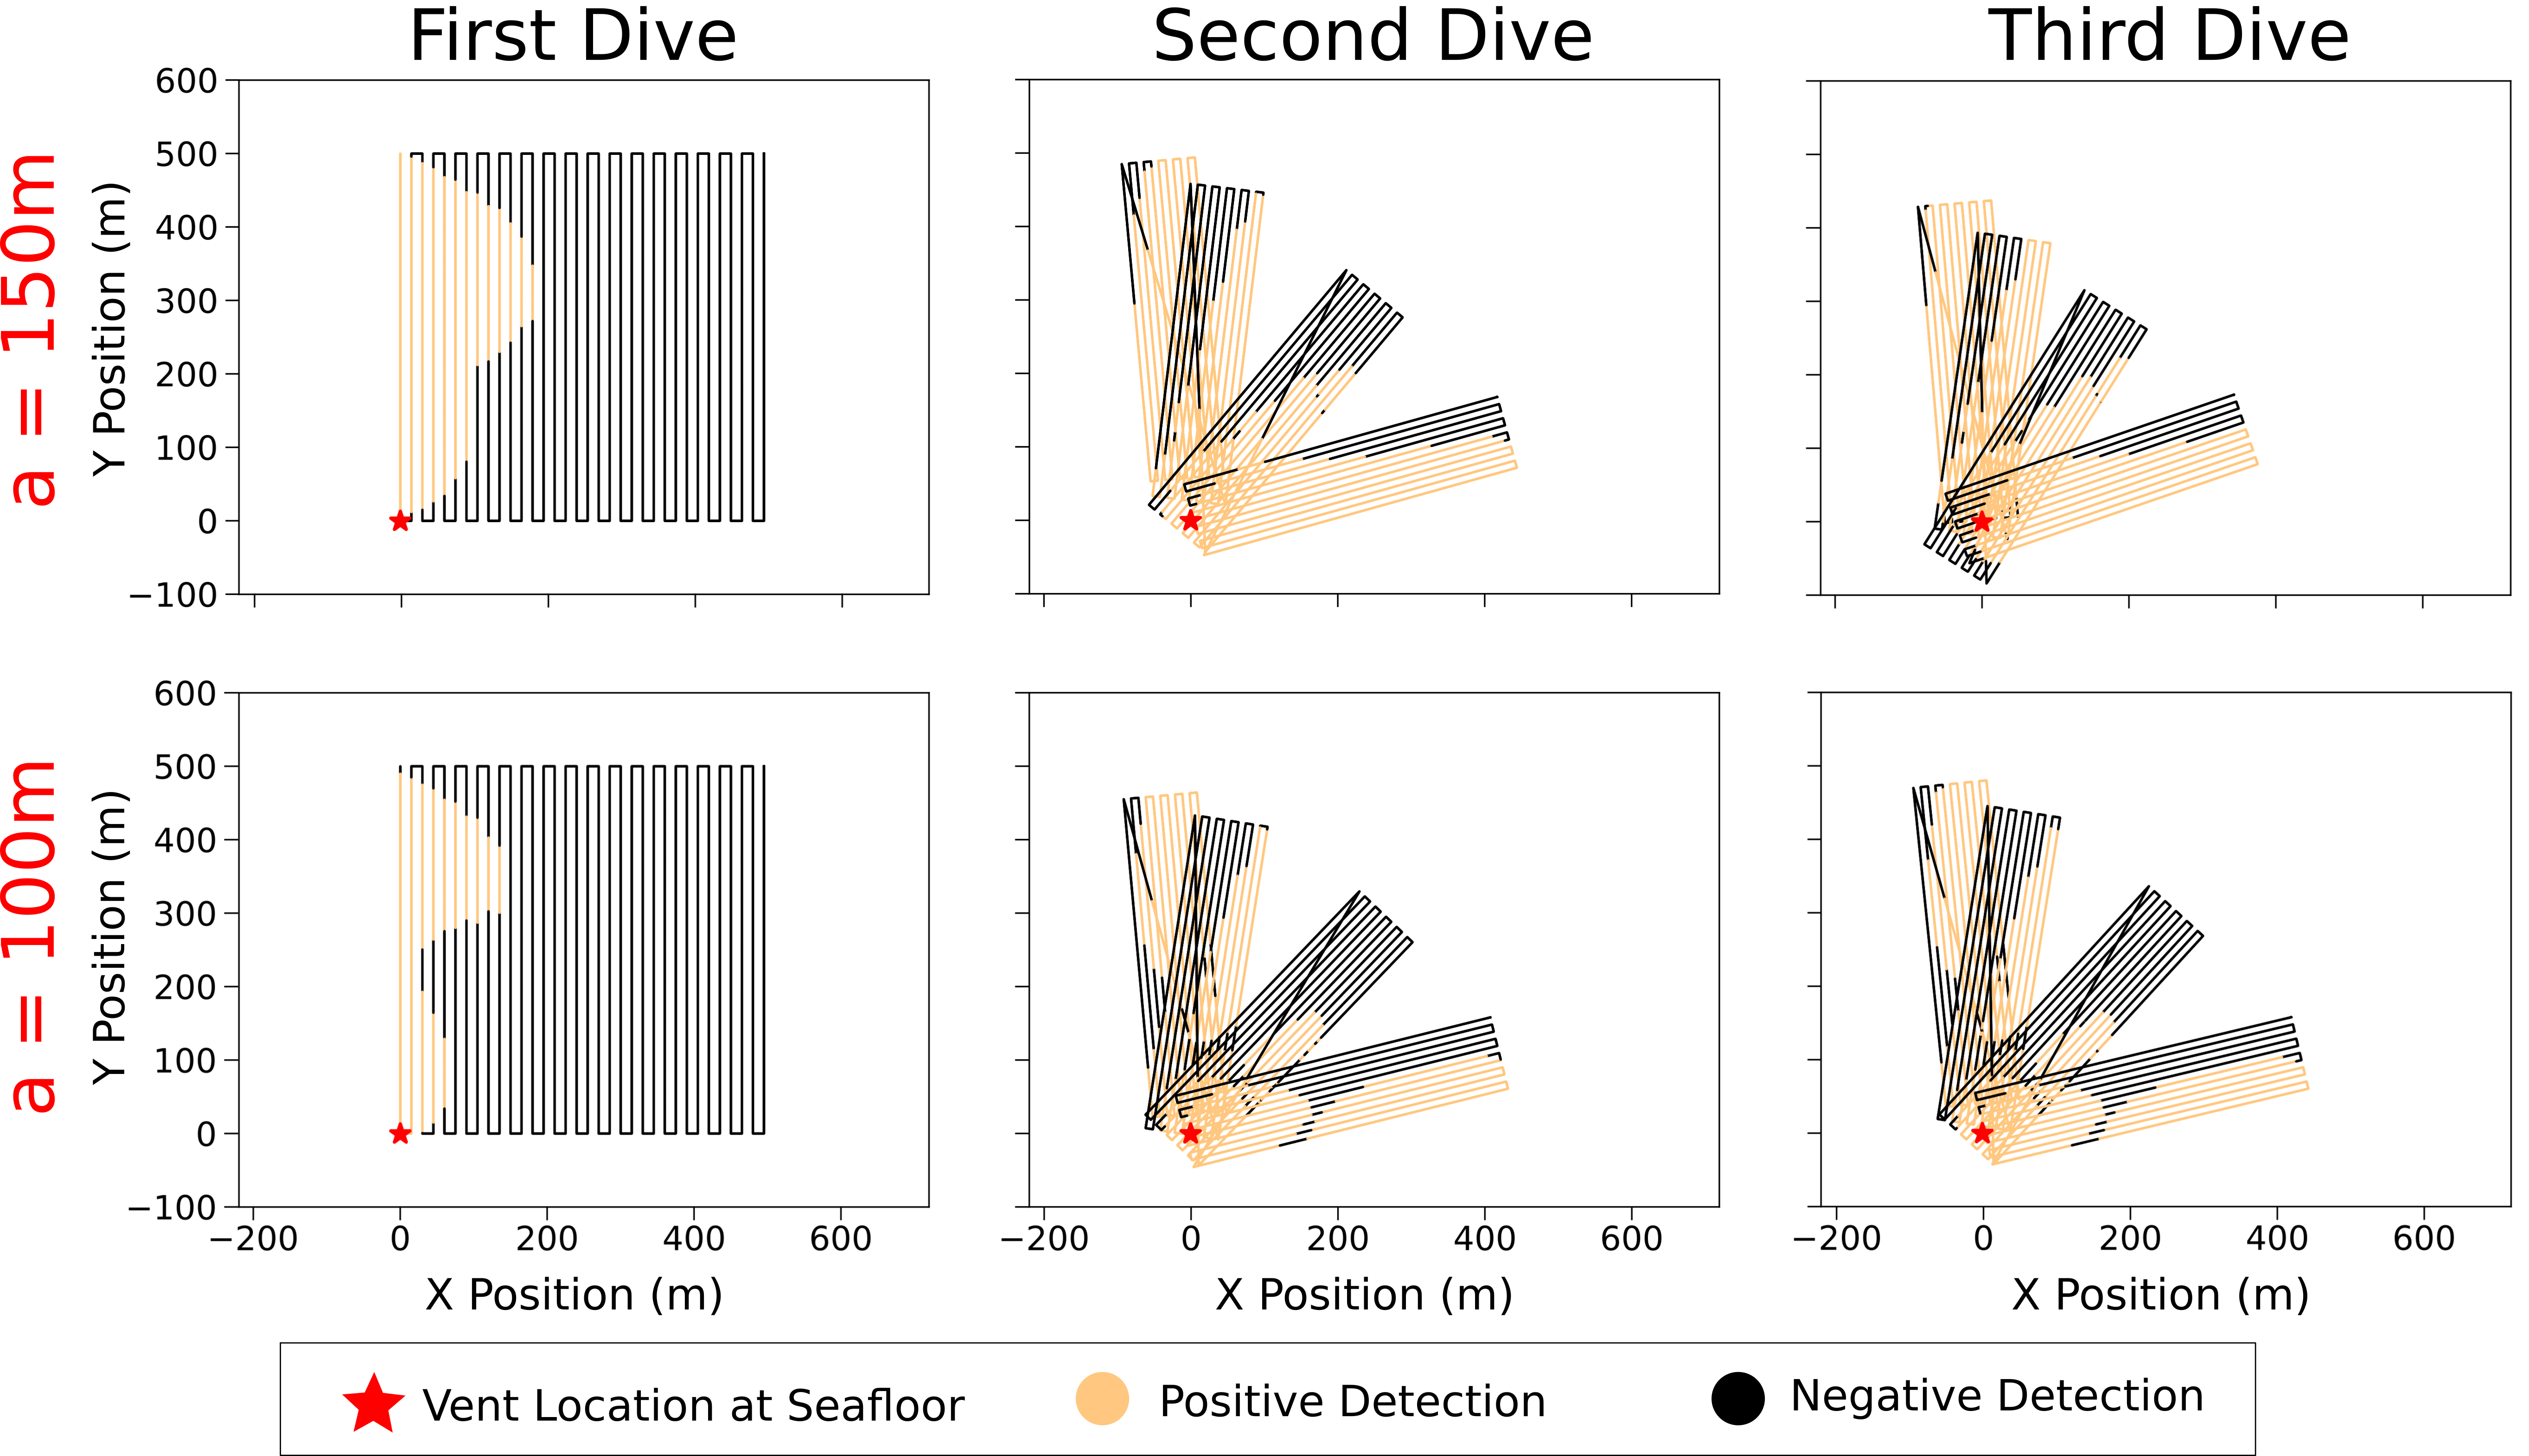
\includegraphics[width=1\columnwidth]{figures/sim_traj.png}
    \caption[Naive and \PHORTEX-design trajectories.]{\textbf{Naive and PHORTEX-designed trajectories.} Trajectory examples for altitudes of \SI{100}{\meter} and \SI{150}{\meter}. The first dive is always a naive lawnmower; the second and third dive are \PHORTEX designed trajectories. \PHUMES is incrementally trained after each dive on the binary plume detections shown in this plot, which are sampled every meter traveled along the trajectory.}
    \label{fig:sim_traj_example}
\end{sidewaysfigure}

\begin{figure}[h!]
    \centering
    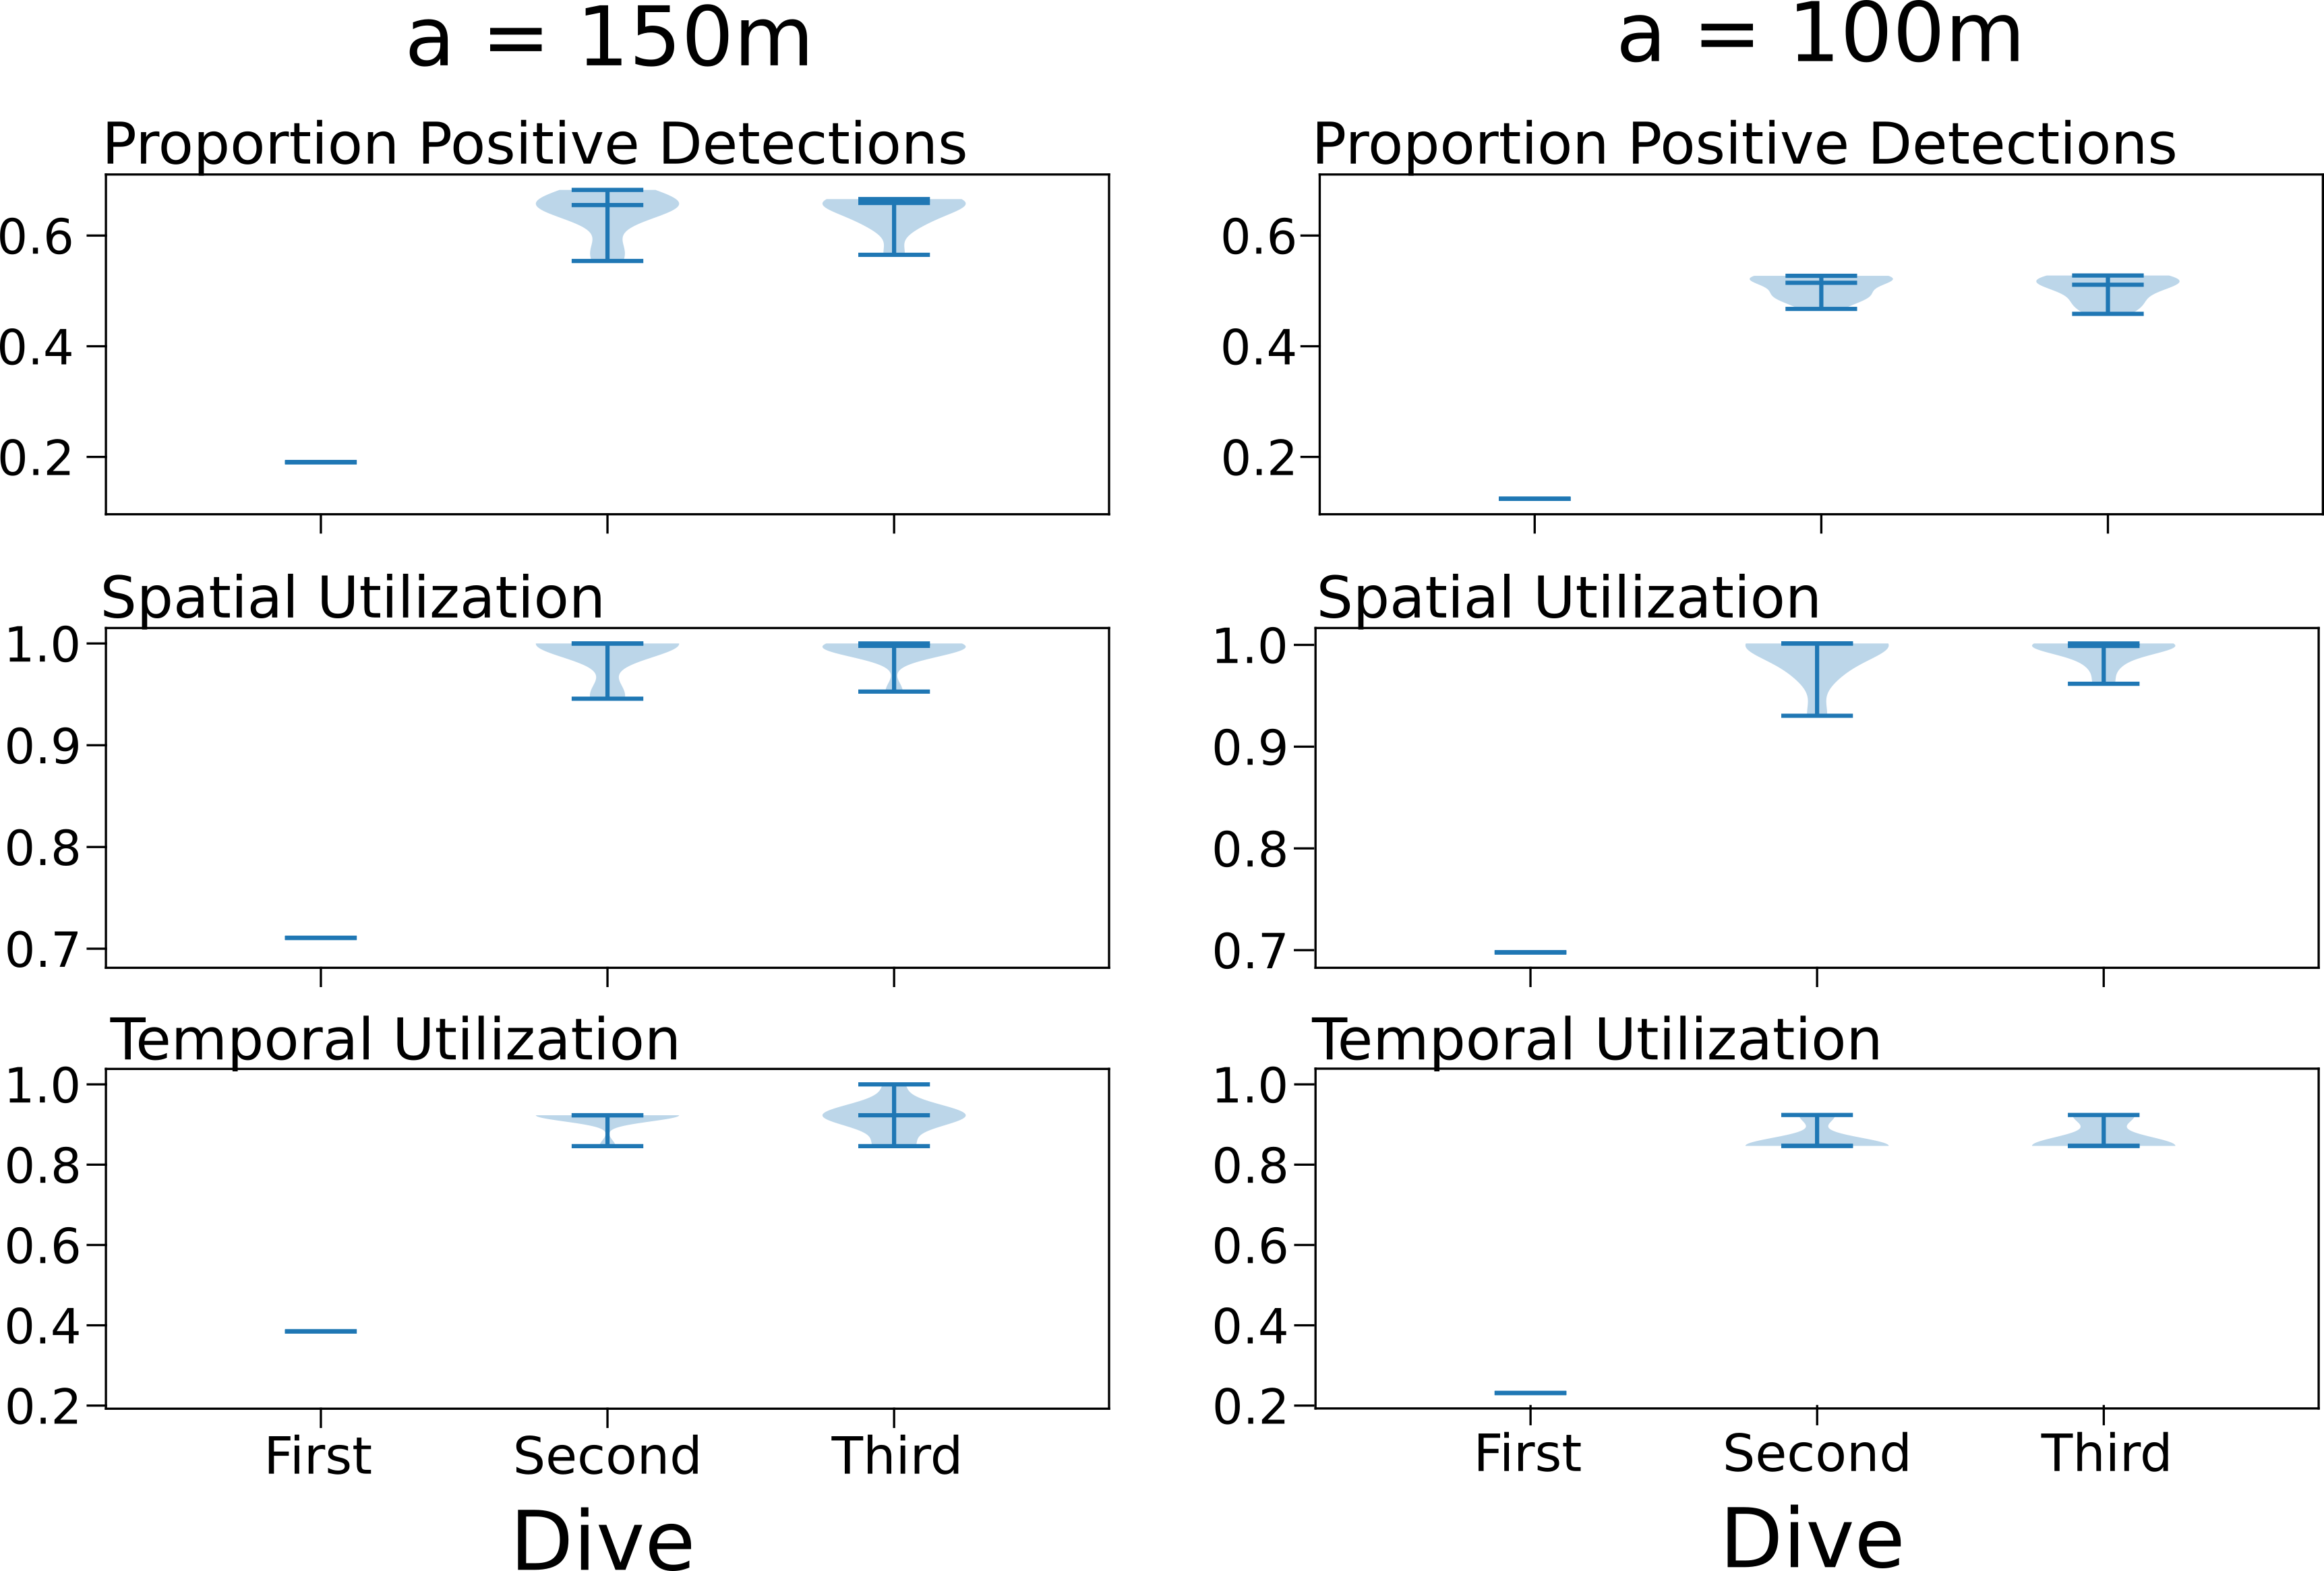
\includegraphics[width=1\columnwidth]{figures/sim_traj_performance.png}
    \caption[Evaluation of the \PHORTEX trajectories.]{\textbf{Evaluation of the PHORTEX trajectories.} The three-dive sequence, consisting of a naive lawnmower followed by two rounds of \PHUMES model training and \PHORTEX trajectory optimization, are evaluated for proportion of positive plume detections, spatial utilization, and temporal utilization (\cref{sec:eval_metrics}). Note that the y-axis for each plot is in the units of the subtitle labels. The \PHORTEX-designed dives show a clear improvement in all three metrics, gathering more spatially and temporally diverse observations of the dynamic hydrothermal plume. Iterative rounds of \PHORTEX model-training and trajectory optimization continue to collect a high proportion of scientifically valuable observations.}
    \label{fig:sim_traj_perform}
\end{figure}


\section{\PHUMES Model Validation}
\label{sec:phumes_perform}
The performance of \PHORTEX stays consistently high in the second and third dives, suggesting that \PHUMES quickly learns a sufficient model for planning from the small number of samples collected by the naive trajectories. To further understand the model learned by \PHUMES, qualitatively inspection of the models learned by \PHUMES in two exemplar trials are inspected with data collected at \SI{100}{\meter} and \SI{150}{\meter} altitude during the initial naive survey of the first dive, as presented in \cref{fig:sim_model}. In the naive survey, less than 20\% of all detections are positive detections, and all detections only occur in the first 3 hours of the 12 hour mission. At an altitude of \SI{100}{\meter}, the robot essentially ``skims'' the bottom of the neutrally-buoyant plume; at \SI{150}{\meter}, the robot is consistently within the range of the neutrally-buoyant plume. Despite these altitude differences, models learned in this example show remarkably similar characteristics---a predicted centerline no more than \SI{25}{\meter} off from the true environment's centerline, and a width that nearly completely envelopes the true plume distribution, which is promising for the context of planning missions. This is in contrast with an illustrative sample from the uninformative prior, which can arbitrarily produce plume structures that are significantly different in form from the true generating environment. It is also worth noting that positive detections of the plume were made only in the first 3 hours of the 12 hour simulated dive; despite this temporal clustering of detections, the predictive quality of the model forecasts to an unseen time ($t$=9hrs) remains high. This largely demonstrates the advantage of using an embedded dynamics model to generate predictions of the state space to unseen times.

\begin{sidewaysfigure}
    \centering
    \includegraphics[width=\columnwidth]{figures/sim_mod.png}
    \caption[Illustration of model learning.]{\textbf{Illustration of model learning.} Snapshots of the true generating environment are compared with an arbitrary sample from the prior distribution over \PHUMES parameters and the learned models from data collected by naive lawnmowers in both \SI{100}{\meter} and \SI{150}{\meter} simulation trials. In these two exemplar experiments, model learning performance is comparable between the \PHUMES models trained on data from different altitudes. The learned model, in comparison to the baseline sample, demonstrates a lower neutrally buoyant stem height, and is wider, and better explaining the data collected at the two sampling heights. Snapshots at different times show that the learned parameters robustly predict future shapes of the plume, even when trained on partial data available from the naive lawnmowers.}
    \label{fig:sim_model}
\end{sidewaysfigure}

To quantify the performance of the plume forecast generated by the MAP parameter sample after each trial, the intersection over area (IoA) and intersection over union (IoU) between the true environment and each of the learned models after the naive and first \PHORTEX designed simulated dives are computed (\cref{fig:sim_phumes_perform}). A set of 10 parameter samples from the uninformative priors over the inference targets are used to generate a performance distribution representative of the initialized model, to show the breadth of forecast quality before any training. IoA (or recall) provides a number from 0-1 that expresses how many samples predicted by the learned model to be in the plume are in the plume of the true generating environment. This number does not penalize false positives in the model: a value of 1 implies that all points in the model are contained by the environment, and a 0 implies that there are no points contained in the true environment. IoU (or precision) also provides a number from 0-1 that now penalizes false positives: a value of 1 implies perfect alignment between the model and environment, and a 0 implies no alignment. The comparison of these numbers helps to contextualize the performance of model learning. 

In \cref{fig:sim_phumes_perform}, the learned models are shown to have a narrower performance window than the baseline samples, and that they generally exhibit very high IoA (up to 1), and a higher IoU (up to 0.9) than the baseline models (up to 0.75). With a high IoA, there is confidence that the learned models are placing predictions in areas where the true plume is present, and with a higher IoU, there is confidence that the structure of the predicted plume regions aligns well with the true environment. Taken together, a very high IoA with medium to high IoU suggest that trajectories planned with the \PHORTEX-trained models are very likely to plan for and successfully execute intersections with the targeted plumes, which is advantageous for the scientific task. There is no degradation of performance with different observations available between dives, suggesting that from very little data (a single naive dive), an immediately useful model can be trained.

\begin{figure}[h!]
    \centering
    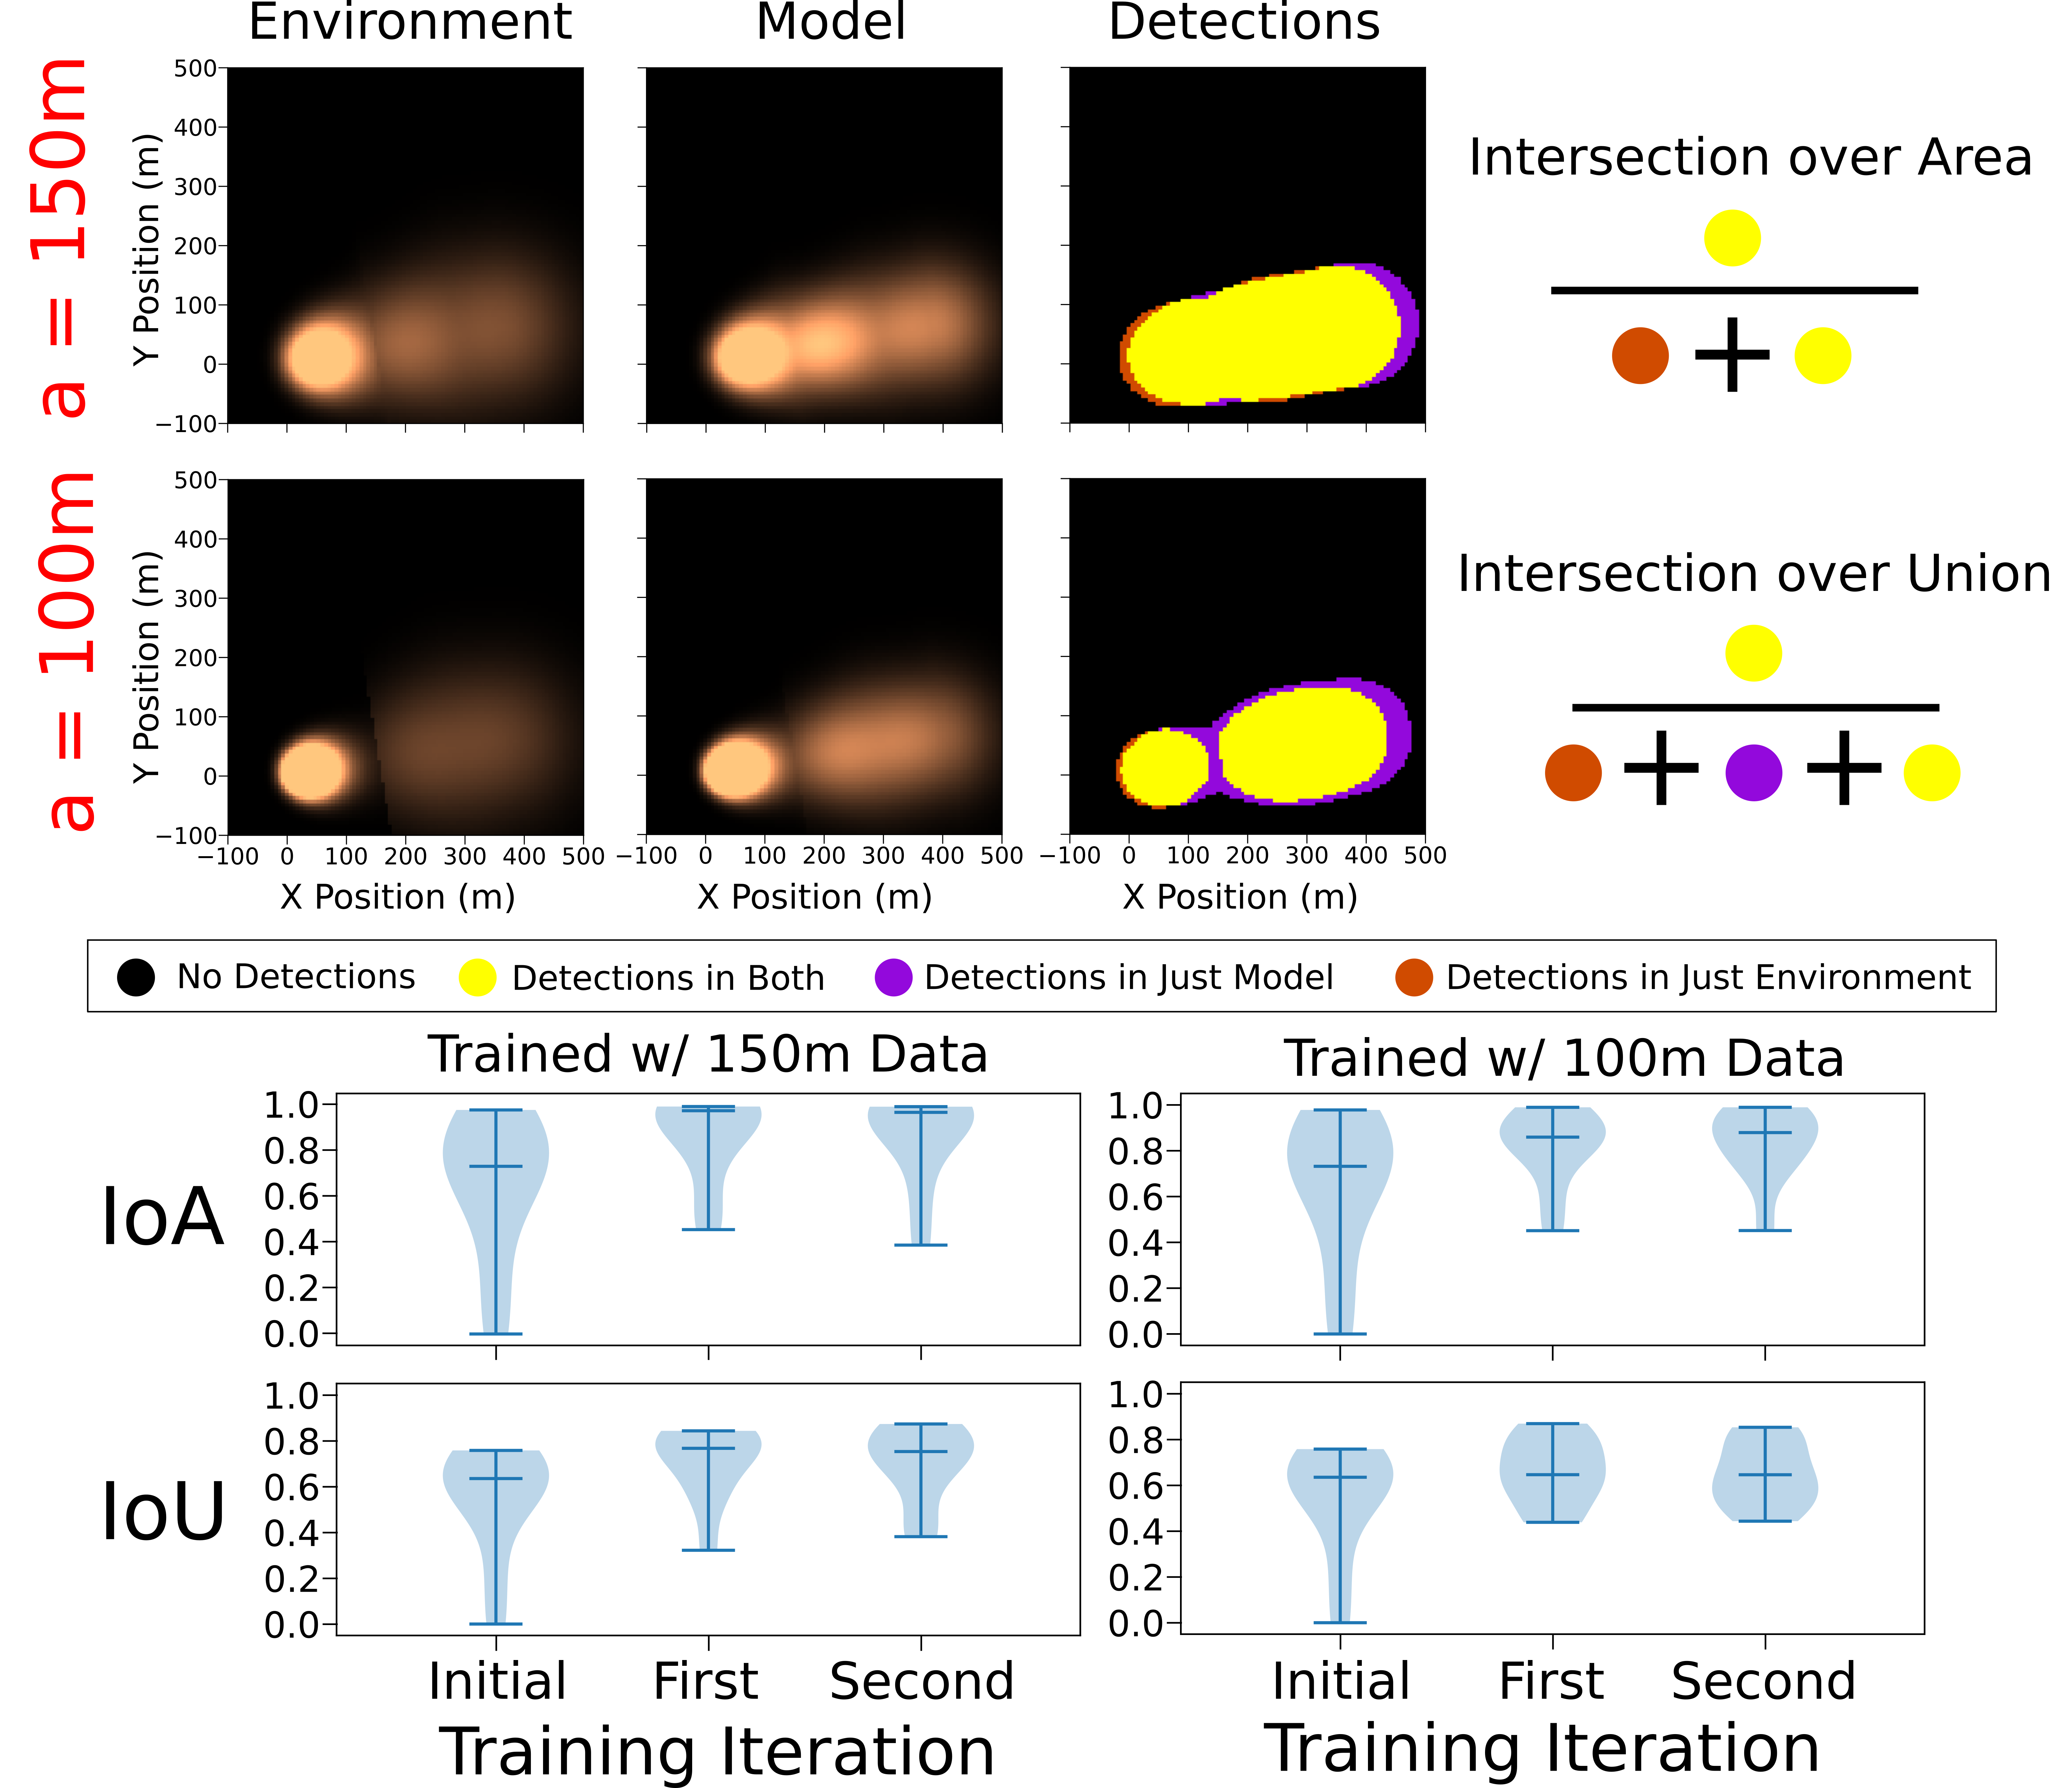
\includegraphics[width=0.9\columnwidth]{figures/sim_mod_performance.png}
    \caption[Intersection over Area and Intersection over Union of trained models.]{\textbf{Intersection over Area (IoA) and Intersection over Union (IoU) of trained models.} For each of trials trained from data at \SI{100}{\meter} and \SI{150}{\meter} altitudes, the average IoA and IoU are computed (using the method illustrated at the top) for a set of initial model samples (Initial), \PHUMES trained on the naive dive (First), and \PHUMES trained on the follow-up \PHORTEX-designed dive (Second) in simulation. IoA and IoU are both measures from 0-1. IoA does not penalize false positives; a 1 implies that all points predicted to be in the plume in the model are plume samples in the true generating environment. IoU penalizes false positives; a 1 implies perfect agreement between the model and true generating environment. In general, each of the iterative trained dives maintains similar performance; with high IoA and medium-to-high IoU that is consistently higher than initialized samples. Trials trained on data from \SI{150}{\meter} tend to have more performant model estimates (IoA near 1, IoU skewed above 0.8) compared to those trials trained on data from \SI{100}{\meter}.}
    \label{fig:sim_phumes_perform}
\end{figure}

Notably, there is a distinct difference in the distribution shapes of IoA and IoU between the altitudes across these trials. In particular, training from samples at \SI{150}{\meter} appears to be more consistently highly performant (IoA mode is at or near 1; IoU distributions skew towards 0.8) than at the lower altitude, which has a more distributed performance characteristic (with IoA skewed around 0.8, and IoU centered just above 0.6). This has interesting implications for choosing deployment altitudes in practical missions, within the constraints of robot abilities (for instance, AUV \Sentry cannot swim over a certain altitude and maintain good localization, thus constraining what parts of a plume may be accessible in field deployments). This sets up a direction for future work to characterize the informativeness of different plume regions for model recovery in scientific settings.


\section{Discussion and Future Work}
\label{sec:phortex_future}
Through this simulation work, \PHORTEX is shown to be an autonomy system that can effectively leverage scientific knowledge to enable a deployment-by-deployment mission to chart deep sea hydrothermal plumes. Quantitative gains over typical exploration strategies in terms of number of total in-plume samples, as well as the spatiotemporal diversity of those samples, lends confidence in the ability for this framework to perform in real field settings. As technological advances in robot platforms increase for scientific contexts, advancing \PHORTEX for online settings and adapting multiagent strategies for deep-sea research are attractive next steps. For \PHUMES, improving upon the temporal expressivity of the model presented in this chapter, investigating pre-training opportunities with sophisticated simulators, and adapting state-of-the-art scientific machine learning techniques for a decision-making context, are areas of direct improvement that can be studied. The following sections discuss some of the key challenges in deploying \PHORTEX for hydrothermal plume charting, each of which may be avenues for future work.

\subsection{Temporal Resolution in \PHUMES Forecasts}
The \PHUMES forecast provides a sequence of time-averaged plume ``snapshots'' over which trajectories for a given dive can be planned. By virtue of using the analytical model presented in \cref{sec:phumes}, generating a series of snapshots requires discretizing over time in order to sample a crossflow magnitude and heading, with which the global coordinates of a plume can be computed. This strategy does not capture the effects of advection and mixing on pre-existing (i.e., persistent) plume fluids; the snapshot from $t=0$ does not influence the snapshot of $t=1$ because the persistence of plume fluids generated at $t=0$ are not modeled directly. For the purposes of plume charting in the neutrally-buoyant layer, it could be advantageous to have a more sophisticated model of plume-fluid persistence and/or finer-scale temporal resolution in order to better constrain the spatiotemporal coordinates of a particular observation. For this sophistication to be added, two key innovations would be necessary: a suitable analytical model and a suitable observation scheme.

In settings in which modeling fluid persistence may be useful, a simple advection-diffusion model could be applied on-top of the analytical model used in this work to advect neutrally-buoyant fluids between time discretized snapshots. This would be a simple extension that would introduce another uncertain parameter---rate of diffusion---for inference. Another methodology to explore may be integrating other probabilistic tools to estimate unmodeled characteristics of an environment by the analytical model (e.g., learned ``closure'' terms). This methodology may be particularly well-suited in online planning domains, in which forecasts from an analytical model could be used e.g., to set the prior of a GP, and then live observations could be incorporated in real time for course correction while underway. Rather than build upon the model selected for \PHUMES here, adapting Gaussian puff models \autocite{ludwig1977simplification} for the deep-sea environment or deriving a minimal set of PDEs to include derivatives in time from full-state models like in~\cite{lavelle2013turbulent} could be fruitful. In this case, to consider persistence requires additionally modeling non-conservative properties of a plume, such as biological nutrient consumption or particulate deposition. As designing analytical models of these phenomenon is an active area of research, it is obvious that working with domain experts to formulate the right physically-informed model for \PHUMES is critical.

The observation scheme for a particular implementation has considerable impact on the sophistication of the inference that can be accomplished. While binary data products are common to compute for vent finding, more finely resolved continuous measurements of the ``plume-quality'' of a particular water sample could be used. One of the challenges with environmental domains is the access to enough training data to create learned sensors. But perhaps the larger challenge is simply the quality of the data available at large---much of the carbonate and other biogeochemical systems of environmental interest have either a limited or nonexistent selection of (\emph{in situ}) sensors available to measure them. Of the sensors that exist, particularly for deep-sea work, the time-response is on the order of half-an-hour or longer. As the sophistication of sensing equipment improves, so too will the inference abilities of decision-making systems like \PHORTEX. 

\paragraph{Lawnmower Trajectories for Dynamic Phenomena}
Lawnmowers and other parameterized trajectories are the foundation of many field robotics deployments. When used to study spatially-distributed static phenomena, lawnmower trajectories produce intuitive, uniform-coverage maps that are easily interpreted by scientists and domain experts. Studying dynamic phenomena, on the other hand, with lawnmower trajectories can lead to highly counter-intuitive and uninterpretable results. For example, the positive plume detections returned by the standard lawnmower trajectory in \cref{fig:sim_traj_example} only barely resemble the underlying dynamic plume. \PHORTEX demonstrates that lawnmower trajectories can still be useful for characterizing dynamic phenomena, when used in combination with probabilistic forecasting models and optimization techniques. However, these methods introduce their own challenges. In \PHORTEX, evaluating the reward of a lawnmower trajectory requires generating the trajectory from parameters, sub-sampling that trajectory, and then using the \PHUMES model to predict the plume snapshot for a specific point in time and space. Each of these steps can be computationally expensive. To increase the efficiency of the trajectory optimizer during field deployments, time is coarsely discretized and the MAP \PHUMES snapshot is only generated once for each lawnmower in the chained trajectories (at the start time of the lawnmower). This substantially improved the speed of the planner, at a loss of targeting accuracy for the moving plume. Developing efficient and accurate techniques that can optimize parameterized trajectories, such as lawnmowers, for dynamic environments is an imperative step in effectively studying spatiotemporal phenomena with mobile robots.

\paragraph{Ambiguity Challenges in Inference}
Estimating the plume parameters $\x_p$ for deep-sea hydrothermal plumes requires solving an ill-posed inverse problem. The relationship between fluid exit velocity and vent area are significantly entwined in the analytical model proposed in~\cref{sec:phumes} via \cref{eq:heat_flux}-\cref{eq:buoyancy_flux}. There are countably infinite solutions on the two-dimensional manifold describing this relationship for a single target flux value. Ambiguity in inverse problems is a classical problem in numerical methods, and not easily resolved without setting strong assumptions (i.e., fixing an unknown parameter) or changing the experimental procedure (i.e., collecting more/different types of data). For the purposes of robot trajectory planning, parameter ambiguity is not \emph{necessarily} a problem, as long as the resulting model is sufficient for predicting the plume envelope to strategically place the robot. However, resolving this ambiguity may be important in settings in which the posterior estimates trained by \PHUMES are used as a scientific data product in of themselves to make claims about a target environment. To make \PHUMES a useful science product (and not just a useful model for planning trajectories), further development that investigates the calibration of uncertainty in posterior estimates and considers possible modifications to the experimental procedure, would be necessary. 


\section{Conclusion}
\label{sec:phortex_conclusion}
This chapter presents \PHORTEX: \phortex. \PHORTEX is an autonomy system that plans long-horizon, fixed trajectories to target a partially observable spatiotemporal phenomena by leveraging physics-based dynamical models and Bayesian inference. \PHORTEX is motivated by the problem of deep-sea hydrothermal plume charting with AUV \Sentry, which requires an autonomous agent to map a spatiotemporally evolving plume structure without using underway adaptive capabilities. With these operational constraints in mind, \PHORTEX implements a ``deployment-by-deployment'' autonomy loop (model update, trajectory design, and trajectory execution) for field operations. At its core, \PHORTEX consists of a trajectory optimizer and the \PHUMES model. The \PHUMES model uses an embedded plume physics simulator to solve a Bayesian inverse problem and forecasts discrete snapshots of 3D plume volumes in time. The trajectory optimizer plans parameterized, chained lawnmower-pattern primitives using \PHUMES forecasts to create multi-hour trajectories that maximize expected plume detections. These trajectories are then validated using \Sentry safety checks and deployed. 

\PHORTEX was validated in simulation, showing that \PHORTEX-designed trajectories can yield obvious gains over naive lawnmower approaches across metrics including total proportion of in-plume samples, and spatiotemporal diversity of those samples. Additionally simulations demonstrated that trained \PHUMES models yield insightful and physically-realistic forecasts that closely match an underlying environment, even in times or places that are not directly observed by the robot while collecting training data; \PHUMES converges to this good estimate in as little as a single dive in the simulated scenario, agnostic of deployment altitude.

Understanding our dynamic and changing environment is a pressing societal challenge, and algorithmic development in the service of expeditionary science presents many compelling challenges in scientific machine learning, decision-making and the integration of research and practice for field robotics. The contribution of this work is to demonstrate the utility of incorporating domain-specific knowledge into autonomy frameworks for science, provide an example of how scientific knowledge and operational constraints can be formulated into a sophisticated (and deployable) autonomy system, and demonstrate the scientific value of such an approach on the real expeditionary science problem of deep-sea hydrothermal plume charting.
  % PHORTEX + field results part of JFR paper
  % \chapter{Future Work in Expeditionary Robots}
\label{chap:future}

\begin{center}
    \begin{minipage}{0.7\textwidth}
      \begin{small}
        How is it possible for us to know how to wisely use and protect our planet if we do not know
        what resources we have, their interactions with each other, and their interactions with humans? We need to know and fully understand our ocean so that we may thrive in harmony with nature now and in perpetuity.\\ \emph{Katy Croff Bell}
      \end{small}
    \end{minipage}
    \vspace{0.5cm}
\end{center}



Modern tools in machine learning and artificial intelligence, robotics, and planning under uncertainty have yet to be fully leveraged for ocean and environmental sciences.
In a statement to the Subcommittee on Environment of the Committee on Science, Space, and Technology of the U.S. House of Representatives in 2019 \autocite{bell2019envisioning}, Dr. Katy Croff Bell identified three key areas for strategic development in ocean exploration: maximizing efficiency of discovery, developing a spectrum of exploration, and attention to big data challenges.
Robotic technologies, and roboticists, have the tools to make meaningful impact in each of these areas.
AUVs are uniquely well-suited compared to ROV or HOV technologies for underwater exploratory tasks, particularly in mapping and targeted water column surveying.
Other autonomous vehicles---such as ocean surface drones, aerial drones, or terrestrial vehicles---can support a diversity of scientific studies that can collectively link the deep ocean to the troposphere.
Modern machine learning is well-positioned to assist in complex analysis of Earth data.

To understand the ocean and Earth, it is imperative that cross-disciplinary collaborative professional, academic, and public projects are undertaken. In this chapter, the possible role of a roboticist on those teams is considered. Starting with a brief overview of challenges which arise in creating autonomous systems for expeditionary sciences, five projects that build on the work presented in this thesis are pitched; three oriented towards advancing the state of the art in robotic technologies and two rooted in open questions about geochemical distributions in natural environments outside of the deep sea. Taken together, these projects aim to illustrate the many ways in which a roboticist (both theoretical and applied) can engage with impactful research towards understanding our planet.

%%%%% 
% Overview of open challenges
%%%%%
\section{Technical Challenges and Opportunities in Expeditionary Robotics}
\label{sec:challenges}
In this thesis, an autonomy framework for deep sea hydrothermal plume charting was presented. The constituent parts of the framework---perception, prediction, and planning---each represent rich areas for further development. Here, specific technical challenges related to \emph{belief representations} and \emph{decision-making} are presented for consideration.

\subsection{Belief Representations}
Partial observability and treatment of observations is a core challenge in any expeditionary robotics problem. A belief representation useful for scientific endeavors must be able to approximate the uncertainty over scientifically-relevant quantities and make forecasts of future environmental states when trained on realistic field data. 

\paragraph{Heterogeneous observation models}
Robots used in environmental studies typically carry heterogeneous observational equipment (e.g., point chemical sensors, cameras, acoustic sonar). Optimizing sample collection to address scientific hypotheses requires fusing these different sensing modalities together and implementing complex observational models that link domain knowledge about sensor data to the state of a scientific phenomenon. Embedding expert knowledge into fused observational models, modeling sensor importance to a particular task, and reasoning across different sensors with distinct spatial and temporal resolutions (e.g.,~\cite{sarkar2014sensor}) are all active challenges. A barrier to advancing development of field-oriented science models is a lack of accessible simulation environments and education for non-science experts that sufficiently model phenomenon to a level at which reasoning about sensor models is useful. This is in contrast with other domains in robotics, like self-driving (e.g., KITTI dataset \autocite{geiger2012we}), manipulation (e.g., YCB dataset \autocite{calli2017yale}), or indoor navigation (e.g., Unity, Gazebo, or other simulators). Opportunities to develop e.g., ``geochemical playgrounds'' for simulation of oceanic and atmospheric environments would be a contribution to the community.

\paragraph{Epistemic and aleatoric uncertainty}
Reducing epistemic uncertainty of a spatiotemporal environment requires access to a model of the underlying dynamical system, or a data-driven technique that can uncover it. Extracting physically-meaningful quantities from observational data is typically performed post-expedition using computationally expensive numerical models ``tuned'' by observations. While this lends itself well to Bayesian inference formulations, it is intractable for practical decision-making. Data-driven techniques for model discovery \autocite{raissi2019physics} may be arguably more tractable, but generally suffer small-data challenges. Developing models that overcome the challenges of efficiently characterizing spatiotemporal dynamics from streaming, sparse observations would generally improve expeditionary robotics. Additionally, there is a unique opportunity to enable computation of proxies for aleatoric uncertainty, which are well-described in spatiotemporal environments with measures of chaotic motion (e.g., Lyapunov exponents) inferred from data \autocite{blanchard2019analytical}. The implication that aleatoric uncertainty can be estimated has yet to be utilized to, e.g., assess the attainable resolution of a model or set planning horizons.

\paragraph{Scientific knowledge as inductive bias}
The kernel of a GP, the loss function in a neural network, or the activation functions between layers in a deep network can all be viewed as forms of inductive bias in a learning problem. For data-driven discovery of spatiotemporal dynamics, improving sample efficiency by leveraging opportunities to inject scientific knowledge to alleviate the learning burden is an open problem. While canonical numerical models of spatiotemporal phenomena are too computationally expensive to directly incorporate into e.g., GP kernels, the physical principles that underlie these models can be more easily summarized. ``Physically-informed'' data-driven probabilistic representations, have been demonstrated outside of expeditionary robotics \autocite{raissi2019physics} and initially explored in this thesis with \PHUMES. Some additional adaptive sampling work within IPP \autocite{salam2019adaptive} shows rich opportunities for analyzing and extending these methods for larger environments and longer planning horizons.


\paragraph{Low-dimensional state embeddings}
Expressing a spatiotemporal environment completely would require an exceedingly large, high-dimensional representation. Model order reduction (MOR) techniques reduce the dimensionality of spatiotemporal systems to a set of weights and vectors that sufficiently describe patterns in the dynamics. Uncovering low-dimensional state embeddings from partially-observed expedition data is a general challenge\autocite{spantini2018inference}; uncovering a \emph{useful} embedding for a specific decision-making problem is additionally challenging \autocite{pacelli2019task}. Access to such an embedding would reduce the computational burden of representing belief in large environments for planning.

% %%%%%%%%%%%%%%%%%%%%%%%%%%%%%%%%%%

\subsection{Decision-Making}
The combination of high-dimensional and continuous state, action, and observation spaces make expeditionary science problems, formulated as POMDPs, challenging even for state-of-the-art solvers. Additional challenges related to the formulation of information-theoretic rewards for scientific hypotheses, robust planning under model-environment mismatch, and decision-interpretability are highlighted here.

\paragraph{Rollout-based planning with expensive belief models}
State-of-the-art planners for POMDP problems often make use of rollout-based planning in tree search frameworks; continuous search variables are handled using strategies such as progressive widening or scenario sampling \autocite{sunberg2018online}. However, these planners require extensive online simulations for each rollout performed. Forward-simulating the dynamics and observational models for complex, spatiotemporal phenomena can be computationally intensive, which often limits the feasible look-ahead horizon in real-time operations on computationally-limited robotic platforms.  Planners that selectively or adaptively perform expensive rollouts, automatically adjust the planning horizon based on the dynamics of the environmental system, or make use of continuous, offline planners would enable improved decision-making for expeditionary science.

\paragraph{Abstractions for planning}
Another promising direction is the development of abstract planning domains for expeditionary robotic problems. Instead of planning over a set of low-level, continuous control actions, planners could make use of high-level, abstract actions. These planning abstractions may come from human scientists or could be learned directly using recent developments in reinforcement learning and macro-action discovery \autocite{liu2017learning}.

\paragraph{Information rewards and task-driven exploration}
Due to partial observability and stochastic dynamics in spatiotemporal contexts, a decision-maker must operate with significant and often growing state uncertainty. However, not all state uncertainty impacts task performance and uniform information gathering strategies can be inefficient. Understanding the value of information for accomplishing a task is a known challenge for planning under uncertainty and this is particularly true for expeditionary robotics. Recent works that develop heuristic information rewards \autocite{flaspohler2019information} or task-driven value of information metrics \autocite{flaspohler2020belief} begin to build the tools necessary for expeditionary robotic planning.

\paragraph{Robust planning under model mismatch and uncertainty}
Scientific models, whether data-driven or based on physical principles, are always imperfect representations of a robot's environment. Model mismatch or uncertainty in key model parameters leads to discrepancies between the environmental predictions that a robot uses during planning and its real-time observations \autocite{singh2018robust}. Planning robot trajectories that entirely miss a phenomenon due to overconfidence in an incorrect model is detrimental to scientific objectives. Planners must develop policies or trajectories that are robust to model mismatch and uncertainty, or are guaranteed to perform as well as a simple, naive data collection strategy. 

\paragraph{Interpretable and operational decision-making}
Decision-making algorithms must interface with and are constrained by a variety of stakeholders, including scientists, robot operators, and engineers. For example, when deploying an AUV from an oceanographic research vessel, the decision-making algorithm must account for ship scheduling, timing delays, weather, and multi-platform operations. This requires developing flexible planners that can understand and account for these complex constraints \autocite{timmons2019automated}. Additionally, stakeholders are often concerned with robot safety and data quality. Producing plans that are interpretable for scientific and operational stakeholders is key for building trust and confidence in scientific autonomy. 



% %%%%%%%%%
% % PIKL 
% %%%%%%%%%
\section{Physically-Informed Kernel Learning}

\paragraph{Motivation}
In order to investigate scientific queries or take informative samples, a robotic vehicle must be equipped with a model.
In expeditionary science contexts, the true, continuous, underlying dynamic is generally unknown, and must be approximated from partial observations in order to form a useful belief representation to use in path planning missions.
Computing a belief from point measurements is tricky: naive treatment of the data can cause misleading conclusions to be drawn about the underlying dynamic and can ultimately lead to poor robotic behaviors.
In this thesis, \PHUMES used a Bayesian filtering framework that was placed over a simplified model of hydrothermal plume dynamics. This level of resolution was useful for predicting the location of plume masses slowly advected over a multi-hour mission to assist in sampling through an iterative, offline planning strategy.
In settings for which higher spatial or temporal resolution are necessary, however, \PHUMES may not easily extend.
For instance, in online planning settings, it would be useful to take advantage of faster inference techniques and a more highly resolved temporal model for deciding on sampling actions.

\paragraph{Proposed Project}
Gaussian processes \autocite{Rasmussen2004} (GPs) have received considerable attention for overcoming partial observability in static scalar fields for environmental sampling \autocite{zhang2007adaptive,Hitz2017,Marchant2014a}.
GPs place a distribution over continuous functions and have an analytic closed-form update suitable for streaming observations, making the framework well-suited for planning under uncertainty problems.
GPs have been used to represent spatiotemporal distributions by using specialized kernel functions that allow time to be treated as an additional dimension \autocite{Marchant2014a,garg2012learning,singh2010modeling}.
Although powerful, these kernels are difficult to define and non-intuitive to interpret, which is particularly problematic for science applications in which the model may be used not just by a robot, but by scientists in decision-making during expeditions.
Recent work embedding scientific models directly into a kernel structure \autocite{raissi2018numerical} has demonstrated serious scalability challenges (similar to \PHUMES) for online inference settings.

To address scalability and interpretability concerns, the proposed project is to develop a \emph{physically-informed kernel learner} (PIKL) that embeds scientific knowledge into the process of designing a kernel for a GP. A desirable learned kernel will be expressive and explainable with respect to a dynamics system, provide insightful uncertainty updates as real observations are drawn, and effectively represent temporal dynamics (e.g., be able to extrapolate.)

\paragraph{Background and Considerations}
Two promising architectures for PIKL are inspired by state-of-the-art machine learning/scientific machine learning research. \emph{Deep kernel learning} \autocite{wilson2015kernel} (DKL) is a neural architecture that places a GP as the final layer of an (arbitrary) artificial neural network. \emph{Knowledge-based neural ordinary differential equations} \autocite{jiahao2021knowledge} (KNODEs) train a neural ``compensator'' for expertly identified ODE models.

The advantage of using a neural architecture is one of pattern discovery---neural networks are universal approximators (given enough data), and can be used to discover expressive features that can be linked to task performance (through a loss function, for instance). In the DKL setting, a neural network is used to transform an observation space into a latent space, over which a GP with a generic kernel can be placed. The GP then provides a notion of uncertainty over the output of the architecture. The kernel can be expressed as:

\begin{equation}
	k(x_i, x_j | \theta) \longrightarrow k(h(x_i,w),h(x_j,w)|\theta,w)
\end{equation}

\noindent where $h(\cdot,\cdot)$ is a non-linear mapping given by the neural network with parameters $w$.
By maximizing the log marginal likelihood $\mathcal{L}$ of the GP, both the weights $w$ and GP parameters $\theta$ can be trained.
Using the chain rule, it can be shown that $\frac{\partial\mathcal{L}}{\partial\theta} = \frac{\partial\mathcal{L}}{\partial K}\frac{\partial K}{\partial \theta}$ and $\frac{\partial\mathcal{L}}{\partial w} = \frac{\partial\mathcal{L}}{\partial K}\frac{\partial K}{\partial h(x,w)}\frac{\partial h(x,w)}{\partial w}$ where $K$ is the covariance matrix.
Work presented in~\cite{wilson2015kernel} demonstrates that the covariance matrix $K$ can be approximated to have a form which is linear in the number of inputs to manipulate, allowing for considerable computational speed-up over typical strategies that use GPs, which is attractive for robotics applications.
Additionally, it was demonstrated in~\cite{al2017learning} that DKL can support neural architectures that learn temporal relationships and recurrent structures in data, which is relevant for modeling natural spatiotemporal environments.

To develop PIKL with a DKL backbone, one of the key design choices is the preceding neural architecture before the GP layer. In general, it would be advantageous to both use scientific knowledge of a system to pre-train PIKL in simulation and to embed scientific principles into the neural network framework. The latter is important because once out in the field, the entire architecture will be tuned from data and it would useful to place some principled constraints on the way in which the architecture changes for data efficiency and explainability reasons (e.g., useful to have a strong inductive bias). Physically-informed neural networks \autocite{raissi2019physics,lu2020extracting,mohan2019compressed} have been shown to improve data efficiency at training time in scientific machine learning works, but have yet to be demonstrated in field contexts, leaving a large opportunity for this project to experiment with and extend these architectures for practical expeditions. 

Designing the PIKL architecture requires both consideration of how it can learn an underlying function and how it can operationally be deployed during field missions. A DKL-architecture offers some amount of flexibility in its formulation for deployment experimentation. For instance, the neural layers could be ``frozen'' while a robot is underway (as in, the weights are fixed to a pre-trained value) while the kernel parameters are adjusted online to fit realistic observations as they are collected; following a deployment the entire architecture could be bulk-updated from all observations. In yet another experiment, the neural layers and the GP layer could be asynchronously updated during long-term missions. 

In contrast to DKL, KNODEs do not natively support a representation of uncertainty, but explicitly are designed to embed expert knowledge (i.e., scientific models) into a neural architecture. KNODES make use of vanilla neural ordinary differential equations \autocite{chen2018neural} (NODEs) are deep neural network models that use the intuition that the relationship between residual layers in a residual neural network (ResNet) is identical to an Euler discretization of a continuous dynamical system. This allows a chain of residual blocks in a ResNet to be equivalently viewed as an ODE initial value problem, and so a blackbox ODE solver can be used to recover the solution of the last layer. The advantage of this formulation is that the chain of residual blocks no longer needs to be rigidly defined; a differential solver can evaluate the hidden unit dynamics at arbitrary resolution based on a desired accuracy of the result. Even more generally, this means that any system which can be ``truly'' modeled as an ODE can be learned using a ResNet.

The correspondence of NODEs and classical numerical modeling makes the NODEs representation attractive for studying dynamic environmental systems. Since formulation, NODEs have been used as a forward simulator for reduced-order models of hydrodynamics \autocite{dutta2021data}, detonation in engines \autocite{koch2021data}, and turbulence forecasting \autocite{portwood2019turbulence,shankar2020learning}. Technical extensions for NODEs to learn stiff systems \autocite{kim2021stiff} and nonhomeomorphic/noncontinuous flows \autocite{dupont2019augmented}, among many other variations, have also extended its capabilities to more than just ``true'' ODE systems. As NODEs are still a general learning framework, complex dynamical systems are still difficult to recover in a data efficient way; leveraging ``expert ODEs'' within NODEs would be useful to apply a physically-informed inductive bias during training and testing, and this is what inspired KNODEs.

In brief, a KNODE is a model $\hat{f}(\x, t, \tilde{f}(\x, t), \theta)$ where $\x(t) in \mathbb{R}^n$ is an $n$-dimensional state vector for some time $t$, $\tilde{f}(\x, t)$ is expert knowledge of an environment (e.g., an ODE model of fluid flow), and $\hat{f}$ is a function approximator for a true underlying function $f$, parameterized by $\theta$. How $\tilde{f}$ is incorporated is not rigorously restricted, however in many publications leveraging the framework a linear coupling of the output of $\tilde{f}$ and a generic neural network is used. Using a neural network to compensate for unmodeled dynamics in $\tilde{f}$ is notionally similar to \emph{closure modeling} common in computational fluid dynamics, in which turbulent correlations are ``added back in'' to Reynolds- or time-averaged simulations that typically only model gross structures \autocite{durbin2018some}.

In robotics contexts, KNODEs have been utilized for augmenting model predictive controllers for multirotors, using a small number of training trajectories. In these settings, an expert model of the multirotor dynamics was used as expert knowledge \autocite{chee2022knode}. While the training and testing were performed separately in these studies, an obvious advantage of the KNODEs framework is that ``falling back'' to the expert knowledge may be a reasonable strategy (in non-control contexts; for instance in estimating the dynamics of an environment), and could enable asynchronous training of the neural layer online. 

While KNODEs effectively learn to compensate for unmodeled dynamics when expert knowledge is either incorrect or incomplete, this is not necessarily equivalent to learning an uncertainty model that can be leveraged for informative planning. For instance, a KNODE can express how much a model may be under performing in a control task, but not necessarily \emph{why} nor provide relative weights on the source of the error that could be mapped to the observational space. This leaves open an opportunity for future development. Imagined directions for extending KNODEs for use in environmental adaptive sampling could be (1) changing the coupling mechanism of a neural net and the expert knowledge and (2) placing a GP layer into a NODE formulation at the compensator. Changing the coupling mechanism between the neural network and expert knowledge will change what the neural network is compensating for. For instance, using the network to explicitly learn coefficients for the expert model is significantly different than using the network to learn a function that adjusts the entire output of the expert model. When then coupled with a GP layer at the compensator, for example, notions of uncertainty can be tied to ways in which the neural network is performing compensation and what the implications are for task performance, useful for downstream planning tasks. 


% The core question that will guide this work moving forward is \emph{how can we enable a robot to learn spatiotemporal features from streaming, partial observations in a model useful for robotic planning?}
% Towards answering this question, specific technical contributions of \textsc{PIKL} will include: a method for imposing ``physical constraints'' on a neural network, extending deep kernel learning with a novel neural architecture for spatiotemporal data handling, and extension of deep kernel learning into partially observable environments.
% Additional contributions may be contingent on what is discovered as this work matures but may include, for example, results that demonstrate that the learned kernel space is composed of ``interpretable'' features as a function of the imposed physical constraints.


% %%%%%%%%%
% % MISL
% %%%%%%%%%
\section{Measure-Invariant Subspace Learning}
% In the first of five projects pitched in this chapter, \emph{measure-invariant subspace learning} focuses on useful characteristics that a belief representation for an autonomous robot navigating in complex environments should have. 
\paragraph{Motivation}
In some environmental settings, the expert knowledge which may be available for incorporation into PIKL may be too computationally demanding to use effectively.
This especially arises in fluid flows, in which systems of PDEs that are numerically stiff are often found.
However, applying a generic belief representation over the state space for a practical environment is also expensive, due to the high dimensionality of the data (in the sense of having tens of thousands of \emph{in situ} measurements of several types of instruments, and trying to represent the state of every voxel within a 3D volume over time).

To reduce the dimensionality of the inference problem for hydrothermal plume physics in this thesis, a simplified time-averaged approximate model was used instead of high-fidelity expert model. 
When well-known simplified models for a system do not exist, or the simplified model approximation unsatisfactorily compromises on spatial or temporal resolution for a task, then leveraging numerical data reduction techniques may be useful.
Performing model order reduction (MOR) generally requires time-series samples of a generating high-fidelity model, which are then summarized as a set of ``modes'' and ``weights'' that represent energetic features of the data.
A summary of many common MOR techniques is provided in \cref{chap:related_work}.
Unfortunately, MOR techniques tend to be ill-suited for representing nonlinear systems, smoothing away local structures (e.g., spatially varying diffusion coefficients) that may be relevant for adaptive sampling tasks.
A good reduced order model would be able to reflect both global and relevant local information that is useful for computing task-relevant measures of uncertainty.

\paragraph{Proposed Project} 
One perspective on the form of a low-dimensional subspace is that is should exhibit \emph{measure invariant} qualities; that is, a statistical measure in the high-dimensional space should have correspondence to a measure in the low-dimensional one.
Measure-invariant dynamic systems are defined by the tuple $(X, \mathcal{B}, \mu, T)$ where $X$ is a set, $\mathcal{B}$ is a $\sigma$-algebra over $X$, $\mu: \mathcal{B} \longrightarrow [0,1]$ is a probability measure, and $T: X \longrightarrow X$ is a transformation which preserves $\mu$.
By the Krylov-Bogolyubov theorem \autocite{kryloff1937theorie} (which places some assumptions on the form of $X$ and $T$), an invariant probability measure is admissible and recoverable from transformations on the data.
Considerable work has shown that this theorem can be applied to samples of trajectories drawn from systems of differential equations that describe natural phenomena \autocite{stannat2011stochastic,touze2021model,vizzaccaro2022high}.
The implication of this is that a transform exists which could cast high-dimensional states onto a lower-dimensional manifold and which can preserve probabilistic measures that could be leveraged in a real-time (or practical-time) IPP sampling problem.

The proposed project is to develop a measure-invariant subspace learner (MISL) which identifies the transform (with slight modification on former notation) $T: X\rightarrow Y$ that relates measure $\mu \in \mathcal{P}(X)$ and measure $\nu \in \mathcal{P}(Y)$ such that:

\begin{equation*}
    \nu(B) = \mu(T^{-1}(B))
\end{equation*}

\noindent for all $\nu$-measurable sets $B$.

\paragraph{Background and Considerations}
Learning invariant subspaces has been proposed in several domains.
Among the most common approaches is \emph{similarity preserving embeddings} which is an implicit method that uses a kernel to map data in a Euclidean space into a Hilbert kernel space \autocite{scholkopf1997kernel}.
Designing good kernels is relatively challenging, and some argue that since the method is implicit, temporal patterns are either not captured or are not interpretable in the subspace \autocite{deng2020invariant}.
\emph{Shift-invariant representations} can be produced using sparse coding and dictionary learning methods which enable temporal trends to be captured, but fail to capture local structure in data \autocite{lewicki1999coding}.
Finally, \emph{time alignment} \autocite{deng2020invariant} aims to minimize error between pairs of samples which admits temporal trends and local structure, but requires a distance measure which may be difficult to represent or optimize to be defined.

The challenges in choosing a good formal method invite creativity in finding an invariant subspace.
One promising technique that could be targeted by the MISL project comes from within Bayesian inference.
Transport maps and optimal projectors have been used to compute subspaces suitable for solving inverse problems for dynamic systems \autocite{cui2014likelihood,spantini2018inference,spantini2015optimal}.
Computing these operators can be difficult, however work in \emph{approximate} optimal transport using Bayesian inference \autocite{spantini2018inference,spantini2019coupling,zahm2022certified,villani2008optimal,bigoni2019greedy} shows significant computational savings and advantages over other MOR techniques in terms of expressivity and data requirements.
To uncover a good transport map that has measure-invariant qualities requires identifying the statistical measures that ought to be retained.
In expeditionary science problems, the sampling objective generally is motivated by scientific hypotheses, which may focus on different features of a spatiotemporal distribution.
For example, monitoring chemical sources in an environment only requires information about where the sources are, whereas quantifying gaseous flux additionally requires information about the temporal characteristics of each source and where emitted chemicals are advected.
The ``optimal'' low-dimensional subspace to be uncovered by a map will target only those features necessary for computing the target metric.

Task-aware, or goal-aware, subspaces can be seen as a specific instance of invariant subspaces, in which, for a task-relevant measure, the lowest-dimensional invariant subspace \emph{is} task-aware.
Goal-aware learning was recently demonstrated for robotics problems \autocite{nair2020goal} in which a learner was rewarded for computing a subspace that best captured features relevant to a specific task that was to be later executed by a robot (offline and using full observations).
By using task-relevant metrics to additionally guide subspace identification through approximate map building, structure can be injected into the learning problem making it possibly more tractable and more generalizable when utilized in field settings with real data.

% In robotics, particularly in control or manipulation tasks\footnote{e.g.,~\cite{goury2018fast}}, traditional MOR techniques have been employed when the state space is fully-observable and many tasks can be executed or simulation environments are available in which to collect massive datasets.
% Learned techniques, like autoencoders\autocite{costante2018ls} or information bottlenecks\autocite{pacelli2019task}, have seen increasing popularity in robotics as a means for learning subspaces, but again are typically trained with offline regimes and with full state observations. A key consideration for \textsc{MISL} development then is considering what measures should actually be invariant in order to effectively perform a task (e.g., what task-relevant measures may look like).

%%%%%
% Predictability and Planning
%%%%%
\section{Environment Predictability and Planning}

\paragraph{Motivation}
To gather useful observations of a spatiotemporal environment for a given task in a finite mission duration requires nonmyopic planning.
State of the art IPP strategies typically employ belief-space planning trees, in which a robot's belief about the environment is used to simulate potential future outcomes of action sequences in order to ``score'' (according to a reward heuristic) the single next action that leads to higher future reward \autocite{sunberg2018online,morere2018continuous,Arora2017}.
These methods typically select a fixed finite horizon $h$ over which to ``rollout'' scenarios in order to compute the score measure.
Practically, $h \leq N$ where $N$ is the total number of actions that could be executed in a single mission.
The trouble with fixing $h$ for adaptive sampling problems is that it ignores how information density of actions changes over time.
For example, typically very little information is known about an environment at the beginning of a mission, and any action is likely to be as good as any other action to take; simulating long chains of sequences at this point could be considered wasted computation.
As observations are drawn it becomes more strategic to plan trajectories in order to effectively explore or exploit knowledge.
However, if there comes a point in which the world is known very well, then simulating long trajectories at every planning step may again be wasted computation, since an open-loop plan executed to some horizon may do just as well.

The concept of \emph{reachable belief spaces} \autocite{kurniawati2008sarsop} has been used to quantify the number of belief states that can be reached from an initial starting configuration.
Recent work \autocite{flaspohler2020belief}, leverages this idea to modify the behavior of a robotic agent (selecting between closed loop and open loop trajectories) in order to save planning computation.
This idea is generally appealing for robotic adaptive sampling, however there is an additional difficulty with respect to natural spatiotemporal systems: even if the underlying function is known completely, there may be emergent stochasticity/chaotic behavior.
For instance, while the Navier Stokes equations can be written exactly, for some selections of the Reynolds number of a fluid the solution is entirely predictable (laminar flow), and for others, completely chaotic (turbulent flow).
Thus, the reachable belief space cannot be computed directly from uncertainty over the environmental model; it must also be computed with respect to the the implications that model may have about chaotic behaviors.

\paragraph{Proposed Project} 
One method for solving this problem when there is access to a model is drawing samples from a distribution of parameters of that model, and forward simulating these samples in order to characterize the stochasticity of the environment.
However, computationally, this is an intractable task for practical applications in IPP, as most sophisticated forward simulators that can capture the impacts of turbulence/stochasticity are numerically slow to solve, even in small systems.
This project proposes developing a set of learned predictability measures to be used as  meta-heuristics for nonmyopic search.
\emph{Predictability} in this case is the notion of how deterministic or chaotic a dynamic system may be.
Intuitively, characterizing the predictability of an environment will signal times or locations of increased stochasticity which may require different treatment in planning than during more predictable times or locations.
One way predictability could be used in a planning framework is in the setting of a planning horizon---optimized long-horizon exploitative trajectories may be more fruitful when predictability is high, whereas when predictability is low, any short-horizon action may be as good as another.
Another way to use predictability could be in the reward function for a planner. The utility of predictability as a reward signal would be to directly optimize trajectories that complement different, complex scientific objectives about the form of an environment (for instance, an objective to reduce uncertainty about the \emph{statistics} of turbulence in an environment may favor sampling in the most chaotic regions, whereas an objective to localize effluent sources may favor the most predictable regions).

\paragraph{Background and Considerations}
One of the critical challenges of this research is computing a notion of predictability.
For dynamical systems which can be described by differential equations, the degree to which a system can be considered predictable (alternatively, chaotic) is typically quantified by one of several measures, including \emph{Lyapunov exponents} \autocite{wolf1985determining} and the \emph{Kolmogorov-Sinai measure-theoretic entropy} \autocite{frigg2004sense}.

Kolmogorov-Sinai entropy (KSE) is a measure of trajectory divergence.
For measure-invariant systems, KSE can be computed by dividing the dynamical system into piece-wise partitions $Q = \{Q_1,...,Q_k\}$ and defining a measure of entropy on the partition $Q$ as: $H(Q) = -\sum_{m=1}^k\mu(Q_m)\log(\mu(Q_m))$.
The measure-theoretic entropy of the system with respect to a partition follows: $h_\mu(T,Q) = \lim_{N\longrightarrow\infty} \frac{1}{N}H(\vee_{n=0}^N T^{-n}Q)$, and the KSE ultimately takes the form:

\begin{equation}
    h_\mu(T) = \sup_Q h_\mu(T,Q)
\end{equation}

Lyapunov exponents, which are more commonly used in numerical analysis of dynamic systems, are also a measure of the rate of separation of infinitesimally close trajectories.
In phase space, given an initial separation of trajectories as $\delta\mathbf{Z}_0$, the rate of divergence is

\begin{equation}
    |\delta\mathbf{Z}(t)| \approx e^{\lambda t}|\delta \mathbf{Z}_0|
\end{equation}

\noindent where $\lambda$ is the Lyapunov exponent. 
In practice, there is a Lyapunov exponent associated with each dimension of the phase space.
For example, in an $n$-dimensional space $\dot{x}_i = f_i(x)$ let the Jacobian for this system take the form $J_{ij} = \frac{df_i(x)}{dx_j}\Big|_{x(t)}$.
The tangent vectors of a trajectory, $Y$, describe how a change at $x(0)$ propagates to point $x(t)$, and evolve according to $\dot{Y} = JY$.
Finally, let $\Lambda = \lim_{t\longrightarrow \infty} \frac{1}{2t}\log(Y(t)Y^T(t))$.
The eigenvalues of $\Lambda$ give the Lyapunov exponent spectrum.
The \emph{maximal Lyapunov exponent} (MLE) is the largest exponent for a given system; positive MLEs imply chaotic dynamics.

To recover KSE or Lyapunov exponents from field data requires a belief representation that natively supports their estimation. If a measure invariant subspace can be discovered, as proposed in MISL, the KSE can be computed directly. To compute Lyapunov exponents, however, requires some additional stipulations on a belief representation or learned subspace. For instance, typical MOR techniques tend to smooth away and erase instabilities in a dynamical system, making computation of Lyapunov exponents essentially impossible. Thus, when learning a descriptive subspace, preserving features in the data useful to exponent computation is necessary. Recent work has shown for low-dimensional dynamical systems that the ``instability'' subspace can be approximated from data \autocite{blanchard2019learning,blanchard2019analytical} and can explicitly support Lyapunov characterization. Applying similar restrictions placed on the learning framework in this work on a belief model like MISL could be an interesting initial starting point.




% %%%%%%
% % Mobile Geochemical Observatories
% %%%%%%
\section{Mobile Geochemical Observatories for Atmospheric Emissions}
\paragraph{Motivation}
Just as hydrothermal vents in the deep sea reveal information about crustal processes and magmatic activity, so to does the gas chemistry emitted from terrestrial volcanic vents and geothermally active fumaroles~\autocite{mcgonigle2008unmanned,smith2009volcano,fischer2015temporal}.
Several gas species, like water vapor (H$_2$O), hydrogen sulfide (H$_2$S), hydrogen chloride (HCl), carbon dioxide (CO$_2$), and sulfur dioxide (SO$_2$) can be used to predict eruptive events \autocite{smith2009volcano,fischer2015temporal,fischer2019explosions,hernandez2001carbon} as their presence and abundance indicates magmatic upwelling events.
Remote sensing of these gases e.g., from satellites, can be used to observe large emissive events, however, such techniques lack the temporal resolution and spatial sensitivity necessary for monitoring \autocite{mcgonigle2008unmanned}.
Observatories, like those operated by the United States Geological Service (USGS) use multiple sensing modalities to monitor high-risk areas \autocite{usgs2019}.
However, while GPS masts or tilt-sensors are widely used, singular geochemical sensing stations are typically reserved for the most high-risk areas due to cost \autocite{smith2009volcano}.

\paragraph{Project Proposal}
Cheap and distributable multigas sensors are in active development at Woods Hole Oceanographic Institution among other institutions \autocite{kaliszewski2021multi,stix2018using,galle2021multi}.
To get an approximate picture of the geochemical structure of venting at a volcanically dynamic site, a network of these chemical sensors could be deployed. Exhaustively instrumenting a vent field is generally not feasible\footnote{Due, for instance, in the risk placed on technicians deploying and maintaining these instruments; and the sheer scale of many environments}, however strategically using a few sensors which can be occasionally moved, or are themselves mobile and can adapt to the environment, would make deploying such a network a distinct possibility.

In this project, a team of aerial and ground vehicles for ground-to-atmospheric monitoring of gaseous volcanic emissions is envisioned for development. Equipped with small, multigas sensors, ground vehicles can be used to inspect vents and strategically monitor key productive sites over potentially long (days/weeks) periods of time, to characterize their temporal stability. Aerial teammates can provide intermittent coverage over a larger area and monitor gaseous fluxes, as well as identify regions in which an interesting vent may be likely. Coordination by the ground and air teams will ultimately yield a multi-resolution dataset of a volcanic field, which can be analyzed for e.g., long-term changes in gaseous content and estimating net gaseous and energetic output from an entire instrumented site.

\paragraph{Background and Considerations}
Flying geochemical observatories for studying volcanoes have been previously proposed and built \autocite{mcgonigle2008unmanned,stix2018using,xi2016constraining,galle2021multi}, however these systems have only been used to measure short-lived eruptive events.
Similarly, remotely-operated (or autonomous waypoint-following) ground vehicles have been used to study actively erupting sites \autocite{muscato2012volcanic}, but never in a long term context.
To date, no study has been conducted which uses an intelligent agent to characterize long-term characteristics in geothermal volcanic fields.
Such a system would provide insight about volcanic emissions that would otherwise be difficult or impossible to retrieve with current sensing modalities.

The problem of long-term monitoring in dynamic environments poses significant research questions for both intelligent sampling development and scientific machine learning. In general, learning the underlying dynamic of a spatiotemporally-evolving system is a hard problem; exploiting it in order to answer varied scientific queries adds further complexity; and adding multi-fidelity sensing and heterogeneous teams makes the problem an interesting avenue for algorithmic research.
Functionally, this is a potent planning under uncertainty problem.
To begin to approach designing an autonomy framework for this problem, inspiration in other academic fields may prove useful. For instance, in sea-surface temperature research, satellite data and \emph{in situ} measurements from buoys are often combined into predictive models with notions of uncertainty \autocite{babaee2020multifidelity}. Application of these techniques outside of ocean environments would be scientifically novel, let alone potentially useful for planning. In planning, state-of-the-art results in multirobot coordination in search and rescue contexts, in which intermittent communication, collaborative mapping, and heterogeneous capabilities are considered, may similarly find a novel application in volcanic monitoring \autocite{rizk2019cooperative,queralta2020collaborative}.



% %%%%%%
% % Estuary Methane
% %%%%%%
\section{Modeling Anthropogenic Methane in Estuaries}
\paragraph{Motivation}
Coastal zones are found at the interface of land and ocean environments, and host the most productive ecosystems on Earth, largely due to a diversity of physical and geochemical processes.
The complexity of carbon cycling in these environments makes characterizing and modeling atmospheric flux particularly challenging.
For example, rivers are considered sources of methane and carbon dioxide, which are outgassed during turbulent events \autocite{cole2007plumbing, stanley2016ecology}; however salt marshes can be considered a carbon sink through biological activity \autocite{cai2011estuarine}.
When anthropogenic influences are examined with respect to these environments, there are further complications.
Estuaries and rivers receive a considerable amount of treated and untreated wastewater.
While untreated wastewater is obviously problematic, even treated wastewater can be hiding dangerous pollutants.
In illustration, consider a study of the Wareham River in Massachusetts\footnote{savebuzzardsbay.org/embayments/wareham-river/} in which a 1.56 million-gallon-per-day biological nutrient removal wastewater control center cleans and dumps water.
The feedstock for bacteria in one of the treatment stages is methanol. When that methanol is not completely digested by the bacteria, it is carried by the cleaned wastewater into the river. Significant methane plumes were confirmed to be present in the river near the wastewater outfall, and hypothesized to be rapidly ventilated or digested within the estuary \autocite{preston2019adaptive}.
This is alarming as methane is a potent greenhouse gas, and disrupting natural food chains in an estuary has compounding impacts on overall river health; it is also alarming because this is an essentially ``invisible'' problem as the water meets regulatory cleanliness standards and methane is an odorless, colorless gas.
Major facets of research on estuarine waters influenced by wastewater include characterizing the impacts of synthetic materials (e.g., antibiotics \autocite{roberts2006occurrence}), increased organic materials (e.g., fertilizers and treatment feedstock \autocite{valiela2016eutrophication}), and urban developments (e.g., stormwater run-off \autocite{geedicke2018urban}).


\paragraph{Proposed Project}
It is imperative that monitoring solutions and models for biogeochemical transport of methane and other greenhouse gases and pollutants that enter coastal estuaries be developed for effective policy-based interventions at wastewater treatment plants and other anthropogenic outfalls. Such a systems would characterize the fate of geochemicals: where they are transported to aqueously, how much may ventilate into the atmosphere, and what is consumed by biological processes. To assist in developing these models, high-resolution measurements of dissolved gases, particulates, and other tracers (e.g., salinity, temperature) are necessary. 

Robotic platforms, from small underwater vehicles to surface vehicles to aerial vehicles, could all carry instrumentation that looks at the river-to-atmosphere continuum while carrying \emph{in situ} equipment. The distinct advantage to using robotic platforms in this setting is related to the character of the environment; some river systems may only be practically navigable by small (kayak-sized) water craft, requiring scientists or technicians to perform relatively labor-intensive sample collection if they were to do this themselves. As collecting data over multiple days, weeks, and seasons would be beneficial, using robotic technologies that can execute consistent tasks with minimal supervision over long monitoring horizons would significantly change the paradigm of estuary sampling today. This project envisions the development of robotic monitoring tools for estuary science, and automated data science tools for processing the big data that is generated by such studies.


\paragraph{Background and Considerations}
Estuarine research has historically used numerical models of fluid flows \autocite{geyer2014estuarine} (of varying resolution) and sparse observations of pollutants (e.g., bottle samples) \autocite{rheuban2019quantifying} to generate estimates of tracer transport and fate. \emph{In situ} sensors suitable for these studies have yet to be fully leveraged for geochemical estuarine research, and they represent a large departure from classical approaches. Hesitancy in part comes from ``data paralysis'' of going from a few sparse measurements to tens of thousands of observations, as typical methods used to invert fluid models may be brittle or computationally intractable to perform over so much data. Moreover, there is not yet an agreed standard for parsing bulk \emph{in situ} observations of estuarine chemicals. A roboticist may be well-suited to assist in these areas as fluency in developing and interpreting belief representations (data summaries) is a natural tool to address these issues. Algorithmically, similar challenges as other expeditionary contexts persist---namely dealing with partial observations of spatiotemporal environments, making this not just a straightforward application of out-of-the-box methods. 


\section{Looking Ahead}
Expeditionary science motivates a set of interesting robotics, modeling, and decision-making problems that are not well-addressed by current state-of-the-art methods. There is increasing need to enable better \emph{in situ} methodologies for monitoring and characterizing large spatiotemporal environments as accelerated climate change transforms delicate carbon budgets, ecosystem networks, and weather patterns. Robotic technologies, both theoretical and applied, can play a transformative role in understanding these evolving trends and assessing policy interventions. %Novel developments towards the challenges and project settings discussed here may have constructive and complementary effects in other application spaces, as many domains, such as material discovery and robotic manipulation, have overlapping challenges and opportunities. 

% It cannot be understated the importance of collaborative teaming with domain experts across the environmental domains and robotics. Detailed understanding of instruments and operational constraints, introduction to commonly used numerical models (or other scientific approximations), and access to the field are all areas in which scientists excel; roboticists bring practical and algorithmic tools that assist with data management, analysis, and planning under uncertainty that stand to transform field-going paradigms. To interact collaboratively means to approach a problem with humility (do not be a hammer looking for a nail), make efforts to understand one another's professional ``language'' and give one another grace and patience, be able to compromise, and keep the ultimate goals---collect data, do good science---in mind.   % meaty future work section
  % \chapter{Discussion}
\label{chap:discussion}

\begin{center}
    \begin{minipage}{0.7\textwidth}
      \begin{small}
        I believe that every engineer has a responsibility to make the world a better place. We are gifted with an amazing power to take people’s wishes and make them a reality.\\ \emph{Ayanna Howard}
      \end{small}
    \end{minipage}
    \vspace{0.5cm}
\end{center}


\section{Generalizing to Other Domains}

\section{Open Challenges}

\section{Embedding Autonomy Engineers into Science Teams}

\section{Robotics in Expeditionary Science}

\label{sec:discussion}

For the problem of hydrothermal plume charting with AUV \Sentry, this paper presents \PHORTEX, an autonomy stack that can plan long-horizon, fixed trajectories to target a partially observable spatiotemporal phenomena by leveraging physics-based dynamical models and Bayesian inference. The following section discusses some of the key challenges in deploying \PHORTEX for hydrothermal plume charting, each of which may be avenues for future work. The section concludes by discussion how both \PHORTEX and \PHUMES, as modular frameworks, can be a methodological starting point for more general expeditionary science settings.

% Several of the design choices we made for \PHORTEX and \PHUMES were made specifically for the context of hydrothermal plume charting with AUV \Sentry and the context of the Guaymas Basin cruise described in \cref{sec:field_results}. By function of \PHORTEX and \PHUMES being modular frameworks, different choices could be made for different scientific expeditions, AUVs, or target environment and scientific task. In this section, we identify several of the key choices made in this article and discuss their implications.

% \subsection{Lawnmower Actions and Exploitative Reward}
% %some comments here specifically on the performance of the system with respect to this. 
% In adaptive sampling and informative path planning research, defining the balance between exploration and exploitative actions is a consistent challenge. In this study, the operational restriction to use only uniform-coverage action primitives (lawnmowers) was coupled with a solely exploitative reward function (maximizing the sum of expected detection samples). Using the action space and reward definition in synchrony to achieve an explore-exploit balance for informative path planning has not necessarily been rigorously studied; however, the idea of chaining uniform coverage trajectories for adaptive search has been examined in \cite{mason2020evaluation} for hydrothermal vent localization. 



% \subsection{Temporal Resolution in \PHUMES Forecasts}
% % some comments related to this discretization scheme, as opposed to using a ``puff'' model or other system
% The \PHUMES forecast provides a sequence of time-averaged plume ``snapshots'' over which trajectories for a given dive can be planned. By virtue of using the analytical model presented in \cref{sec:phumes}, generating a series of snapshots requires discretizing over time in order to sample a crossflow magnitude and heading, with which the global coordinates of a plume can be computed. This strategy does not capture the effects of advection and mixing on pre-existing (i.e., persistent) plume fluids; the snapshot from $t=0$ does not influence the snapshot of $t=1$ because the persistence of plume fluids generated at $t=0$ are not modelled directly). For the purposes of plume charting in the neutrally-buoyant layer, it could be advantageous to have a more sophisticated model of plume-fluid persistence and/or finer-scale temporal resolution in order to better constrain the spatiotemporal coordinates of a particular observation. For this sophistication to be added, two key innovations would be necessary: a suitable analytical model and a suitable observation scheme.

% In settings in which modeling fluid persistence may be useful, a simple advection-diffusion model could be used on-top of the analytical model we use in this work to advect neutrally-buoyant fluids between time discretized snapshots. This would be a simple extension that would introduce another uncertain parameter---rate of diffusion---for inference. Another methodology to explore may be integrating other probabilistic tools to estimate unmodeled characteristics of an environment by the analytical model (e.g., learned ``closure'' terms). This may be particularly well-suited in online planning domains, in which forecasts from an analytical model could be used e.g., to set the prior of a GP, and then live observations could be incorporated in real time for course correction while actually underway. Rather than build upon the model we selected, adapting Guassian puff models \citep{ludwig1977simplification} for the deep-sea environment or deriving a minimal set of PDEs to include derivatives in time from full-state models like in \cite{lavelle2013turbulent} could be fruitful. In this case, to consider persistence requires additionally modeling non-conservative properties of a plume, such as biological nutrient consumption or particulate deposition. As designing analytical models of these phenomenon is an active area of research, it is obvious that working with domain experts to formulate the right physically-informed model for \PHUMES is critical.

% The observation scheme for a particular implementation has considerable impact on the sophistication of the inference that can be accomplished. In hydrothermal plume charting, there are heuristics for particular sensors that we employed to create a simplified binary data product; however a similar scheme could be used to develop a more continuous measure of the ``plume-quality'' of a particular water sample, or a learned sensor could be developed which could potentially create a more expressive data product. One of the challenges with environmental domains is the access to enough training data to create such learned sensors. But perhaps the larger challenge is simply the quality of the data available at large---much of the carbonate and other biogeochemical systems of environmental interest have either a limited or nonexistent selection of (\emph{in situ}) sensors available to measure them. Of the sensors that exist, particularly for deep-sea work, the time-response of gas sensors is on the order of half-an-hour or longer (in this work, we made use of experimental sensors in active development with faster response times suitable for mobile AUVs). As the sophistication of sensing equipment improves, so too will the inference abilities of decision-making systems like \PHORTEX.  


% \subsection{Inferring $\x_p$ and $\x_c$ for Hydrothermal Plume Charting}
% We used an MCMC sampler to estimate the initial conditions and model parameters, $\x_p$, for a plume analytical model from observations. This method leveraged the analytical model (the simulator) directly at the prediction and updating steps of \PHUMES and lent considerable structure to the learning problem. Additionally, we used a standard GP model to represent $\x_c$. In this case, there was no prior for how tides or other features may drive crossflow heading and velocity, but the availability of direct measurements (even at a single point) from an external sensor made training such a model straightforward. This highlights the importance the observation model (and task definition) has in selecting a belief representation over spatiotemporal environments.  

% In other formulations, $\x_p$ and $\x_c$ could have been ``combined'' and collectively represent a latent feature space; in such, the dual MCMC-GP methodology we used could be replaced with a generalized reinforcement learning or active learning framework. While such a method might be impractical for the small number of deployments possible while in the field, the use of sophisticated simulations of plume dynamics (e.g., \citealt{xu2012deep}) and robot physics in water could be effective in a pre-deployment training step and is worth considering in future work. One of the drawbacks of learned representations, however, is interpretability. $\x_p$ as defined in this work directly corresponds to a set of physically-meaningful quantities that are understandable by the science party. Moving forward, as more sophisticated models are necessary for challenging tasks in spatiotemporal environments, it may instead be beneficial to simultaneously learn both physically-meaningful quantities, and a latent space (perhaps relevant for a particular task). In scientific machine learning, these types of architectures (e.g., \citealt{raissi2019physics,lu2020extracting}) have already been proposed for fully-observable (or high-data) settings, and may inspire methods adaptable for robotic science expeditions.

% \subsection{Embedding Autonomy Teams into a Science Party}
% As the desire for and use of robots for scientific expeditions increases, so too will the need for robust, autonomous systems. The state-of-the-art robotic fleet used in ocean sciences today represents well over a decade of effort put into creating physical embodiments that can successful exist, navigate, and sample extreme environments. These robots perform critical mapping and surveying tasks, but are not yet leveraged to their full potential by science teams, in part due to the limits of their autonomous capabilities and the complexity of the tasks scientists want to complete. In brief, there is a need for autonomy engineers in science to co-develop \emph{useful} models for decision-making (which may or may not align with useful models for science) and re-define science questions into actionable optimization problems. Expeditionary science challenges an autonomy engineer to develop both generalized/transferable skills for a robot between deployments or expeditions, in addition to purpose-built tools for niche phenomenon or queries. Attention to these purpose-built tools in robotics research is a frontier that this formulation of \PHORTEX and \PHUMES attempts to examine. 

\subsection{Lawnmower Trajectories for Dynamic Phenomena}
Lawnmowers and other parameterized trajectories are the foundation of many field robotics deployments. When used to study spatially-distributed static phenomena, lawnmower trajectories produce intuitive, uniform-coverage maps that are easily interpreted by scientists and domain experts. Studying dynamic phenomena, on the other hand, with lawnmower trajectories can lead to highly counter-intuitive and uninterruptible results. For example, the positive plume detections returned by the standard lawnmower trajectory in \cref{fig:sim_traj_example} only barely resemble the underlying dynamic plume. \PHORTEX demonstrates that lawnmower trajectories can still be useful for characterizing dynamic phenomena, when used in combination with probabilistic forecasting models and optimization techniques. However, these methods introduce their own challenges. In \PHORTEX, evaluating the reward of a lawnmower trajectory requires generating the trajectory from parameters, sub-sampling that trajectory, and then using the \PHUMES model to predict the plume snapshot for a specific point in time and space. Each of these steps is computationally expensive. To increase the efficiency of the trajectory optimizer during field deployments, we only solved the underlying \PHUMES ODEs a single time for each lawnmower in a chain (at the start time of the lawnmower). This substantially improved the speed of the planner, at a loss of targeting accuracy for the moving plume. Developing efficient and accurate techniques that can optimize parameterized trajectories, such as lawnmowers, for dynamic environments is an imperative step in effectively studying spatio-temporal phenomena with mobile robots.


\subsection{Ambiguity Challenges in Inference}
Estimating the plume parameters $\x_p$ for deep-sea hydrothermal plumes requires solving an ill-posed inverse problem. The relationship between fluid exit velocity and vent area are significantly entwined in the analytical model proposed in ~\cref{sec:phumes} via \cref{eq:heat_flux}-\cref{eq:buoyancy_flux}. There are countably infinite solutions on the two-dimensional manifold describing this relationship for a single target flux value. As we show in \cref{sec:experiments}, this leads to multi-modal posterior estimates over inference parameters. Ambiguity in inverse problems is a classical problem in numerical methods, and not easily resolved without setting strong assumptions (i.e., fixing an unknown parameter) or changing the experimental procedure (i.e., collecting more/different types of data). For the purposes of robot trajectory planning, parameter ambiguity is not a problem, as long as the resulting model is sufficient for predicting the plume envelope. However, resolving this ambiguity may be important in settings in which the posterior estimates trained by \PHUMES are used as a scientific data product in themselves to make claims about a target environment. To make \PHUMES a useful science product (and not just a useful model for planning trajectories), further development that investigates the calibration of uncertainty in posterior estimates and considers possible modifications to the experimental procedure, would be necessary. 

\subsection{Compensating for Onboard Sensing Limitations of AUVs}
% comments on current inference and it being enabled by an external sensor
Leveraging sensing equipment external to a robot is well established for environmental studies in which satellite, fixed observatory, or historical observations are available. However, in many environments---subsea, subterreanean, forests---such observational equipment may not be available or needs to be independently deployed for a particular study by a science team or by a robot explorer. The use of multiagent systems for environmental studies in spatiotemporal fields (e.g., \autocite{salam2019adaptive,li2014multi,luo2018adaptive,ouyang2014multi}) is particularly powerful, as robots can carry heterogeneous sensors and collect simultaneous observations in different spatial locations. As fleets of deep-sea capable robots are not generally within reach for the science community, in this article, we leveraged an external crossflow sensor deployed by the science team and other standard shipboard sensing equipment to compensate for information that would have been difficult (or impossible) to collect with AUV \Sentry otherwise. Without access to these external sensors, additional burdens would need to be placed on the environmental model and inference methods used for decision-making. 

\subsection{Scientific Implications of Data Collected}
Tens of thousands of \emph{in situ} observations were collected in the four field dives that were executed in this study. These data can be directly used in external scientific frameworks for investigating hydrothermalism expressions in the Guaymas Basin. Most directly, \emph{in situ} observations of plume detections further than \SI{300}{\meter} will assist biochemists in mapping the fate of biologically digested chemicals and nutrients in hydrothermal fluids that rise through the water column. Coupled with physical bottle samples that this team collected, the \emph{Sentry} data from our dives will fill in the blanks between these sparse measurements. More generally, the data collected by \Sentry can be used in the refinement and development of hydrothermal plume models that may, in turn, be used in \PHUMES for future missions. Specifically, observations collected by \Sentry, coupled with all external observations (e.g., ROV \emph{JASON}, rosette, tiltmeter), can be used to finely characterize the neutrally-buoyant layer properties present in the Basin. This would entail estimating the rate of spread of fluid that intrudes into different strata of the water column, ultimately impacting the quality of computing overall transport of particulates, chemicals, and nutrients into the larger basin ecosystem. Given the rarity of scientific expeditions of this scale and the ability to perform targeted sampling enabled by \PHORTEX, the data set collected is generally a contribution for the larger oceanographic community.   

\subsection{Extending \PHORTEX and \PHUMES for Other Expeditionary Contexts}
% comments on how phortex and phumes can generalize
\PHORTEX and \PHUMES are formulated as modular frameworks, and in different expeditionary contexts each of the trajectory optimization scheme, definition of the reward function, and analytical model at the heart of \PHUMES could be replaced directly. \PHORTEX is formulated in this work as a deployment-by-deployment sequential decision-making framework that enables offline optimization of operationally-constrained trajectories. Fundamentally, this framework is general enough to extend to any robot system which may not have access to adaptive behaviors such as subsea AUVs and extraplanetary rovers. For online settings, \PHUMES is a model which can support the computation of information-theoretic reward functions and so online belief-based search (e.g., \cite{flaspohler2019information, Arora2017, Sun2017, sunberg2018online}) common in adaptive sampling and informative path planning literature could be pursued instead. \PHUMES itself is a Bayesian inference model that centers around a particular choice for numerical simulator. To extend to other scientific settings, a different numerical simulator can be selected. This requires some initial knowledge of how a particular target environment may evolve; this knowledge could be partial (as in, only knowing that certain properties may be conserved), approximate (as is presented in this article as an idealized model of plume dynamics), or complete (as in, having a full-fidelity simulator of a target environment). Scientific expeditions in the ocean and other marine environments, as well as atmospheric studies, are particularly well-suited for formulation with \PHUMES to inform mobile robot trajectories given the wealth of numerical simulators which exist to describe these environments. 


  % philosophical statements
  % \chapter{Looking Forward}

This is the conclusion section.
  % concluding remarks

\appendix
  \chapter{Discovering Hydrothermalism from Afar}
\label{app:perception}

\section{Method for Methane Measurement from Niskin Bottles}
\label{app:perception:methane}
A Los Gatos Research (LGR) Dissolved Gas Extraction Unit (DGEU) and Greenhouse Gas Analyzer (GGA) were used to process water collected by Niskin bottle samples during the transect, and report methane concentration estimates to be compared to the \emph{in situ} observation of normalized methane by SAGE mounted on the rosette. Measurements of methane made by the GGA are reported as the stabilized parts per million (ppm) reading provided by the instrument after consuming 3-5 L of seawater from each Niskin bottle, and are converted to nanomolar (nM) values by first computing the partial pressure of methane, and then computing molarity by estimating the solubility constant of methane using coincident measurements of salinity and temperature of the seawater at time of bottle sample collection as measured by the rosette CTD. The conversion from partial pressure to molarity is done using the \verb|gasex| Python library, publicly hosted at \url{https://github.com/boom-lab/gasex-python}. 

To transform GGA measurements in ppm to partial pressure, the DGEU cell pressure is used, such that $\text{ppm} \times \text{cell pressure} = \text{partial pressure}$. Additionally, gas extraction inefficiency is taken into consideration at this step; the DGEU does not perfectly extract gas across the membrane during sampling. Extraction efficiency is used to scale the GGA measurement of methane prior to computing the partial pressure estimate by 

\begin{equation}
    \label{eq:extraction}
    \left[\frac{x_{obs} - x_{ref}}{\lambda_{eff}} + x_{ref}\right]\frac{p_{cell}}{1000} = x_{pp}
\end{equation}

\noindent where $x_{obs}$ is the ppm measurement made by the GGA, $x_{ref}$ is a methane reference value (the atmospheric concentration of methane, typically between 1.86-1.99 ppm), $\lambda_{eff}$ is the extraction efficiency, $p_{cell}$ is the cell pressure in millibar, and $x_{pp}$ is the estimated partial pressure value, in $\mu$atm. 

The extraction efficiency used in this manuscript was estimated by laboratory calibrations to be between 2.3-3.3\%, consistent across different water temperatures and different test tank concentrations. In the laboratory calibration procedure, methane was bubbled in a temperature-controlled tank which was stirred before two discrete samples were taken using 60 mL syringes filled with 40 mL of water, and 20 mL of pure nitrogen gas. A DGEU, connected to the GGA, was then used to take water from the target tank, and ppm measurements by the GGA were recorded when measurements stabilized; this was done with two different DGEUs, which we label A and B. To estimate ``ground truth'' partial pressure of methane in the tank, the syringe samples were shaken for 2 minutes to extract the dissolved gas content, and the water drained. The samples were then processed within 24 hours on a gas chromatography instrument (Shimadzu GC-14B), run alongside a set of standards processed every 5 minutes. The measurements from the processed syringes (DGEU influent) were used as $x_{pp}$ in Eq.~\ref{eq:extraction}, the GGA observations as $x_{obs}$, the value 1.99 ppm used as $x_{ref}$, and 495 mbar as $p_{cell}$. The relevant data from these calibrations is available in Tab.~\ref{tab:extraction}. DGEU A was the instrument used in the transect field mission as presented in this manuscript.

\begin{table}[h!]
    \centering
    \begin{tabular}{c|c|c|c|c}
        DGEU & Temperature (C) & Influent ($\mu$atm) & GGA Methane (ppm) & Efficiency  \\
        \hline
        \hline
        & & & & \\
        A & 4.7 & 299.13 & 21.82 & 3.29\% \\
        A & 4.7 & 512.03 & 6.44 & 0.4\% \\
        A & 4.7 & 588.25 & 41.04 & 3.29\% \\
        B & 4.7 & 299.13 & 17.77 & 2.62\% \\
        B & 4.7 & 512.03 & 25.68 & 2.29\% \\
        B & 4.7 & 588.25 & 30.09 & 2.37\% \\
        A & 9.9 & 267.14 & 17.02 & 2.80\% \\
        A & 9.9 & 403.45 & 27.84 & 3.18\%  \\
        A & 9.9 & 856.89 & 55.77 & 3.11\% \\
        B & 9.9 & 267.14 & 12.72 & 2.00\% \\
        B & 9.9 & 403.45 & 18.63 & 2.05\% \\
        B & 9.9 & 856.89 & 36.99 & 2.02\% \\
        A & 14.8 & 18.64 & 2.78 & 2.22\% \\
        A & 14.8 & 1549.18 & 101.26 & 3.17\%  \\
        A & 14.8 & 1640.81 & 100.41 & 2.97\% \\
        B & 14.8 & 18.64 & 2.63 & 1.80\% \\
        B & 14.8 & 1549.18 & 78.93 & 2.46\% \\
        B & 14.8 & 1640.81 & 68.43 & 2.01\% \\
        & & & & \\
        
    \end{tabular}
    \caption{Results of DGEU extraction efficiency calibration experiments.}
    \label{tab:extraction}
\end{table}



\section{Leg 2 Niskin Bottle Sample Schedule and Measurements}
\label{app:perception:niskin}
This manuscript presents methane and ammonium measurements collected by Niskin bottles during Leg 2 of the rosette trajectory. Table~\ref{tab:niskin_sched} provides the schedule of Niskin bottle firing performed during Leg 2, and Table~\ref{tab:niskin_sched_results} provides all data associated with those bottles collected and presented in Chapter 3 of this thesis. The range of methane nM values is provided by converting GGA methane ppm measurements as described in Sec.~\ref{app:perception:methane} for the conservative range of valid DGEU extraction efficiency values.
\begin{table}[h!]
    \centering
    \begin{tabular}{c|c|c|c}
        Bottle & Time & Location & Depth (m) \\
        \hline
        \hline
        &&&\\
        1 & 2021-11-30 09:10:03 & 27.3951N 111.3649W & 1648.62 \\
        3 & 2021-11-30 09:30:03 & 27.3956N 111.3665W & 1625.67 \\
        5 & 2021-11-30 09:47:01 & 27.3967N 111.3696W & 1639.25 \\
        7 & 2021-11-30 09:47:05 & 27.3967N 111.3696W & 1639.05 \\
        9 & 2021-11-30 10:07:00 & 27.3985N 111.3740W & 1598.32 \\
        11 & 2021-11-30 10:17:02 & 27.2994N 111.3765W & 1580.5 \\
        13 & 2021-11-30 10:27:01 & 27.4005N 111.3791W & 1568.27 \\
        15 & 2021-11-30 10:27:04 & 27.4005N 111.3791W & 1568 \\
        17 & 2021-11-30 10:37:20 & 27.4016N 111.2818W & 1558.64 \\
        19 & 2021-11-30 10:46:59 & 27.4027N 111.3845W & 1553.92 \\
        21 & 2021-11-30 11:07:05 & 27.4051N 111.3900W & 1547 \\
        23 & 2021-11-30 11:33:00 & 27.4082N 111.3971W & 1545.4 \\
        &&&
    \end{tabular}
    \caption{Schedule of bottle samples during Leg 2 of rosette transect.}
    \label{tab:niskin_sched}
\end{table}

\begin{table}[h!]
    \centering
    \begin{tabular}{c|c|c|c|c|c}
        Bottle & CH$_4$ (ppm) & CH$_4$ (nM) & NH$_4^+$ (nM) & Temp. (C) & Salinity (PSU) \\
        \hline
        \hline
        &&&&&\\
        1 & -- & -- & 0.00 & 2.8334 & 34.6104 \\
        3 & 9.29 & 207-296 & 46.35 & 2.8578 & 35.6095 \\ 
        5 & 21.6 & 547-785 & -- & 2.8458 & 34.6107 \\
        7 & -- & -- & 174.48 & 2.8461 & 34.6108 \\
        9 & 22.54 & 573-821 & 165.99 & 2.8659 & 34.6101 \\
        11 & 29.82 & 774-1110 & 225.87 & 2.8719 & 34.6096 \\
        13 & 44.36 & 1176-1686 & -- & 2.8734 & 34.6099 \\
        15 & -- & -- & 384.28 & 2.8733 & 34.6098 \\
        17 & 89.45 & 2421-3473 & 780.53 & 2.8849 & 34.6105 \\
        19 & 114.27 & 3105-4454 & 997.45 & 2.8968 & 34.6111 \\
        21 & 27.29 & 704-1009 & 227.54 & 2.8835 & 34.6087 \\
        23 & 11.5 & 268-384 & 89.29 & 2.8964 & 34.6075 \\
        &&&&&
    \end{tabular}
    \caption[Geochemical measurements collected during leg 2 of rosette transect]{Geochemical measurements associated with the schedule of bottle samples during Leg 2 of rosette trajectory. Note that methane expressed in nM is computed using coincident temperature and salinity measurements during the transect as measured by rosette CTD, and extraction inefficiency of the DGEU is compensated for as described in Sec.~\ref{app:perception:methane}.}
    \label{tab:niskin_sched_results}
\end{table}


\section{Normalized Pythia Calibration}
\label{app:perception:norm}
The Pythia instrument provides a significantly nonlinear output reference value when measuring methane. We correct for this nonlinearity using a reference curve computed in the laboratory before normalizing the measurements as reported in this manuscript. The reference curve was created using a temperature-fixed (\SI{3}{\celsius}) tank and closed equilibriation chamber, in which methane standards were bubbled until fully equilibriated before being measured by the instrument. Stable measurements by Pythia (which has a response time of approximately 35 minutes) were then recorded at different chamber concentrations. The calibration curve that results is a piece-wise linear function, shown in Fig.~\ref{fig:nopp_curve}.

\begin{figure}[h!]
    \centering
    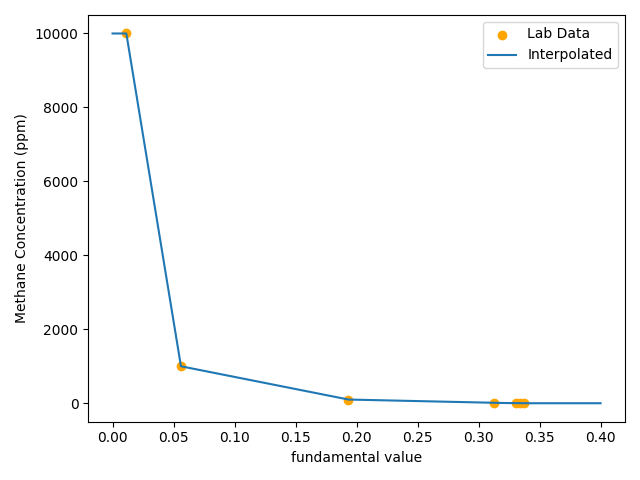
\includegraphics[width=0.6\textwidth]{figures/nopp_fundamental_calib_inverted.png}
    \caption{Fitted calibration curve for measurements of methane observed by Pythia.}
    \label{fig:nopp_curve}
\end{figure}

Compensation of Pythia's time response was also performed on post-calibrated data using the methodology described in \cite{miloshevich2004development} with a smoothing window of 5 minutes, and subsampling at a quarter of the time delay window. This methodology is sensitive to noise in the signal, which motivates the extreme sub-sampling that is performed. Fig.~\ref{fig:fund_corrected} shows the effect of smoothing, time-correction, and conversion on the direct signal recorded by Pythia before normalization. 

\begin{figure}[h!]
    \centering
    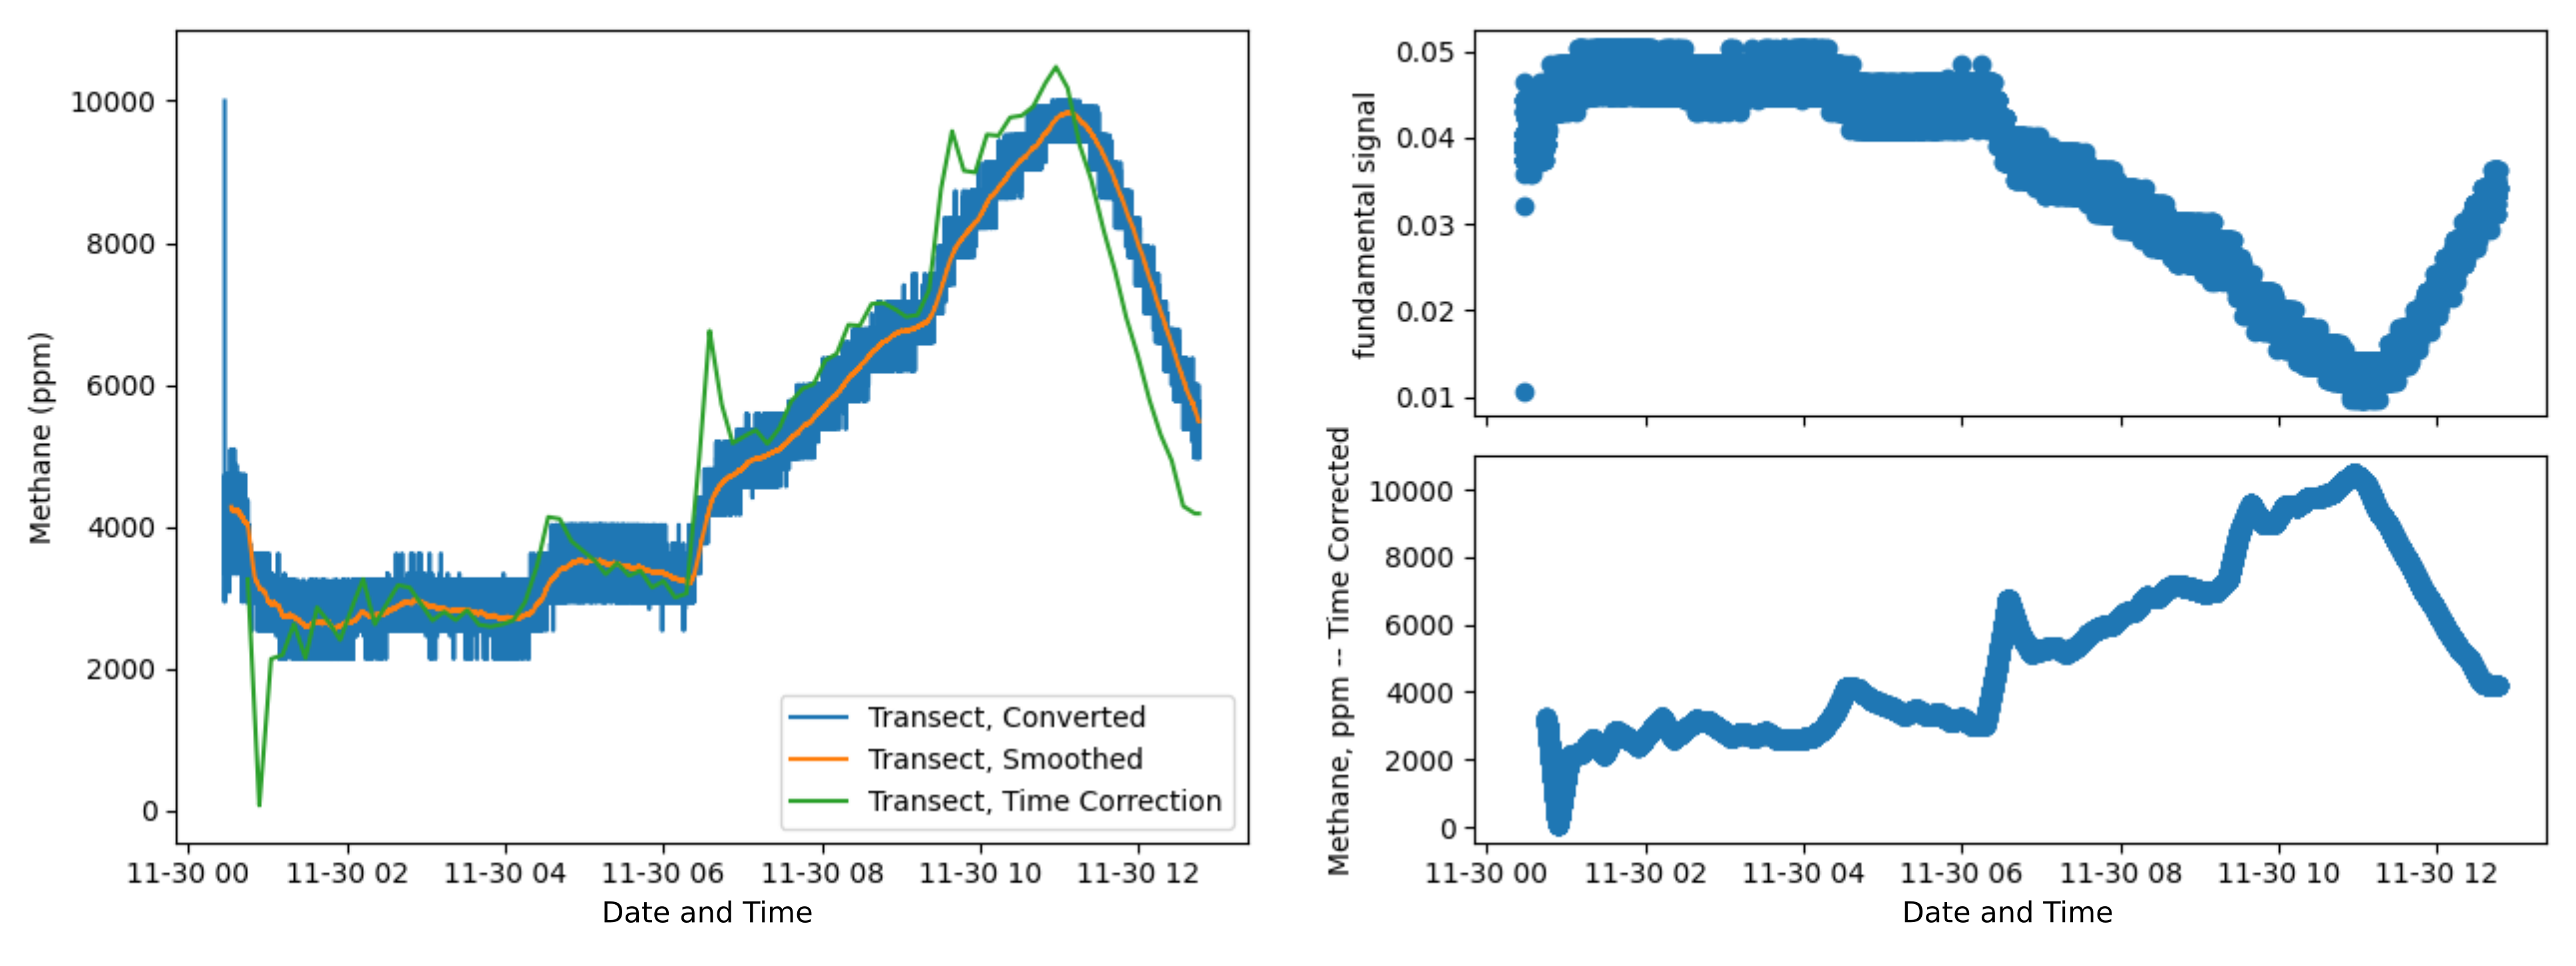
\includegraphics[width=1\textwidth]{figures/pythia_calibration.png}
    \caption[Pythia calibrated field data]{Calibration curve, smoothing, and time correction applied to Pythia observations during the transect, before reported normalization in the manuscript.}
    \label{fig:fund_corrected}
\end{figure}


\section{Depth-Correction}
\label{app:perception:depth}
Temperature, salinity, and oxygen are expected to be weakly stratified in the deep ocean. To remove these effects from data collected by AUV Sentry and the rosette, we fit a line to the average observations collected within binned 20 m intervals of observed depth for each platform separately. Separately computing the correction for each instrument additionally controls for small discrepancies in calibration between the platforms. Fig.~\ref{fig:linear_fits} compares these lines with the observations collected.

\begin{figure}[h!]
    \centering
    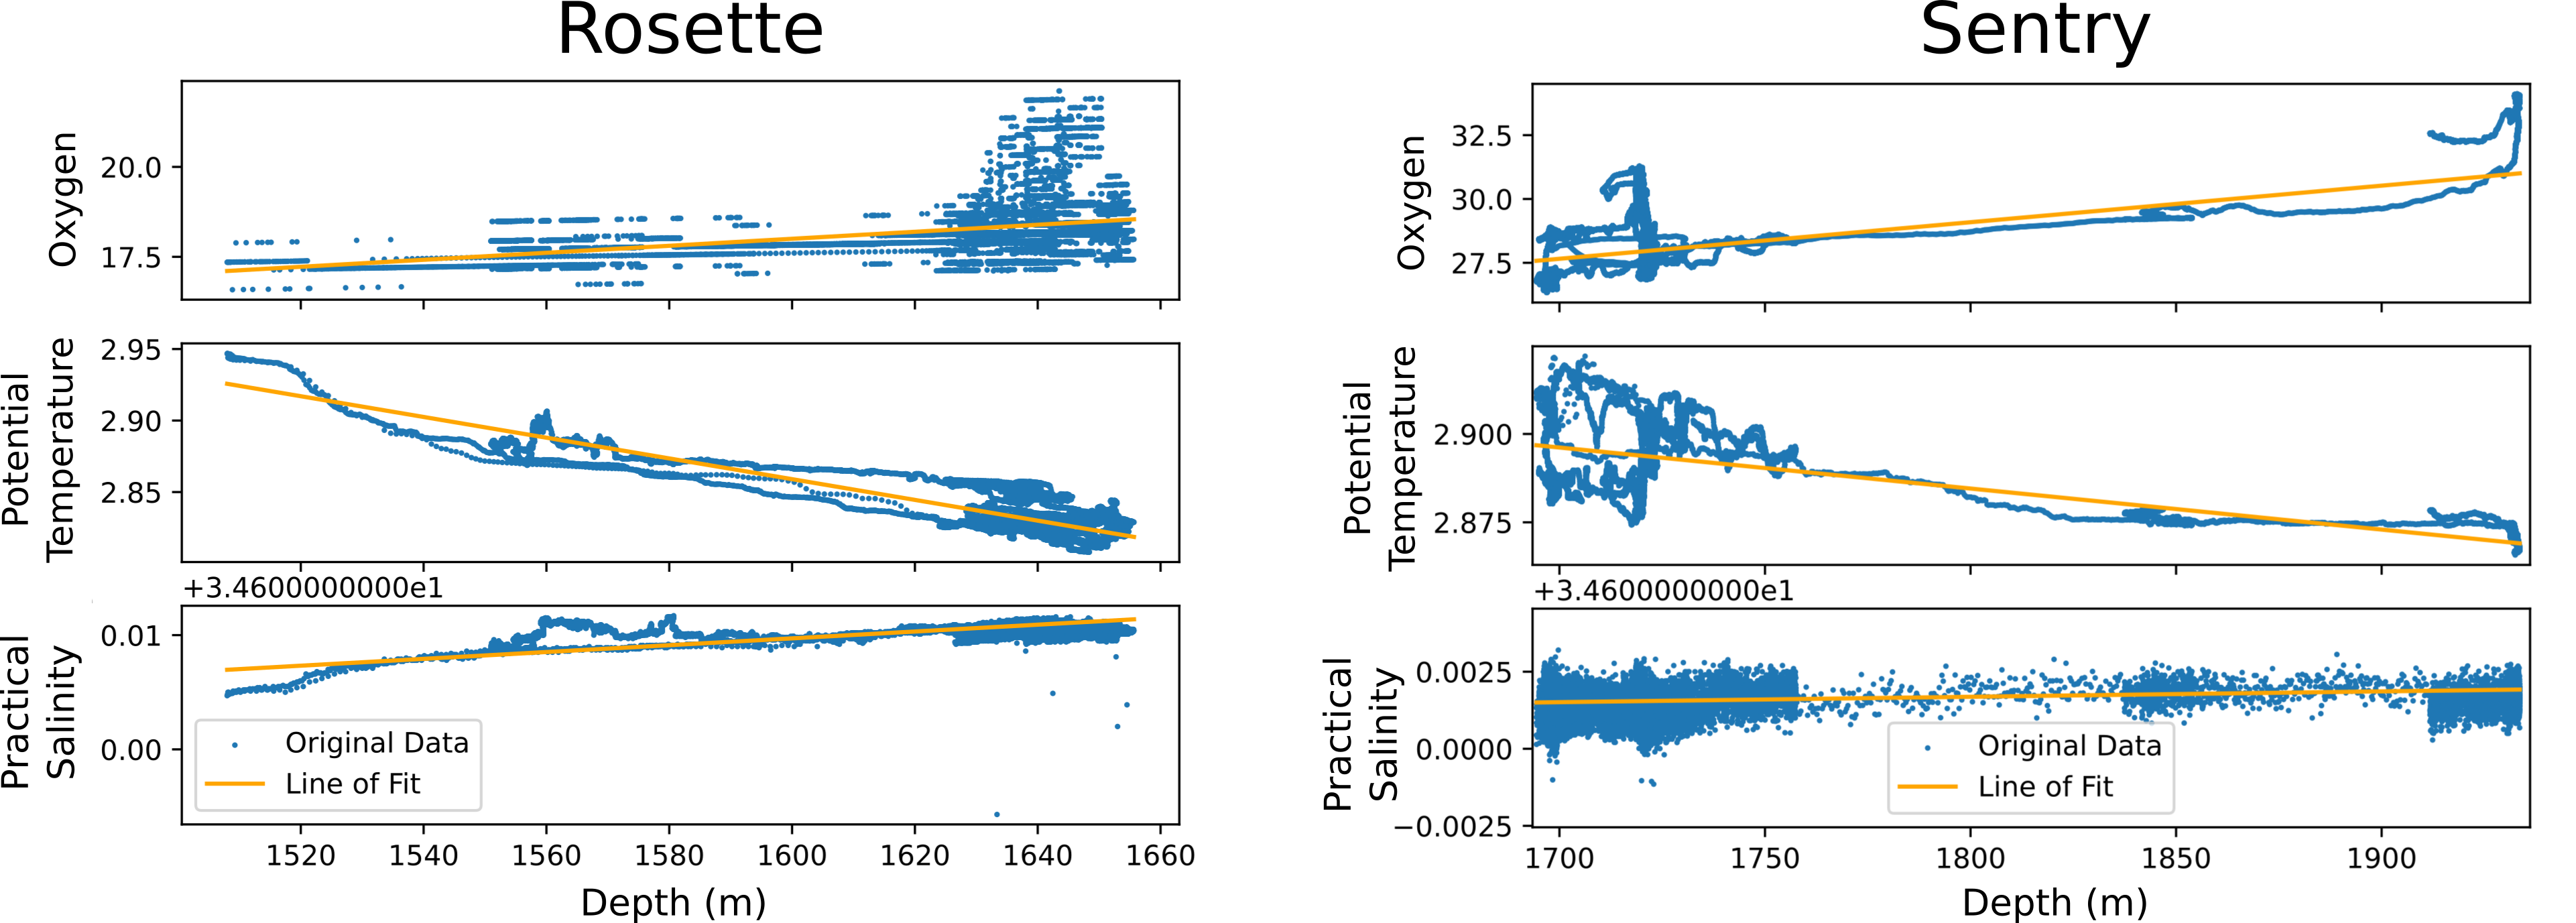
\includegraphics[width=1\columnwidth]{figures/depth_correction_plots.png}
    \caption[Functions used for depth normalization]{Linear functions are fit to data collected for oxygen, temperature, and salinity instruments on each platform separately. A residual value is then computed for each observation.}
    \label{fig:linear_fits}
\end{figure}

\section{Description of Plume Model for Transect Design}
\label{app:perception:model}
We adapted an idealized buoyant bent-plume model proposed by \cite{tohidi2016highly} for atmospheric bent plumes in a weakly stratified fluid in order to inform at what heights to deploy AUV Sentry and the rosette during the transect. We rewrite the system of equations provided in \cite{tohidi2016highly} as follows:

\begin{align}
    E &= \alpha\left|\frac{M}{Q} - u\cos(\theta)\right| + \beta\left|u\sin(\theta)\right| \\
    \frac{dQ}{ds} &= QE\sqrt{\frac{2(1 + \lambda^2)}{M\lambda}} \\
    \frac{dM}{ds} &= u\cos(\theta)\frac{dQ}{ds} + \frac{FQ}{M}\sin(\theta)\\
    \frac{d\theta}{ds} &= \left(\frac{FQ}{M}\cos(\theta) - u\sin(\theta)\frac{dQ}{ds}\right)\frac{1}{M}
\end{align}
\begin{align}
    \frac{dF}{ds} &= -QN^2\sin(\theta)\\
    \frac{dX}{ds} &= \cos(\theta)\\
    \frac{dZ}{ds} &= \sin(\theta)
\end{align}

\noindent where $E$ is a mixing entrainment coefficient which considers both vertical and horizontal mixing and is weighted by parameters $\alpha$ and $\beta$, $u$ is the crossflow velocity which can be a function of depth and time, $\lambda$ is a parameter which modifies the ellipse which describes the plume envelope, $Q$ is specific volume flux, $M$ is specific momentum flux, $F$ is specific buoyancy flux, $\theta$ is plume centerline trajectory angle, $s$ is the plume centerline trajectory, $X$ is distance along a coordinate axis aligned with the plume centerline, $Z$ is height with respect to plume source along a vertical axis, and $N^2$ is the Brunt-V\"ais\"al\"a frequency, computed with respect to the density gradient at the reference depths of the source and plume height.

The system of equations essentially yields a ``snapshot'' of a plume envelope at some moment in time. For time-varying crossflows, multiple snapshots can be computed for different moments in time (different crossflow orientations and magnitudes) and chained together in a common coordinate reference system in order to track a plume trajectory. For the purposes of determining which heights to deploy AUV Sentry and the rosette for the transect, we compute a prototypical envelope and use the estimated bent nonbuoyant plume height to set the transect depths/altitudes.

The initial conditions for solving this system of ordinary differential equations are set via estimates of vent characteristics including exit velocity, temperature, salinity, and area. Specifically:

\begin{align}
    Q_o &= \lambda V_v \frac{A_v}{\pi} \\
    M_o &= Q_o V_v \\
    F_o &= -g10^{-4}(T_v - T_z)Q_o \\
    \theta_o &= \frac{\pi}{2}
\end{align}

\noindent where $V_v$ is exit velocity at the vent orifice, $A_v$ is the vent orifice area, $T_v$ is the temperature at the orifice area, and $T_z$ is the expected temperature of ambient seawater at the estimated vent depth. Note that initial buoyancy flux is primarily driven by temperature changes, as we anticipate this to be the major driver of density gradients at our measurement scale. Expected salinity gradients could be similarly considered.

Estimated vent characteristics and crossflow were selected based on empirical observations of the deep sea vents located along the northern Guaymas Basin ridge and observations of current magnitude collected by a current tiltmeter deployed by ROV Jason during several days of the research cruise. Table~\ref{tab:params} lists the settings for planning the transect selected for these characteristics. Background salinity and temperature profiles were computed according to standard Pacific Ocean temperature and salinity functions as described in \cite{speer1989model}; additionally the equation of state for computing density profile from salinity and temperature measurements was used also as defined in \cite{speer1989model}. The prototypical plume is computed with a source located at 1850 m depth.

\begin{table}[h!]
    \centering
    \begin{tabular}{c|c|l}
        Parameter & Assignment & Description \\
        \hline
        $\lambda$ & 1.0 & Ratio of elliptical axes of the plume envelope \\
        $V_v$ & \SI{0.58}{\meter\per\second} & Exit velocity of fluids at vent orifice \\
        $A_v$ & \SI{0.82}{\meter\squared} & Area of vent orifice \\
        $T_v$ & \SI{340}{\celsius} & Temperature of fluids at vent orifice \\
        $\alpha$ & 0.15 & Longitudinal shear-driven mixing coefficient \\
        $\beta$ & 0.19 & Transverse shear-driven mixing coefficient \\
        $u$ & \SI{0.1}{\meter\per\second} & Magnitude of crossflow \\
    \end{tabular}
    \caption{Parameter, vent characteristics, and ambient crossflow setting used for transect design.}
    \label{tab:params}
\end{table}

The prototypical plume envelope computed in this manner estimates a nonbuoyant plume depth between 1570-1750 m (Fig.~\ref{fig:plume_envelopes}). AUV Sentry is altitude limited in order to keep a fix on the ocean floor for navigation; it is set to its maximum altitude of \SI{120}{\meter} in order to intersect with the bottom of the estimated nonbuoyant layer; this corresponds to a depth of approximately 1700 m throughout the basin. The rosette can be arbitrarily fixed to a height, but so as not to interfere with AUV Sentry operations and to sample a different point in the estimated nonbuoyant layer, a depth of 1650-1600 m was targeted.

\begin{figure}[h!]
    \centering
    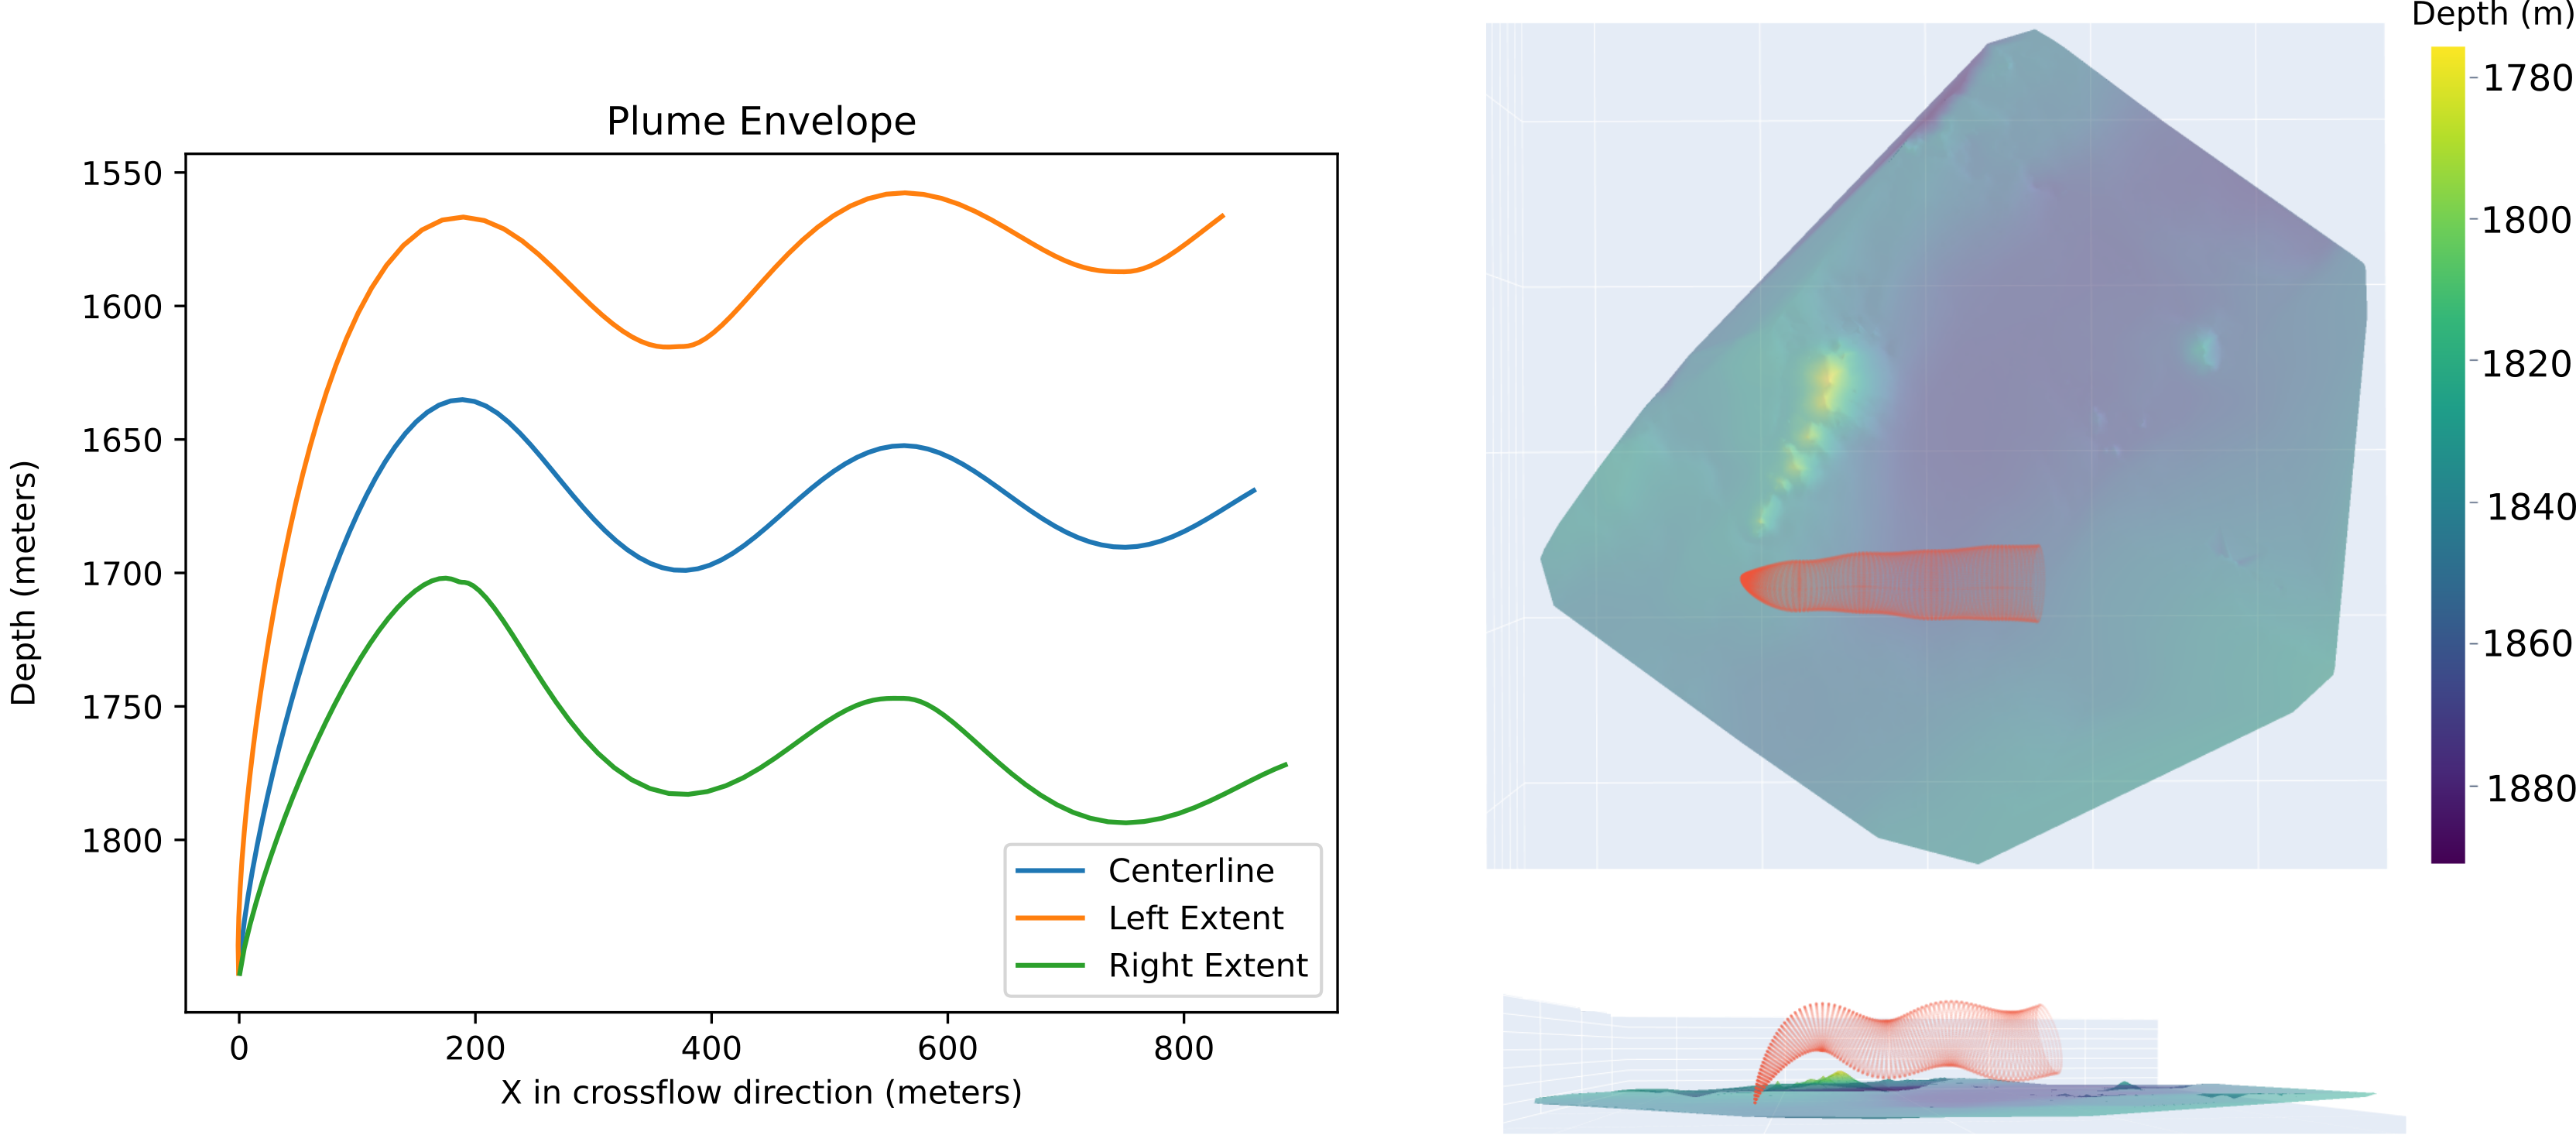
\includegraphics[width=1\columnwidth]{figures/plume_envelopes.png}
    \caption[Plume model for transect design]{A prototypical plume estimate according to the modified buoyant plume model in crossflow. The same envelope is plotted with respect to absolute depth (with a source located at 1850 m) on the left, and illustratively in the context of the hydrothermal ridge on the right.}
    \label{fig:plume_envelopes}
\end{figure}

%%%%%%
% Appendix B
%%%%%%
\chapter{\PHORTEX Algorithm Performance}
\label{app:phortex}

\section{Convergence Characteristics of Trajectory Optimizer}
The trajectory optimization scheme presented in \cref{sec:to} uses a gradient-based optimizer with trust-bounded constraints in order to set the parameters of a set of lawnmower trajectories. In general, this is a difficult optimization problem, as analytical gradients that map the defining parameters of a lawnmower trajectory (orientation, size, and location) are not available, and must be numerically approximated. Moreover, by defining trust constraints, jumping between minima could be made more difficult, as the approximated gradients may lead through unsafe (un-trusted) space. In practice, this meant that initializing each lawnmower in a chain to be near a ``good trajectory'' was important. In the case of charting hydrothermal plumes, a ``good'' trajectory would be one approximately aligned with the estimated crossflow. As \PHUMES provides complete access to this information, it is generally easy to seed the trajectories to be near a performant minima. This leads to relatively fast convergence of the optimizer for each element in the chain. In \cref{fig:phortex_chain} there is an example a snapshot along the path to convergence for each link in a chain visualized, and the convergence plot. As is evidenced in the plot, a long travel time between chains is accumulated; this is likely because ``flipping'' a trajectory to shorten this distance would be a prohibitively difficult step in the nonlinear, constrained space that the optimizer operates.

\begin{figure}[h!]
    \centering
    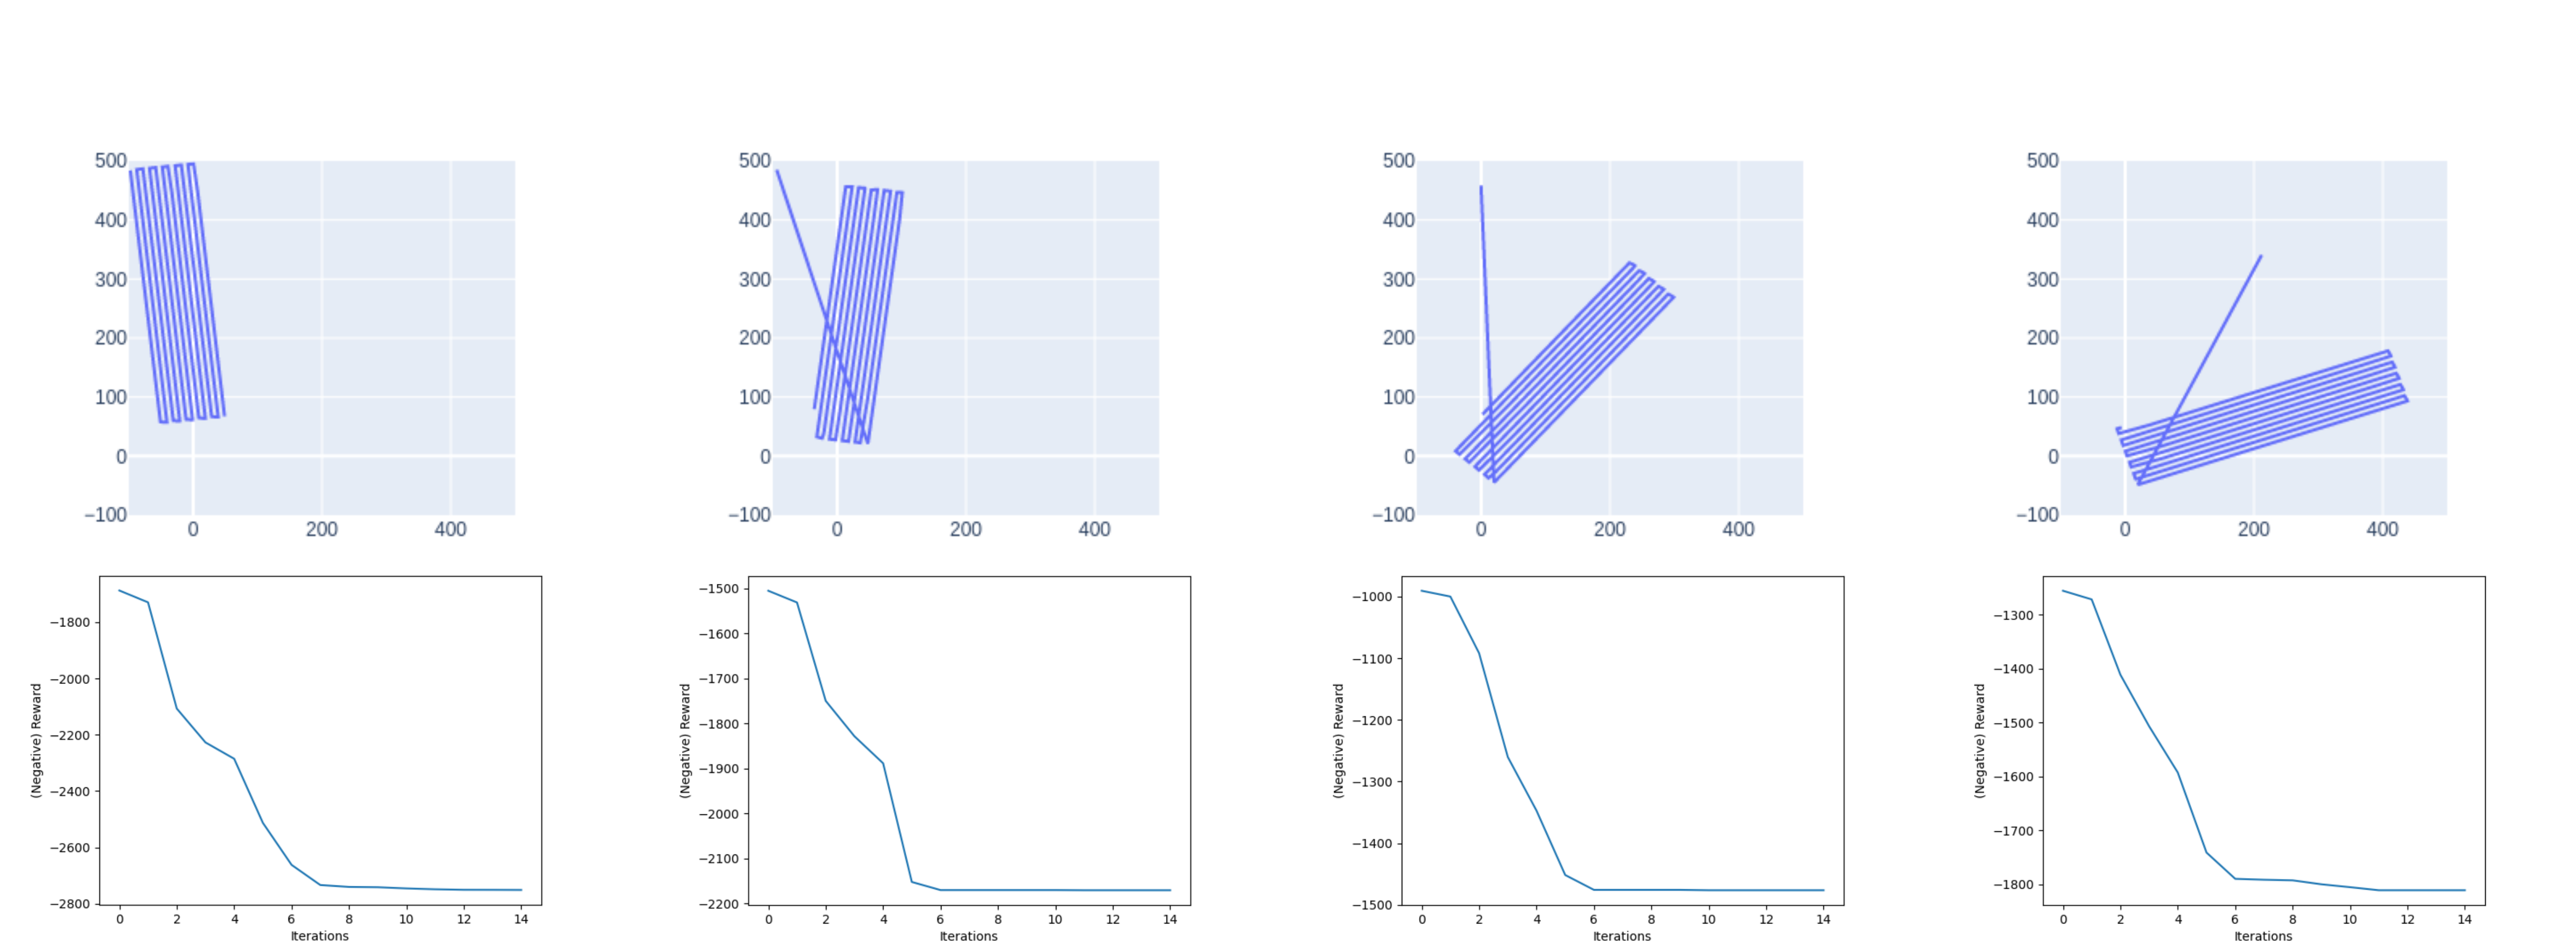
\includegraphics[width=1\columnwidth]{figures/phortex_iterations.png}
    \caption[\PHORTEX optimization performance]{Example snapshots of each link in a \PHORTEX trajectory from a \cref{chap:phortex} simulation trial, and their corresponding convergence plots. While trajectories show good agreement with the current function and size of a plume expression as modeled by \PHUMES, a long travel time between chains is accumulated; this is likely because ``flipping'' a trajectory to shorten this distance would be a prohibitively difficult step in the nonlinear, constrained space that the optimizer operates.}
    \label{fig:phortex_chain}
\end{figure}

\section{Chaining Characteristics of \PHUMES}
For computational reasons, it is typically not possible to run the chains for thousands of samples while in the field, and the chains must be arbitrarily cut short in order to generate a plan. For this reason, it is interesting to look at the chaining properties. For a simulation trial, as described in \cref{chap:phortex}, we show the chains and probability densities for each of vent area, vent fluid velocity, and entrainment coefficients in \cref{fig:phumes_sim_chain}. As evidenced by the multimodal area plot, we observe that the relationship between the parameters is complicated; in general, an inverse problem like the one we have posed for \PHUMES is a challenge to infer. What is promising however is that probability densities are being concentrated in areas that make sense (as observed by a mode at 0.8 for area), and that the \emph{combinations} of learned parameters are sensible --- a large area should be coupled with a slow or medium velocity; a high velocity should be paired with a small area --- based on the relationships between parameters and how they manifest in the ultimate shape of the plumes in the 3D Cartesian space.

\begin{figure}[h!]
    \centering
    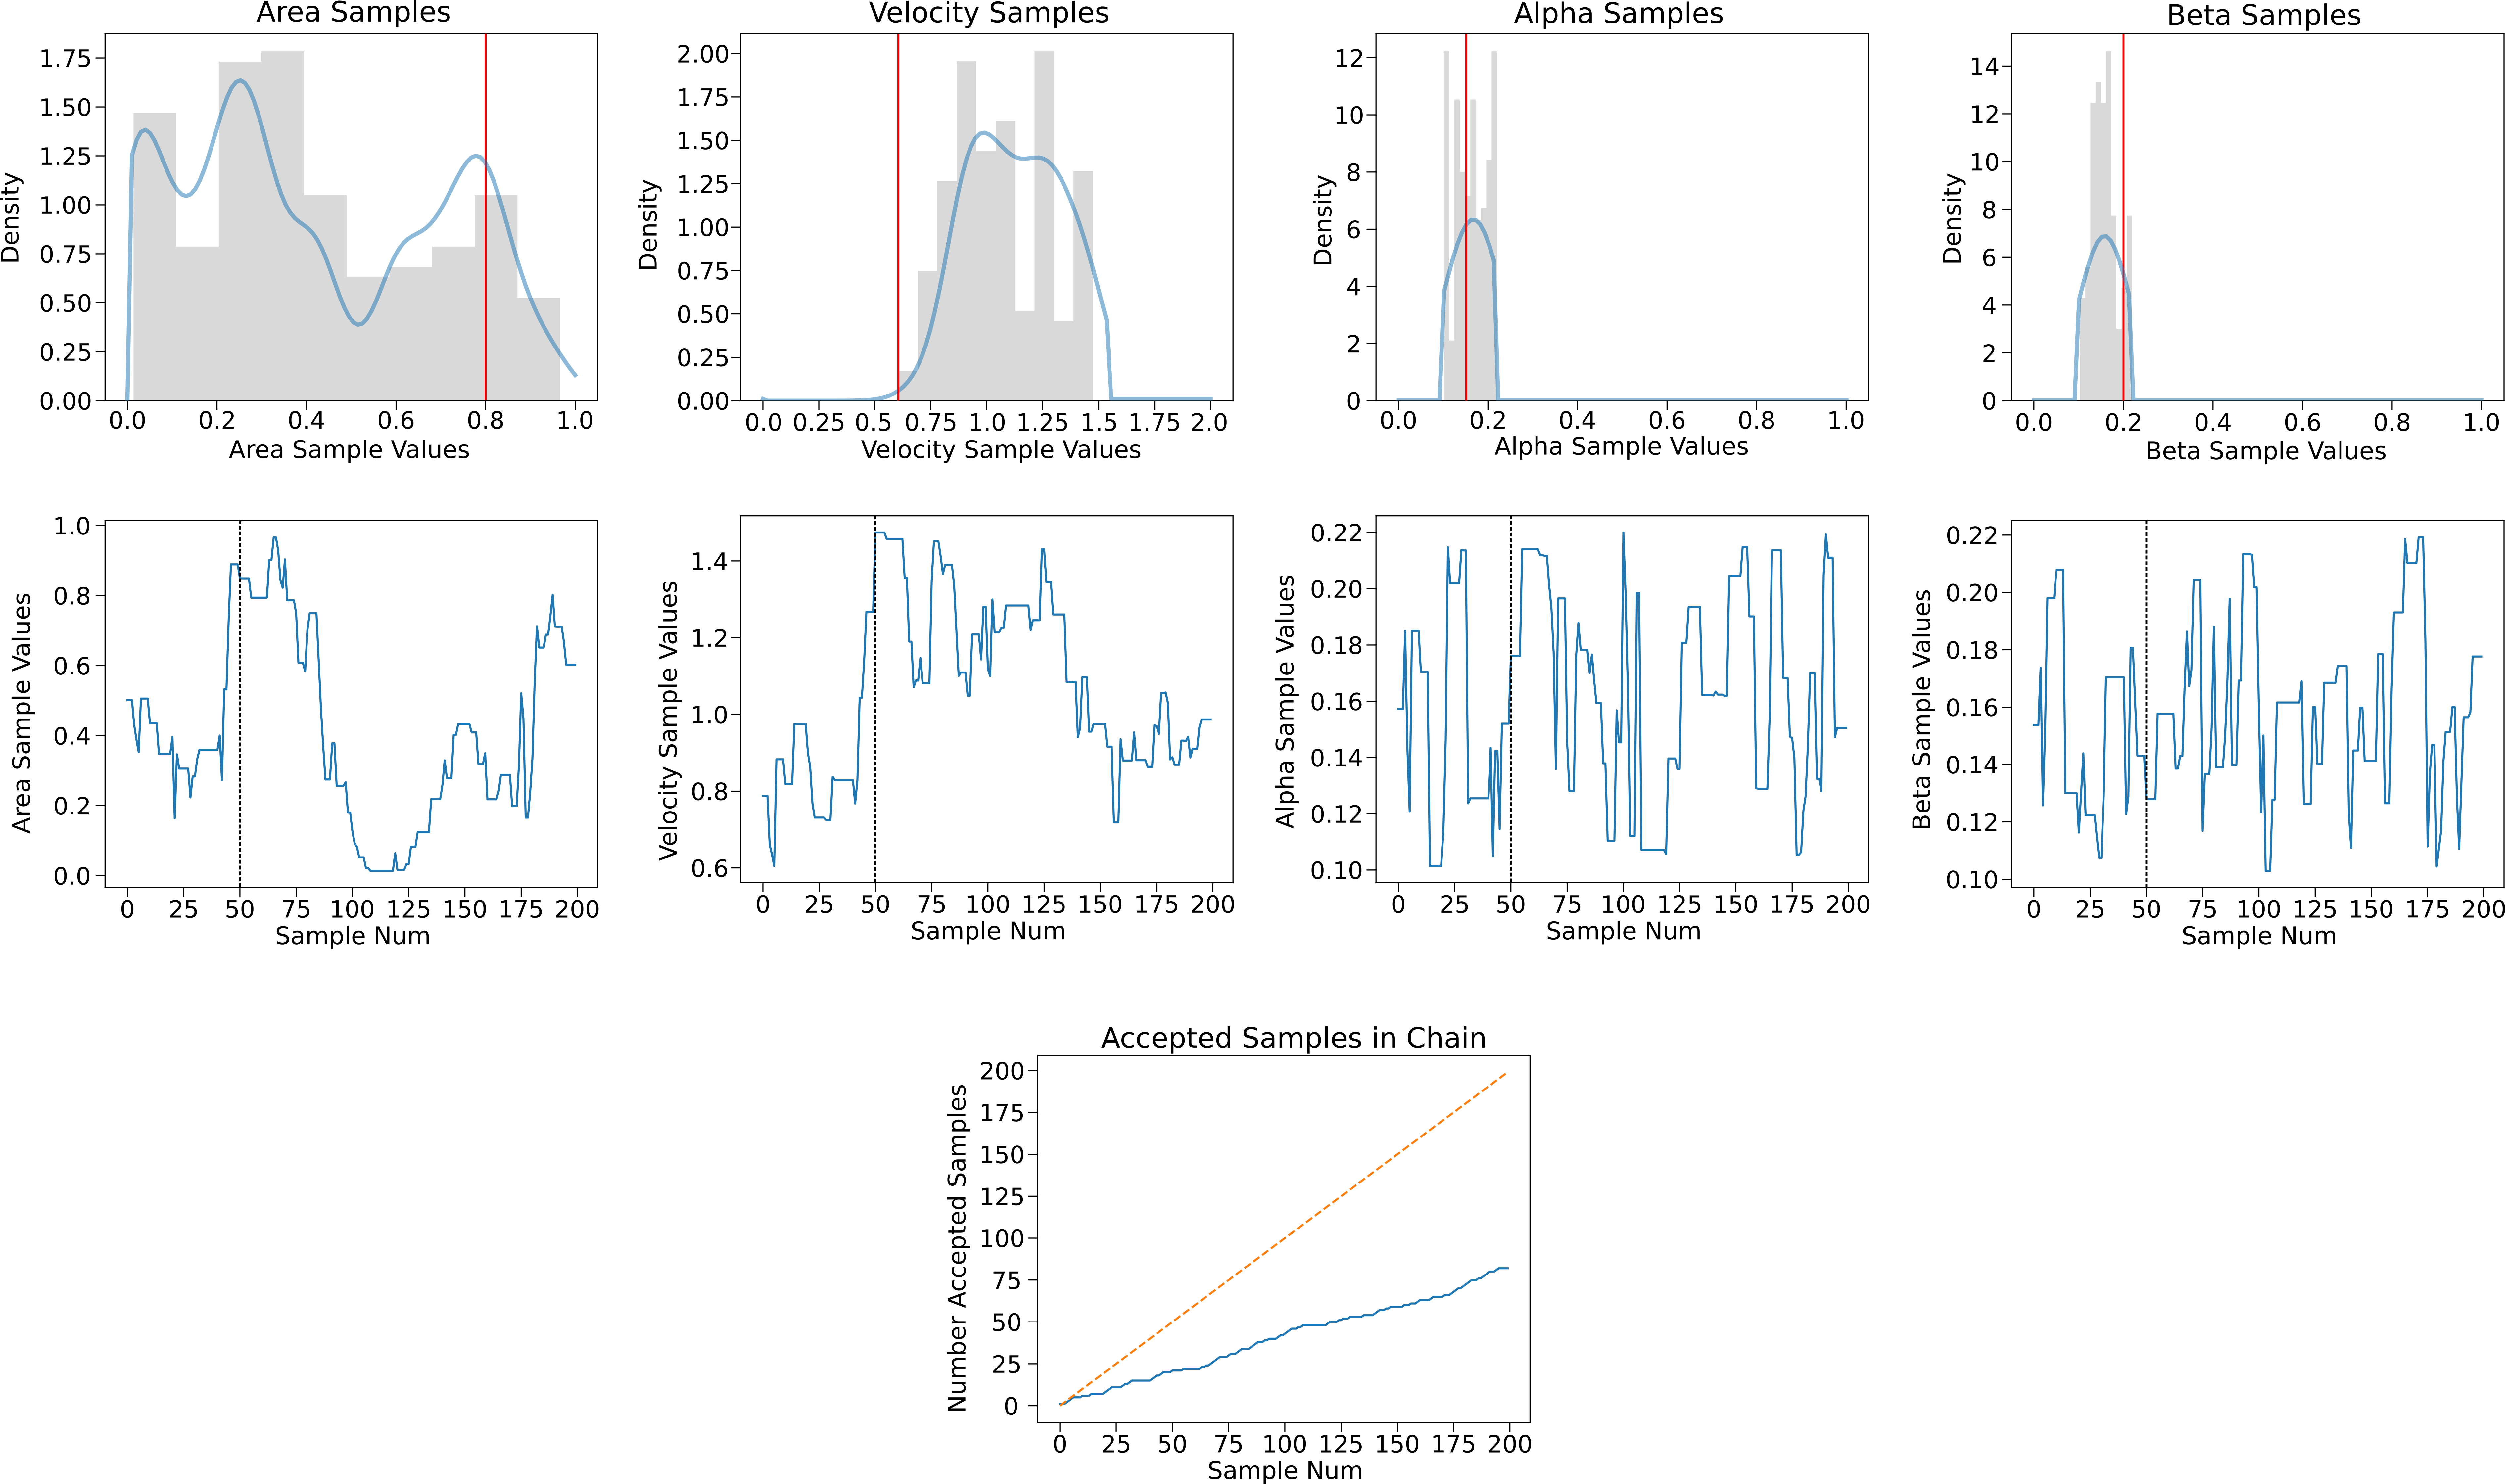
\includegraphics[width=1\columnwidth]{figures/phumes_trial_chain.png}
    \caption[\PHUMES simulation chain]{An example chain from a simulation trial as described in \cref{chap:phortex}. The last 150 samples in each chain is used to compute the distributions in blue; all samples are shown in gray in the top plots. Red lines in the top plots indicate the generating environment value for the simulation. The chain efficiency is approximately 37.5\%.}
    \label{fig:phumes_sim_chain}
\end{figure}

We can also look at how convergence may change for longer chains. In an exemplar trial (\cref{fig:phumes_long_chain}), a chain is run for 650 samples, and the last 500 samples are used to compute densities. The acceptance rate stays approximately the same, at about 34\%. However, the distributions have generally improved with respect to placing more density at the parameters that defined the true underlying environment. As evidenced in the area and velocity sampling plots, there is still some exploration of the state space being performed by the chains; this suggests that true convergence of these chains may either take a long time, or the information content of the data that is available to explore the state space leads to ambiguous ``wells'' which the chains would ``bounce'' between for long durations. This suggests that other Monte Carlo techniques, such as Hamiltonian Monte Carlo~\autocite{duane1987hybrid}, may be of interest in adaptation of this work, to accelerate chain exploration.

\begin{figure}[h!]
    \centering
    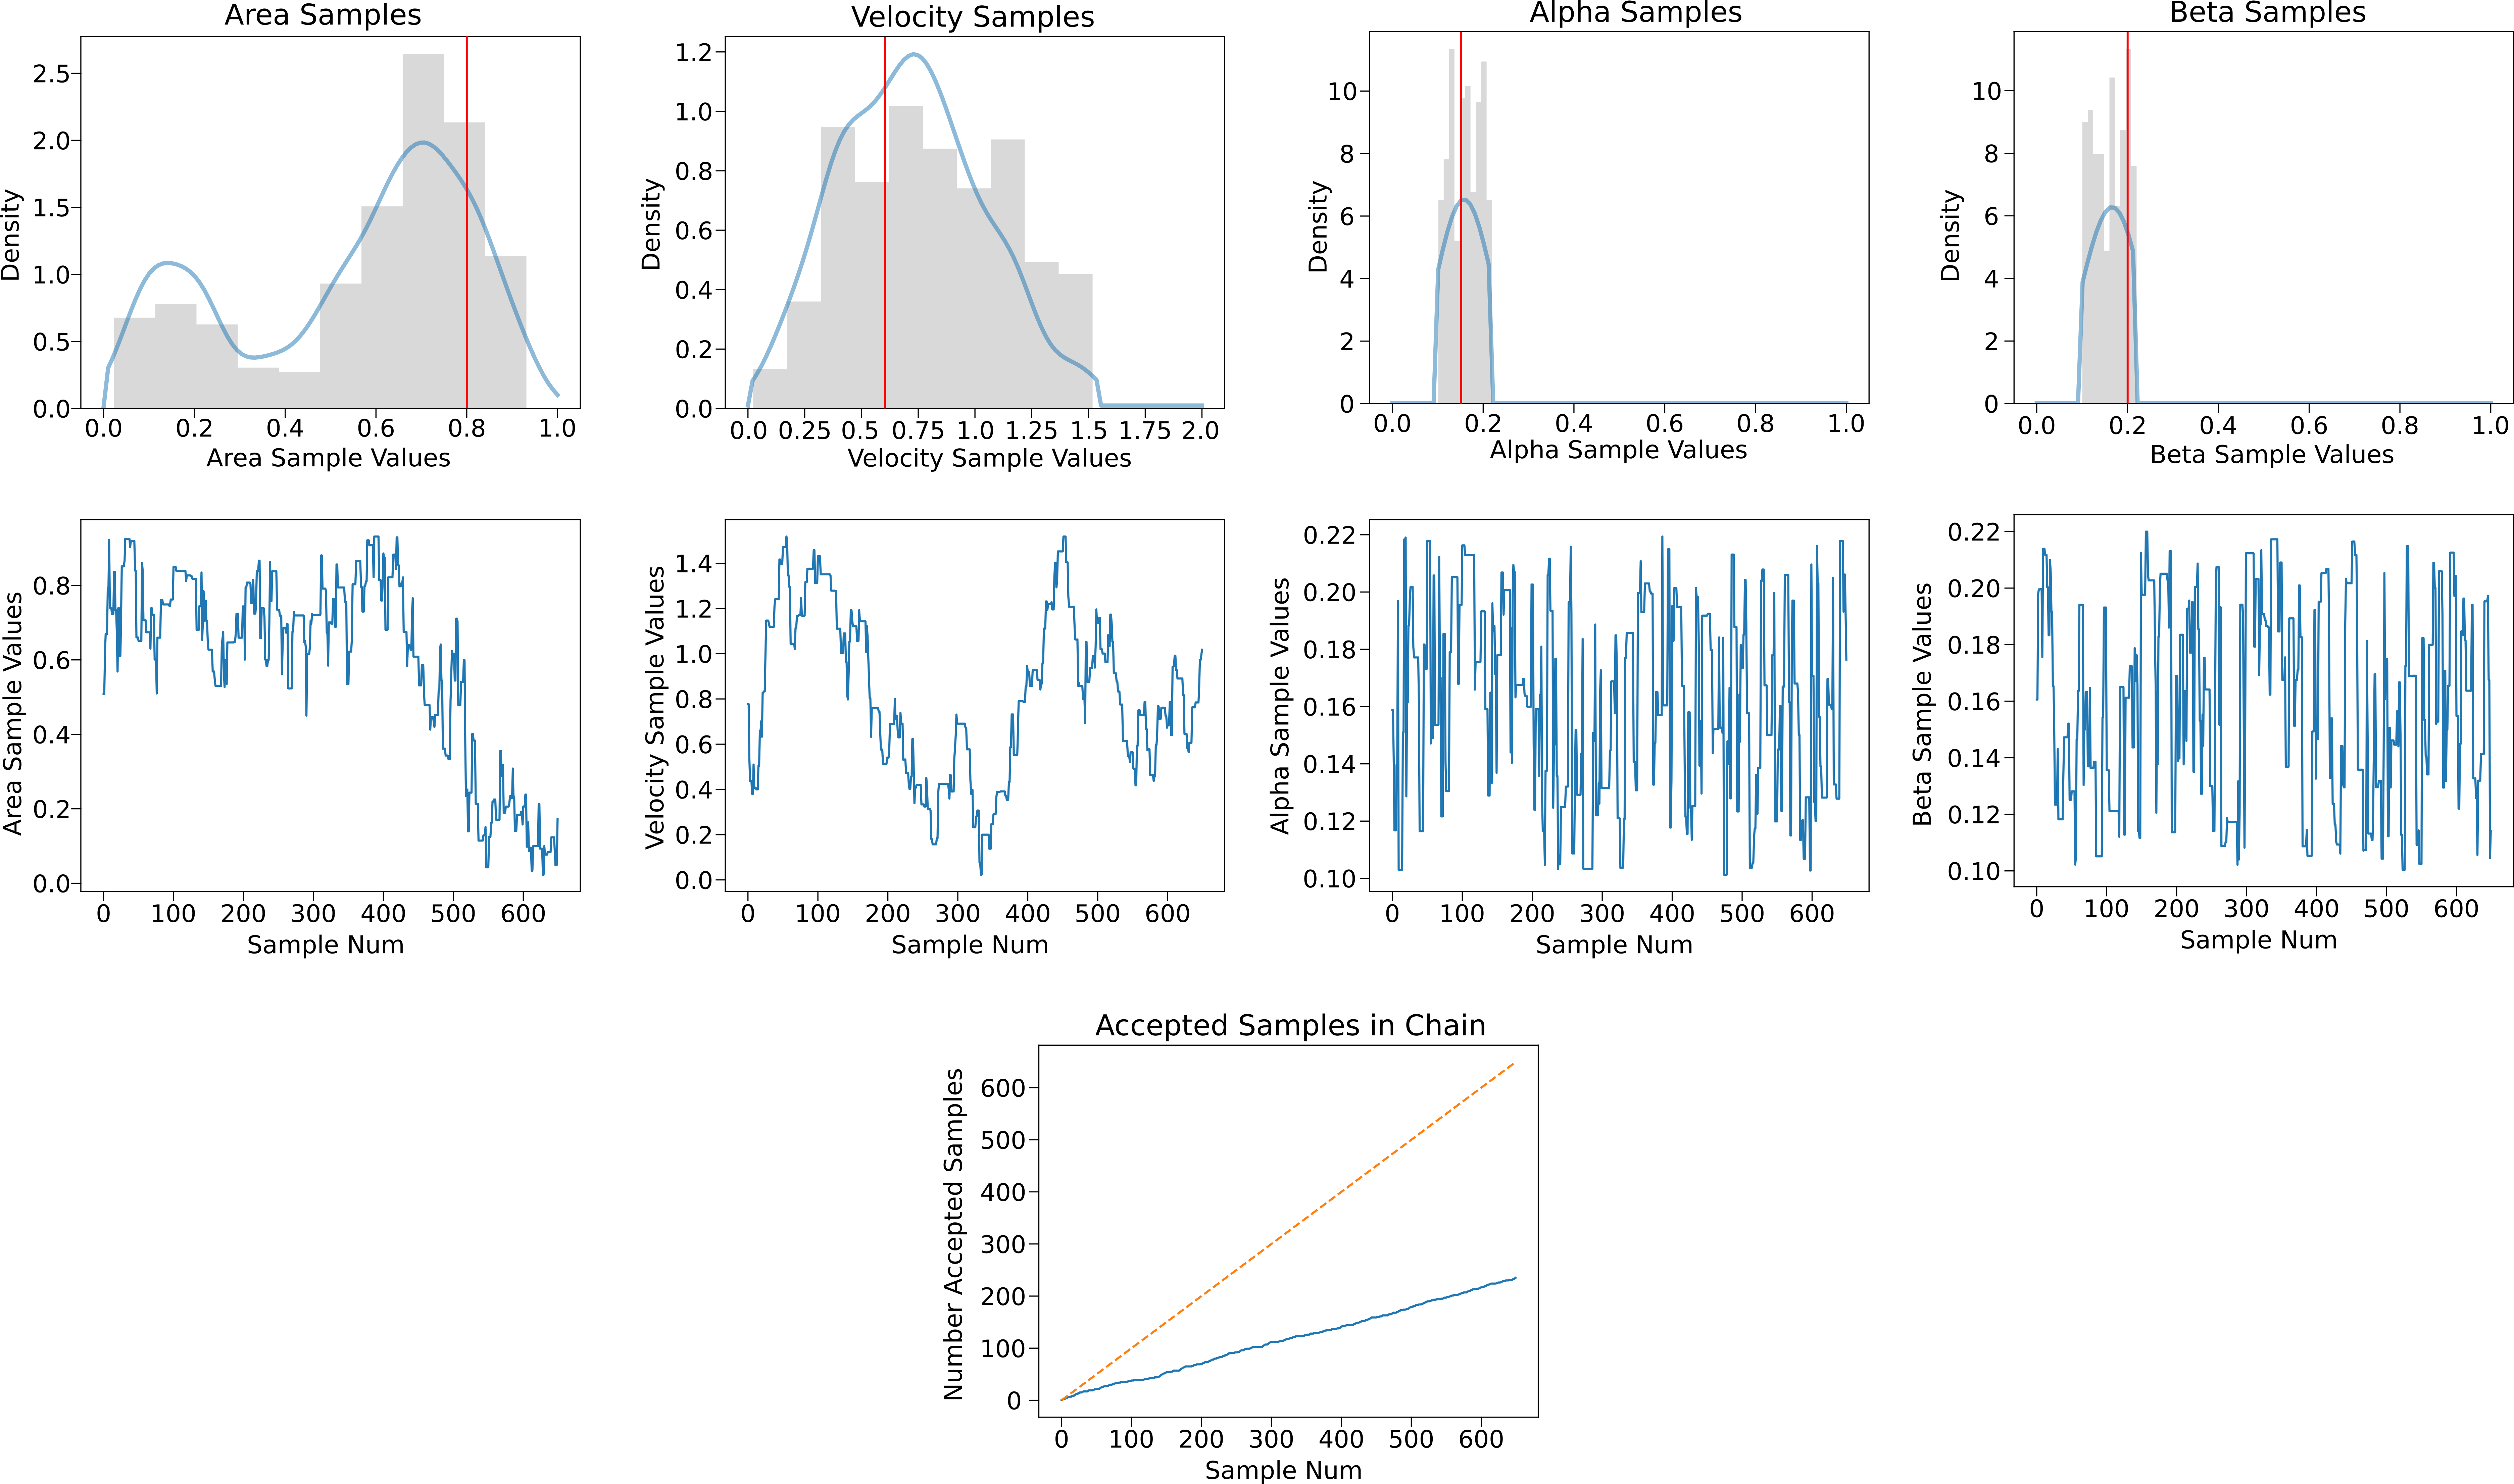
\includegraphics[width=1\columnwidth]{figures/phumes_long_chain.png}
    \caption[\PHUMES long chain]{An example chain from a simulation trial as described in \cref{chap:phortex}, but run for 650 samples; the last 500 are used to compute the distributions in blue with all samples shown in gray in the top plots. Red lines in the top plots indicate the generating environment value for the simulation. The chain efficiency is approximately 34\%.}
    \label{fig:phumes_long_chain}
\end{figure}

\section{Code Availability}
\td{Might be nice to link to the code here and have some brief documentation on how to use it.}


% This ensures that the subsequent sections are being included as root
% items in the bookmark structure of your PDF reader.
\bookmarksetup{startatroot}
\backmatter

  \begingroup
    \let\clearpage\relax
    \glsaddall
    \printglossary[type=\acronymtype]
    \newpage
    \printglossary
  \endgroup

  \printindex
  \printbibliography

\end{document}
